%*******************************************************
% Chapter 2 — DRAFT v2 (avril 2026)
%*******************************************************
\chapter{Structures économiques de l'information}\label{ch:economics}

\begin{center}
\textit{Résumés des dimensions --- document de travail écrit par Rémi $\to$ Franck, 27 mai 2026}
\end{center}

\bigskip

Ce qui suit résume chacune des dix dimensions du chapitre. Pour chaque dimension~: une définition, ce qu'elle étudie, d'où elle vient dans le chapitre~1, les références mobilisées, et ce qui en sort. Chaque dimension produit des hypothèses  (certaines sont des faits "plutôt" établis, d'autres des mécanismes "plausibles", d'autres encore des conjectures; la classification n'est pas encore stabilisée et les niveaux se mélangent un peu pour le moment, mais j'ai en tête une hiérarchie (établi / fait stylisé / hypothèse / conjecture) qu'il faudra rendre explicite. L'analyse procède ici dimension par dimension~; mais je pense qu'une deuxième étape --- "l'intégration macroéconomique" --- devrait traiter les croisements entre dimensions (pas encore fait). L'ensemble pourrait donc former une boîte à outils dans laquelle on piochera pour la modélisation~...

% -----------------------------------------------------------------------------
\paragraph{Dimension~1 --- Propriétés du bien informationnel.}
Le bien informationnel est tout bien dont la valeur économique dérive de son contenu en information, qu'il soit incorporé dans un support physique (câble, processeur, data center) ou codé (algorithme, données, modèle entraîné). La dimension examine quelles propriétés de ce bien déterminent ses effets économiques.

\subparagraph{Objet.}
Le même objet technique --- un service d'IA, un câble sous-marin, une tabulatrice --- contient des composantes aux propriétés économiques opposées. Les poids d'un modèle de langage sont copiables sans perte (ce que la théorie appelle «~non-rivalité~»~...). Le GPU qui fait tourner l'inférence et l'énergie qu'il consomme ne sont disponibles que pour un seul utilisateur à la fois (ce qu'on appelle «~rivalité~»). La section examine quelles propriétés du bien informationnel --- rivalité, excluabilité, codifiabilité, complémentarité, régime de dépréciation --- déterminent ses effets économiques, en les appliquant non pas au bien dans son ensemble mais à chacune de ses couches (substrat physique d'un côté, contenu codifié de l'autre).

\subparagraph{Ce qui a induit la dimension dans le chapitre~1.}
Trois régularités historiques. (i)~Chaque réseau de communication étudié --- télégraphe, téléphone, mécanographie --- converge vers une forme de monopole, mais par des combinaisons différentes des moyens de restreindre l'accès~: Western Union contrôle les fils, IBM couple location et cartes propriétaires, AT\&T combine les trois. Le résultat est le même, le chemin varie. (ii)~Le domaine des savoirs transmissibles s'étend d'une vague à l'autre~: le télégraphe transmet les cotations du coton, la mécanographie codifie les procédures administratives, l'IA générative produit quelque chose qui ressemble à du diagnostic --- mais par un canal différent de la codification classique. (iii)~Les systèmes informationnels intégrés contiennent toujours des couches à temporalités incompatibles~: le réseau télégraphique dure quarante ans mais porte des messages éphémères~; le data center dure vingt-cinq ans mais héberge des modèles qui se déprécient en douze mois.

\subparagraph{Références mobilisées.}
Samuelson 1954, Arrow 1962, Lancaster 1966, Polanyi 1966, Rosen 1974, Hill 1977, Milgrom et Roberts 1990, Ostrom 1990, Shapiro et Varian 1999, Lessig 1999, Cowan et Foray 2000, Quah 2003, Benkler 2006, Hess et Ostrom 2007, Boldrin et Levine 2008, Zittrain 2008, Jones et Tonetti 2020, Haskel et Westlake 2018, Johansen 1959, Arthur 1989, Dixit et Pindyck 1994, Kaplan et al.\ 2020, Cottier et al.\ 2025. Ancrage historique~: Steinwender 2018, Juhász et al.\ 2018, Beauchamp 2010, Mounier-Kuhn 2010, Heide 2009.

\subparagraph{Ce qui en sort --- trois hypoth\`eses.}

\emph{Premi\`ere hypoth\`ese.} Un bien informationnel contient des composantes dont les unes sont copiables \`a co\^ut nul et les autres sont physiquement rares. Ces deux types de composantes ne suivent pas les m\^emes trajectoires \'economiques~: la composante copiable tend vers le prix z\'ero (parce que le co\^ut de reproduction est nul), tandis que la composante rare reste soumise \`a la raret\'e physique et \`a la tarification standard. Le mod\`ele d'affaires doit r\'esoudre cette tension interne, et la r\'esolution varie selon les \'epoques et les configurations --- parfois la rente va \`a la couche rare, parfois \`a la couche copiable, parfois aux deux. Un mod\`ele \'economique qui agr\`ege les deux composantes dans un seul facteur ne voit pas cette divergence (par exemple~: Western Union tire sa valeur des fils, pas des cotations transmises~; les poids de Llama sont distribu\'es gratuitement pendant que le march\'e des GPU d'inf\'erence est en p\'enurie). \textbf{H-D1.1~: les couches rivales et non-rivales d'un m\^eme bien informationnel suivent des trajectoires \'economiques distinctes, et un mod\`ele qui les agr\`ege dans un seul facteur ne peut pas voir cette divergence} (\emph{tension de commodification partielle}~? ou \emph{dualit\'e rival/non-rival intra-bien}~?).

\emph{Deuxi\`eme hypoth\`ese.} Le domaine des savoirs qui deviennent des biens transmissibles s'\'etend dans le temps, mais par au moins deux op\'erations distinctes. La premi\`ere consiste \`a transformer un savoir en r\`egles explicites, intelligibles, v\'erifiables --- un protocole, un standard, un syst\`eme de gestion. La seconde consiste \`a ing\'erer un corpus massif et \`a produire une fonction qui imite le r\'esultat d'un savoir-faire sans le rendre intelligible --- un mod\`ele de langage, un mod\`ele pr\'edictif. Les deux op\'erations partagent certaines propri\'et\'es \'economiques (transmissibilit\'e, reproductibilit\'e \`a co\^ut marginal faible), mais leurs profils de co\^ut diff\`erent radicalement~: la premi\`ere co\^ute du travail intellectuel de formalisation, la seconde co\^ute du compute d'entra\^{\i}nement qui se traduit directement en \'energie. \textbf{H-D1.2~: le mix codification / "compression statistique" dans un syst\`eme num\'erique d\'etermine son profil \'energ\'etique et constitue une variable de sc\'enario} (la premi\`ere op\'eration correspond \`a ce que Cowan et Foray appellent \emph{codification}~; pour la seconde, je propose le terme \emph{"compression statistique"}~? --- il n'est pas \'etabli dans la litt\'erature).

\emph{Troisi\`eme hypoth\`ese.} Dans les syst\`emes informationnels int\'egr\'es, des couches \`a temporalit\'es de d\'epr\'eciation incompatibles coexistent dans le m\^eme objet technique et ne fonctionnent pas les unes sans les autres. Quand ces couches sont physiquement li\'ees, le verrouillage qui en r\'esulte est asym\'etrique~: les couches lentes contraignent les choix dans les couches rapides, mais le renouvellement des couches rapides n'\'elimine pas l'inertie des lentes. Ce ph\'enom\`ene est r\'ecurrent sur deux si\`ecles~; ce qui change dans le r\'egime contemporain, c'est son amplitude --- le rapport entre la couche la plus lente et la plus rapide atteint 1:20 dans les data centers (b\^atiment 25~ans, PPA 10--15~ans, GPU 3--5~ans, mod\`ele 12--18~mois), contre $\sim$1:5 dans les cas historiques. \textbf{H-D1.3~: le capital qui produit le bien informationnel lie physiquement des couches \`a temporalit\'es incompatibles, et le verrouillage qui en r\'esulte est asym\'etrique --- les couches lentes contraignent les rapides} (extension du mod\`ele putty-clay de Johansen 1959 \`a plusieurs couches (si j'ai bien compris...)~; la liaison entre composants est ce que Milgrom et Roberts appellent \emph{supermodularit\'e}~?~; la perte de valeur de la couche rapide est ce que Marx appelle \emph{d\'epr\'eciation morale}~?).

\subparagraph{Questions et incertitudes.}
\begin{itemize}
\item Le terme \og~compression statistique~\fg{} est une proposition --- est-ce le bon mot~? Faut-il un autre terme~?
\item Pourquoi exactement deux canaux d'extension (codification et compression) et pas trois ou cinq~? La justification est dans ma t\^ete mais pas assez dans le texte.
\item Le passage de 1:5 \`a 1:20 dans les temporalit\'es des couches change-t-il \emph{qualitativement} quelque chose, ou est-ce juste plus du m\^eme~?
\end{itemize}


% -----------------------------------------------------------------------------
\paragraph{Dimension~2 --- Nature du capital informationnel.}
Le capital informationnel est le stock de machines, réseaux, logiciels, bases de données et infrastructures dans lesquels on investit pour produire, stocker ou transmettre de l'information. La dimension examine si la \emph{forme} de ce capital --- sa composition, la manière dont on y accède, son degré d'intégration dans un système plus large --- joue un rôle propre au-delà des propriétés du bien qu'il produit.

\subparagraph{Objet.}
D1 examine l'objet qui circule~; D2 examine le stock qui s'accumule. Le cas de départ est le contraste calculatrice/tabulatrice~: même époque (1880s--1930s), même technologie de calcul mécanique, mêmes clients (grandes organisations) --- mais la calculatrice est vendue et le marché reste fragmenté (cent firmes en 1904), tandis que la tabulatrice est louée avec un consommable exclusif et le marché bascule en monopole (IBM 85,7\,\% en 1935). Typiquement ici la technologie ne diffère pas. et les propriétés du bien non plus, mais ce qui diffère, c'est la manière dont la firme donne accès au capital...

\subparagraph{Ce qui a induit la dimension dans le chapitre~1.}
Trois régularités. (i)~Le même type de capital a des effets radicalement différents selon la demande qu'il sert~: le télégraphe dans les chemins de fer se substitue au capital physique~; la calculatrice dans les assurances complète le travail~; la machine de Babbage ne sert aucune demande et produit un "coût mort pur." (ii)~La forme du capital varie indépendamment de la technologie~: calculatrice vendue, tabulatrice louée avec données captives, réseau télégraphique en propriété monopolistique, Babbage en subvention publique unique. (iii)~Le degré d'intégration du capital dans un système plus large varie sur un "gradient" (j'ai emprunté le terme à des lectures, mais je ne suis pas sûr de vraiment le comprendre ni maîtriser)~: la calculatrice est isolée et substituable~; le data center contemporain lie quatre couches à temporalités incompatibles et n'est pas réversible.

\subparagraph{Références mobilisées.}
Field 1992, Reinstaller 2001, Solow 1956, Jorgenson 2001 et 2008, Oliner et Sichel 2000 et 2007, Haskel et Westlake 2018, Robinson 1953, Johansen 1959, Dixit et Pindyck 1994, Hughes 1983, Unruh 2000, Arthur 1989, De~Ridder 2024, Williamson 1985, Shapiro et Varian 1999, Lessig 1999, Benkler 2006, Greenstein 1997, Liebowitz et Margolis 1995, Restrepo 2025, Jones 2025, Korinek et Lockwood 2025, Hart et al.\ 1990. Ancrage historique~: Cortada 1993, Beauchamp 2010, Swade 2001, Mounier-Kuhn 2010.

\subparagraph{Ce qui en sort --- trois hypoth\`eses.}

\emph{Premi\`ere hypoth\`ese.} Le m\^eme capital informatique peut remplacer du capital physique, compl\'eter le travail, ou ne rien produire. Ce qui d\'etermine lequel de ces effets se produit, ce n'est pas le capital lui-m\^eme --- c'est la fonction qu'on lui assigne. Par exemple: Coordonner des agents distants~: le capital informationnel r\'eduit le besoin de proximit\'e et se substitue \`a l'infrastructure. Autre exemple: Traiter de l'information en interne~: il rend chaque travailleur plus productif sans \'eliminer le besoin de travailleurs. Aucune fonction effective~: l'investissement est perdu. La growth accounting agr\`ege ces trois r\'egimes dans un seul prix --- elle ne voit donc pas la variance (Field 1992~: ratio 1:7 dans le premier cas~; Reinstaller 2001~: corr\'elation 0,921 dans le deuxi\`eme~; Babbage~: troisi\`eme). Est-ce que cette distinction reste pertinente quand l'IA devient g\'en\'erale~? Peut-\^etre pas (Restrepo 2025). \textbf{H-D2.1~: l'effet du capital informationnel d\'epend de la fonction \'economique qu'il sert, pas de ses propri\'et\'es intrins\`eques} (\emph{conditionnalit\'e par la demande}~?...très lié à nos longues discussions sur le côté "directionnel").

\emph{Deuxi\`eme hypoth\`ese.} L'exemple des calculatrices et tabulatrices: M\^eme technologie, m\^emes clients --- mais un march\'e reste fragment\'e et l'autre bascule en monopole. Le co\^ut fixe n'explique pas~forécement la chose car les deux en ont. Ce qui semble expliquer la diff\'erence, c'est comment le client "acc\`ede au capital". S'il ach\`ete et poss\`ede, il peut partir. Si le fournisseur organise l'acc\`es de telle sorte que le client accumule un actif "non portable" --- par exemple, des donn\'ees dans un format propri\'etaire, un \'ecosyst\`eme de comp\'etences sp\'ecifiques --- le co\^ut de migration cro\^{\i}t avec l'usage et le march\'e se verrouille. Ca ramène aux questions de brevet (qui ici ne suffit pas \`a expliquer ce verrouillage)~: quand il "tombe", le lock-in persiste si l'actif accumul\'e n'est pas portable (IBM 1935~; \emph{egress fees} cloud~; cas n\'egatif~: Linux/PostgreSQL). \textbf{H-D2.2~: c'est le mode d'acc\`es au capital qui d\'etermine la structure de march\'e --- la condition est l'accumulation d'un actif non portable chez le fournisseur} (\emph{design du capital}~? --- terme propre \`a la th\`ese).

\emph{Troisi\`eme hypoth\`ese.} Un logiciel standard, on le remplace à priori sans toucher au reste. Par contre, un data center avec un contrat d'\'energie de quinze ans, on ne peut pas en sortir sans tout "d\'efaire". Entre les deux, il y a un continuum. Ce qui semble d\'eterminer la position sur ce continuum, c'est le degr\'e d'int\'egration dans un syst\`eme plus large --- pas la tangibilit\'e de l'actif (exemple d'un logiciel peut \^etre faiblement irr\'eversible~; un data center peut l'\^etre fortement). Plus les composants sont li\'es, plus la sortie co\^ute cher (c'est ce qu'on voit actuellement avec "CUDA" de Nvidia~: le hardware n'est pas irr\'eversible en soi, mais quatre millions de d\'eveloppeurs form\'es rendent la migration co\^uteuse). Je ne suis pas s\^ur que cette lecture tienne partout~: Greenstein~(1997) trouve un lock-in plus l\'eger que pr\'evu, Liebowitz-Margolis~(1995) contestent la fr\'equence de la d\'ependance de sentier forte. Est-ce que la mat\'erialisation croissante de l'infrastructure change la donne~? \textbf{H-D2.3~: l'irr\'eversibilit\'e varie sur un continuum d\'etermin\'e par l'int\'egration des systèmes, et la mat\'erialisation croissante d\'eplace peut-\^etre le lock-in vers le p\^ole irr\'eversible} (lié à des lectures de Dixit-Pindyck au p\^ole isol\'e~?~ et Hughes-Unruh au p\^ole int\'egr\'e~?).

\subparagraph{Questions et incertitudes.}
\begin{itemize}
\item Le terme \og~design du capital~\fg{} est une proposition propre --- est-ce qu'il tient~? 
\item Greenstein et Liebowitz-Margolis sont des contre-arguments s\'erieux \`a H-D2.3. 
\item Comment un mod\`ele CGE \`a un stock de capital par secteur peut-il repr\'esenter un gradient d'irr\'eversibilit\'e qui varie \`a l'int\'erieur du m\^eme secteur~? > discussion d'hier avec Florian, on a des pistes!
\end{itemize}


% -----------------------------------------------------------------------------
\paragraph{Dimension~3 --- Travail et nature du travail.}
La dimension porte sur la transformation de la structure du travail dans le numérique --- qualification, r\'epartition entre t\^aches, r\'emun\'eration --- par les techniques de l'information, et sur les conditions sous lesquelles les m\'ecanismes de compensation op\`erent ou cessent d'op\'erer.

\subparagraph{Objet.}
L'un des cadre dominant pour penser ce que la technique fait au travail est le cadre \emph{task-based} (Acemoglu et Restrepo 2018, 2019)~: la machine remplace le travail dans certaines t\^aches, de nouvelles t\^aches apparaissent, l'emploi s'ajuste. C'est un m\'ecanisme auto-correcteur. La section examine si cet ajustement est aussi automatique que le cadre le sugg\`ere --- et si la question \og~que fait la technique au travail~\fg{} est compl\`ete, ou s'il faut aussi poser la question inverse.

\subparagraph{Ce qui a induit la dimension dans le chapitre~1.}
Trois observations. (i)~L'automatisation de la commutation t\'el\'ephonique prend soixante ans --- pas parce que la technique ne marche pas, mais parce que la t\^ache est int\'egrale et que les comp\'etences en place r\'esistent. (ii)~L'arbitrage Morse/Wheatstone montre que c'est la disponibilit\'e d'op\'erateurs formables qui s\'electionne le design technique gagnant, pas la performance intrins\`eque. (iii)~McCallum sur l'Erie Railroad met en place six formes informationnelles dont le t\'el\'egraphe n'est que la quatri\`eme --- les cinq autres sont du travail de conception cr\'e\'e par la m\'ecanisation elle-m\^eme.

\subparagraph{R\'ef\'erences mobilis\'ees.}
Acemoglu et Restrepo 2018 et 2019, Acemoglu et al.\ 2026, Feigenbaum et Gross 2024, Autor et al.\ 2003, Brynjolfsson et al.\ 2023, Brynjolfsson et al.\ 2025, Acemoglu et Johnson 2023, Cohen et Levinthal 1990, David 1990, Bresnahan et al.\ 2002, Rosenberg 1972, Daston 2018, Restrepo 2025. Ancrage historique~: Feigenbaum et Gross 2024, Hounshell 1975, Chandler 1977.

\subparagraph{Ce qui en sort --- trois hypoth\`eses.}

\emph{Premi\`ere hypoth\`ese.} Le cadre task-based suppose que quand la machine d\'eplace du travail, de nouvelles t\^aches \'emergent pour l'absorber. Deux raisons de penser que ce n'est pas aussi simple. D'abord, le mot \og~reinstatement~\fg{} recouvre trois choses diff\'erentes~: rendre chaque travailleur plus productif \`a la m\^eme t\^ache, permettre \`a des moins qualifi\'es d'acc\'eder \`a des t\^aches d'expert, ou cr\'eer des t\^aches enti\`erement nouvelles. Ces trois cas n'ont pas les m\^emes effets sur la r\'epartition des revenus~: seul le troisi\`eme produit une hausse non ambigu\"e de la part du travail. Un sc\'enario qui dit \og~le reinstatement op\`ere~\fg{} sans pr\'eciser lequel ne discrimine pas (Acemoglu et al.\ 2026 formalisent ces trois configurations sous les noms \emph{labor-augmenting}, \emph{expertise-leveling}, \emph{new task-creating}~?). Ensuite, si j'ai bien compris, m\^eme quand la configuration est favorable, l'ajustement ne se produit que si la demande agr\'eg\'ee le permet. Donc, à priro, quand l'\'economie est en r\'ecession, les emplois d\'eplac\'es disparaissent sans \'etre compens\'es (exemple historique très documenté avec le papier de Feigenbaum et Gross 2024 le montrent sur l'automatisation t\'el\'ephonique dans $\sim$3000 villes am\'ericaines~; Brynjolfsson et al.\ 2023 trouvent un r\'esultat compatible dans le service client contemporain~: $+$34\,\% de productivit\'e pour les novices, peu pour les experts). \textbf{H-D3.1~: le reinstatement "numérique" est "doublement conditionnel" --- il d\'epend de la configuration (trois types aux effets oppos\'es) et de la demande agr\'eg\'ee (sans laquelle le displacement reste sans compensation)} (\emph{reinstatement doublement conditionnel}~? > chinois :-)? ).

\emph{Deuxi\`eme hypoth\`ese.} Le cadre task-based raisonne dans un seul sens~: la technique transforme le travail. Mais il semble que la causalit\'e inverse existe aussi. Parmi les designs techniques possibles, c'est souvent celui qui correspond au stock de comp\'etences existant qui l'emporte, m\^eme s'il n'est pas le plus performant --- parce que le co\^ut de requalification est trop \'elev\'e, ou parce que les comp\'etences existantes d\'efinissent ce qui est \og~faisable~\fg{} dans l'horizon des d\'ecideurs. Ce que j'en comprends, c'est que ce n'est pas seulement un d\'elai d'adaptation --- c'est une s\'election qui peut verrouiller une "trajectoire technique sous-optimale" (terme emprunté de la littérature, idem je ne suis pas certain que ça soit le bon) (Morse vs.\ Wheatstone~: c'est la disponibilit\'e d'op\'erateurs formables qui tranche, pas la performance~; s\'emaphore fran\c{c}ais~: l'appareil \'electrique reproduit les gestes de l'ancien syst\`eme pour ne pas requalifier le personnel). Bresnahan et al.~(2002) mesurent que le co\^ut de r\'eorganisation est du m\^eme ordre que l'investissement technique --- ce n'est pas une friction marginale (Cohen et Levinthal 1990 formalisent un m\'ecanisme apparent\'e sous le nom d'\emph{absorptive capacity}~?). La question~: est-ce transitoire, ou est-ce que \c{c}a s\'electionne durablement des trajectoires~? \textbf{H-D3.2~: le stock de comp\'etences ne ralentit pas seulement l'adoption --- il d\'eforme la technique adopt\'ee, et cette d\'eformation peut verrouiller des trajectoires sous-optimales} (\emph{comp\'etences $\to$ technique}~?).

\emph{Troisi\`eme hypoth\`ese.} Quand une organisation m\'ecanise/automatise le traitement de l'information, un travail de conception appara\^{\i}t qui n'existait pas avant --- concevoir les s\'equences, coordonner l'humain et la machine, r\'eorganiser les processus. Ce travail ne semble pas \^etre un "r\'esidu transitoire" de la mise en place~: il pourrait \^etre un produit "permanent" de la m\'ecanisation/automisation, parce que coordonner un syst\`eme homme-machine exige un effort de conception continu qui n'existait pas quand la t\^ache \'etait enti\`erement humaine (exemple historique avec McCallum~: huit clercs permanents~; Comrie~: 20--30\,\% du temps en conception de s\'equences~; Bresnahan et al.\ 2002~: investissement organisationnel du m\^eme ordre que l'investissement technique). Si c'est transitoire, c'est un d\'elai d'apprentissage qui se r\'esorbe? Si c'est peut-être plus structurel et croissant avec la complexit\'e, une sorte de "friction permanente" (très IMACLIMien...) qui ralentit la diffusion effective de chaque vague de m\'ecanisation/automatisation. Je ne sais pas encore lequel des deux c'est. \textbf{H-D3.3~: la m\'ecanisation cr\'ee un travail de conception qui n'existait pas avant, et dont le volume pourrait cro\^{\i}tre avec la complexit\'e du syst\`eme} (\emph{new task-creating} au sens d'Acemoglu 2026~?~; \emph{analytical intelligence} au sens de Daston 2018~?).

\subparagraph{Questions et incertitudes.}
\begin{itemize}
\item L'extrapolation de Feigenbaum-Gross (ann\'ees 1920--1940) au r\'egime IA g\'en\'erative est-elle l\'egitime~? La vitesse et la port\'ee sectorielle sont tr\`es diff\'erentes....
\item Brynjolfsson et al.\ (2025) trouvent $-$20\,\% d'emploi chez les 22--25 ans expos\'es \`a l'IA --- mais sur trois ans seulement...
\item Le co\^ut de conception (H-D3.3)~: transitoire ou structurel~? C'est la question la plus ouverte de D3 et je ne peux pas la trancher avec le mat\'eriau actuel...
\item D3 est la dimension o\`u l'identification causale est la plus solide (Feigenbaum-Gross). Mais les r\'esultats contemporains sont encore fragiles...
\end{itemize}


% -----------------------------------------------------------------------------
\paragraph{Dimension~4 --- Rendements d'\'echelle et externalit\'es de r\'eseau.}
Les externalit\'es de r\'eseau d\'esignent les situations o\`u l'adoption par un agent modifie la valeur du bien pour les autres. La dimension examine \`a quelles conditions ces externalit\'es produisent le basculement vers le monopole plut\^ot que la coexistence.

\subparagraph{Objet.}
Le co\^ut marginal nul et le co\^ut fixe \'elev\'e sont communs \`a tous les biens informationnels --- les concentr\'es et les fragment\'es. Ils ne suffisent donc pas \`a expliquer pourquoi certains march\'es basculent et d'autres non. Ce qui semble discriminer, ce sont les interd\'ependances entre agents~: le fait que l'adoption par un utilisateur change la valeur pour les autres.

\subparagraph{Ce qui a induit la dimension dans le chapitre~1.}
Deux observations. (i)~Le t\'el\'ephone bascule en monopole~; la calculatrice reste fragment\'ee. M\^eme \'epoque, m\^emes clients. La diff\'erence~: le t\'el\'ephone a des externalit\'es directes fortes, la calculatrice n'en a aucune. (ii)~Les sept trajectoires t\'el\'egraphiques convergent toutes vers le monopole malgr\'e des contextes institutionnels radicalement diff\'erents.

\subparagraph{R\'ef\'erences mobilis\'ees.}
Katz et Shapiro 1985, Arthur 1989, Rochet et Tirole 2003, Armstrong 2006, Farrell et Klemperer 2007, Jullien 2021, Liu 2012, Rysman 2009, Pr\"ufer et Schottm\"uller 2021, Farboodi et Veldkamp 2022, Cabral 1994, Cottier et al.\ 2025, Villalobos et al.\ 2024, Banerjee 1992, Bikhchandani et al.\ 1992, Vicente 2002, Lyons 2024.

\subparagraph{Ce qui en sort --- trois hypoth\`eses.}

\emph{Premi\`ere hypoth\`ese.} Un march\'e bascule en monopole quand trois conditions sont r\'eunies~: les externalit\'es de r\'eseau sont fortes par rapport \`a la diff\'erenciation entre produits, les utilisateurs n'utilisent qu'un seul r\'eseau \`a la fois, et les r\'eseaux concurrents ne communiquent pas entre eux. Si une seule de ces conditions tombe, le basculement ne se produit pas. C'est la conditionnali\-t\'e qui est le r\'esultat, pas le basculement lui-m\^eme (t\'el\'ephone~: les trois tiennent $\to$ monopole~; cartes m\'emoire flash~: lecteurs multi-cartes $\to$ pas de basculement, Liu 2012~; Google~: les trois tiennent $\to$ 91\,\%). \textbf{H-D4.1~: le basculement exige trois conditions simultan\'ees --- externalit\'es fortes, "single-homing" (lu dans mes lectures, mais pas certain d'avoir bien intégré la chose), faible interop\'erabilit\'e --- et si l'une tombe le march\'e reste fragment\'e} (\emph{basculement par "coordination anticipative..."}~?).

\emph{Deuxi\`eme hypoth\`ese.} Un deuxi\`eme canal de concentration semble op\`erer c\^ot\'e offre~: les donn\'ees d'usage r\'eduisent le co\^ut d'innovation, ce qui cr\'ee un avantage cumulatif. Concrétement, si le leader a plus de donn\'ees, il innove plus vite, attire plus d'utilisateurs. Mais cette boucle ne tourne que sous trois conditions~: donn\'ees propri\'etaires, donn\'ee effectivement d\'eterminante pour la qualit\'e, r\'egime d'innovation non born\'e. Quand l'une manque, la boucle ne s'active pas (internet banking~: Lyons 2024 montre que la num\'erisation d\'econcentre le secteur --- la donn\'ee n'est pas l'input principal). D'ou une qestion ouverte~: les rendements des donn\'ees saturent-ils~? Par exemple, Farboodi-Veldkamp~(2022) trouvent des rendements d\'ecroissants. Si le r\'egime sature, la concentration se stabilise~; si les scaling laws ne saturent pas, elle s'acc\'el\`ere. \textbf{H-D4.2~: la boucle donn\'ees-qualit\'e produit la concentration quand les donn\'ees sont propri\'etaires, d\'eterminantes, et dans un r\'egime d'innovation "non born\'e"} (\emph{boucle donn\'ees-qualit\'e} au sens de Pr\"ufer-Schottm\"uller~?).

\emph{Troisi\`eme hypoth\`ese.} Un troisi\`eme canal, mais plus fragile... Quand les agents "s'imitent" sans information ind\'ependante, la concentration qui en r\'esulte est apparente et r\'eversible et elle s'effondre d\`es qu'un choc r\'ev\`ele l'absence de fondamentaux. La question est par exemple est-ce que la concentration survit-elle \`a un choc n\'egatif~? Si oui, j'ai compris dans mes lectures que celà pourrait s'apparenter à une "grappe". Si non, ça serait une "cascade" (l'exemple de la Silicon Valley qui survit au krach de 2001~; vs. le "Silicon Sentier" à Paris qui s'effondre, Vicente 2002~; Clubhouse, NFTs~: profil de cascade). \textbf{H-D4.3~: la concentration par imitation est fragile et r\'eversible --- le test est la survie au choc} (\emph{cascade informationnelle} au sens de Banerjee 1992~?).

\subparagraph{Questions et incertitudes.}
\begin{itemize}
\item Les mod\`eles open-weight (Llama, DeepSeek) contestent-ils la boucle donn\'ees-qualit\'e en \'egalisant l'acc\`es~? Pas assez de recul pour trancher...
\item H-D4.3 est le m\'ecanisme le moins central --- les cas contemporains sont anecdotiques...
\end{itemize}


% -----------------------------------------------------------------------------
\paragraph{Dimension~5 --- Demande et pr\'ef\'erences.}
La dimension porte sur la structure de la demande finale dans les march\'es informationnels~: le consommateur observe-t-il le co\^ut de ce qu'il consomme, ses pr\'ef\'erences pr\'eexistent-elles au service, et qu'est-ce qui borne la demande quand le prix est nul~?

\subparagraph{Objet.}
Le cadre standard de la demande suppose que le consommateur observe le prix, que ses pr\'ef\'erences pr\'eexistent, et que la contrainte de budget est la borne active. Les march\'es informationnels semblent bousculer les trois simultan\'ement~: le prix est nul ou forfaitaire, la demande est en partie produite par le service lui-m\^eme, et c'est le temps disponible plut\^ot que le budget qui borne la consommation. 

\subparagraph{Ce qui a induit la dimension dans le chapitre~1.}
Trois observations. (i)~Le mod\`ele gratuit financ\'e par la publicit\'e est invent\'e par la radio broadcasting (NBC 1926, CBS 1928) --- un si\`ecle avant les plateformes. (ii)~IBM dans les ann\'ees 1930 ne r\'epond pas \`a un besoin existant~: Bolle reformate les processus du client, cr\'ee le besoin, puis y r\'epond. (iii)~KDKA Pittsburgh commence \`a \'emettre pour stimuler la vente de r\'ecepteurs --- le service cr\'ee la demande de l'\'equipement.

\subparagraph{R\'ef\'erences mobilis\'ees.}
Shapiro et Varian 1999, Rochet et Tirole 2003, Brynjolfsson et al.\ 2019, Bergemann et Bonatti 2024, Aubouin 2023, Axenbeck 2022, Goolsbee et Klenow 2006, Gentzkow 2006, Str\"omberg 2004, Aguiar et al.\ 2021, Rachel 2024, Allcott et al.\ 2020, Allcott et al.\ 2022, Duranton et Turner 2011, Nordhaus 2007, Bowles 1998, Coroama et Hilty 2019.

\subparagraph{Ce qui en sort --- trois hypoth\`eses.}

\emph{Premi\`ere hypoth\`ese.} Quand le service est gratuit ou forfaitaire, le prix ne transmet plus le signal de raret\'e au consommateur. Si le co\^ut de l'\'energie augmente, l'utilisateur ne le voit pas et ne modifie pas son comportement. L'op\'erateur d'infrastructure, lui, paie le co\^ut r\'eel. Il en r\'esulterait une "asym\'etrie d'\'elasticit\'e~" (c'est le bon terme?): faible c\^ot\'e consommateur, significative c\^ot\'e op\'erateur (Aubouin 2023 le mesure c\^ot\'e m\'enages sur donn\'ees INSEE~; Axenbeck 2022 le mesure c\^ot\'e firmes). \textbf{H-D5.1~: la dissociation prix-co\^ut cr\'ee une asym\'etrie d'\'elasticit\'e entre l'utilisateur final et l'op\'erateur d'infrastructure} (\emph{dissociation prix-co\^ut}~?).

\emph{Deuxi\`eme hypoth\`ese.} Quand le prix est nul, qu'est-ce qui borne la demande~? Ca pourrait être le temps. Le consommateur a 24 heures par jour, c'est une contrainte active. La r\'eallocation du temps pourrait  d\'ependre de la "qualit\'e" de substitution entre l'ancien usage et le nouveau --- pas du prix nul en soi (exemple de Gentzkow 2006~: la TV r\'eduit la participation \'electorale~; Str\"omberg 2004~: la radio l'augmente --- m\^eme mod\`ele gratuit, effets oppos\'es). La mutation en cours~: si l'IA agentique d\'eplace la borne du temps humain vers le budget de calcul, la demande de compute n'est plus proportionnelle au temps de l'utilisateur. C'est une conjecture dont l'ampleur est \`a \'etablir. \textbf{H-D5.2~: quand le prix ne borne plus la demande, c'est le temps qui la borne --- et si on prend l'exemple de l'IA agentique, est-ce que cela "rel\^ache" cette borne (la demande de compute pourrait cro\^{\i}tre sans proportion avec l'usage humain)} (\emph{r\'eallocation du temps}~?).

\emph{Troisi\`eme hypoth\`ese.} Une part de la demande semble ne pas correspondre \`a l'expression de pr\'ef\'erences pr\'eexistantes --- elle est produite par "l'architecture du service". Allcott et al.~(2022) mesurent que 31\,\% de l'usage des r\'eseaux sociaux est attribuable \`a des probl\`emes de "self-control". Si c'est vrai, un tiers de la demande de compute associ\'ee ne correspond pas \`a une "pr\'ef\'erence stable". La question~: est-ce que les gains d'efficacit\'e du compute se traduisent en baisse de la demande agr\'eg\'ee d'\'energie, ou est-ce qu'ils sont compens\'es par l'induction de nouveaux usages~? L'analogie avec les routes est tentante (Duranton-Turner 2011~: \'elasticit\'e unitaire --- 10\,\% de capacit\'e en plus induit 10\,\% de trafic en plus) mais risqu\'ee~: les routes sont publiques et le compute est priv\'e. \textbf{H-D5.3~: l'architecture du service induit une part de la demande, et les gains d'efficacit\'e pourraient \^etre compens\'es par cette induction} (\emph{demande induite par architecture}~?~; l'\'elasticit\'e unitaire compute-infrastructure est une conjecture non test\'ee).

\subparagraph{Questions et incertitudes.}
\begin{itemize}
\item Comment traduire une \'elasticit\'e qui d\'epend de la structure contractuelle dans une fonction de demande~? 
\item La mutation agentique (H-D5.2) est sp\'eculative --- pas de donn\'ees encore...
\item L'analogie Duranton-Turner pour le compute est-elle l\'egitime~? Routes publiques $\neq$ compute priv\'e...
\end{itemize}


% -----------------------------------------------------------------------------
\paragraph{Dimension~6 --- Signal de prix et structure des march\'es.}
La dimension pose une question logiquement ant\'erieure \`a D5~: m\^eme si le signal de prix existait, le m\'ecanisme des prix convergerait-il vers l'\'equilibre~? Quand est-ce que le prix coordonne effectivement les d\'ecisions, et quand est-ce qu'il cesse de le faire~?

\subparagraph{Objet.}
D5 portait sur le consommateur --- re\c{c}oit-il le signal~? D6 porte sur le m\'ecanisme lui-m\^eme --- converge-t-il~? C'est la dimension la plus th\'eorique du chapitre et celle qui a le plus de cons\'equences pour l'architecture du mod\`ele.

\subparagraph{Ce qui a induit la dimension dans le chapitre~1.}
Deux observations. (i)~Le c\^able transatlantique de 1866 fait converger les prix du coton Liverpool-New York. Jensen~(2007) montre la m\^eme chose au Kerala avec le mobile et le poisson. L'ICT peut am\'eliorer le signal de prix. (ii)~En m\^eme temps, Western Union concentre le pouvoir de produire et diffuser le signal --- le signal est public, la capacit\'e de calcul est priv\'ee. L'ICT peut aussi le d\'eformer.

\subparagraph{R\'ef\'erences mobilis\'ees.}
Hayek 1945, Guesnerie 1992, Evans et al.\ 2019, Stiglitz 2000, Grossman et Stiglitz 1980, Morris et Shin 1998 et 2003, Steinwender 2018, Jensen 2007, Aker 2010, Brynjolfsson et Smith 2000, Ellison et Ellison 2009, Varian 2010, Calvano et al.\ 2020, De~Loecker et al.\ 2020, Cramton 2017, Autor et al.\ 2020.

\subparagraph{Ce qui en sort --- deux hypoth\`eses.}

\emph{Premi\`ere hypoth\`ese.} Quand l'ICT donne \`a tous les agents le m\^eme signal au m\^eme moment, les prix convergent (C'est le m\'ecanisme "hayek\'ien" r\'ealis\'e techniquement?). Trois identifications causales ind\'ependantes semblent l'amener sur deux si\`ecles et trois continents (Steinwender 2018~: $-$50\,\% de dispersion du prix du coton apr\`es le c\^able transatlantique~; Jensen 2007~: $-$60\,\% au Kerala~; Aker 2010~: $-$10 \`a $-$16\,\% au Niger). Mais la synchronisation n'est pas suffisante~: quand la transparence augmente, les firmes ripostent par l'obfuscation (Ellison-Ellison 2009). \textbf{H-D6.1~: l'ICT am\'eliore la coordination par le prix quand elle distribue l'information de mani\`ere sym\'etrique --- c'est le seul r\'esultat du chapitre que je classe comme \'etabli} (\emph{synchronisation informationnelle}~?).

\emph{Deuxi\`eme hypoth\`ese.} Quand l'ICT ne distribue pas l'information mais en centralise le traitement, elle cr\'ee une asym\'etrie d'un type nouveau --- pas une asym\'etrie d'information (un agent sait ce que l'autre ignore) mais une asym\'etrie de capacit\'e de calcul (un agent peut it\'erer plus vite, exp\'erimenter \`a plus grande \'echelle). Calvano et al.~(2020) montrent que des algorithmes apprennent la collusion tacite de mani\`ere autonome. La question th\'eorique~: Guesnerie~(1992) donne une condition simple pour que les agents convergent vers l'\'equilibre par le seul raisonnement --- il faut que l'offre r\'eagisse peu aux anticipations. Evans et al.~(2019) montrent que cette condition n'est jamais satisfaite \`a horizon infini dans un mod\`ele RBC. Ce r\'esultat pourrait avoir une cons\'equence directe pour l'architecture du mod\`ele~: les agents myopes d'IMACLIM ne sont pas un raccourci --- ils seraient "le choix coh\'erent avec l'impossibilit\'e de la convergence \'eductive" (si j'ai compris le vocabualire de Guesnerie...ce qui est peu sûr...). L'extension \`a l'asym\'etrie computationnelle est conjecturale --- le saut n'est pas formalis\'e. \textbf{H-D6.2~: quand l'ICT centralise le traitement plut\^ot que de distribuer l'information, elle cr\'ee une asym\'etrie de capacit\'e de calcul qui peut emp\^echer la convergence du m\'ecanisme des prix} (\emph{asym\'etrie computationnelle structurelle}~? --- conjecture non formalis\'ee).

\subparagraph{Questions et incertitudes.}
\begin{itemize}
\item L'extension de Guesnerie \`a l'asym\'etrie computationnelle est un programme de recherche!...
\item Le r\'esultat d'Evans et al.\ (2019) justifie les agents myopes d'IMACLIM...?
\end{itemize}


% -----------------------------------------------------------------------------
\paragraph{Dimension~7 --- Co\^uts de transaction et formes organisationnelles.}
La dimension examine comment l'ICT d\'eplace la fronti\`ere entre ce qui passe par le march\'e et ce qui passe par la firme --- la question de Coase~(1937).

\subparagraph{Objet.}
L'ICT r\'eduit les co\^uts de transaction des deux c\^ot\'es --- march\'e et firme. Coase le notait d\'ej\`a pour le t\'el\'ephone. L'effet net est ind\'etermin\'e a priori~: il d\'epend de la structure initiale des co\^uts et du type de technologie.

\subparagraph{Ce qui a induit la dimension dans le chapitre~1.}
Deux observations. (i)~Le t\'el\'egraphe cr\'ee simultan\'ement du march\'e (commerce transatlantique du coton) et de la hi\'erarchie (McCallum centralise le contr\^ole du trafic ferroviaire). M\^eme technologie, effets oppos\'es. (ii)~Les sept trajectoires t\'el\'egraphiques convergent vers le monopole malgr\'e des points de d\'epart radicalement diff\'erents.

\subparagraph{R\'ef\'erences mobilis\'ees.}
Coase 1937, Williamson 1985 et 1991, Goldfarb et Tucker 2019, Garicano 2000, Chandler 1977, Hart et al.\ 1990, Wu 2010, Katz et Shapiro 1985, Headrick 1991, Joskow 1987, Feigenbaum 2024, Srnicek 2017.

\subparagraph{Ce qui en sort --- trois hypoth\`eses.}

\emph{Premi\`ere hypoth\`ese.} L'ICT r\'eduit les co\^uts des deux c\^ot\'es, mais pas dans les m\^emes proportions. Garicano~(2000) d\'ecompose~: les technologies de communication centralisent (un manager supervise plus de subordonn\'es), les technologies de traitement du savoir d\'ecentralisent (chaque agent r\'esout plus de probl\`emes seul). La direction d\'epend du mix. Le r\'esultat~: plus de march\'e et plus de firme coexistent dans la m\^eme \'economie, pour des transactions diff\'erentes (Uber~: plus de march\'e~; hyperscalers~: plus de firme~; le t\'el\'egraphe fait les deux en m\^eme temps). \textbf{H-D7.1~: l'ICT r\'eduit les co\^uts de transaction de mani\`ere asym\'etrique, et la direction du d\'eplacement de la fronti\`ere firme-march\'e d\'epend de la structure du probl\`eme} (\emph{r\'eduction asym\'etrique}~?).

\emph{Deuxi\`eme hypoth\`ese.} Williamson traite la sp\'ecificit\'e des actifs comme une propri\'et\'e donn\'ee. Mais l'ICT semble la construire plut\^ot que la subir~: formats propri\'etaires, donn\'ees accumul\'ees, int\'egration physique. Donc, je me dis que la "sp\'ecificit\'e n'est pas intrins\`eque \`a l'actif" --- elle est "fabriqu\'ee par le design" (croisement avec H-D2.2?). Les cons\'equences en termes de gouvernance suivraient les propositions de Williamson~: plus l'actif est "sp\'ecifique", plus la relation tend vers le contrat long terme ou l'int\'egration (Joskow 1987 sur les contrats mines-centrales~; PPAs des hyperscalers~: m\^eme structure...). \textbf{H-D7.2~: la sp\'ecificit\'e des actifs informationnels est endog\`ene --- elle est construite par le design du capital, et elle d\'etermine la forme de gouvernance} (\emph{sp\'ecificit\'e endog\`ene}~? --- Williamson ne fait pas cette distinction à ma connaissance...mais à regarder à nouveau...).

\emph{Troisi\`eme hypoth\`ese.} Wu~(2010) observe un cycle r\'ecurrent~: ouverture $\to$ concentration $\to$ contestation. L'hypoth\`ese en d\'ecompose les conditions~: rendements de r\'eseau, sp\'ecificit\'e des actifs, int\'er\^et politique. Quand les trois sont r\'eunies, le cycle op\`ere (sept trajectoires t\'el\'egraphiques, t\'el\'ephone). Et quand une manque, il n'op\`ere pas (calculatrices~: aucune des trois $\to$ pas de concentration). La convergence de sept trajectoires ind\'ependantes est un fait stylis\'e robuste. La phase de "contestation contemporaine" (DMA 2022, proc\`es antitrust) est en cours --- on n'a pas le r\'esultat. \textbf{H-D7.3~: le cycle ouverture-concentration-contestation op\`ere quand trois conditions sont r\'eunies~: rendements de r\'eseau, sp\'ecificit\'e des actifs, int\'er\^et politique} (\emph{cycle de Wu d\'ecompos\'e}~?).

\subparagraph{Questions et incertitudes.}
\begin{itemize}
\item La d\'ecomposition quantitative contemporaine (hyperscalers \`a la fois cr\'eateurs de march\'es pair-\`a-pair et firmes g\'eantes) n'est pas faite...
\item Le cycle Wu se reproduit-il \`a l'identique pour les plateformes~? La vitesse est diff\'erente (20 ans vs.\ un si\`ecle)...
\end{itemize}


% -----------------------------------------------------------------------------
\paragraph{Dimension~8 --- Financement et cycles d'infrastructure.}
La dimension examine pourquoi le d\'eploiement des infrastructures informationnelles est syst\'ematiquement en retard sur la capacit\'e technique --- et pourquoi c'est un arrangement financier, pas une innovation technique, qui pourrait d\'ebloque la diffusion.

\subparagraph{Objet.}
Sous les conditions de Modigliani-Miller~(1958), la structure de financement n'affecte pas la valeur de la firme. Si ce th\'eor\`eme tenait, le d\'eploiement ne d\'ependrait que de la technologie et de la demande. Cinq cas historiques du chapitre~1 montrent que ce n'est pas le cas~: dans chacun, la technologie fonctionne mais ne se d\'eploie pas sans un v\'ehicule financier adapt\'e.

\subparagraph{Ce qui a induit la dimension dans le chapitre~1.}
Cinq cas. Le c\^able transatlantique~: cinq tentatives, deux faillites, neuf ans. Babbage~: 17\,470 livres, rien produit. IBM~: location avec consommable exclusif. AT\&T~: reconsolidation Morgan-Vail. Insull~: cadre r\'eglementaire des utilities. Dans les cinq cas, la technique pr\'ec\`ede le d\'eploiement.

\subparagraph{R\'ef\'erences mobilis\'ees.}
Perez 2002, Minsky 1986, Nonnenmacher 2001, Hall et Lerner 2010, Philippon 2015, Haskel et Westlake 2018, Reinhart et Rogoff 2009, Caballero et al.\ 2017, Cottier et al.\ 2025, Hughes 1983. Ancrage historique~: Gordon 2002, Swade 2001, Cortada 1993.

\subparagraph{Ce qui en sort --- trois hypoth\`eses.}

\emph{Premi\`ere hypoth\`ese.} Le capital sp\'eculatif finance l'infrastructure que le capital prudent ne construirait pas. La crise qui suit transf\`ere l'infrastructure \`a des op\'erateurs qui l'acqui\`erent \`a prix cass\'e. Le "pattern "se reproduit sur cinq vagues dans l'histoire (t\'el\'egraphe, c\^able, fibre optique). Du coup, une question ouverte~: le cycle actuel de l'IA (170+ Mds\$ lev\'es) est-il le m\^eme~? Les hyperscalers s'autofinancent --- ce n'est pas de la dette sp\'eculative au sens classique, mais peut-\^etre une rente monopolistique r\'einvestie. \textbf{H-D8.1~: l'investissement sp\'eculatif est "fonctionnel", c'est à dure qu'il construit l'infrastructure que le capital prudent ne financerait pas, et la crise la transf\`ere \`a co\^ut r\'eduit} (\emph{investissement sp\'eculatif fonctionnel} au sens de Perez 2002~?).

\emph{Deuxi\`eme hypoth\`ese.} Le d\'eploiement \'echoue quand le v\'ehicule financier ne correspond pas \`a la structure temporelle des co\^uts et des revenus. Par exemple le c\^able transatlantique produit un flux de revenus pr\'evisible $\to$ donc recapitalisation possible. La machine de Babbage ne produit pas de flux $\to$ pas de recapitalisation. Le discriminant n'est pas la technologie --- ça serait plutôt "l'ad\'equation" entre trois param\`etres~: ratio co\^uts fixes / co\^uts variables, horizon des revenus, capacit\'e de l'actif \`a servir de garantie. IBM r\'esout le probl\`eme par la location (capex $\to$ opex)~; Hughes r\'esout le probl\`eme par la r\'egulation des utilities... \textbf{H-D8.2~: le d\'eploiement d\'epend de l'ad\'equation entre le v\'ehicule financier et la structure temporelle de l'investissement} (\emph{ad\'equation v\'ehicule/structure temporelle}~?).

\emph{Troisi\`eme hypoth\`ese.} Quand deux types d'infrastructure compl\'ementaires sont en comp\'etition pour le capital, l'allocation suit la finan\c{c}abilit\'e plut\^ot que la valeur sociale (sujet du numérique non dirigé dont les mécanismes sur l'économie mais surtout sur énergie/environnement sont non maîtrisés...). Par exemple, le VC finance "l'intangible scalable" (exmple d'un mod\`ele IA). Le project finance finance le "tangible pr\'evisible "(data center)...et les deux sont compl\'ementaires mais financ\'es s\'epar\'ement. Discussions actuelles notamment...le data center passe du VC au project finance, comme une centrale (GAIIP, Aligned Data Centers). \textbf{H-D8.3~: la s\'election financi\`ere favorise les actifs finan\c{c}ables, pas les actifs socialement optimaux --- et les deux types d'infrastructure compl\'ementaires sont financ\'es par des v\'ehicules qui ne se coordonnent pas} (\emph{s\'election par finan\c{c}abilit\'e}~?).

\subparagraph{Questions et incertitudes.}
\begin{itemize}
\item Le cycle actuel de l'IA est-il une bulle fonctionnelle au sens de Perez, ou une rente monopolistique r\'einvestie~? :-)
\item Le contraste Babbage/c\^able est le r\'esultat le plus pur de D8. Mais la documentation reste incompl\`ete...
\end{itemize}


% -----------------------------------------------------------------------------
\paragraph{Dimension~9 --- G\'eographie et commerce.}
La dimension examine ce qui d\'etermine la localisation de l'infrastructure informationnelle et pourquoi cette localisation est en train de changer.

\subparagraph{Objet.}
Les data centers se concentrent dans quelques hubs mondiaux (Virginie, Francfort, Dublin). Cette concentration bute sur des limites physiques locales --- EirGrid restreint les raccordements \`a Dublin depuis 2021, PJM en Virginie a des files d'attente de plusieurs ann\'ees. Les nouveaux projets \`a l'\'echelle du gigawatt se localisent diff\'eremment.

\subparagraph{Ce qui a induit la dimension dans le chapitre~1.}
Deux observations. (i)~L'infrastructure informationnelle mondiale du XIX\textsuperscript{e} d\'ependait par exemple de cuivre des Cornouailles, de latex de Bornéo et de charbon des navires c\^abliers --- donc la g\'eographie des inputs mat\'eriels \'etait d\'ej\`a distincte de la g\'eographie du r\'eseau. (ii)~ De plus, la domination britannique sur ces mat\'eriaux conf\'erait un pouvoir de veto sur l'infrastructure informationnelle mondiale.

\subparagraph{R\'ef\'erences mobilis\'ees.}
Krugman 1991, Boschma 2005, McGlade et Ekins 2015, Axenbeck et al.\ 2025, Roussilhe 2026, Siddik et al.\ 2021, IEA 2025, Malecki 2002, Rodriguez-Pos\'e 2018, Headrick 1988. Ancrage historique~: Tully 2009, Sanzo 2023, Brooks 1875.

\subparagraph{Ce qui en sort --- trois hypoth\`eses.}

\emph{Premi\`ere hypoth\`ese.} La g\'eographie du compute \'etait d\'etermin\'ee par la connectivit\'e r\'eseau (proximit\'e des points d'\'echange, latence). Quand la demande d\'epasse la capacit\'e physique locale, les d\'eterminants basculent~: c'est la disponibilit\'e d'\'electricit\'e, d'eau et de refroidissement qui discrimine. Le cadre est celui de Krugman~(1991) --- forces centripètes vs.\ centrifuges --- mais la force centrifuge qui mord n'est ni la congestion urbaine ni le foncier~: c'est la capacit\'e du r\'eseau \'electrique (EirGrid Dublin~: moratoire~; PJM Virginie~: files d'attente). \textbf{H-D9.1~: les d\'eterminants de localisation basculent de la connectivit\'e r\'eseau vers la disponibilit\'e physique quand la demande d\'epasse un seuil de capacit\'e locale} (\emph{basculement des d\'eterminants}~?).

\emph{Deuxi\`eme hypoth\`ese.} Par analogie avec les actifs \'echou\'es de McGlade-Ekins~(2015), une localisation d'infrastructure peut perdre sa pertinence quand l'irr\'eversibilit\'e des investissements exc\`ede le co\^ut d'adaptation et que les conditions physiques divergent --- inad\'equation au mix renouvelable, stress hydrique, chaleur extr\^eme (data centers du Colorado/Nevada face au d\'eclin de Lake Mead). \textbf{H-D9.2~: certaines localisations d'infrastructure pourraient devenir des g\'eographies \'echou\'ees quand les conditions physiques locales divergent de l'optimum} (\emph{stranded geography}~? --- terme propre \`a la th\`ese).

\emph{Troisi\`eme hypoth\`ese.} Relocaliser les data centers en zone renouvelable ne modifie pas les \'emissions incarn\'ees du hardware. Axenbeck et al.~(2025) trouvent que 77--87\,\% de l'empreinte carbone des produits num\'eriques rel\`eve du scope~3 amont. La g\'eographie op\'erationnelle (o\`u le data center est raccord\'e) et la g\'eographie de la supply chain (o\`u le hardware est manufactur\'e) semblent ind\'ependantes --- aucun instrument existant n'atteint les deux en m\^eme temps (Roussilhe 2026~: ratio 4:1 vers l'O\&G). \textbf{H-D9.3~: il existe deux g\'eographies du num\'erique --- op\'erationnelle et supply chain --- et elles sont ind\'ependantes~; d\'ecarboner l'une ne touche pas l'autre} (\emph{ind\'ependance des deux g\'eographies}~?).

\subparagraph{Questions et incertitudes.}
\end{itemize}


% -----------------------------------------------------------------------------
\paragraph{Dimension~10 --- Trajectoires d'innovation et d\'ependance de sentier.}
La dimension examine si le facteur limitant de l'innovation se d\'eplace du talent vers l'\'energie, et si la trajectoire est verrouill\'ee.

\subparagraph{Objet.}
D1 \`a D9 analysent ce que l'ICT fait aux structures \'economiques. D10 analyse ce que l'ICT fait au processus par lequel ces structures changent --- c'est-\`a-dire \`a l'innovation elle-m\^eme. La th\'eorie de l'innovation endog\`ene (Romer 1990, Aghion-Howitt 1992) endog\'en\'eise le rythme du changement technique mais pas ses conditions mat\'erielles~: l'\'energie n'appara\^{\i}t pas dans les fonctions de production d'innovation.

\subparagraph{Ce qui a induit la dimension dans le chapitre~1.}
Deux observations. (i)~Elisha Gray ne voit pas la valeur du t\'el\'ephone parce que la m\'etrique du paradigme t\'el\'egraphique ne contient pas la case --- la direction de l'innovation suit la m\'etrique, pas la valeur objective. (ii)~Edison transf\`ere des comp\'etences du t\'el\'egraphe vers l'\'electrification --- la direction suit la mobilit\'e des personnes, pas un calcul rationnel.

\subparagraph{R\'ef\'erences mobilis\'ees.}
Acemoglu 2002, Acemoglu et Johnson 2023, Acemoglu et al.\ 2012, Dosi 1982, Rosenberg 1969, Arthur 1989, Unruh 2000, Bloom et al.\ 2020, Kaplan et al.\ 2020, Hoffmann et al.\ 2022, Cottier et al.\ 2025, Roussilhe 2025, Henderson et al.\ 2020, Romer 1990, Aghion et Howitt 1992, Nordhaus 2007, Koomey 2011.

\subparagraph{Ce qui en sort --- trois hypoth\`eses.}

\emph{Premi\`ere hypoth\`ese.} Deux forces d\'eterminent la direction du changement technique~: l'effet de taille de march\'e (innover vers le facteur abondant) et l'effet de prix (innover vers le facteur rare). Le march\'e des capacit\'es d'IA couvre tous les secteurs --- l'effet de taille pousse vers le compute-intensif. L'effet de prix devrait pousser vers "l'energy-saving" ...mais par exemple les PPAs stabilisent le co\^ut \'energ\'etique et \'emoussent le signal. R\'esultat~: la direction est orient\'ee vers le "compute-intensif" non par irrationalit\'e mais par logique \'economique (investissements compute $\times$10\,000 entre 2012 et 2024). Question pour la mod\'elisation~: l'\'elasticit\'e de substitution entre compute et \'energie est-elle sup\'erieure \`a~1~? Si oui, l'effet de taille domine. Si non, une intervention permanente est n\'ecessaire (Acemoglu et al.\ 2012). \textbf{H-D10.1~: la direction du changement technique est orient\'ee vers le compute-intensif par la taille du march\'e et l'affaiblissement du signal de prix de l'\'energie} (\emph{direction comme variable institutionnelle} au sens d'Acemoglu 2002~?).

\emph{Deuxi\`eme hypoth\`ese.} Les benchmarks publics (MMLU, HumanEval) mesurent la performance en param\`etres et en compute --- l'\'energie n'appara\^{\i}t pas dans la m\'etrique. Les classements orientent les investissements. L'\'ecosyst\`eme PyTorch/Nvidia/transformer constitue une co-\'evolution o\`u chaque composant renforce les autres --- c'est un "verrouillage techno-institutionnel" analogue au carbon lock-in d'Unruh~(2000), mais en sens inverse~: la trajectoire num\'erique verrouille les besoins \'energ\'etiques par escalade. De plus, ce verrouillage semble localis\'e~: il op\`ere dans la couche compute AI-intensive, pas dans le r\'eseau ni le stockage o\`u l'efficacit\'e progresse sans butoir \'energ\'etique. \textbf{H-D10.2~: les scaling laws fonctionnent comme un focusing device qui verrouille la trajectoire d'innovation dans une direction compute-intensive et exclut l'\'energie de la m\'etrique de progr\`es} (\emph{verrouillage par focusing device} au sens de Dosi 1982~?).

\emph{Troisi\`eme hypoth\`ese.} Bloom et al.~(2020) montrent que la productivit\'e de la recherche d\'ecline --- il faut $\times$18 chercheurs pour maintenir Moore entre 1971 et 2017. Kaplan et al.~(2020) montrent que pour r\'eduire la perte d'un LLM de moiti\'e, il faut $\sim$20\,000$\times$ plus de compute. Quand le facteur de production de l'innovation passe du chercheur humain au compute, les rendements d\'ecroissants en travail deviennent des rendements d\'ecroissants en \'energie. Chaque \'echelon de qualit\'e co\^ute disproportionnellement plus d'\'energie. Pour faire le contradicteur: le co\^ut d'inf\'erence baisse de $\div$3/an --- mais l'effet rebond emp\^eche la traduction en baisse agr\'eg\'ee... C'est une conjecture :-) \textbf{H-D10.3~: les rendements d\'ecroissants du compute transforment chaque \'echelon d'innovation en un saut disproportionn\'e en consommation \'energ\'etique --- le co\^ut \'energ\'etique marginal de l'innovation est structurellement croissant} (\emph{quality-energy ladder}~? --- conjecture).

\subparagraph{Questions et incertitudes.}
\begin{itemize}docteur bonne meylan
\end{itemize}


% =============================================================================
% FIN DES R\'ESUM\'ES
% Le contenu complet du chapitre reprend ci-dessous.

\clearpage

Le chapitre précédent a traversé deux siècles de techniques de l'information~; cette traversée a fait apparaître les dimensions où l'arrivée d'une technique informationnelle modifie systématiquement des structures économiques. Le présent chapitre change de registre~: il quitte le récit historique pour entrer dans l'analyse économique systématique. Chacune de ces dimensions ouvre un champ de la théorie économique~; ce chapitre les examine un à un, en mobilisant la littérature de chaque champ, les observations historiques comme matériau probatoire, et les données macroéconomiques contemporaines comme test de la frontière des mécanismes identifiés. L'objectif est de formuler, pour chaque champ, des mécanismes structurels assez précis pour être testables, réfutables et, le cas échéant, traduisibles en équations comportementales dans un modèle d'évaluation intégrée. Le chapitre procède en deux temps~: une analyse systématique des dimensions identifiées, puis le développement des mécanismes structurels qui opèrent à leur intersection.

\subsection*{Méthode et protocole}\label{subsec:methode-ch2}

\paragraph{Le protocole en quatre temps} L'analyse qui suit se distingue d'un état de l'art par dimension. Elle procède en quatre temps pour chaque dimension, selon un protocole constant.

Le premier temps \emph{délimite le champ économique} que la dimension ouvre. Une dimension n'est pas un concept unique~: c'est un ensemble de propriétés théoriques qui interagissent, dont la combinaison détermine la portée des effets économiques. Le champ est délimité par les catégories de la théorie économique, pas par les frontières de la thèse.

Le deuxième temps \emph{identifie les mécanismes causaux} que la littérature économique propose pour ce champ. Un mécanisme, au sens de \textcite{hedstrom_social_1998}, est un pattern causal récurrent mais non universel~: lorsque les conditions~$X$ sont réunies, l'ICT tend à produire l'effet~$Y$ par le canal~$Z$\footnote{\textcite{hedstrom_social_1998} définissent un mécanisme social comme «~an intermediary level of analysis in-between pure description and universal social laws~» (p.~7). Le même geste méthodologique a été appliqué en économie évolutionniste par \textcite{nelson_winter_1982} sous le nom d'\emph{appreciative theorizing}~: la construction de propositions causales articulées à partir de l'observation empirique, \emph{avant} toute formalisation. Le chapitre~2 fait de l'\emph{appreciative theorizing} au sens de Nelson et Winter~; le chapitre~4 en assurera la formalisation dans IMACLIM.}. L'identification d'un mécanisme exige de spécifier ses conditions d'activation, ce qui le distingue d'un simple constat empirique, et son périmètre de validité, ce qui le distingue d'une loi universelle.

Le troisième temps \emph{confronte les mécanismes à deux types d'évidence}. Les observations historiques du chapitre~1 fournissent la profondeur temporelle~: elles montrent quels mécanismes sont récurrents d'une phase à l'autre, lesquels changent de forme, et lesquels n'apparaissent qu'à certaines conditions. Les données macroéconomiques contemporaines (structure de l'investissement, composition du capital, concentration des marchés, productivité, distribution fonctionnelle des revenus, géographie de l'infrastructure) fournissent le test de la frontière~: le mécanisme identifié tient-il encore dans le régime actuel, ou se transforme-t-il~? La profondeur historique établit la structure~; le matériau contemporain en teste les limites. Ce test inclut les cas négatifs~: comprendre pourquoi un mécanisme attendu ne s'active pas --- pourquoi une substitution ne se produit pas, pourquoi un effet de réseau n'engendre pas la concentration --- est aussi informatif que documenter les mécanismes qui opèrent.

Le quatrième temps \emph{formule le résultat} comme un fait stylisé au sens de \textcite{kaldor_capital_1961}~: une régularité empirique suffisamment robuste pour qu'une théorie doive en rendre compte, mais formulée de manière assez abstraite pour ne pas dépendre d'un chiffre ou d'une date\footnote{\textcite{kaldor_capital_1961} identifie six faits stylisés de la croissance~; \textcite{autor_dorn_2013} identifient des faits stylisés de la polarisation du marché du travail~; \textcite{karabarbounis_neiman_2014} identifient la baisse de la part du travail comme fait stylisé macroéconomique. Le fait stylisé est le format de résultat le plus adapté à une analyse qui précède la modélisation formelle~: assez précis pour contraindre un modèle, assez abstrait pour ne pas être invalidé par la prochaine mise à jour statistique.}. Le mécanisme structurel, ses conditions d'activation et le fait stylisé qui en résulte sont les trois composantes du résultat analytique pour chaque dimension.

\paragraph{Précédents méthodologiques} Ce protocole s'inscrit dans la tradition de l'\emph{appreciative theorizing} au sens de \textcite{nelson_winter_1982}~: la construction de propositions causales articulées à partir de l'observation empirique, avant toute formalisation. Le précédent le plus direct pour les technologies à usage général est celui de \textcite{lipsey_economic_2005}. Dans \emph{Economic Transformations}, Lipsey, Carlaw et Bekar procèdent en trois niveaux d'abstraction successifs~: le premier extrait des cas historiques (leurs chapitres~5 et~6, équivalents fonctionnels de notre chapitre~1) les régularités communes et les redistribue dans les catégories de leur décomposition «~structuraliste-évolutionniste~» (S-E)~: technologie, structure facilitante, politique, structure politique, performance. Les deux suivants stylisent l'évolution des GPT en cinq phases puis la formalisent par des courbes logistiques alimentant les modèles de simulation des chapitres~14 et~15. Le présent chapitre reprend le premier geste~--- la montée en généralité du cas historique vers le mécanisme économique~--- mais s'en distingue sur trois points.

Premièrement, l'unité d'analyse. Lipsey prend la GPT comme bloc~: la vapeur, l'électricité, l'ICT. Le chapitre~1 a montré que cette granularité est insuffisante pour l'ICT~: au sein de la même «~GPT~», les trois fonctions informationnelles (transmettre, stocker, calculer) ont des trajectoires distinctes, des profils énergétiques distincts, et des effets économiques distincts~--- le contraste entre la calculatrice et la tabulatrice en est l'illustration la plus nette. L'analyse dimensionnelle opère donc au niveau de la fonction informationnelle, pas de la GPT.

Deuxièmement, le grain des catégories. Les catégories S-E de Lipsey sont des catégories \emph{structurelles}~: elles décrivent les composants du système sociotechnique (technologie, structure, politique) et les relations entre eux. Les dimensions du présent chapitre sont des catégories \emph{mécanistiques}~: elles identifient le canal économique par lequel l'ICT agit (rivalité, rendements, capital, travail, demande, prix, transaction, financement, géographie, innovation). Les catégories S-E répondent à la question «~qu'est-ce qui change dans la structure~?~»~; ces dimensions répondent à la question «~par quel mécanisme économique~?~». Ce choix est dicté par l'objectif terminal. Le chapitre~4 doit traduire les résultats en équations comportementales dans IMACLIM, ce qui exige des mécanismes causaux avec conditions d'activation, pas des descriptions de structure.

Troisièmement, l'énergie. La décomposition S-E de Lipsey n'a pas de dimension énergétique~; sur 618~pages, le mot «~energy~» n'apparaît que dans le contexte de l'énergie comme GPT (vapeur, électricité), jamais comme contrainte sur les GPT elles-mêmes. C'est cohérent avec la position qu'il défend dans son chapitre~13~: «~there are no practical limits to new technological knowledge~», ce qui revient à supposer que la technologie peut toujours résoudre les contraintes physiques. La dimension 0-TER, qui traverse toute l'analyse du chapitre~1, est précisément ce que le cadre S-E ne voit pas~--- le constat vaut aussi pour 0-GOV (la gouvernance), dont le chapitre~3 fera l'objet central.

\paragraph{Posture multi-école et grille analytique}

Le protocole en quatre temps, tel qu'il vient d'être énoncé, ne précise pas dans quel cadre théorique chaque mécanisme est identifié. Or les dix dimensions traversées dans ce chapitre n'ont pas été travaillées par une seule tradition économique. La nature du capital appelle simultanément la critique cambridgienne de \textcite{robinson_production_1953}, la théorie néoclassique des intangibles \parencite{haskel_capitalism_2018}, et l'analyse sociotechnique du \emph{momentum} \parencite{hughes_networks_1983,unruh_understanding_2000}. Le signal de prix est élaboré par Walras, contesté par \textcite{hayek_use_1945}, déstabilisé par \textcite{stiglitz_contributions_2000}, et formalisé en convergence éductive par \textcite{guesnerie_eductive_1992}. Le travail est analysé par le cadre \emph{task-based} d'\textcite{acemoglu_race_2018} et par la \emph{absorptive capacity} évolutionniste de \textcite{cohen_absorptive_1990}. Plutôt que d'imposer une école unique au matériau, ce chapitre identifie pour chaque dimension les traditions qui l'ont effectivement travaillée et fait dialoguer leurs lectures. Les huit écoles mobilisées sont récapitulées dans le tableau~\ref{tab:schools-ch2}~; chacune reçoit un sigle, une couleur et un symbole qui apparaissent dans le texte à chaque mobilisation.

Cette posture multi-prismes n'est pas un éclectisme. Elle s'inscrit dans la tradition méthodologique de la \emph{robustness analysis} formalisée par \textcite{wimsatt_robustness_1981}~: un mécanisme qui résiste à plusieurs cadres théoriques épistémiquement indépendants est plus robuste qu'un mécanisme qui n'apparaît que dans un seul. Cette opération produit deux types de résultats à distinguer soigneusement. Les \emph{faits forts} sont les mécanismes qui apparaissent à plusieurs lectures~: ils servent d'ancrage pour la calibration du chapitre~4. Les \emph{contradictions productives} sont les points où les écoles désaccordent~: elles deviennent des hypothèses empiriquement testables que les chapitres aval ont vocation à trancher. La distinction est productive analytiquement à condition de respecter cinq garanties méthodologiques~: préciser le degré d'indépendance épistémique des écoles convergentes (Hayek et Stiglitz partagent l'individualisme méthodologique~; Hughes-Unruh et Boyer-Aglietta sont plus indépendants~; la tradition régulationniste française et le marxisme contemporain~--- Durand 2020, Srnicek 2017, Foster, Saito~--- partagent une critique structurelle du capitalisme mais opèrent dans des cadres conceptuels distincts)~; justifier le critère de sélection des écoles pour chaque dimension~; opérationnaliser chaque contradiction productive comme test empirique précis et pas seulement comme désaccord théorique~; distinguer trois types de faits forts (consilience théorique pure, consilience empirique au sens de Wimsatt, consilience historique sur la longue durée du chapitre~1)~; et reconnaître que la sélection des écoles est elle-même un acte interprétatif qui n'élimine pas la nécessité du test empirique.

\begin{table}[htbp]
\caption{Les huit écoles économiques mobilisées dans ce chapitre. La couleur et le symbole signalent l'école dans le texte~: la macro \texttt{\textbackslash NEO\{\dots\}} (et ses équivalents) marque la sentence fondamentale de l'argument d'une école, le marqueur de marge \textbf{$\alpha$\,NEO} (et ses équivalents) signale qu'une école est mobilisée dans la section sans surcolorier le texte.}%
\label{tab:schools-ch2}
\centering\footnotesize
\renewcommand{\arraystretch}{1.15}
\setlength{\extrarowheight}{0pt}
\begin{tabularx}{\textwidth}{@{}clp{3.4cm}Xp{3.0cm}@{}}
\toprule
\textbf{Sym.} & \textbf{Sigle} & \textbf{École} & \textbf{Argument central} & \textbf{Auteurs canoniques} \\
\midrule
$\alpha$ & \NEO{NEO} & Néoclassique standard & Les agents optimisent sous contrainte~; l'équilibre se forme par le mécanisme des prix sous information adéquate~; les externalités sont des distorsions à corriger. & Walras, Arrow-Debreu, Solow, Romer, Aghion-Howitt, Acemoglu \\
$\beta$ & \INFO{INFO} & Économie de l'information & Les asymétries informationnelles transforment qualitativement les résultats du cadre néoclassique~; l'équilibre n'est presque jamais Pareto-optimal en présence d'information imparfaite. & Akerlof, Stiglitz, Spence, Grossman-Stiglitz, Mirrlees, Hurwicz \\
$\gamma$ & \AUS{AUS} & Autrichienne / Hayekienne & La connaissance pertinente est dispersée entre des millions d'agents~; le marché est un processus de découverte qui agrège cette connaissance, pas un mécanisme d'équilibre. & Hayek, Mises, Kirzner, Lachmann \\
$\delta$ & \EVO{EVO} & Évolutionniste-schumpétérienne & Les firmes opèrent par routines~; l'innovation procède par destruction créatrice~; la dynamique économique est dépendante de sentier et structurée par des paradigmes techniques. & Nelson-Winter, Dosi, Cohen-Levinthal, Freeman, Perez, Lipsey-Carlaw-Bekar \\
$\varepsilon$ & \INST{INST} & Néo-institutionnaliste & Les institutions et les formes organisationnelles déterminent l'efficience économique~; les coûts de transaction expliquent la frontière firme-marché. & Coase, Williamson, Chandler, North, Aoki \\
$\zeta$ & \REG{REG} & Post-keynésienne, cambridgienne, régulationniste & Distribution des revenus et demande effective déterminent la dynamique économique~; les régimes d'accumulation sont historiquement variables. & Robinson, Kaldor, Kalecki, Sraffa, Boyer, Aglietta, Bhaduri-Marglin \\
$\eta$ & \STS{STS} & Sociotechnique / Large Technical Systems & Les technologies forment des systèmes co-évolutifs avec institutions, normes et compétences~; le momentum acquis rend le système résistant au changement. & Hughes, Unruh, David, Geels \\
$\theta$ & \MARX{MARX} & Marxiste (classique, contemporain, écologique, numérique) & Mode de production capitaliste et contradictions internes (accumulation, exploitation, fracture métabolique)~; le capitalisme numérique comme nouveau régime d'extraction appelant une critique structurelle. & Marx, Luxemburg, Gramsci, Harvey, Foster, Saito, Malm, Moore, Mosco, Fuchs, Wark, Srnicek, Durand \\
\bottomrule
\end{tabularx}
\renewcommand{\arraystretch}{1.0}
\setlength{\extrarowheight}{3pt}
\end{table}

\paragraph{Critères d'arbitrage}

Trois critères structurent l'arbitrage entre lectures concurrentes lorsque la triangulation ne résout pas le désaccord. Le premier est la cohérence avec le matériau historique du chapitre~1~: un mécanisme prédit par une école mais contredit par les régularités historiques observées sur deux siècles est affaibli. Le deuxième est la faisabilité empirique au regard des données contemporaines disponibles~: un mécanisme inobservable dans les bases empiriques actuelles (matrices input-output, données micro firmes, indicateurs OCDE) est posé comme conjecture, pas comme résultat. Le troisième est la pluggabilité dans le modèle énergie-économie du chapitre~4~: un mécanisme qui ne peut être traduit ni en équation comportementale, ni en paramètre calibré, ni en contrainte exogène doit être justifié comme limite acceptée plutôt que présenté comme résultat modélisable.

\medskip

\paragraph{Croisements inter-dimensions}

L'analyse dimensionnelle produit des mécanismes qui opèrent chacun en équilibre partiel. Mais les dimensions ne sont pas indépendantes, et les mécanismes ne restent pas à l'intérieur des frontières dimensionnelles~: la forme du capital détermine la structure de marché et le degré d'irréversibilité~; la concentration des marchés modifie les conditions du financement~; le signal de prix et les coûts de transaction sont deux faces d'un même problème de coordination. Les dimensions sont des catégories analytiques~; les mécanismes sont des trajectoires à travers ces catégories. Un mécanisme qui resterait strictement intra-dimensionnel serait probablement trivial.

Ce croisement n'est pas un défaut du découpage~--- c'est le résultat attendu d'une analyse qui cherche des mécanismes causaux plutôt que des descriptions de structure. Les sections qui suivent le respectent~: chaque dimension est traitée séparément pour la clarté de l'exposition, mais les mécanismes identifiés nomment les dimensions qu'ils traversent, et les faits stylisés qui en résultent sont formulés comme des propositions inter-dimensionnelles. La section finale d'intégration macroéconomique ne récupère pas un résidu laissé par l'analyse dimensionnelle~; elle reformule les couplages que les sections précédentes ont déjà identifiés, en examinant les boucles de rétroaction et les dynamiques d'agrégation qui en résultent.

Deux croisements méritent d'être signalés d'emblée parce qu'ils structurent plusieurs dimensions simultanément. Le premier est le \emph{canal taux d'intérêt réel~--- dynamique de dette} (croisement capital, D2~$\times$~financement, D8)~: si les anticipations de croissance liées à l'IA poussent les taux réels à la hausse avant que les gains de productivité se matérialisent, le différentiel intérêt-croissance se dégrade pendant la transition, pénalisant les États fortement endettés même si les perspectives de long terme s'améliorent \parencite{chow_halperin_mazlish_2025,barhoumi_imf_ai_2026}. L'irréversibilité du capital computationnel (H-D2.3) et les cycles de valorisation (D8) interagissent ici directement. Le second est l'\emph{érosion de l'assiette fiscale fondée sur le travail} (croisement travail, D3~$\times$~financement, D8~$\times$~gouvernance, 0-GOV)~: si l'automatisation réduit durablement la masse salariale, les systèmes fiscaux fondés sur l'impôt sur le revenu du travail perdent leur assiette, ce qui contraint la capacité redistributive de l'État au moment précis où les besoins de protection sociale augmentent. Ce croisement est identifié comme risque macro-critique par le FMI \parencite{barhoumi_imf_ai_2026} et sera traité à l'intersection des dimensions D3, D8 et 0-GOV.

\paragraph{Asymétrie de la production scientifique}

La traversée des dix dimensions, articulée à 0-TER (énergie-matière) et 0-GOV (gouvernance et coordination institutionnelle) qui sont les deux transversales identifiées au chapitre~1, produira un constat qui sera explicité en clôture de chapitre~: la production scientifique disponible sur le numérique est asymétriquement distribuée entre les écoles. La littérature empirique-néoclassique sur le numérique est massive (Brynjolfsson, Goldfarb-Tucker, Acemoglu, des centaines d'articles)~; la littérature évolutionniste est mature mais plus dispersée~; la littérature I-O structurale sur le couplage numérique-énergie est encore mince~; la littérature régulationniste sur le numérique est naissante. Cette asymétrie n'est pas neutre~--- elle reflète l'histoire de la discipline et le fait que les bases de données granulaires sont elles-mêmes biaisées vers les comportements consommateurs. La reconnaître est un acte de réflexivité méthodologique qui modère la portée des résultats sur les dimensions où les données structurales font défaut.

Le tableau~\ref{tab:dimensions-ch2} reprend ces dimensions telles qu'elles ont émergé de la traversée historique et les présente sous l'angle de l'analyse économique.

\begin{table}[htbp]
\caption{Les dix dimensions~: du champ économique au protocole d'analyse.}\label{tab:dimensions-ch2}
\centering\small
\begin{tabularx}{\textwidth}{@{}cp{2.6cm}Xp{3.2cm}@{}}
\toprule
 & \textbf{Dimension} & \textbf{Question analytique} & \textbf{Ancrage théorique principal} \\
\midrule
\multicolumn{4}{@{}l}{\emph{Production}} \\[2pt]
1 & Propriétés du bien informationnel & Quelles propriétés intrinsèques~--- rivalité, codifiabilité, excluabilité, périssabilité~--- déterminent la portée des effets économiques de l'information~? & Shapiro \& Varian 1999, Jones \& Tonetti 2020, Cowan \& Foray 2000, Boldrin \& Levine 2008 \\[4pt]
2 & Nature du capital & Quel type de capital~--- intangible, physique, hybride~--- l'ICT accumule-t-elle~? Comment ses temporalités de dépréciation affectent-elles l'irréversibilité~? & Field 1992, Haskel \& Westlake 2018, De~Ridder 2024, Greenstein 1997 \\[4pt]
3 & Travail et nature du travail & Transformation de la structure du travail~--- qualification, répartition, rémunération~--- par les techniques de l'information, et conditions sous lesquelles les mécanismes historiques de compensation opèrent ou cessent d'opérer. & Autor et al.\ 2003, Acemoglu \& Restrepo 2019, Feigenbaum \& Gross 2024, Brynjolfsson et al.\ 2023 \\[4pt]
\midrule
\multicolumn{4}{@{}l}{\emph{Échange}} \\[2pt]
4 & Rendements d'échelle et externalités de réseau & À quelles conditions les interdépendances d'adoption~--- externalités de réseau, rendements tirés par les données, effets informationnels~--- produisent-elles le basculement ou la coexistence~? & Katz \& Shapiro 1985, Pr\"ufer \& Schottm\"uller 2021, Rochet \& Tirole 2003, Lyons 2024 \\[4pt]
5 & Demande et préférences & La numérisation transforme-t-elle la structure de la demande finale~? Le coût de production de l'information est-il visible pour le consommateur~? & Allcott et al.\ 2022, Aubouin 2023, Rachel 2024, Brynjolfsson et al.\ 2019 \\[4pt]
6 & Signal de prix et structure des marchés & L'information synchrone améliore-t-elle le signal de prix ou le contourne-t-elle~? Le pouvoir de marché est-il un résultat structurel de l'ICT~? & Steinwender 2018, Jensen 2007, Guesnerie 1992, Calvano et al.\ 2020 \\[4pt]
7 & Coûts de transaction et formes organisationnelles & L'ICT déplace-t-elle la frontière firme-marché~? La ré-intégration verticale est-elle un retour à Chandler ou un phénomène nouveau~? & Coase 1937, Williamson 1985, Goldfarb \& Tucker 2019, Garicano 2000 \\[4pt]
\midrule
\multicolumn{4}{@{}l}{\emph{Trajectoire}} \\[2pt]
8 & Financement et cycles d'infrastructure & La séquence investissement massif, faillite, recapitalisation est-elle récurrente~? Le véhicule financier se transforme-t-il avec le type de capital~? & Perez 2002, Nonnenmacher 2001, Hall \& Lerner 2010, Cottier et al.\ 2025 \\[4pt]
9 & Géographie et commerce & La localisation de l'infrastructure informationnelle suit-elle la géographie de l'énergie, du pouvoir, ou des rendements croissants~? & Krugman 1991, Axenbeck et al.\ 2025, Malecki 2002, Boschma 2005 \\[4pt]
10 & Trajectoires d'innovation et dépendance de sentier & Le facteur limitant de l'innovation se déplace-t-il du talent vers l'énergie~? L'orientation du changement technique est-elle verrouillée~? & Acemoglu 2002, Bloom et al.\ 2020, Kaplan et al.\ 2020, Dosi 1982 \\
\bottomrule
\end{tabularx}
\end{table}

\bigskip

\noindent Le chapitre traite ces dimensions en trois blocs. Le premier~--- \emph{Production}~--- rassemble le bien et ses propriétés (dimension~1), le capital qu'il forme (dimension~2) et le travail qu'il transforme (dimension~3). Le deuxième~--- \emph{Échange}~--- rassemble les externalités qui structurent le marché (dimension~4), la demande et ses propriétés (dimension~5), le signal de prix (dimension~6) et les formes organisationnelles qui émergent quand le prix ne coordonne plus (dimension~7). Le troisième~--- \emph{Trajectoire}~--- rassemble le financement (dimension~8), la géographie (dimension~9) et la direction du changement technique (dimension~10). Cette séquence n'implique aucune hiérarchie d'importance~; elle reflète une logique économique~: les propriétés de l'objet conditionnent les formes de l'échange, qui conditionnent la trajectoire du système. Les mécanismes structurels qui traversent ces dimensions font l'objet de la seconde partie du chapitre.


% =============================================================================
\section{Les dimensions de la transformation}\label{sec:dimensions}
% =============================================================================

% [Les résumés D1-D10 ont été déplacés en tête de chapitre]

% =============================================================================
% ANCIENNE POSITION DES RÉSUMÉS — supprimée, voir début du chapitre
% =============================================================================

%---------- DUMMY pour repérage, sera supprimé ----------
% FIN_BLOC_DEPLACE

\subparagraph{Objet.}
Le même objet technique --- un service d'IA, un câble sous-marin, une tabulatrice --- contient des composantes aux propriétés économiques opposées. Les poids d'un modèle de langage sont copiables sans perte (ce que la théorie appelle «~non-rivalité~»~?). Le GPU qui fait tourner l'inférence et l'énergie qu'il consomme ne sont disponibles que pour un seul utilisateur à la fois (ce qu'on appelle «~rivalité~»). La section examine quelles propriétés du bien informationnel --- rivalité, excluabilité, codifiabilité, complémentarité, régime de dépréciation --- déterminent ses effets économiques, en les appliquant non pas au bien dans son ensemble mais à chacune de ses couches (substrat physique d'un côté, contenu codifié de l'autre).

\subparagraph{Ce qui a induit la dimension dans le chapitre~1.}
Trois régularités historiques. (i)~Chaque réseau de communication étudié --- télégraphe, téléphone, mécanographie --- converge vers une forme de monopole, mais par des combinaisons différentes des moyens de restreindre l'accès~: Western Union contrôle les fils, IBM couple location et cartes propriétaires, AT\&T combine les trois. Le résultat est le même, le chemin varie. (ii)~Le domaine des savoirs transmissibles s'étend d'une vague à l'autre~: le télégraphe transmet les cotations du coton, la mécanographie codifie les procédures administratives, l'IA générative produit quelque chose qui ressemble à du diagnostic --- mais par un canal différent de la codification classique. (iii)~Les systèmes informationnels intégrés contiennent toujours des couches à temporalités incompatibles~: le réseau télégraphique dure quarante ans mais porte des messages éphémères~; le data center dure vingt-cinq ans mais héberge des modèles qui se déprécient en douze mois.

\subparagraph{Références mobilisées.}
Samuelson 1954, Arrow 1962, Lancaster 1966, Polanyi 1966, Rosen 1974, Hill 1977, Milgrom et Roberts 1990, Ostrom 1990, Shapiro et Varian 1999, Lessig 1999, Cowan et Foray 2000, Quah 2003, Benkler 2006, Hess et Ostrom 2007, Boldrin et Levine 2008, Zittrain 2008, Jones et Tonetti 2020, Haskel et Westlake 2018, Johansen 1959, Arthur 1989, Dixit et Pindyck 1994, Kaplan et al.\ 2020, Cottier et al.\ 2025. Ancrage historique~: Steinwender 2018 (télégraphe-coton), Juhász et al.\ 2018 (effet différentiel du télégraphe selon codifiabilité du produit), Beauchamp 2010 (AT\&T), Mounier-Kuhn 2010 et Heide 2009 (IBM mécanographie).

\subparagraph{Ce qui en sort --- trois mécanismes.}

\emph{Premier mécanisme.} Les couches copiables et les couches rares du même bien suivent des trajectoires économiques distinctes (ce qu'on pourrait appeler «~tension de commodification partielle~»~?~; ou peut-être simplement «~dualité rival/non-rival intra-bien~»~?). Western Union tire sa valeur des fils, pas des cotations~; Nvidia tire sa valeur du compute via CUDA, pas des architectures de modèles~; Llama distribue ses poids gratuitement pendant que le marché des GPU d'inférence est en pénurie. Un modèle qui agrège les deux composantes dans un seul facteur ne voit pas cette divergence. Hypothèse H-D1.1.

\emph{Deuxième mécanisme.} Le domaine des biens informationnels transmissibles s'étend par au moins deux canaux aux profils de coût très différents. D'un côté, transformer un savoir en règles explicites, intelligibles, vérifiables --- un ERP, un protocole médical, un standard (ce que Cowan et Foray appellent «~codification~»). De l'autre, ingérer un corpus massif et produire une fonction qui imite le résultat d'un savoir-faire sans le rendre intelligible --- un LLM, un modèle prédictif (ce que je propose d'appeler «~compression statistique~»~? --- le terme n'est pas établi, je ne suis pas sûr que ce soit le bon mot). La codification coûte du travail intellectuel de formalisation~; la compression coûte du compute d'entraînement qui se traduit directement en énergie. Leur mix dans un système numérique détermine son profil énergétique. Hypothèse H-D1.2.

\emph{Troisième mécanisme.} Un système informationnel intégré lie physiquement des couches à temporalités incompatibles --- bâtiment 25~ans, PPA 10--15~ans, GPU 3--5~ans, modèle 12--18~mois --- dans une structure où chaque composant n'a de valeur qu'en présence des autres (ce que Milgrom et Roberts appellent «~supermodularité~», c'est-à-dire que l'optimisation séparée des composants ne conduit pas à l'optimum global~?). Le rapport entre la couche la plus lente et la plus rapide atteint 1:20 dans les data centers contemporains, contre $\sim$1:5 dans les cas historiques. Le verrouillage est asymétrique~: les couches lentes contraignent les rapides. Marx appelait la perte de valeur de la couche rapide «~dépréciation morale~» (obsolescence par apparition d'un substitut supérieur~?). C'est une extension du modèle putty-clay de Johansen 1959 à plusieurs couches physiquement inséparables. Hypothèse H-D1.3. Question ouverte~: est-ce que le passage de 1:5 à 1:20 change qualitativement quelque chose, ou est-ce juste plus du même~? Et est-ce que cette hypothèse est bien logée dans D1 (propriétés du bien) plutôt que dans D2 (nature du capital)~? Le chevauchement avec H-D2.3 est réel.

\subparagraph{Statut.}
La dualité rival/non-rival dans le même bien est un fait observable, instancié sur six cas sur 160 ans --- solide. Le contraste codification/compression est empiriquement net et théoriquement fondé --- solide, mais le terme «~compression statistique~» est une proposition à discuter. Ce qui reste ouvert~: D1 est empiriquement plus faible que D3 (qui a Feigenbaum-Gross, identification causale sur $\sim$3000 villes) ou D6 (qui a Steinwender, Jensen, Aker --- trois identifications causales convergentes sur deux siècles). D1 n'a pas d'identification causale propre au même standard.


% -----------------------------------------------------------------------------
\paragraph{Dimension~2 --- Nature du capital informationnel.}

\subparagraph{Objet.}
La dimension précédente examine les propriétés du bien informationnel --- l'objet qui circule. Cette dimension examine le stock qui s'accumule~: les machines, les réseaux, les logiciels, les bases de données, les infrastructures physiques dans lesquels on investit pour produire, stocker ou transmettre de l'information. La question est de savoir si les propriétés du bien suffisent à expliquer les effets économiques du capital, ou si la \emph{forme} du capital --- sa composition, la manière dont on y accède, son degré d'intégration dans un système plus large --- joue un rôle propre. Le cas de départ est le contraste calculatrice/tabulatrice~: même époque, même technologie de calcul mécanique, mêmes clients --- mais la calculatrice est vendue et le marché reste fragmenté (une centaine de firmes en 1904), tandis que la tabulatrice est louée avec un consommable exclusif et le marché bascule en monopole (IBM 85,7\,\% en 1935). La technologie ne diffère pas. Les propriétés du bien non plus. Ce qui diffère, c'est comment la firme donne accès au capital.

\subparagraph{Ce qui a induit la dimension dans le chapitre~1.}
Trois régularités. (i)~Le même type de capital informationnel a des effets radicalement différents selon la demande qu'il sert. Le télégraphe dans les chemins de fer se substitue au capital physique~: Field~(1992) mesure qu'un dollar de télégraphe remplace sept dollars de voie ferrée. La calculatrice dans les assurances complète le travail~: Reinstaller~(2001) documente une corrélation de 0,921 entre stock de capital de bureau et emploi sur 70~ans. La machine analytique de Babbage ne sert aucune demande effective et produit un coût mort pur. (ii)~La forme du capital varie indépendamment de la technologie~: calculatrice vendue, tabulatrice louée avec données captives, réseau télégraphique en propriété monopolistique, machine de Babbage en subvention publique unique. (iii)~Le degré d'intégration du capital dans un système plus large varie sur un gradient~: la calculatrice est isolée et substituable~; le data center contemporain lie quatre couches à temporalités incompatibles et n'est pas réversible.

\subparagraph{Références mobilisées.}
Field 1992, Reinstaller 2001, Solow 1956, Jorgenson 2001 et 2008, Oliner et Sichel 2000 et 2007, Haskel et Westlake 2018, Robinson 1953, Johansen 1959, Dixit et Pindyck 1994, Hughes 1983, Unruh 2000, Arthur 1989, De~Ridder 2024, Williamson 1985, Shapiro et Varian 1999, Lessig 1999, Benkler 2006, Greenstein 1997, Liebowitz et Margolis 1995, Restrepo 2025, Jones 2025, Korinek et Lockwood 2025, Hart et al.\ 1990. Ancrage historique~: Cortada 1993 (calculatrices et tabulatrices), Beauchamp 2010 (AT\&T), Swade 2001 (Babbage), Mounier-Kuhn 2010 (IBM mécanographie).

\subparagraph{Ce qui en sort --- trois mécanismes.}

\emph{Premier mécanisme.} L'effet du capital informationnel dépend de ce qu'on lui demande, pas de ses propriétés intrinsèques (\emph{conditionnalité par la demande}~?). Quand la demande est de coordonner des agents à distance --- le commerce transatlantique, la gestion du trafic ferroviaire --- le capital informationnel se substitue au capital physique (un dollar de télégraphe remplace sept dollars de voie chez Field). Quand la demande est de traiter de l'information en interne --- les assurances, la comptabilité --- le capital complète le travail au lieu de le remplacer. Quand il n'y a pas de demande du tout --- Babbage --- l'investissement est un coût mort. La growth accounting standard (Solow, Jorgenson) ne voit pas cette variance parce qu'elle mesure le capital par son prix, pas par la demande qu'il sert. Ce mécanisme a un domaine de validité~: il discrimine tant que l'IA est partielle~; si elle devient générale au sens de Restrepo~(2025), la conditionnalié se dissout et la question se déplace vers la capture des rentes. Hypothèse H-D2.1.

\emph{Deuxième mécanisme.} La manière dont la firme donne accès au capital --- vente, location, abonnement, format ouvert ou propriétaire --- détermine la structure de marché, indépendamment de la technologie et du coût fixe (ce que je propose d'appeler \emph{design du capital}~? --- le terme n'est pas dans la littérature, ni chez Williamson ni chez De~Ridder ni chez Haskel-Westlake). La calculatrice est vendue, le client possède, le marché reste fragmenté. La tabulatrice est louée, les données s'accumulent dans un format propriétaire, le procès de 1935 casse le brevet mais pas le verrouillage --- parce que le coût de migration est incorporé dans les données, pas dans le brevet. Un siècle plus tard, les frais de sortie des hyperscalers cloud (gratuit à l'entrée, payant à la sortie) reproduisent exactement la même structure. Cas négatif~: Linux, PostgreSQL, Apache --- format ouvert, données portables, marché fragmenté et contestable. La condition d'activation est que le client accumule un actif non portable dans le système du fournisseur. Hypothèse H-D2.2.

\emph{Troisième mécanisme.} Le degré d'irréversibilité de l'investissement varie sur un gradient continu, qui va de l'outil isolé et substituable (la calculatrice de 1820, au pôle Dixit-Pindyck~?) à un système intégré dans un complexe technique, contractuel et institutionnel dont on ne sort pas (le data center hyperscale avec son écosystème logiciel et ses contrats d'énergie, au pôle Hughes-Unruh~?). Ce gradient n'est pas celui de la tangibilité (Haskel-Westlake distinguent tangible et intangible)~: c'est celui de l'intégration systémique. L'écosystème CUDA de Nvidia est un cas intermédiaire révélateur~: le hardware GPU est rendu irréversible non par sa physique mais par les quatre millions de développeurs formés et les bibliothèques construites autour. Un avantage de 20\,\% en performance matérielle chez un concurrent se transforme en désavantage de 20\,\% en pratique. Contre-arguments à prendre au sérieux~: Greenstein~(1997) montre que le lock-in informatique historique a été plus léger que prévu~; Liebowitz et Margolis~(1995) contestent que la dépendance de sentier forte soit empiriquement fréquente. Question ouverte~: est-ce que la matérialisation croissante de l'infrastructure --- data centers à l'échelle du gigawatt, contrats énergétiques de quinze ans --- déplace le lock-in du registre Greenstein (léger, architectural) vers le registre Hughes-Unruh (systémique, structurellement irréversible)~? Hypothèse H-D2.3.

% FIN_BLOC_DEPLACE supprimé — les résumés sont en tête de chapitre

% =============================================================================
\clearpage
\subsection{Caractéristiques du bien informationnel}\label{sec:d1-bien}

La théorie économique dispose de plusieurs cadres pour analyser les biens selon leurs propriétés~--- rivalité, excluabilité, codifiabilité, complémentarité, régime de dépréciation. Le bien informationnel est singulier en ce que ces propriétés varient à l'intérieur du même objet, selon que l'on considère son substrat physique ou son contenu codifié. Cette dimension délimite les caractéristiques du bien informationnel qui déterminent la portée de ses effets économiques, et examine comment elles se combinent dans les configurations historiques et contemporaines.

\paragraph{Contributions propres de la section}
Cette section propose trois contributions propres à la thèse, qui structurent les sous-sections qui suivent. D'abord, un mapping à la Lancaster en cinq caractéristiques continues, appliqué non au bien dans son ensemble mais à ses couches~--- substrat physique et contenu codifié~--- qui n'ont ni la même rivalité, ni la même excluabilité, ni le même régime temporel. Ensuite, la distinction entre codification au sens de \textcite{cowan_explicit_2000} et compression statistique au sens propre, comme deux opérations économiquement distinctes dont le mix conditionne le profil énergétique du système. Enfin, une extension multi-couches inséparables du modèle putty-clay de \textcite{johansen_substitution_1959}, où plusieurs couches à rythmes incompatibles sont physiquement liées. Les trois sont formalisées comme hypothèses H-D1.1, H-D1.2 et H-D1.3.

\subsubsection{Le champ et les caractéristiques}

La théorie économique n'unifie pas son traitement du bien informationnel. Depuis qu'Arrow~(1962) a transposé la notion samuelsonienne de bien public au cas de l'invention \parencite{samuelson_pure_1954,arrow_welfare_1962}, les lectures se sont accumulées sans s'agréger~: bien \emph{d'expérience} structuré par effets de réseau et coûts fixes \parencite{shapiro_information_1999}, \emph{intangible} relevant de l'investissement en capital \parencite{haskel_capitalism_2018}, donnée \emph{non-rivale} prolongeant la tradition romérienne \parencite{jones_nonrivalry_2020}, \emph{savoir} dont la transmissibilité dépend du degré de codification \parencite{cowan_explicit_2000}, \emph{marchandise} dont la valorisation monopolistique est contestable au regard de ses propriétés de production non-marchande \parencite{benkler_wealth_2006,boldrin_against_2008}. Chaque lecture capte un aspect du même objet~; aucune ne le saisit entièrement. Ces lectures ne sont pas exhaustives~--- elles constituent des entrées possibles dans un champ intrinsèquement hétérogène. Chacune sera mobilisée dans les mécanismes qui suivent.

On désigne par \emph{bien informationnel} (\emph{information good}) tout bien dont la valeur économique primaire dérive de son contenu en information, que ce contenu soit incorporé dans un support physique (processeur, câble, infrastructure de calcul) ou qu'il existe sous forme purement codifiée (algorithme, jeu de données, modèle entraîné). Le terme est utilisé par \textcite{shapiro_information_1999}, qui le définissent comme \og~anything that can be digitized~\fg{}, et par \textcite{quah_digital_2003} sous le nom de \emph{digital good}. Le terme n'a pas de définition normée en tant que catégorie économique\footnote{Les organismes de normalisation (ITU, OCDE, ISO) définissent le \emph{secteur} ICT et ses frontières statistiques, et normalisent les aspects techniques (protocoles, formats, interopérabilité). La taxonomie du bien informationnel comme \emph{type de bien} économique --- avec ses propriétés de rivalité, d'excluabilité, de dépréciation --- relève de la théorie économique, pas de la normalisation.}. La définition retenue ici couvre le hardware, le logiciel, les données, les services numériques, les modèles. La catégorie est volontairement large~: un câble sous-marin et un modèle de fondation n'obéissent pas aux mêmes dynamiques dominantes, mais ils participent du même système économique et ne peuvent s'analyser indépendamment les uns des autres. Le pouvoir discriminant de l'analyse ne réside pas dans la catégorie elle-même~--- trop large pour distinguer quoi que ce soit~--- mais dans les cinq caractéristiques appliquées à chaque couche, qui révèlent des profils hétérogènes à l'intérieur de la catégorie.

L'approche retenue traite ces biens comme des positions dans un espace de caractéristiques continues plutôt que comme des occupants de catégories discrètes. L'idée directrice vient de \textcite{lancaster_new_1966}, qui propose de décrire les biens de consommation par un vecteur de caractéristiques continues plutôt que par des catégories discrètes. La filiation est limitée~: Lancaster traite de caractéristiques comme sources d'utilité subjective dans une théorie de la demande~; \textcite{rosen_hedonic_1974} étend l'approche aux caractéristiques objectives des biens et à leurs prix implicites. Rien de cet appareil formel n'est mobilisé ici~: on n'estime pas de prix hédoniques, on ne modélise pas de demande. Ce qui est emprunté à Lancaster, c'est le geste classificatoire~--- traiter des propriétés comme des coordonnées dans un espace continu plutôt que comme des étiquettes discrètes. Ce geste est utile ici parce qu'il permet de montrer que le même bien informationnel occupe des positions différentes dans l'espace selon la couche considérée~; il ne constitue pas en soi un résultat analytique.

Cinq caractéristiques structurent l'analyse.\nopagebreak La théorie des biens publics fournit la \emph{rivalité} et l'\emph{excluabilité} \parencite{samuelson_pure_1954,musgrave_theory_1959,ostrom_governing_1990}. L'économie de la connaissance fournit la \emph{codifiabilité} \parencite{polanyi_tacit_1966,cowan_explicit_2000}, qui absorbe ici la recombinabilité au sens de \textcite{weitzman_recombinant_1998} comme conséquence économique de la transmissibilité plutôt que comme propriété autonome. L'organisation industrielle~--- le champ qui étudie la structure des marchés, les interactions stratégiques entre firmes et les barrières à l'entrée~--- fournit la \emph{complémentarité} au sens de la supermodularité \parencite{milgrom_economics_1990}. La théorie du capital~--- l'analyse de la formation, de la dépréciation et de la mesure des stocks productifs, de Solow~(1956) à Haskel et Westlake~(2018)~--- fournit le \emph{régime temporel}, où l'on réunit la dépréciation \parencite{haskel_capitalism_2018} et la durabilité \parencite{hill_goods_1977} en une caractéristique unique~: le numérique brouille à la fois la distinction usure / dépréciation morale~--- concept introduit par Marx (\emph{Le Capital}, livre~II) pour désigner la perte de valeur d'un bien par l'apparition d'un substitut supérieur, non par usure physique, et que nous transposons ici au cas numérique~--- et la distinction stock / flux, et ces deux brouillages sont deux faces d'un même phénomène plutôt que deux propriétés indépendantes\footnote{Trois candidats ont été écartés. L'aspatialité de \textcite{quah_digital_2003} est réelle mais ne différencie pas les biens informationnels entre eux avec autant de force que la rivalité ou la complémentarité~; elle est traitée dans la dimension \emph{géographie et commerce}. Les externalités de réseau \parencite{katz_network_1985} résultent de l'architecture du bien mais produisent leurs effets sur la structure de marché~; elles relèvent de la dimension \emph{rendements et externalités de réseau}. L'intensité en travail incorporé~--- concept d'ascendance marxiste apparenté à la composition organique du capital~--- est puissant conceptuellement mais relève des dimensions \emph{nature du capital} et \emph{travail}.}.

Chacune de ces caractéristiques varie sur un continuum plutôt que de prendre des valeurs discrètes~: un bien informationnel n'est pas rival ou non-rival~; il l'est à un degré qui dépend de sa configuration technique. Plus important, sa valeur n'est pas uniforme à l'intérieur d'un même bien informationnel. Le bien informationnel agrégé est un composé hétérogène~: sa couche-substrat (compute, stockage, bande passante, infrastructure) et sa couche-contenu (code, poids, données, document) n'ont pas la même rivalité, ne se prêtent pas au même régime d'excluabilité, ne se déprécient pas au même rythme. Cette décomposition par couches n'est pas sans précédent~: \textcite{benkler_wealth_2006} distingue couche physique, couche logique et couche contenu dans son analyse de l'économie en réseau~; \textcite{lessig_code_1999} structure son argument autour de couches de régulation empilées~; \textcite{yoo_vertical_2002} propose un modèle en couches pour l'analyse économique des télécommunications. Ce qui est propre à l'approche ici développée, c'est l'application systématique des cinq caractéristiques à chaque couche, qui montre que rivalité, excluabilité, codifiabilité, complémentarité et régime temporel varient à l'intérieur du même bien~: c'est sur les couches que les mécanismes s'activent, pas sur le bien entier. Précision nécessaire~: les cinq caractéristiques ne sont pas de même nature ni mutuellement indépendantes. La rivalité est une propriété physique du bien~; la codifiabilité est une propriété cognitive du savoir qu'il porte~; l'excluabilité est une propriété institutionnelle du régime d'accès~; la complémentarité est une propriété systémique de l'architecture~; le régime temporel est une propriété du processus de dépréciation. Ces niveaux interagissent~: la codifiabilité d'un contenu influence les architectures d'excluabilité technique qui peuvent lui être appliquées, et le régime temporel d'une couche dépend de sa complémentarité avec les autres. La grille n'est pas un espace de dimensions orthogonales~; c'est un outil de repérage dans un système de propriétés couplées.

L'excluabilité mérite une précision. La littérature des biens publics la traite comme propriété conjointe à la rivalité, sans distinguer ses architectures. Or l'excluabilité n'est pas une propriété intrinsèque du bien~--- c'est une propriété du régime sociotechnique d'accès, institutionnellement construite et historiquement variable. Le droit du numérique et la sociologie des techniques fournissent les matériaux d'une distinction que nous synthétisons ici en trois architectures~: l'architecture technique (DRM, chiffrement, formats propriétaires), l'architecture contractuelle (licences, conditions d'usage, non-transférabilité), l'architecture infrastructurelle (contrôle du réseau, de l'interconnexion, des protocoles). Cette tripartition est notre synthèse à partir de \textcite{lessig_code_1999} (quatre modalités de régulation~: code, loi, marché, normes), \textcite{reidenberg_lex_1998} (\emph{lex informatica}) et \textcite{zittrain_future_2008} (générativité et contrôle)~--- aucun de ces auteurs ne propose explicitement cette tripartition, mais chacun éclaire une de ses faces. Les trois architectures se combinent différemment selon les configurations historiques et technologiques, et leurs interactions renforcent souvent la complémentarité du système (un DRM technique combiné à des conditions d'usage contractuelles produit une excluabilité plus forte que chacun isolément).

\begin{table}[!ht]
\caption{Les cinq caractéristiques du bien informationnel et leur variation entre couches.}\label{tab:d1-caracteristiques}
\centering\footnotesize
\renewcommand{\arraystretch}{1.35}
\begin{tabularx}{\textwidth}{@{}p{2.2cm}p{4.5cm}X@{}}
\toprule
\textbf{Caractéristique} & \textbf{Définition} & \textbf{Substrat physique vs.\ contenu} \\
\midrule
Rivalité & Un agent qui utilise le bien empêche-t-il un autre de l'utiliser en même temps~? & Le contenu (code, poids, données) est non-rival~: il se copie sans perte. Le substrat (compute, stockage, bande passante) est rival~: une requête d'inférence consomme des ressources en temps réel. \\
Excluabilité & Peut-on restreindre l'accès au bien, et par quels moyens~? & Trois architectures distinctes~: technique (DRM, chiffrement), contractuelle (licences, conditions d'usage), infrastructurelle (contrôle du réseau). Le substrat se protège par l'architecture infrastructurelle~; le contenu par les trois. \\
Codifiabilité & Le savoir porté par le bien peut-il être transformé en représentation transmissible~? & Le contenu codifié (algorithme, document) est transmissible à un agent humain compétent. Le contenu compressé (poids d'un modèle entraîné) est fonctionnellement transmissible mais pas intelligible. Deux opérations distinctes. \\
Complémentarité & La valeur d'un composant dépend-elle de la présence des autres dans le système~? & Varie sur un gradient~: un outil logiciel autonome est faiblement complémentaire et reste substituable~; un composant d'infrastructure intégrée (modèle + GPU + bâtiment + PPA) est radicalement complémentaire. \\
Régime temporel & Comment le bien perd-il sa valeur dans le temps~? & Le substrat physique s'use lentement (15--25~ans). Le contenu se déprécie moralement~: une nouvelle génération détruit la valeur de la précédente indépendamment de son état physique (12--36~mois pour les modèles). \\
\bottomrule
\end{tabularx}
\renewcommand{\arraystretch}{1.0}
\end{table}

\subsubsection{Ce que le matériau révèle}

Avant de formuler les mécanismes, il est utile de poser ce que le matériau du chapitre~1 fait apparaître quand on le relit à travers la grille des cinq caractéristiques.

Un premier constat concerne la commodification. Chaque réseau de communication étudié dans le chapitre précédent~--- télégraphe, téléphone, radiodiffusion, mécanographie~--- converge vers une forme de monopole, mais par des combinaisons différentes des trois architectures d'excluabilité identifiées ci-dessus. Western Union contrôle le réseau (architecture infrastructurelle), IBM couple location et cartes propriétaires (architectures contractuelle et technique), AT\&T combine les trois. Le résultat est le même~; le chemin varie. Ce qui appelle une explication.

Un deuxième constat concerne la codification. Le domaine des biens transmissibles s'étend d'un cas à l'autre~: le télégraphe codifie les prix du coton, la mécanographie codifie les procédures administratives, l'IA générative codifie~--- par un canal différent~--- le diagnostic et le raisonnement. L'extension n'est pas homogène~: \textcite{juhasz_spinning_2018} montrent que l'effet du télégraphe sur le commerce dépend du degré de codifiabilité du produit. La codifiabilité fonctionne comme un filtre.

Un troisième constat concerne les temporalités. Le réseau télégraphique (durée de vie de 40~ans) porte des messages éphémères~; le chemin de fer (infrastructure très lente) est coordonné par un système informationnel qui se renouvelle en continu. Le décalage entre les temporalités des couches est un fait récurrent. Ce qui change avec le numérique contemporain, c'est son amplitude~: le rapport entre la durée de vie de l'infrastructure et celle des modèles atteint un à vingt.

Ces trois constats sont des régularités, pas encore des mécanismes. Les formuler comme mécanismes exige de préciser les conditions sous lesquelles ils opèrent, et de confronter les lectures théoriques qui en rendent compte. C'est le travail de la section suivante.


\subsubsection{Trois mécanismes qui émergent}

L'analyse qui précède, combinée au matériau historique, suggère trois mécanismes par lesquels les caractéristiques du bien informationnel produisent des effets économiques identifiables. Chacun est formulé avec les conditions sous lesquelles il s'active~; en dehors de ces conditions, le mécanisme ne s'applique pas.

\paragraph{Premier mécanisme --- La tension de commodification, partielle}

\markNEO \markINST \markMARX
La tension de commodification ne concerne pas le bien informationnel dans son ensemble~: elle concerne ses composantes non-rivales. Pour le code compilé, les poids d'un modèle, un document numérisé, un jeu de données, le coût marginal de reproduction est nul~; pour le compute, le stockage et la bande passante, il ne l'est pas. La tension naît là où le coût marginal est nul et où la production a un coût fixe non récupérable~: \NEO{le prix concurrentiel ne couvre pas les coûts fixes, et un bien socialement utile risque de ne pas être produit en régime concurrentiel \parencite{arrow_welfare_1962}}. La tension est silencieuse pour les composantes rivales, où la tarification standard opère.

Comment la tension se résout-elle~? Le matériau historique suggère qu'elle passe par un régime d'excluabilité institué. Plusieurs lectures sont possibles, et chacune éclaire un aspect du problème sans le couvrir entièrement. Dans une lecture néoclassique~--- par exemple \textcite{arrow_welfare_1962}, puis \textcite{jones_nonrivalry_2020} pour les données~--- l'excluabilité est l'instrument d'incitation qui restaure la production, au prix d'une perte d'efficience statique par restriction d'accès. Dans une lecture classique et marxiste~--- dont \textcite{boldrin_against_2008} fournissent le test empirique le plus direct~--- l'excluabilité n'est pas un correctif mais un travail permanent de clôture, nécessaire pour maintenir une valeur d'échange quand la reproductibilité tend vers le coût nul~; Boldrin et Levine montrent sur données longues que le renforcement de l'IP n'est pas corrélé à l'accélération de l'innovation, ce qui affaiblit la justification canonique. Dans une lecture institutionnaliste~--- \textcite{ostrom_governing_1990}, \textcite{hess_understanding_2007}~--- le régime d'excluabilité n'est pas binaire (marché ou État)~: des règles collectives de gouvernance permettent l'accès sans détruire l'incitation, comme le documentent les cas du logiciel libre et des communs de connaissance.

Le matériau historique fait apparaître une régularité que ces trois lectures ne capturent pas isolément. À travers les vagues successives des techniques de l'information, des combinaisons distinctes des trois architectures d'excluabilité posées plus haut convergent vers un même résultat structurel de monopole. Western Union pour le télégraphe opère par architecture \emph{infrastructurelle} dominante~: le contrôle du réseau et de l'interconnexion produit le monopole, indépendamment de tout dispositif technique sur le contenu lui-même. La téléphonie longue distance AT\&T prolonge cette configuration en y combinant l'architecture \emph{contractuelle}, via le refus d'interconnexion aux concurrents. La mécanographie IBM opère par combinaison \emph{contractuelle et technique}~: le bail couplé aux cartes propriétaires non-interchangeables, renouvelé sur quatre cycles de clôture brevetaire \parencite{mounier_kuhn_2010,heide_punched_2009}. AT\&T à partir des années 1880 \parencite{beauchamp_invented_2010} combine les trois architectures~: contrôle de l'interconnexion (infrastructurel), conditions d'usage (contractuel), brevets de principe (technico-juridique)~--- le brevet Bell qualifié de «~nouvel art~» par le juge Lowell en~1881. Configuration contemporaine~: les hyperscalers et les producteurs de modèles propriétaires concentrent les trois architectures dans les mêmes acteurs (compute et infrastructure cloud, API fermées et formats propriétaires, terms of service et licences d'usage). La nouveauté n'est pas l'existence d'une excluabilité~--- c'est la concentration des trois architectures dans les mêmes acteurs, là où historiquement elles étaient plus souvent distribuées entre opérateurs distincts \parencite{autor_fall_2020}.

Quelles sont les conditions sous lesquelles ce mécanisme s'active~? La proposition que nous formulons ici, à partir du croisement entre la théorie (Arrow, Ostrom) et le matériau historique, est la suivante~: la non-rivalité de la composante considérée, combinée à l'existence d'un coût fixe non récupérable de production. Quand ces deux conditions sont réunies, la tension se forme et appelle une résolution institutionnelle. Quand l'une au moins fait défaut~--- le bien est rival, ou le coût fixe est négligeable~--- la tension ne se forme pas.

\paragraph{Hypothèse H-D1.1} \emph{La dualité structurelle du bien informationnel~--- composantes rivales et non-rivales coexistant dans le même objet~--- fait que la tension de commodification s'active de manière hétérogène à l'intérieur du même bien. Les couches rivales (compute, énergie) et non-rivales (modèles, données) devraient suivre des trajectoires économiques distinctes.} Cette hypothèse est propre à la thèse~; l'analyse énergétique et la modélisation permettront de la tester.


\paragraph{Deuxième mécanisme --- L'extension du domaine transmissible~: codification et compression}

\markEVO
L'analyse historique suggère que le domaine des biens informationnels transmissibles s'étend d'une phase à l'autre. Le télégraphe permet de transmettre en temps réel les cotations du coton entre Liverpool et New York \parencite{steinwender_real_2018}~; la mécanographie codifie les procédures administratives des compagnies ferroviaires et des assurances~; le traitement de texte codifie la composition typographique. À chaque étape, des savoirs auparavant incorporés dans les agents deviennent des biens transmissibles et stockables. La trajectoire est cumulative~: chaque vague étend le domaine sans annuler les précédentes.

Cette extension n'est pas automatique. \textcite{cowan_explicit_2000} montrent que la frontière entre savoir tacite et savoir codifié n'est pas une propriété fixée~: c'est le résultat d'un processus économique coûteux. Transformer un savoir en représentation explicite~--- intelligible et transmissible à un agent humain compétent~--- exige un investissement en formalisation dont la rentabilité varie avec les techniques disponibles. La frontière avance là où le retour économique excède le coût de codification~; ailleurs, elle stagne.

Le matériau historique suggère que cette frontière agit comme un filtre. \textcite{juhasz_spinning_2018} estiment, sur les exportations textiles britanniques entre 1845 et 1880, des effets différentiels du télégraphe selon le degré de codifiabilité du produit~: $+$10,6\,\% pour le fil (spécification simple), $+$5,0\,\% pour le tissu uni, effet statistiquement nul pour le tissu imprimé (spécification complexe, tacite). La valeur du téléphone à la fin du XIX\textsuperscript{e}~siècle réside au contraire dans ce que le codage détruirait~--- intonation, hésitation, crédibilité \parencite{hounshell_inventors_1975}. Quand la codifiabilité est forte, la technique informationnelle modifie les transactions à distance~; quand elle est faible, elle modifie les conditions locales de la communication.

Le cadre de \textcite{cowan_explicit_2000} rend compte de l'extension historique du domaine transmissible, mais il ne rend pas compte d'une observation économique contemporaine~: des systèmes numériques aux profils énergétiques radicalement différents coexistent, et cette différence ne s'explique pas par le volume de données traitées. Un ERP industriel et un modèle de maintenance prédictive traitent des volumes comparables, mais le second consomme des ordres de grandeur plus de compute. Pourquoi~? Parce que l'opération qui les produit n'est pas la même. Le premier formalise des règles en représentations explicites --- c'est de la codification. Le second ingère un corpus et produit une fonction qui imite le résultat d'un savoir-faire sans le rendre intelligible --- c'est une opération économiquement distincte.

Cette seconde opération n'est pas apparue en 2020. L'apprentissage automatique la pratique techniquement depuis les années~1950 (perceptron), puis sur des domaines étroits avec le ML classique des années~1990--2000 (arbres de décision, forêts aléatoires, SVM en reconnaissance d'image ou en scoring de crédit). À partir de~2012, le deep learning étend l'opération à des domaines plus larges --- vision par ordinateur, reconnaissance vocale, IA médicale. Ce qui change dans le régime post-2020 avec les modèles de fondation \parencite{brown_language_2020}, c'est l'échelle~: le compute utilisé pour l'entraînement des modèles les plus intensifs croît de $4{,}5\times$ par an depuis 2010, les coûts d'entraînement de $2{,}4\times$ par an, et les modèles frontier coûtent désormais plusieurs centaines de millions de dollars \parencite{cottier_rising_2025}\footnote{\textcite{cottier_rising_2025} développent un modèle de coût détaillé pour 45~modèles frontier. Epoch~AI documente systématiquement ces trajectoires dans sa base \emph{Notable AI Models} (plus de 3\,200~modèles), accessible \`a \url{https://epoch.ai/trends}.}. La portée sectorielle s'élargit~: diagnostic médical, raisonnement juridique, programmation, conception. C'est cette combinaison d'échelle, de portée et de coût qui fait de l'opération un canal économiquement distinct, pas l'opération technique elle-même.

Nous proposons d'appeler cette opération \emph{compression statistique}. Elle ingère un corpus et produit une fonction qui imite le résultat d'un savoir-faire, sans le rendre intelligible. Les fonctions économiques sont partagées avec la codification (transmissibilité, stockabilité, reproductibilité à coût marginal faible), mais la fonction épistémique ne l'est pas~: le savoir tacite n'a pas été extériorisé, il a été simulé par un autre canal. Polanyi reste valide \parencite{polanyi_tacit_1966}~: ce qui est transmis, c'est la capacité fonctionnelle (produire un diagnostic, générer du code, formuler un argument), pas le savoir-faire lui-même (comprendre pourquoi ce diagnostic est juste, pourquoi ce code résout le problème). La distinction entre capacité fonctionnelle et savoir-faire n'est pas seulement épistémologique~--- elle a des conséquences économiques directes~: un agent qui détient le savoir-faire peut le réviser, l'adapter, le transférer à un autre contexte~; un modèle qui simule la capacité fonctionnelle ne le peut pas sans un nouvel entraînement.

Le choix du terme \emph{compression statistique} appelle une justification, et une précaution. Le mot \og~compression~\fg{} a un sens précis en théorie de l'information~: chez Shannon, comprimer c'est encoder un signal en réduisant sa redondance, et l'opération est réversible~--- le signal original est reconstituable. Un modèle de langage ne fait pas cela~: il ne reconstruit pas son corpus d'entraînement, il apprend une distribution statistique dont il tire des sorties fonctionnellement utiles. Le terme est donc utilisé ici par analogie économique, pas au sens shannonien strict. Ce que le mot capture et que les alternatives manquent, c'est l'idée d'une \emph{réduction d'un corpus à une fonction}~: un vaste ensemble de données (articles, images, code, conversations) est réduit à un objet économique plus compact (un ensemble de poids), qui produit des sorties similaires à celles qu'un agent expert produirait à partir du corpus. La réduction n'est pas réversible, elle n'est pas sémantique, mais elle est économiquement productive~: elle transforme un stock non maniable en un service transmissible. C'est cette opération de réduction productive que le terme \og~compression~\fg{} désigne.

Aucun des termes disponibles dans la littérature ne fait le pont entre l'économie de la connaissance au sens de \textcite{cowan_explicit_2000}~--- où la question est la transmissibilité et le coût de codification~--- et ce que font les modèles de langage~--- où la transmissibilité économique est préservée mais l'intelligibilité ne l'est pas\footnote{Parmi les candidats~: \emph{statistical learning} \parencite{hastie_elements_2009} désigne la méthode mathématique, pas l'opération économique~; \emph{function approximation} est le terme de l'analyse numérique~; \emph{pattern recognition} ne distingue pas un modèle de fondation d'un perceptron~; \emph{black box learning} \parencite{marcus_2024} décrit l'opacité sans nommer l'opération économique~; \emph{emergent capabilities} \parencite{wei_emergent_2022} désigne des propriétés des sorties, pas l'opération de production.}. C'est ce pont que \emph{compression statistique} est censé nommer. Le terme est une proposition de cette thèse, pas un concept établi~; il sera utilisé dans la suite sous cette réserve, et la tension avec le sens shannonien est reconnue.

La distinction entre ces deux opérations~--- codification et compression~--- n'est pas purement conceptuelle. Leurs profils de coût diffèrent~: la codification a un coût intellectuel de formalisation, la compression un coût computationnel d'entraînement qui croît avec la difficulté du savoir à traiter (les \emph{scaling laws} de \textcite{kaplan_scaling_2020} formalisent cette relation). Leurs conséquences pour le premier mécanisme diffèrent aussi~: chaque extension de la frontière élargit le domaine où la tension de commodification s'applique, mais par un canal dont le coût énergétique et le régime d'irréversibilité ne sont pas les mêmes. La compression statistique ne déplace donc pas seulement le coût de formalisation vers le coût d'entraînement~: elle engendre un profil de coût propre à quatre composantes. Un coût fixe initial d'entraînement, massif et irrécupérable, qui crée une barrière à l'entrée et une dépendance au financement. Un coût marginal récurrent d'inférence, rival et énergétique, qui lie usage et consommation électrique. Un coût de vérification des sorties, absent de la codification~--- le savoir codifié se vérifie par inspection de sa représentation, la sortie compressée ne se vérifie que par test sur ses résultats~--- qui limite les gains nets de productivité. Un coût périodique de ré-entraînement, lié à la dépréciation morale du modèle, qui relie compression et putty-clay multi-couches (M3). Ces quatre composantes n'ont ni la même temporalité, ni la même rivalité, ni la même traduction énergétique. La compression statistique rend ainsi transmissible une fonction sans rendre entièrement transmissible le critère de validité de ses sorties~; elle déplace une partie du coût vers la vérification, l'audit et la gestion du risque d'erreur.

Dans les systèmes contemporains, les deux opérations se composent. Un système de génération augmentée par récupération (RAG) combine une base documentaire indexée (codification) et un modèle qui formule la réponse (compression). Un ajustement supervisé intègre des données curées par des experts (codification) dans un modèle pré-entraîné (compression). La distinction n'est pas une propriété des systèmes finaux, qui hybrident~; elle est une propriété des opérations constituantes, qui restent identifiables et dont le mix détermine le profil énergétique du système~--- une variable de modélisation pour les scénarios énergétiques et économiques.

\paragraph{Hypothèse H-D1.2} \emph{Le domaine des biens informationnels transmissibles s'étend dans le temps par au moins deux canaux économiquement distincts~--- la codification au sens strict et la compression statistique~--- dont les coûts, les fonctions épistémiques et les implications énergétiques diffèrent. Leur mix dans un système numérique détermine son profil énergétique et son régime d'irréversibilité.} Cette proposition est le résultat du croisement entre le cadre de \textcite{cowan_explicit_2000}, le matériau historique, et l'observation du régime post-2020. Elle reste à tester~: l'analyse des trajectoires énergétiques et la modélisation examineront si les deux canaux produisent effectivement des trajectoires distinctes, et si leur mix constitue une variable de scénario pertinente.


\paragraph{Troisième mécanisme --- Putty-clay multi-couches inséparables}

\markNEO \markMARX
L'analyse historique révèle un fait récurrent~: dans les systèmes informationnels intégrés, des couches à temporalités incompatibles coexistent dans le même objet technique. Le réseau télégraphique (durée de vie de 40~ans) porte des messages éphémères~; le chemin de fer (infrastructure très lente) est coordonné par un système informationnel~--- formulaires, rapports, règles~--- qui se renouvelle en continu. Dans les deux cas, la couche physique et la couche informationnelle ont des rythmes de vie radicalement différents, mais elles sont liées~: l'une ne fonctionne pas sans l'autre.

Pourquoi cette coexistence pose-t-elle un problème économique~? Parce que les composants d'un système intégré sont \emph{complémentaires}~: la valeur de chacun dépend de la présence des autres. \textcite{milgrom_economics_1990} formalisent cette propriété sous le nom de \emph{supermodularité}~--- un terme technique de la théorie des jeux qui désigne les situations où l'optimisation séparée des composants ne conduit pas à l'optimum global. Le terme est utilisé ici parce que la propriété qu'il désigne est précisément ce qui interdit de traiter les couches indépendamment. Un modèle sans infrastructure d'inférence est dormant, un processeur sans système d'exploitation est inerte~: ce ne sont pas des métaphores mais des descriptions littérales de la structure de coût des systèmes contemporains \parencite{haskel_capitalism_2018}. Le degré de complémentarité varie sur un gradient~: un outil logiciel autonome est faiblement complémentaire et reste substituable~; un composant d'un système intégré ne se substitue plus.

Comment ces couches se déprécient-elles~? Deux modèles théoriques rendent compte de deux processus distincts. La théorie néoclassique du capital modélise la dépréciation comme un taux géométrique constant~; \textcite{haskel_capitalism_2018} estiment ce taux à 25--35\,\% par an pour le hardware informatique, contre 5--10\,\% pour les structures bâties. Ce modèle convient aux couches physiques, dont l'usure est continue et prévisible.

Pour les couches informationnelles rapides (logiciels, modèles), un autre processus opère. Marx nomme \emph{dépréciation morale} (\emph{moralische Entwertung}, \emph{Capital}, livre~II) la perte de valeur d'un bien par l'apparition d'un substitut supérieur, non par usure physique~--- un processus discret et brutal, irréductible à un flux continu. Pour les modèles entraînés par compression statistique (au sens de H-D1.2), la dépréciation morale est empiriquement plus juste que la dépréciation géométrique~: une nouvelle génération détruit la valeur de la précédente indépendamment de son état physique. De plus, un modèle entraîné n'est pas révisable ligne par ligne~; sa modification exige un nouvel entraînement, ce qui en fait un capital structurellement non-révisable et soumis à dépréciation discontinue.

Le problème économique naît quand ces deux modes de dépréciation coexistent dans le même système complémentaire. La couche physique (bâtiments, câbles, raccordements) engage sur 15 à 25~ans~; la couche informationnelle (logiciels, modèles, algorithmes) engage sur 12 à 36~mois. Les deux sont liées par la complémentarité~: le modèle tourne sur le serveur, le serveur est dans le bâtiment, le bâtiment est raccordé à l'infrastructure. Le verrouillage qui en résulte est asymétrique \parencite{arthur_competing_1989}~: les investissements dans les couches lentes contraignent les choix dans les couches rapides, mais le renouvellement des couches rapides n'élimine pas l'inertie des couches lentes. \textcite{dixit_investment_1994} formalisent l'irréversibilité de l'investissement pour un actif isolé~; ici, l'irréversibilité est multipliée par la liaison physique entre actifs à rythmes incompatibles.

Ce phénomène n'est pas nouveau~--- le télégraphe et le chemin de fer l'illustrent déjà. Ce qui change dans le régime contemporain, c'est son amplitude. Le rapport entre la durée de vie de l'infrastructure et celle des modèles atteint un à vingt dans les data centers hyperscale, contre un à cinq dans les cas historiques. Quatre temporalités incompatibles coexistent~: bâtiment (25~ans), GPU (3 à 5~ans), modèle (12 à 18~mois), contrat d'achat d'énergie (10 à 15~ans). La question est de savoir si cette amplification quantitative produit un effet qualitativement différent de celui observé historiquement~--- c'est une question ouverte, pas un résultat. Le ratio seul n'est pas sans précédent inter-sectoriel (une centrale nucléaire dure 60~ans et son combustible est rechargé tous les 18~mois)~; ce qui distingue le numérique contemporain d'autres secteurs à ratios temporels élevés, c'est la \emph{conjonction} du ratio, de la complémentarité technique entre couches et de l'inséparabilité physique dans l'exploitation~--- trois conditions réunies simultanément, là où le nucléaire a le ratio et l'inséparabilité mais une complémentarité technique plus faible entre combustible et structure.

La littérature canonique sur le capital vintage offre un cadre partiel. \textcite{johansen_substitution_1959} formalise le \emph{putty-clay}~: le capital est flexible à l'installation et rigide ensuite. Mais ce cadre porte sur une couche unique. Le mécanisme ici formulé en est une extension~: \emph{putty-clay multi-couches inséparables}, où plusieurs couches à rythmes incompatibles sont physiquement liées et où aucune ne peut être renouvelée sans contraindre les autres. Cette extension constitue une contribution propre de la thèse. La littérature récente formalise le putty-clay dans le contexte de l'automatisation~: \textcite{martinez_putty_2025} modélise une économie où des firmes à degrés d'automatisation hétérogènes coexistent parce que le capital est putty-clay au niveau de la machine. Son extension opère sur l'axe de l'hétérogénéité inter-firmes du capital vintage~; celle proposée ici opère sur un axe orthogonal, l'hétérogénéité intra-système des temporalités. Le mécanisme est ancré dans les caractéristiques du bien (complémentarité, régime temporel), mais ses conséquences --- irréversibilité, verrouillage, contrainte sur la trajectoire d'investissement --- portent sur la nature du capital~; elles seront développées sous cet angle dans la dimension suivante.

\paragraph{Hypothèse H-D1.3} \emph{La complémentarité technique d'un système informationnel intégré lie des couches à rythmes de dépréciation incompatibles dans une structure de putty-clay multi-couches inséparables. Le verrouillage qui en résulte est asymétrique~: les couches lentes contraignent les couches rapides, et le renouvellement des couches rapides n'élimine pas l'inertie des lentes.} Les conditions sous lesquelles ce mécanisme s'active sont~: forte complémentarité technique entre couches, rythmes de dépréciation hétérogènes, et inséparabilité physique dans l'exploitation. Quand l'une au moins fait défaut~--- quand le bien est faiblement complémentaire, ou quand toutes les couches se déprécient au même rythme, ou quand elles sont physiquement séparables~--- le mécanisme ne s'active pas. L'analyse énergétique et la modélisation permettront de tester si l'amplitude contemporaine de ce mismatch (un rapport de un à vingt entre les temporalités) produit des effets qualitativement différents de ceux observés historiquement.

Une interaction entre mécanismes mérite d'être signalée. Si les couches lentes verrouillent l'infrastructure (M3), elles rigidifient aussi le régime d'excluabilité institué pour résoudre la tension de commodification (M1)~: un data center construit pour 25~ans autour d'un contrat d'énergie à 15~ans contraint les architectures d'excluabilité futures au moins autant que les choix technologiques. Cette interaction M1-M3 n'est pas développée ici~; elle relève des croisements inter-dimensionnels traités dans la section d'intégration.

\begin{table}[htbp]
\caption{Les trois mécanismes de la dimension et les hypothèses associées.}\label{tab:d1-mecanismes}
\centering\footnotesize
\renewcommand{\arraystretch}{1.25}
\begin{tabularx}{\textwidth}{@{}p{2.6cm}p{2.8cm}p{3.6cm}X@{}}
\toprule
\textbf{Mécanisme} & \textbf{Caractéristiques mobilisées} & \textbf{Conditions d'activation} & \textbf{Hypothèse} \\
\midrule
M1. Tension de commodification, partielle & Rivalité, excluabilité & Non-rivalité d'une composante \emph{et} coût fixe non récupérable & H-D1.1~: la tension s'active de manière hétérogène à l'intérieur du même bien~; couches rivales et non-rivales suivent des trajectoires distinctes \\
M2. Extension du domaine transmissible & Codifiabilité & Technique d'extension (codification ou compression) \emph{et} incitation économique & H-D1.2~: deux canaux distincts (codification, compression statistique) dont le mix détermine le profil énergétique et le régime d'irréversibilité \\
M3. Putty-clay multi-couches inséparables & Complémentarité, régime temporel & Forte complémentarité \emph{et} rythmes de dépréciation hétérogènes \emph{et} inséparabilité physique & H-D1.3~: verrouillage asymétrique~; les couches lentes contraignent les rapides, le renouvellement des rapides n'élimine pas l'inertie des lentes \\
\bottomrule
\end{tabularx}
\renewcommand{\arraystretch}{1.0}
\end{table}


\subsubsection{Test contemporain}

Les cas historiques ont été mobilisés dans les trois mécanismes~: Western Union, AT\&T, IBM mécanographique, le logiciel libre, Juhász sur le textile, Hounshell sur la téléphonie. Les conditions actuelles méritent un examen séparé parce qu'elles diffèrent par leur amplitude, pas par leur structure causale.

Pour M1 (H-D1.1), la tension entre coût fixe et coût marginal est aujourd'hui structurante pour le secteur de l'IA. Le coût d'entraînement d'un modèle frontier dépasse plusieurs centaines de millions de dollars \parencite{cottier_rapid_2025}~; le coût marginal d'une inférence supplémentaire est faible mais positif~; le prix concurrentiel ne couvrirait pas les coûts fixes. La configuration contemporaine présente un trait spécifique~: des modèles \emph{open-weight} (Llama, Mistral, DeepSeek) coexistent à des niveaux de performance comparables à ceux des modèles propriétaires (GPT-4, Claude). Deux résolutions distinctes de la tension coexistent~: les producteurs propriétaires concentrent les trois architectures d'excluabilité dans les mêmes acteurs (infrastructure cloud, API fermées, licences commerciales)~; les producteurs ouverts financent l'activité par services complémentaires. Cette coexistence est cohérente avec H-D1.1~: les couches non-rivales (poids du modèle) et rivales (compute d'inférence) suivent des logiques de valorisation distinctes. L'industrie des semi-conducteurs fournit une version pure de la même dualité hors du périmètre de l'IA générative~: l'IP de design est non-rivale --- elle peut être instanciée sur plusieurs fabs sans être consommée --- tandis que la capacité de fabrication avancée est radicalement rivale, située et contrainte par les équipements, l'énergie et les rendements de production.

Pour M2 (H-D1.2), le saut qualitatif est documenté par les \emph{scaling laws}. \textcite{kaplan_scaling_2020} et \textcite{hoffmann_training_2022} établissent que la performance des modèles croît comme une loi de puissance dans les ressources computationnelles~: extension de capacité, coût computationnel et coût énergétique croissent ensemble. La compression statistique opère désormais à grande échelle sur des savoirs où la codification n'avait jamais réussi économiquement~: diagnostic médical, raisonnement juridique, programmation. Les deux opérations restent identifiables dans les systèmes qui les composent~: dans un système RAG, la base documentaire indexée relève de la codification, le modèle qui formule la réponse relève de la compression, et leurs contributions respectives au profil énergétique restent séparables. Hors du périmètre de l'IA générative, la codification demeure souvent le canal principal de la numérisation~: dans l'industrie manufacturière, procédures, standards, capteurs, nomenclatures, systèmes MES/ERP et jumeaux numériques transforment des opérations productives en représentations manipulables, avant toute compression statistique à grande échelle. Les deux canaux ne sont pas des phases successives mais des opérations coexistantes dont le mix dépend de la configuration sectorielle.

Pour M3 (H-D1.3), la structure d'investissement des hyperscalers fournit la configuration la plus prononcée. Quatre couches à temporalités incompatibles coexistent~: bâtiments et raccordements (15 à 25~ans), GPU (3 à 5~ans), modèles entraînés (12 à 18~mois), contrats d'achat d'énergie (10 à 15~ans). Le rapport entre la temporalité la plus lente et la plus rapide atteint un à vingt, contre un à cinq dans les cas historiques. Cette amplification ne modifie pas la structure causale du mécanisme~; elle accroît la portée de ses conséquences. Un emboîtement comparable apparaît dans les fabs avancées~: bâtiment, salle blanche, équipements de lithographie, n\oe{}ud de procédé et design se déprécient selon des horizons différents, de sorte que le renouvellement rapide d'une couche ne supprime pas l'inertie des couches lentes.

Ces trois configurations --- IA générative, semi-conducteurs, numérisation industrielle --- n'épuisent pas le champ. Les mécanismes s'appliquent à des configurations non encore déployées à grande échelle (compute quantique, agents autonomes, systèmes hybrides edge-cloud) sans modification du cadre, mais avec des amplitudes et des points de contrainte potentiellement différents. La construction de scénarios exploitera cette propriété~: elle variera les configurations plutôt que les mécanismes.


\subsubsection{Fait stylisé}

Trois régularités se dégagent de la dimension.

\emph{Premièrement} (H-D1.1), la tension entre coût fixe et coût marginal nul s'active sur les composantes non-rivales du bien informationnel, pas sur ce bien dans son ensemble. Sa résolution passe par un régime d'excluabilité où trois architectures~--- technique, contractuelle, infrastructurelle~--- se combinent dans des configurations historiquement variables. La configuration contemporaine concentre les trois dans les mêmes acteurs~; les configurations historiques les distribuaient entre opérateurs distincts.

\emph{Deuxièmement} (H-D1.2), le domaine des biens informationnels transmissibles s'étend par au moins deux canaux distincts~: la codification, qui transforme un savoir en représentation intelligible et transmissible, à coût intellectuel~; et la compression statistique, qui produit une fonction imitant le résultat d'un savoir-faire sans le rendre intelligible, à coût computationnel. Les deux sont composables, et leur mix détermine le profil énergétique du système.

\emph{Troisièmement} (H-D1.3), la complémentarité technique lie des couches à temporalités de dépréciation incompatibles dans une structure de putty-clay multi-couches inséparables. Le verrouillage est asymétrique~: les couches lentes contraignent les rapides. La non-révisabilité des modèles entraînés par compression statistique (H-D1.2) renforce cette rigidité.

Ces trois régularités opèrent du télégraphe au modèle de fondation. Ce qui varie avec les configurations technologiques, c'est leur amplitude et leur combinaison~; ce qui ne varie pas, c'est leur structure causale. Elles constituent des faits stylisés au sens de \textcite{kaldor_capital_1961}~: assez précis pour contraindre un modèle, assez abstraits pour ne pas dépendre d'une technologie particulière.

Elles ne sont pas trois faits indépendants~: elles forment le cahier des charges qu'un modèle énergie-économie doit respecter s'il veut représenter le capital informationnel sans le réduire à un agrégat homogène. Un cadre putty-clay standard à un seul stock par secteur n'accommode pas la version multi-couches inséparables que décrit H-D1.3~: celle-ci reste comme contrainte interprétative à expliciter dans la lecture des scénarios. La décomposition substrat/contenu (H-D1.1) et le mix codification/compression (H-D1.2) sont des spécifications que le chapitre~\ref{ch:imaclim} examinera, en distinguant ce qui peut être accommodé par le dispositif retenu et ce qui devra être laissé comme limite explicite.


% =============================================================================
\clearpage
\subsection{Nature du capital informationnel}\label{sec:d2-capital}

La dimension précédente a examiné les propriétés du bien informationnel~--- rivalité, excluabilité, codifiabilité, complémentarité, régime temporel~--- et les mécanismes par lesquels ces propriétés produisent des effets économiques. Le bien informationnel est l'objet qui circule. Le capital informationnel est le stock qui s'accumule~: les machines, les réseaux, les logiciels, les bases de données, les infrastructures physiques dans lesquels une firme, un État ou un ménage investit pour produire, stocker ou transmettre de l'information. Cette dimension examine si les propriétés du bien suffisent à expliquer les effets économiques du capital, ou si la \emph{forme} du capital~--- sa composition, la manière dont on y accède, son degré d'intégration dans un système plus large~--- joue un rôle propre.

Un cas historique pose le problème avec précision. La calculatrice mécanique et la tabulatrice à cartes perforées sont deux machines de calcul mécanique de la même époque, vendues aux mêmes types de clients~--- les grandes organisations~--- avec une technologie sous-jacente comparable. Pourtant, la première produit un marché fragmenté d'une centaine de firmes en~1904 \parencite{cortada_before_1993}, et la seconde un monopole à 85,7~\% en~1935. La technologie ne diffère pas. Les propriétés du bien~--- analysées dans la dimension précédente~--- ne diffèrent pas non plus~: les deux sont des biens de calcul mécanique, rivaux, excluables, non codifiés. Ce qui diffère, c'est la forme du capital~: la calculatrice est vendue, le client possède la machine et peut changer de fournisseur~; la tabulatrice est louée, avec un flux de consommables exclusifs (les cartes perforées) et des données accumulées dans un format propriétaire. La forme du capital conditionne la structure de marché.

\paragraph{Contributions propres de la section}
Cette section identifie trois mécanismes causaux que la littérature traite habituellement comme un seul, et dont aucun ne se réduit aux deux autres. H-D2.1 pose la conditionnalité par la demande, ancrée empiriquement par le ratio de \textcite{field_magnetic_1992} et qui distingue les régimes substitution, complémentarité et coût irrécupérable selon la structure de la demande servie. H-D2.2 traite le mode d'appropriation comme variable de design du capital, explicitement distincte du coût fixe à la \textcite{de_ridder_2024} et de la spécificité d'actifs à la \textcite{williamson_economic_1985}. H-D2.3 pose l'irréversibilité comme gradient continu déterminé par le degré d'intégration systémique, pas par la nature tangible ou intangible de l'actif.

\subsubsection{Le champ~: pourquoi la forme du capital est une question}

Le contraste calculatrice/tabulatrice n'est pas anecdotique. Il pose une question que la théorie du capital, dans ses différentes traditions, ne résout pas complètement.

\markNEO
Une première réponse serait que la tabulatrice coûte plus cher, ou produit plus~--- et que la concentration du marché reflète simplement un avantage de coût ou de productivité. C'est l'explication que donnerait la tradition de la \emph{growth accounting}~: le capital contribue à la croissance en proportion de son coût d'usage, et si un investissement domine un marché, c'est qu'il est plus productif \parencite{solow_contribution_1956,jorgenson_retrospective_2008}. Appliquée aux technologies de l'information, cette tradition a produit des résultats importants~: \textcite{oliner_resurgence_2000,oliner_explaining_2007} ont établi que l'investissement en capital informatique expliquait l'essentiel de l'accélération de la productivité du travail aux États-Unis entre 1995 et~2004. Mais l'explication par le coût et la productivité ne fonctionne pas pour notre cas~: les coûts fixes de la calculatrice et de la tabulatrice sont comparables, et rien n'indique que la tabulatrice soit intrinsèquement plus productive. Ce qui diffère n'est pas combien le capital coûte ou combien il produit~--- c'est \emph{comment} la firme y donne accès. La \emph{growth accounting} ne pose pas cette question~: elle mesure le capital par son prix et ses flux de services, pas par sa forme\footnote{\textcite{greenwood_long_1997} formalisent le canal sous le nom d'\emph{investment-specific technical change}~: la productivité progresse parce que chaque génération de biens d'investissement est meilleure que la précédente. \textcite{falck_digital_2024}, dans un modèle DSGE multi-sectoriel, héritent de cette approche~: le capital est un stock homogène dans une fonction de production Cobb-Douglas. \textcite{jones_ai_rd_2025} en formalise la limite~: même une intelligence machine infinie ne fait que doubler le rythme de progrès quand les goulots d'étranglement entre tâches complémentaires sont modérés~--- c'est la complémentarité entre composants, pas la productivité du capital, qui détermine le plafond.}.

Une deuxième réponse serait que la tabulatrice a des propriétés économiques différentes~: plus scalable, plus \emph{sunk}, avec plus de spillovers. C'est l'explication que donnerait la tradition des intangibles. \textcite{haskel_capitalism_2018} identifient quatre propriétés du capital intangible~--- scalabilité, \emph{sunkenness}, \emph{spillovers}, synergies~--- qui le distinguent du capital physique. Mais appliquées au contraste calculatrice/tabulatrice, ces propriétés ne discriminent pas~: les deux machines ont une scalabilité comparable (ni l'une ni l'autre n'est non-rivale), des spillovers négligeables, et des synergies limitées. La \emph{sunkenness} diffère~--- la tabulatrice est plus irrécupérable~--- mais Haskel et Westlake traitent l'irrécupérabilité comme une propriété de l'intangible en général, sans distinguer l'actif isolé (dont l'irrécupérabilité est bornée) du système intégré (dont l'irrécupérabilité est amplifiée par les liaisons entre composants). Le cadre des quatre~S ne voit pas ce qui fait la différence~: ce ne sont pas les propriétés du bien qui changent, c'est la manière dont le capital est construit autour du bien.

Une troisième réponse serait que la tabulatrice crée un verrouillage systémique~: une fois installée, les données accumulées, les compétences formées et les contrats signés rendent le changement trop coûteux. C'est l'explication que donnerait la tradition sociotechnique. \textcite{hughes_networks_1983} théorise le \emph{momentum} des grands systèmes techniques~; \textcite{unruh_understanding_2000} l'étend au \emph{carbon lock-in}. Cette explication capture une partie du phénomène~--- la tabulatrice crée bien du lock-in~--- mais elle n'explique pas \emph{pourquoi} le lock-in se crée ici et pas là. La calculatrice ne produit aucun verrouillage, la tabulatrice en produit un massif~: la différence n'est pas dans la persistance du système (les deux pourraient en principe créer un système) mais dans le \emph{design du capital}~--- le choix de louer plutôt que vendre, d'imposer un consommable exclusif, d'accumuler les données du client dans un format propriétaire. Le verrouillage n'est pas un accident de l'histoire~; c'est un résultat du mode d'appropriation.

\markREG
Le problème de l'agrégation du capital~--- soulevé par la critique cambridgienne dès \textcite{robinson_production_1953}~--- prend ici une forme concrète. Robinson montrait que la valeur du capital dépend du taux de profit qu'elle est censée déterminer~--- une circularité logique que le capital physique, suffisamment homogène, permettait de contourner en pratique. Le capital informationnel rend le contournement moins tenable~: un câble sous-marin, un modèle de fondation et un brevet logiciel n'ont pas assez de propriétés communes pour qu'un indice de prix unique les agrège sans perte. Le contraste calculatrice/tabulatrice illustre le problème au niveau micro~: deux capitaux de même prix et de même productivité produisent des résultats opposés. L'agrégation par le prix rate ce qui compte.

Ce que le prix, les propriétés du bien, et la persistance seule ne captent pas, c'est la \emph{forme} du capital~: sa composition (de quoi est fait le stock~?), son mode d'appropriation (comment la firme contrôle-t-elle l'accès~?), et son degré d'intégration systémique (le capital fonctionne-t-il seul ou dans un système de composants complémentaires~?). Le tableau~\ref{tab:d2-capital} présente ces trois caractéristiques, avec la réversibilité comme propriété résultante, appliquées aux cinq cas historiques et contemporains qui structurent l'analyse.

\begin{table}[!ht]
\caption{Caractéristiques du capital informationnel~: variation entre configurations historiques et contemporaines.}\label{tab:d2-capital}
\centering\footnotesize
\renewcommand{\arraystretch}{1.35}
\begin{tabularx}{\textwidth}{@{}p{1.8cm}p{3.8cm}p{2.0cm}p{2.0cm}p{2.0cm}p{2.0cm}X@{}}
\toprule
\textbf{Caractéristique} & \textbf{Question} & \textbf{Calculatrice} & \textbf{Tabulatrice IBM} & \textbf{Télégraphe} & \textbf{Babbage} & \textbf{Data center hyperscale} \\
\midrule
Composition & De quoi est fait le stock de capital~? & Bien d'équipement mécanique & Machine + cartes perforées + données accumulées & Réseau linéaire (cuivre, poteaux, relais) & Prototype mécanique unique & Bâtiment + GPU + modèles + PPA énergie \\
Mode d'appro- priation & Comment la firme contrôle-t-elle l'accès au capital~? & Vente~; le client possède & Location + consommable exclusif (cartes) & Propriété du réseau~; accès vendu comme service & Subvention publique~; pas de marché & Location (cloud) + API propriétaires + données hébergées \\
Intégration systémique & Le capital fonctionne-t-il seul ou dans un système~? & Isolé~; substituable sans coût & Intégré~: machine, cartes, données, format propriétaire & Réseau~: valeur dépend de la couverture & Isolé~; aucune complémentarité productive & Radicalement intégré~: 4~couches à temporalités incompatibles \\
Réversibilité & L'investissement peut-il être récupéré ou réaffecté~? & Oui~; revente ou remplacement à faible coût & Non~: coût de migration = re-perforage de toutes les données & Non~: infrastructure linéaire sans usage alternatif & Non~: sunk cost pur, pas de produit & Non~: engagement croisé de 12~mois à 25~ans \\
\bottomrule
\end{tabularx}
\renewcommand{\arraystretch}{1.0}
\end{table}


\subsubsection{Ce que le matériau révèle}

Avant de formuler les mécanismes, il est utile de poser ce que le matériau de l'analyse historique fait apparaître quand on le relit à travers la grille du tableau~\ref{tab:d2-capital}.

Un premier constat concerne la variance de la forme. La calculatrice et la tabulatrice sont deux machines de calcul mécanique de la même époque, vendues aux mêmes types de clients~--- les grandes organisations. La technologie sous-jacente est comparable. Ce qui diffère, c'est le mode d'appropriation du capital~: la calculatrice est vendue, la tabulatrice est louée avec un flux de consommables exclusifs. Le résultat est un marché fragmenté d'une centaine de firmes pour la première \parencite{cortada_before_1993}, un monopole à 85,7~\% pour la seconde. La forme du capital, pas la technologie, discrimine la structure de marché.

Un deuxième constat concerne la sensibilité à la demande. Le télégraphe sert une demande de coordination~--- le commerce transatlantique, la gestion ferroviaire~--- et produit un capital de réseau qui se substitue au capital physique (des voies ferrées, des entrepôts). La calculatrice sert une demande de traitement interne~--- les assurances, la comptabilité~--- et produit un capital d'outil qui complète le travail. La \emph{Difference Engine} de Babbage ne sert aucune demande effective et produit un coût irrécupérable pur. Le même type de capital informationnel a des effets radicalement différents selon la demande qu'il sert.

Un troisième constat concerne le gradient d'intégration systémique. La calculatrice est au pôle isolé~: substituable, réversible, aucune dépendance. Le data center hyperscale est au pôle intégré~: quatre couches à temporalités incompatibles (bâtiment 25~ans, GPU 3 à 5~ans, modèle 12 à 18~mois, contrat d'énergie 10 à 15~ans), physiquement inséparables dans l'exploitation. Entre les deux, le gradient est continu~: la tabulatrice est intégrée par le format des données, le télégraphe par la topologie du réseau. Le degré d'irréversibilité de l'investissement croît avec le degré d'intégration, pas avec la nature tangible ou intangible de l'actif.

Ces trois constats sont des régularités, pas encore des mécanismes. Les formuler comme mécanismes exige de préciser les conditions sous lesquelles ils opèrent et les cadres théoriques qui en rendent compte. C'est le travail de la section suivante.


\subsubsection{Trois mécanismes causaux}

\paragraph{La substitution conditionnée par la demande}

\markREG
Le deuxième constat~--- la sensibilité à la demande~--- demande un cadre théorique. \textcite{field_magnetic_1992}, dans un article du \emph{Journal of Economic History} resté isolé dans la littérature, fournit la mesure la plus précise de cette substitution. Il montre que \REG{le télégraphe a permis aux compagnies ferroviaires américaines de maintenir des voies uniques là où elles auraient dû doubler les voies pour des raisons de sécurité~: en coordonnant le trafic en temps réel, le capital informationnel se substitue au capital physique avec un ratio de levier de 1:7 à 1:13.}\footnote{Le ratio de Field repose sur la comparaison entre la capitalisation de Western Union en 1893, soit 123~millions de dollars, et le coût estimé du doublement du réseau ferroviaire, soit 957~millions. La comparaison de ces deux agrégats fournit un ordre de grandeur, pas une mesure précise. L'argument ne repose pas sur la valeur exacte du ratio mais sur l'existence d'un canal de substitution capital informationnel / capital physique distinct du canal capital / travail.}

Ce résultat ne rentre ni dans le cadre de la \emph{growth accounting} de \textcite{jorgenson_information_2001}, qui traite le capital informatique comme un input homogène contribuant à l'approfondissement du capital, ni dans le cadre tâches-compétences de \textcite{autor_skill_2003}, qui traite la substitution comme un phénomène au niveau du poste de travail. Ce que Field mesure est une substitution capital informationnel / capital physique~--- un canal distinct, qui opère au niveau de l'infrastructure et non au niveau de la tâche.

L'analyse historique montre que ce canal n'est pas universel. La calculatrice mécanique (section~\ref{sec:calculating}), déployée dans les compagnies d'assurance et les administrations fiscales à partir des années~1820, ne substitue rien~: elle restructure le travail. \textcite{reinstaller_historical_2001} documente une corrélation positive de 0,921 entre le stock de capital de bureau et l'emploi de bureau aux États-Unis entre 1870 et 1940. Le capital réduit le coût unitaire du calcul, la demande de calcul augmente~--- parce qu'elle est dérivée de la complexité croissante des organisations~--- et l'emploi de calcul augmente avec elle\footnote{Le pattern~--- substitution au niveau de la tâche, expansion de l'emploi au niveau agrégé~--- est structurellement comparable au reinstatement effect formalisé par \textcite{acemoglu_restrepo_2019}, sans que les données de \textcite{reinstaller_historical_2001} permettent de le confirmer avec la même précision causale.}. À l'autre extrémité du spectre, la \emph{Difference Engine} de Babbage est un investissement de 17~470~livres du gouvernement britannique dans un capital qui ne produit rien~: la capacité technique précède la demande, l'irréversibilité est totale avant même que le capital fonctionne.

La condition d'activation du mécanisme est la nature de la demande. Une demande de coordination~--- les chemins de fer, le commerce transatlantique~--- produit un capital de réseau qui se substitue au capital physique. Une demande de traitement interne~--- les assurances, la comptabilité~--- produit un capital d'outil qui complète le travail. Une demande absente~--- Babbage~--- produit un coût irrécupérable pur. La même catégorie de capital, le capital informationnel, a des effets radicalement différents selon la demande qu'il sert. Toute analyse qui traite le capital informationnel comme un facteur homogène dans une fonction de production rate cette variance~--- c'est l'hypothèse ici défendue.

\paragraph{Hypothèse H-D2.1} \emph{Le capital informationnel se substitue aux autres facteurs (capital physique ou travail) lorsqu'une demande de coordination existe~; il les complète lorsque la demande porte sur le traitement interne~; il produit un coût irrécupérable pur en l'absence de demande effective. Le type d'effet économique est conditionné par la structure de la demande, pas par les propriétés intrinsèques du capital.} L'analyse énergétique et la modélisation permettront de tester si cette conditionnalité tient dans le régime contemporain.

Cette conditionnalité a un domaine de validité. \textcite{restrepo_wont_be_missed_2025} formalise le régime dans lequel le capital computationnel automatise les tâches \emph{bottleneck} elles-mêmes~: les salaires convergent alors vers le coût computationnel de réplication du travail humain, et la part du travail dans le PIB tend vers zéro. Dans ce régime, la distinction substitution/complémentarité conditionnée par la demande ne discrimine plus~--- le compute sert toutes les demandes. H-D2.1 est donc un mécanisme de transition, opérant tant que l'IA est partielle et spécifique à certaines demandes. Si l'IA devient générale au sens de Restrepo, la question pertinente n'est plus \og~quel type d'effet selon la demande~\fg{} mais \og~qui capture la rente résiduelle quand le travail n'est plus le facteur rare~\fg{}~--- une question qui relève de H-D2.2 et du croisement avec la dimension financement.


\paragraph{Le mode d'appropriation comme déterminant de la structure de marché}

\markINST
Le premier constat~--- la variance de la forme~--- est le point de départ de ce mécanisme. La calculatrice et la tabulatrice illustrent un fait dont la littérature ne rend pas entièrement compte~: ce n'est pas le coût fixe qui discrimine la structure de marché~--- les deux technologies ont des coûts fixes comparables~--- c'est la forme du capital~: vente contre location avec consommable exclusif. Dans le cas contemporain des modèles frontier, les deux canaux opèrent simultanément~: le coût fixe est énorme ($>$100~M\$) et crée des barrières à l'entrée indépendamment du mode d'appropriation. La contribution propre de cette dimension est d'identifier le canal du mode d'appropriation comme \emph{distinct} de celui du coût fixe, pas de le lui substituer.

\textcite{de_ridder_2024} formalise un canal apparenté mais distinct~: dans son modèle, les coûts fixes élevés des intangibles créent des barrières à l'entrée endogènes qui concentrent l'innovation dans les firmes en place. \textcite{athey_ai_competition_2025} prolongent cet argument dans le contexte de l'IA~: les économies d'échelle en compute et en données amplifient une dynamique de \og~winner-take-most~\fg{} où un petit nombre de firmes domine le marché des modèles frontier. Le mécanisme opère dans les deux cas par la taille du coût fixe et les économies d'échelle, non par le mode d'appropriation. \textcite{williamson_economic_1985} approche la question par la spécificité des actifs~: les cartes IBM sont un actif spécifique au sens où le client qui a perforé ses données ne peut pas migrer sans coût. Mais Williamson traite le \emph{hold-up} comme un problème contractuel entre deux parties, non comme un design délibéré de la forme du capital pour créer un marché captif. \textcite{shapiro_varian_1999} sont les plus proches avec leur analyse des \emph{switching costs} et du lock-in, mais leur cadre est statique~--- il décrit les stratégies de tarification, pas la dynamique par laquelle un choix initial de forme crée une dépendance de sentier. L'idée que le mode d'appropriation structure le marché n'est donc pas sans précédent~: de Ridder, Williamson et Shapiro-Varian en traitent chacun un aspect. Ce qui est propre à l'approche ici développée, c'est le traitement du mode d'appropriation comme variable de \emph{design du capital}, pas comme contrainte contractuelle ou conséquence du coût fixe. Le terme appelle une précision. Par \emph{design du capital}, on désigne le choix délibéré, par la firme productrice, des modalités d'accès au capital informationnel qu'elle fournit~--- vente, location, abonnement, format ouvert ou propriétaire, données portables ou hébergées. Ce choix précède l'usage et conditionne les effets économiques. Le terme n'est pas établi sous cette forme dans la littérature. \textcite{williamson_economic_1985} traite la spécificité des actifs comme une propriété donnée, pas comme un objet de design. \textcite{shapiro_varian_1999} traitent les coûts de changement comme un paramètre stratégique, mais dans un cadre statique de tarification. \textcite{lessig_code_1999} montre que le code est une forme de régulation (\og~code is law~\fg{}), mais ne relie pas cette idée à la théorie du capital. Ce que \emph{design du capital} désigne, et qu'aucun de ces cadres ne formule sous cette forme, c'est l'idée que la firme \emph{construit} l'architecture du capital informationnel pour résoudre un problème de contestabilité~--- et que ce choix d'architecture est le déterminant principal de la structure de marché à technologie constante. Le terme est une proposition de cette thèse, utilisé sous cette réserve.

Une raison théorique de l'importance du mode d'appropriation tient à ce que \textcite{haskel_capitalism_2018} appellent, sans le formaliser, la \emph{contestabilité} de l'intangible~: les \emph{spillovers} brouillent la propriété, les synergies rendent la valeur de chaque composant indissociable du reste, et les protections juridiques ne suffisent pas à garantir le contrôle\footnote{\textcite{dumez_croissance_2018} souligne ce point dans sa recension du livre de Haskel et Westlake.}. Si le capital intangible est intrinsèquement contestable, le mode d'appropriation~--- location plutôt que vente, consommable exclusif plutôt que format ouvert, données hébergées plutôt que portables~--- devient le mécanisme principal par lequel la firme résout le problème de contestabilité. Le cas IBM l'illustre~: les brevets ont été contestés avec succès au tribunal (\emph{United States v.~IBM}, 1935), mais le lock-in a survécu au jugement, parce que les coûts de migration étaient incorporés dans les données accumulées sur un format propriétaire, pas dans le brevet. La propriété intellectuelle était contestable~; le design du capital ne l'était pas.

Le passage du logiciel sous licence perpétuelle au modèle SaaS par abonnement fournit un test contemporain du même mécanisme. Dans le marché des ERP (\emph{Enterprise Resource Planning}), les années~2000 sont dominées par un modèle où le client achète une licence, installe le logiciel sur ses propres serveurs, et contrôle ses données. La structure de marché est concentrée mais contestable~: SAP et Oracle dominent, mais le client peut migrer sans perdre ses données. À partir de~2010, le modèle bascule~: Salesforce, puis Oracle Fusion Cloud et SAP~S/4HANA Cloud passent au SaaS~--- le client paie un abonnement, les données sont hébergées chez le fournisseur, les API sont propriétaires. La technologie sous-jacente est comparable~; ce qui change, c'est le mode d'appropriation. Le résultat observé~: le marché mondial de l'ERP atteint 73~milliards de dollars en~2025, dont 70~\% en déploiement cloud~; les trois premiers fournisseurs (SAP, Oracle, Microsoft) captent plus de la moitié des revenus\footnote{Données Mordor Intelligence 2026. SAP a annoncé un chiffre d'affaires cloud ERP de 4,25~milliards d'euros au premier trimestre 2025 ($+$34~\% sur un an). SAP a étendu le support de ses versions on-premise à~2033 pour amortir la transition~--- une décision qui témoigne de la difficulté de migration et donc de l'irréversibilité du lock-in.}. Le mécanisme opère comme dans le cas calculatrice/tabulatrice~: la condition d'activation est remplie (le client accumule données, configurations et intégrations dans un système qu'il ne possède plus), et le mode d'appropriation concentre le marché.

Le cas négatif est également instructif. Lorsque le mode d'appropriation est ouvert~--- logiciel libre, format standard, données portables~--- la condition d'activation n'est pas remplie~: le client n'accumule pas d'actif non portable, et le verrouillage ne se forme pas. Linux, PostgreSQL et Apache sont des capitaux informationnels construits en régime de communs \parencite{benkler_wealth_2006,hess_understanding_2007}~: le code est librement copiable, le format est ouvert, les compétences sont transférables d'un fournisseur à l'autre. Le résultat est un marché fragmenté et contestable~--- des centaines de fournisseurs de services Linux coexistent, aucun ne contrôle le marché. Le contraste avec le SaaS propriétaire confirme que ce n'est pas la technologie (les deux utilisent les mêmes langages, les mêmes infrastructures) mais le mode d'appropriation qui discrimine. \textcite{benkler_wealth_2006} formalise ce régime comme une production par les pairs fondée sur les communs (\emph{commons-based peer production}), distincte du marché et de l'État~; \textcite{hess_understanding_2007} en analysent la gouvernance. Pour la conjecture ici formulée, le cas des communs n'est pas une exception~--- c'est le test de la condition d'activation~: quand la condition fait défaut (pas d'actif non portable), le mécanisme ne s'active pas, conformément à la prédiction.

\paragraph{Hypothèse H-D2.2} \emph{Le mode d'appropriation du capital informationnel (vente, location, abonnement avec consommable exclusif) est un déterminant endogène de la structure de marché, distinct du coût fixe et de la spécificité des actifs. La condition d'activation est que le client accumule un actif non portable au sein du système du fournisseur~--- données, configurations, intégrations~--- dont le coût d'extraction excède le coût de migration vers un système concurrent. Quand cette condition est remplie, le mode d'appropriation crée une dépendance de sentier qui concentre le marché~; quand le client reste propriétaire du capital et des données, elle ne se crée pas.} La vérification systématique de cette conjecture exigerait un panel de cas variant le mode d'appropriation à technologie et demande constantes~--- par exemple le passage du logiciel sous licence perpétuelle au modèle SaaS par abonnement dans les années~2010~--- et la mesure de l'effet sur l'indice de concentration du marché. Ce travail dépasse le périmètre du présent chapitre. Une conséquence mérite d'être signalée~: \textcite{korinek_lockwood_2025} montrent que lorsque la part du travail dans le PIB décline sous l'effet de l'automatisation, les rentes économiques~--- terrains, spectres, datasets uniques, positions de marché~--- deviennent la cible fiscale prioritaire. Le mode d'appropriation du capital informationnel détermine qui capture ces rentes~: un mode de vente laisse la rente au client~; un mode de location avec données hébergées la retient chez le fournisseur. H-D2.2 a donc une implication directe pour la dimension financement~: la forme du capital conditionne non seulement la structure de marché mais aussi la capacité de l'État à taxer la valeur créée.


\paragraph{L'irréversibilité comme gradient}

\markNEO \markSTS
Le troisième constat~--- le gradient d'intégration systémique~--- pose la question de l'irréversibilité de l'investissement. La dimension précédente (H-D1.3) établit que les couches du bien informationnel intégré sont verrouillées asymétriquement~: les couches lentes contraignent les rapides, et le renouvellement des rapides n'élimine pas l'inertie des lentes. L'implication pour la théorie du capital est que l'irréversibilité n'est pas une constante~--- elle varie avec la forme du capital. La tradition du \emph{capital incorporé} (\emph{embodied technical change}), depuis \textcite{solow_investment_1960} jusqu'à \textcite{johansen_substitution_1959}, établit que le progrès technique est matérialisé dans les nouvelles générations de machines~: une fois installé, le capital incorpore la technologie de sa date de naissance et ne s'améliore plus. C'est le fondement du modèle \emph{putty-clay}. Ce que le capital informationnel intégré incorpore n'est pas seulement une technologie~--- c'est une architecture d'accès, un écosystème logiciel, des formats de données, des contrats et des compétences dont la rigidité excède celle de la machine individuelle. Le gradient isolé/intégré est une extension de la distinction capital incorporé / capital non incorporé~: le degré d'incorporation détermine l'irréversibilité.

\NEO{L'irréversibilité de l'investissement crée une valeur d'option de l'attente~: en différant l'investissement, la firme conserve la possibilité de bénéficier d'informations nouvelles.} \textcite{dixit_pindyck_1994} montrent que le seuil d'investissement optimal est, pour des paramètres typiques, le double du seuil que la règle de la valeur actualisée nette prédirait. Ce cadre traite un actif isolé. À l'autre pôle, \textcite{hughes_networks_1983} théorise le \emph{momentum} des grands systèmes techniques~: \STS{les investissements passés, les organisations construites, les compétences développées et les intérêts consolidés rendent le système résistant au changement, même quand des alternatives supérieures existent.} \textcite{unruh_understanding_2000} étend le concept au \emph{carbon lock-in}~: les économies industrielles sont enfermées dans des systèmes énergétiques fossiles par co-évolution techno-institutionnelle. L'irréversibilité n'est plus seulement financière~--- elle est systémique.

Le gradient va du pôle Dixit-Pindyck (un actif irrécupérable isolé, comme la calculatrice) au pôle Hughes-Unruh (un système intégré dans un complexe techno-institutionnel, comme le chemin de fer de McCallum). L'écosystème CUDA de Nvidia illustre un cas intermédiaire révélateur. CUDA est une plateforme logicielle propriétaire lancée en~2006, sur laquelle s'est construit en dix-neuf ans un écosystème de bibliothèques (cuDNN, cuBLAS, NCCL), de frameworks (PyTorch et TensorFlow sont optimisés pour CUDA), et de compétences (plus de quatre millions de développeurs). Le matériel GPU de Nvidia~--- qui représente 86~\% du chiffre d'affaires des GPU de centres de données en~2026\footnote{Données GPUnex 2026. AMD progresse avec ROCm et les puces MI300X/MI355X, mais aucun hyperscaler n'a réduit significativement ses achats Nvidia~: les puces alternatives (TPU de Google, Trainium d'Amazon) sont des compléments, pas des substituts.}~--- n'est pas substituable par un matériel concurrent de performance équivalente, parce que le coût de migration inclut la réécriture des noyaux logiciels, le remplacement des bibliothèques, et la reformation des équipes. Les coûts de substitution se cumulent de manière multiplicative, pas additive~: un avantage de 20~\% en performance matérielle se transforme en désavantage de 20~\% en pratique quand il faut reconstruire l'ensemble de la pile logicielle. C'est un cas où le capital matériel (GPU, durée de vie 3 à 5~ans) est rendu irréversible non par sa propre intégration physique mais par l'écosystème logiciel qui le surplombe~--- une forme d'intégration systémique par le logiciel plutôt que par le bâtiment. Ce gradient n'est pas celui de la \emph{sunkenness} au sens de \textcite{haskel_capitalism_2018}~: Haskel et Westlake traitent l'irrécupérabilité comme propriété de l'intangible en général, sans distinguer l'actif isolé du système intégré. Le gradient proposé ici est isolé/intégré, pas tangible/intangible~--- c'est une proposition de la thèse, pas un résultat établi. Ce gradient a un analogue structurel dans le paramètre~$\theta$ de \textcite{jones_ai_rd_2025}~: plus le capital est intégré dans un système de composants complémentaires non automatisables ($\theta$ fortement négatif), plus le plafond de productivité est bas et l'irréversibilité structurelle. L'objet n'est pas le même~--- $\theta$ mesure la complémentarité entre tâches dans la production d'idées, le gradient mesure la complémentarité entre couches dans un système technique~--- mais la structure logique est commune~: la complémentarité borne l'effet agrégé. \textcite{greenstein_lock_in_1997}, dans une étude des mainframes, montre que le lock-in informatique historique procède principalement de la compatibilité logicielle et des \emph{switching costs}, non de l'irréversibilité physique. \textcite{liebowitz_margolis_1995} contestent que la dépendance de sentier \og~forte~\fg{} soit empiriquement fréquente. Ce sont des contre-arguments à prendre au sérieux~: le lock-in computationnel a historiquement été plus léger que prévu. La question ouverte est de savoir si la matérialisation croissante de l'infrastructure~--- data centers à l'échelle du gigawatt, contrats énergétiques de quinze ans~--- déplace le lock-in du registre Greenstein (architectural, réversible à un coût) vers le registre Hughes-Unruh (systémique, structurellement irréversible). Une note récente du FMI souligne un canal complémentaire~: les anticipations de croissance liées à l'IA affectent les taux réels et la dynamique de dette \emph{avant} que les gains de productivité se matérialisent \parencite{barhoumi_imf_ai_2026}. Les cycles de valorisation autour des firmes intensives en IA créent un lock-in financier qui amplifie le lock-in technique~: un data center financé sur la base de rendements attendus qui ne se matérialisent pas devient un actif \emph{sunk} dont la valeur de marché décroche de la valeur comptable, sans que l'infrastructure physique puisse être réaffectée.

Une interaction entre mécanismes mérite d'être signalée. Le mode d'appropriation (H-D2.2) peut amplifier l'irréversibilité~: un capital loué avec données hébergées est plus irréversible qu'un capital vendu avec données portables, indépendamment de son degré d'intégration technique. Les deux mécanismes interagissent dans le cas contemporain du cloud, où le mode d'appropriation (API propriétaires, données hébergées) renforce l'irréversibilité technique (couches à temporalités croisées). Cette interaction M2-M3 n'est pas développée ici~; elle relève des croisements inter-dimensionnels.

\paragraph{Hypothèse H-D2.3} \emph{L'irréversibilité du capital informationnel varie sur un gradient continu, déterminé par le degré d'intégration systémique du capital (complémentarité entre couches, liaison physique, co-évolution institutionnelle), pas par la nature tangible ou intangible de l'actif. L'actif isolé et substituable est faiblement irréversible~; le système intégré dans un complexe techno-institutionnel l'est structurellement.} Les conditions d'activation sont~: forte complémentarité technique entre couches, rythmes de dépréciation hétérogènes, et co-évolution avec des institutions, des contrats et des compétences. Quand l'une au moins fait défaut, le mécanisme ne s'active pas. La question ouverte est de savoir si le capital computationnel contemporain se situe au pôle Hughes-Unruh de ce gradient~; l'analyse énergétique et la modélisation permettront d'en évaluer l'amplitude.

\subsubsection{Test contemporain}

Le test contemporain ne présuppose pas la périodisation en quatre phases du chapitre~3. Il observe la diversité actuelle des formes de capital informationnel et demande si les trois mécanismes discriminent toujours.

Pour M1 (H-D2.1), la conditionnalité par la demande discrimine. Le mobile banking en Afrique subsaharienne~--- dont M-Pesa, lancé au Kenya en 2007, est l'archétype~--- sert une demande d'inclusion financière dans un contexte de réseau électrique fragile et de faible densité d'infrastructure bancaire. Le capital est léger (antennes, serveurs modestes), le mécanisme de substitution opère classiquement~--- le capital informationnel se substitue au capital d'infrastructure bancaire physique~--- et le résultat est une expansion de l'accès sans lock-in lourd. Le cas est au pôle Field~: substitution capital informationnel / capital physique avec levier élevé. À l'autre extrémité, l'entraînement de modèles frontier~--- dont le coût unitaire dépasse désormais cent millions de dollars\footnote{\textcite{cottier_rapid_2025} estiment le coût d'entraînement des modèles frontier à plusieurs centaines de millions de dollars en 2024--2025. Le chiffre est cohérent avec les déclarations publiques des laboratoires et les estimations de SemiAnalysis et Epoch~AI, bien que les coûts exacts ne soient pas publiés.}~--- sert une demande de capacité cognitive générique, indéterminée dans son usage final. Le capital est engagé en avance de la demande, dans une logique plus proche de Babbage que de Field. Le même mécanisme produit des formes de capital radicalement différentes selon la géographie et la structure de la demande.

Pour M3 (H-D2.3), l'irréversibilité conditionnée par l'intégration systémique se vérifie mais avec une complication. Le data center hyperscale est le capital le plus systémiquement intégré de l'histoire de l'ICT~: le bâtiment (durée de vie de 25~ans), les processeurs graphiques (3 à 5~ans), les modèles qui tournent dessus (12 à 18~mois de pertinence) et les contrats d'achat d'énergie à long terme (10 à 15~ans) forment un système à temporalités croisées où chaque couche n'a de valeur qu'en présence des autres. Ce n'est pas de l'irréversibilité au sens simple de \textcite{dixit_pindyck_1994}~--- un actif sunk unique~--- mais un emboîtement de couches de capital qui se déprécient à des rythmes incompatibles. La littérature sur le capital vintage \parencite{johansen_substitution_1959} traite du putty-clay, où le capital est flexible à l'installation et rigide ensuite~; elle ne traite pas du cas où plusieurs couches de putty-clay à rythmes différents sont physiquement inséparables. En revanche, le mobile en Afrique ou le cloud pour PME sont peu intégrés systémiquement et faiblement irréversibles~: le gradient isolé/intégré discrimine toujours.

L'intégration systémique croissante du capital numérique a une conséquence environnementale que \textcite{axenbeck_global_2025} quantifient par analyse input-output sur données FIGARO (2010--2021). Quarante-deux pour cent des émissions directes des industries numériques sont transférées via les chaînes de valeur et \og~cachées~\fg{} dans les émissions incarnées des industries non-numériques~: le hardware commandé par l'industrie automobile, les services IT consommés par la finance, le cloud utilisé par les services aux entreprises. Au total, 4,1\,\% des émissions mondiales sont liées à la demande de produits numériques, dont 77 à 87\,\% en Scope~3 (amont). La demande croissante de services IT~--- incluant l'IA~--- est le principal moteur de l'augmentation des émissions incarnées sur la dernière décennie. Ce résultat est le versant environnemental du gradient isolé/intégré~: plus le capital numérique est intégré systémiquement dans les chaînes de valeur non-numériques, plus ses émissions sont dispersées et invisibles dans les comptabilités sectorielles.

\textcite{greenstein_lock_in_1997}, dans une étude des mainframes, montre que le lock-in informatique historique procède principalement de la compatibilité logicielle et des switching costs, non de l'irréversibilité physique. \textcite{liebowitz_margolis_1995} vont plus loin et contestent que le path dependence «~fort~» soit empiriquement fréquent. Ce sont des contre-arguments à prendre au sérieux~: le lock-in computationnel a historiquement été plus léger que prévu, et la prudence commande de ne pas extrapoler trop vite à partir des cas extrêmes. La question ouverte est de savoir si la matérialisation croissante de l'infrastructure~--- des data centers à l'échelle du gigawatt, des contrats énergétiques de quinze ans, des files d'attente de raccordement de sept ans \parencite{fang_greenstein_2020}~--- déplace le lock-in computationnel du registre Greenstein (architectural, réversible à un coût) vers le registre Hughes-Unruh (systémique, structurellement irréversible).

Pour M2 (H-D2.2), le mode d'appropriation comme déterminant de la structure de marché s'observe dans le modèle cloud contemporain, où le client ne possède pas l'infrastructure mais paie à l'usage et dépend de l'écosystème du fournisseur~--- API propriétaires, données hébergées, outils intégrés. Les trois hyperscalers (Amazon Web Services, Microsoft Azure, Google Cloud Platform) contrôlent 67 à 68~\% du marché mondial de l'infrastructure cloud, qui atteint 395~milliards de dollars en~2025\footnote{Données Synergy Research Group, quatrième trimestre~2025. AWS détient environ 31~\%, Azure 24~\%, GCP 12~\%.}. La structure tarifaire révèle le mécanisme~: transférer des données \emph{vers} le cloud est gratuit~; les transférer \emph{hors} du cloud coûte 0,01 à 0,12~dollar par gigaoctet selon le fournisseur et le volume. L'asymétrie est délibérée~: elle réduit le coût d'entrée et élève le coût de sortie~--- exactement la structure du modèle IBM (cartes perforées gratuites à l'entrée, format propriétaire à la sortie), transposée à l'échelle planétaire. Le cloud teste simultanément les conjectures sur le mode d'appropriation et sur l'irréversibilité~: les services managés propriétaires (bases de données, files d'attente, outils d'apprentissage automatique) créent une intégration systémique qui rend la migration techniquement coûteuse même quand les coûts de sortie tarifaires sont négociables. Ce que les données contemporaines ajoutent au cas historique est un élargissement du périmètre~: le mode d'appropriation ne porte plus seulement sur le capital informationnel lui-même, mais aussi sur l'infrastructure physique qui le fait fonctionner. Un opérateur de data center qui a sécurisé un contrat d'achat d'énergie à long terme dispose d'un avantage de coût sur l'énergie que ses concurrents ne peuvent pas répliquer sans un investissement comparable et un délai de plusieurs années. La forme du capital qui conditionne la structure de marché s'étend au capital énergétique~--- un point dont les implications pour la transition bas-carbone sont examinées dans l'analyse énergétique.

Une question ouverte mérite d'être signalée. \textcite{korinek_economic_policy_2024} et \textcite{trammell_korinek_2023} analysent un régime dans lequel l'intelligence humaine deviendrait reproductible, rendant le travail cognitif substituable par du capital computationnel accumulable sans borne. Dans ce régime, le facteur limitant de la production se déplacerait vers l'énergie, la terre et les matières premières~--- des facteurs irréductibles dont le prix relatif augmenterait. Si ce scénario se matérialise, le gradient isolé/intégré de H-D2.3 se prolongerait dans une direction que les cas historiques ne documentent pas~: un capital computationnel auto-reproductible, dont l'irréversibilité ne serait plus seulement technique ou financière mais structurelle au sens le plus fort~--- un système qui génère les conditions de sa propre expansion. Le data center hyperscale serait alors un point intermédiaire sur ce gradient, pas son pôle extrême. La thèse ne tranche pas cette question~; elle la pose comme horizon des mécanismes ici identifiés.

\subsubsection{Fait stylisé}

Les trois mécanismes convergent vers un résultat que l'on peut formuler comme suit. La forme du capital informationnel~--- sa composition, son mode d'appropriation, son degré d'intégration systémique~--- est conditionnée par la structure de la demande qu'il sert (H-D2.1) et par le contexte institutionnel et géographique dans lequel il s'inscrit. Cette forme conditionne à son tour le type d'effet économique~--- substitution, complémentarité, lock-in~---, le degré d'irréversibilité (H-D2.3), et la structure de marché qui en résulte (H-D2.2). Quand la technologie est constante (calculatrice vs tabulatrice), c'est la forme qui discrimine. Quand la forme est constante, c'est la demande qui discrimine (télégraphe vs calculatrice). Dans le cas général, les deux interagissent.

Le gradient va de l'outil isolé (réversible, marché fragmenté) au système intégré (irréversible, concentrant). Ce gradient opère de 1820~--- l'Arithmomètre de Thomas de Colmar, un bien d'équipement vendu sans dépendance~--- au data center contemporain, et discrimine à chaque époque. Les segments les plus récents de l'infrastructure numérique, là où le capital est le plus intégré systémiquement, poussent cette logique jusqu'au point où le capital informationnel acquiert les propriétés du capital d'infrastructure lourde~--- temporalités longues, irréversibilité par intégration, formation d'un complexe techno-institutionnel. C'est un cas extrême du gradient, pas un régime universel~: le mobile en Afrique subsaharienne et l'IA applicative en Chine montrent que d'autres formes de capital informationnel, plus légères et plus réversibles, coexistent avec le modèle hyperscale.

Ces mécanismes ont un domaine de validité explicite. H-D2.1 discrimine tant que l'IA est partielle et spécifique à certaines demandes~; dans le régime d'automatisation généralisée formalisé par \textcite{restrepo_wont_be_missed_2025}, la conditionnalité par la demande cesse de discriminer et la question se déplace vers la capture des rentes (H-D2.2) et l'intensité des goulots d'étranglement physiques~--- énergie, terre, matériaux~--- formalisés par le paramètre~$\theta$ de \textcite{jones_ai_rd_2025}. H-D2.2 et H-D2.3 restent opérants dans les deux régimes.

Les paradigmes technologiques peuvent changer~--- les LLM autorégressifs peuvent céder au neuromorphique ou à d'autres architectures. Les structures identifiées ici~--- la forme qui précède l'effet, l'irréversibilité comme gradient, le périmètre de la forme qui s'étend~--- tendent à persister dans les paradigmes observés à ce jour, sous condition que la complémentarité systémique du capital se maintienne. Une rupture qui découplerait radicalement les couches~--- par exemple un calcul neuromorphique entièrement embarqué, sans infrastructure centralisée ni chaîne d'inférence~--- en invaliderait le diagnostic.

Les trois hypothèses désignent trois objets qu'un modèle multi-secteurs doit pouvoir distinguer. La conditionnalité de l'effet de substitution à la structure de la demande (H-D2.1) peut être traitée comme paramètre de scénario via la calibration sectorielle des élasticités de substitution capital/travail, et, si la désagrégation retenue le permet, d'élasticités distinctes entre capital informationnel et capital physique. La structure de marché du secteur compute comme variable dépendant du mode d'appropriation (H-D2.2) reste comme contrainte interprétative dans la plupart des cadres CGE existants, où les taux de marge sectoriels sont des paramètres et non des variables endogènes au mode d'appropriation. Le degré d'irréversibilité du capital informationnel (H-D2.3) peut être abordé via la calibration des durées de vie et des paramètres putty-clay, dans la mesure où la désagrégation du secteur compute le permet. Le chapitre~\ref{ch:imaclim} précisera la frontière entre ce qui peut être représenté explicitement, ce qui est paramétré par scénario et ce qui reste interprétatif.



% =============================================================================
\clearpage
\subsection{Travail et nature du travail}\label{sec:d3-travail}

Les techniques de l'information transforment la structure du travail~--- sa qualification, sa répartition entre tâches, sa rémunération. La littérature \emph{task-based} analyse les conditions de la substitution et de la compensation~; l'économie évolutionniste analyse les conditions de l'absorption des techniques par les organisations. Cette dimension examine ces mécanismes et les conditions sous lesquelles la création de nouvelles tâches absorbant le travail déplacé opère ou cesse d'opérer.

\subsubsection{Le champ~: au-delà de la substitution}

En 1930, \textcite{keynes_economic_1930} distinguait deux types de chômage technologique~: le chômage dû à la découverte de moyens d'économiser le travail qui progresse plus vite que la découverte de nouveaux usages du travail, et le chômage transitoire dû au temps d'ajustement. La distinction est presque un siècle plus vieille que les travaux contemporains sur l'automatisation~; elle est restée pertinente parce qu'elle nomme la question structurelle que la littérature ultérieure n'a cessé de reformuler~: les mécanismes de compensation qui réallouent le travail déplacé par la technique sont-ils structurels ou historiquement contingents~?

\paragraph{Contributions propres de la section}
Cette section identifie trois mécanismes, dont deux modifient substantiellement le cadre task-based standard. H-D3.1 introduit une double conditionnalité du reinstatement~: à la configuration parmi les trois variantes d'\textcite{acemoglu_building_2026}~--- labor-augmenting, expertise-leveling, new task-creating~--- et à un facteur exogène au marché du travail, le niveau de demande agrégée, dont \textcite{feigenbaum_answering_2024} montrent qu'il est une condition nécessaire. H-D3.2 inverse partiellement la direction causale~: les compétences pré-existantes conditionnent la forme de la technique adoptée, pas seulement son rythme de diffusion. H-D3.3 identifie un travail intellectuel de conception que la mécanisation crée plutôt qu'elle ne le supprime, et dont le volume croît avec la complexité de coordination du système.

La littérature standard pose la question dans une seule direction~: que fait la technique au travail~? La \emph{skill-biased technical change} (SBTC) de \textcite{katz_changes_1992} et \textcite{goldin_race_2008} raisonne en qualifications~: la technique augmente la productivité relative des qualifiés, ce qui accroît la prime au diplôme. \textcite{autor_skill_2003} opèrent la rupture en passant des qualifications aux tâches~: ce que la machine remplace, ce n'est pas un travailleur non qualifié mais une tâche routinière, qu'elle soit cognitive ou manuelle. Ce passage de la SBTC au cadre \emph{task-based} est le moment fondateur de la littérature contemporaine. \textcite{acemoglu_race_2018,acemoglu_automation_2019} formalisent le cadre en équilibre général avec un continuum de tâches et deux forces~--- le \emph{displacement} (la technique remplace le travail dans certaines tâches) et le \emph{reinstatement} (de nouvelles tâches apparaissent dans lesquelles le travail a un avantage)~--- dont la résultante détermine la part du travail dans le revenu. L'architecture causale est unidirectionnelle~: la technologie est exogène ou semi-endogène, elle agit sur la structure des tâches, et le marché du travail s'ajuste.

Le chapitre~1 a montré que cette direction n'est pas la seule. L'arbitrage entre le système Morse et le système Wheatstone (section~\ref{sec:telegraph}) n'est pas un cas de technique qui transforme le travail~--- c'est un cas de travail qui sélectionne la technique. La disponibilité d'opérateurs formables au code détermine quel design l'emporte~: un fil et un opérateur qualifié (Morse), ou cinq fils et un opérateur non qualifié (Wheatstone). L'administration française du sémaphore fait construire un appareil électrique qui reproduit les gestes de l'ancien système pour ne pas avoir à requalifier le personnel~: la technique adoptée est déformée par le stock de compétences en place. Au \emph{Nautical Almanac}, la mécanisation ne réduit pas le travail qualifié~--- elle en crée un nouveau, que \textcite{daston_calculation_2018} nomme l'\emph{analytical intelligence}~: vingt à trente pour cent du temps du surintendant sont consacrés à la conception des séquences dans lesquelles humains et machines doivent s'articuler.

Le champ que cette dimension ouvre n'est donc pas la substitution technique au travail. C'est la transformation de la structure du travail~--- qualification, répartition, rémunération~--- par les techniques de l'information, et les conditions sous lesquelles les mécanismes historiques de compensation (le \emph{reinstatement} de Keynes, la boucle auto-correctrice d'Acemoglu et Restrepo) opèrent ou cessent d'opérer.


\subsubsection{Trois mécanismes causaux}

\paragraph{La restructuration conditionnée par la demande agrégée}

Le mécanisme le mieux documenté est celui que la littérature \emph{task-based} formalise~: la technique déplace le travail dans certaines tâches, et de nouvelles tâches émergent qui absorbent le travail déplacé. \textcite{acemoglu_race_2018} montrent que le résultat net dépend de la vitesse relative des deux forces~: quand le \emph{displacement} domine le \emph{reinstatement}, la part du travail baisse~; quand le \emph{reinstatement} domine, elle se stabilise ou augmente.

Cette formulation binaire dissimule une hétérogénéité du côté \emph{reinstatement} que \textcite{acemoglu_building_2026} mettent en évidence en distinguant trois configurations technologiques aux effets distincts sur la valeur de l'expertise et sur la part du travail\footnote{Le cadre formel sous-jacent est celui de \textcite{acemoglu_tasks_2025}, qui étend le modèle d'\textcite{acemoglu_race_2018} en introduisant un continuum de tâches différenciées par le type de capital ou de travail qui les exécute. La taxonomie à cinq catégories d'\textcite{acemoglu_building_2026} en est la traduction opérationnelle.}. Une technologie \emph{labor-augmenting} rend les travailleurs plus productifs dans les tâches qu'ils exécutent déjà~--- un câbleur électrique muni d'un dénudeur automatique achève les installations plus vite~--- mais ne modifie ni la rareté ni la nécessité de leur expertise~: tous les câbleurs équipés du même outil gagnent la même productivité, la compétition entre eux n'a pas changé, et l'effet net sur les salaires dépend de l'élasticité-prix de la demande pour le produit, pas du contenu de l'expertise. La part du travail dans la valeur ajoutée reste, en première approximation, inchangée. Une technologie \emph{expertise-leveling} permet à des travailleurs moins qualifiés d'accéder à des tâches qui étaient réservées à des travailleurs plus expérimentés~--- un technicien médical muni d'un oxymètre de pouls mesure la saturation en oxygène, tâche qui exigeait auparavant un phlébotomiste, un laborantin et un médecin. Les entrants y gagnent~; les incumbents dont la rareté est érodée y perdent potentiellement~; l'effet net sur la part du travail est ambigu. Seule la troisième configuration, la création de tâches nouvelles (\emph{new task-creating}), produit une hausse non ambiguë de la part du travail, parce qu'elle génère de la demande pour une expertise qui n'existait pas et qui est, par construction, rare.

La distinction n'est pas taxonomique~; elle a une conséquence pour la modélisation. Les trois configurations se traduisent en paramétrisations différentes dans un modèle d'équilibre général~: la première modifie la productivité totale des facteurs sans changer le partage de la valeur ajoutée~; la deuxième redistribue entre catégories de travailleurs sans effet net déterminé sur la part agrégée~; la troisième modifie le partage lui-même. Si le chapitre~\ref{ch:imaclim} veut tester l'effet de la direction du changement technique numérique sur les trajectoires d'émissions, il doit spécifier laquelle de ces trois variantes le scénario instancie~--- le mot \emph{reinstatement}, à lui seul, ne discrimine pas.

Le chapitre~1 fournit la seule identification causale de ce mécanisme sur la longue durée. \textcite{feigenbaum_answering_2024}, exploitant la variation géographique du calendrier d'automatisation de la commutation téléphonique dans près de trois mille villes américaines (section~\ref{sec:telephone}), montrent que l'automatisation réduit de cinquante à quatre-vingts pour cent l'emploi des opératrices dans les villes traitées~--- mais que les cohortes suivantes se réallouent vers des tâches nouvelles dans des industries qui n'employaient pas de secrétaires auparavant, du \og \emph{new work}\fg{} au sens de \textcite{autor_new_2024}. La précision est importante~: la compensation n'opère pas au sein d'une cohorte mais entre cohortes. Les opératrices en poste au moment de l'automatisation sont dépossédées~--- dix ans plus tard, elles sont plus susceptibles d'avoir quitté le marché du travail ou d'occuper un emploi moins bien rémunéré. Ce sont les jeunes femmes de la cohorte suivante qui entrent directement comme secrétaires ou dans les services, au lieu d'entrer comme opératrices. Le \emph{reinstatement} est un mécanisme générationnel, pas individuel (figure~\ref{fig:feigenbaum-stylized}).

% Figure stylisée — Feigenbaum & Gross (2024)
% Représentation schématique de l'event study, pas reproduction des données
\begin{figure}[htbp]
\centering
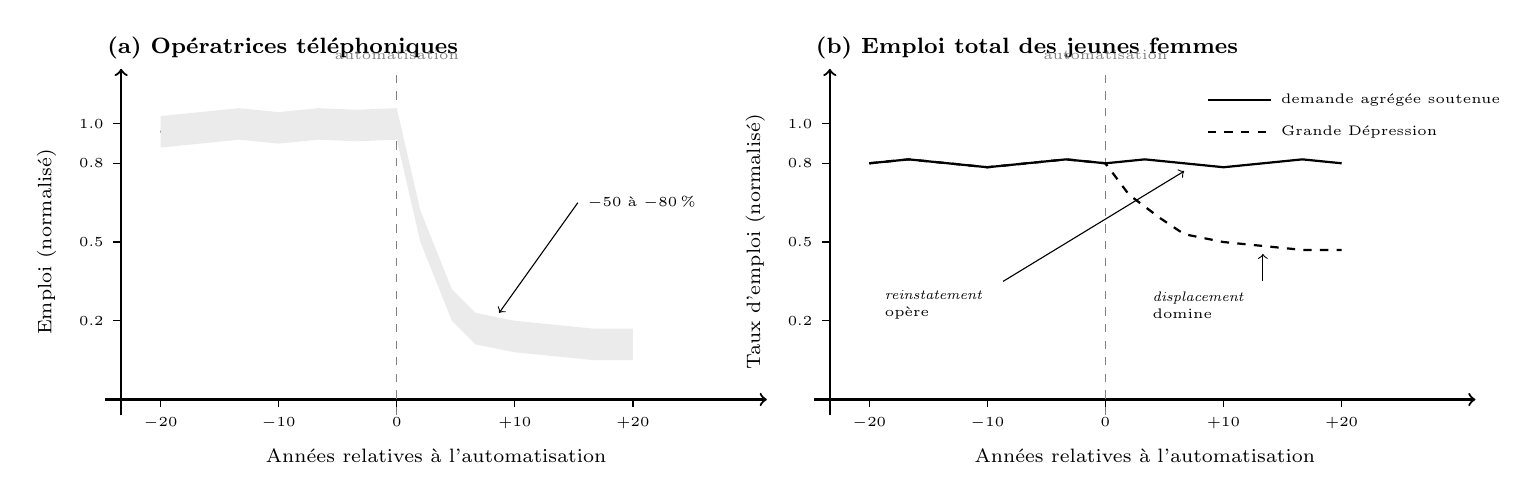
\begin{tikzpicture}
\begin{scope}[xshift=0cm]
  % Panel (a) — Opératrices
  \node[anchor=south west, font=\footnotesize\bfseries] at (-0.3,4.2) {(a) Opératrices téléphoniques};
  
  % Axes
  \draw[->, thick] (-0.2,0) -- (8.2,0) node[right, font=\scriptsize] {};
  \draw[->, thick] (0,-0.2) -- (0,4.2);
  
  % Labels axes
  \node[font=\scriptsize, below] at (4,-0.5) {Années relatives à l'automatisation};
  \node[font=\scriptsize, rotate=90, above] at (-0.7,2) {Emploi (normalisé)};
  
  % Tick marks x
  \foreach \x/\lab in {0.5/$-20$, 2/$-10$, 3.5/$0$, 5/$+10$, 6.5/$+20$} {
    \draw (\x,0) -- (\x,-0.1) node[below, font=\tiny] {\lab};
  }
  
  % Tick marks y
  \draw (0,1) -- (-0.1,1) node[left, font=\tiny] {0.2};
  \draw (0,2) -- (-0.1,2) node[left, font=\tiny] {0.5};
  \draw (0,3) -- (-0.1,3) node[left, font=\tiny] {0.8};
  \draw (0,3.5) -- (-0.1,3.5) node[left, font=\tiny] {1.0};
  
  % Cutover line
  \draw[dashed, gray] (3.5,-0.2) -- (3.5,4.2);
  \node[font=\tiny, gray, above] at (3.5,4.2) {automatisation};
  
  % Pre-cutover: flat at ~3.5
  \draw[thick, black] (0.5,3.4) -- (1,3.45) -- (1.5,3.5) -- (2,3.45) -- (2.5,3.5) -- (3,3.48) -- (3.5,3.5);
  
  % Post-cutover: sharp drop to ~1, then stays low
  \draw[thick, black] (3.5,3.5) -- (3.8,2.2) -- (4.2,1.2) -- (4.5,0.9) -- (5,0.8) -- (5.5,0.75) -- (6,0.7) -- (6.5,0.7);
  
  % Annotation
  \draw[<-, thin] (4.8,1.1) -- (5.8,2.5) node[right, font=\tiny, text width=2cm] {$-50$ à $-80\,\%$};
  
  % Confidence band (very light)
  \fill[black!8] (0.5,3.2) -- (1,3.25) -- (1.5,3.3) -- (2,3.25) -- (2.5,3.3) -- (3,3.28) -- (3.5,3.3) -- (3.5,3.7) -- (3,3.68) -- (2.5,3.7) -- (2,3.65) -- (1.5,3.7) -- (1,3.65) -- (0.5,3.6) -- cycle;
  \fill[black!8] (3.5,3.3) -- (3.8,2.0) -- (4.2,1.0) -- (4.5,0.7) -- (5,0.6) -- (5.5,0.55) -- (6,0.5) -- (6.5,0.5) -- (6.5,0.9) -- (6,0.9) -- (5.5,0.95) -- (5,1.0) -- (4.5,1.1) -- (4.2,1.4) -- (3.8,2.4) -- (3.5,3.7) -- cycle;
\end{scope}

\begin{scope}[xshift=9cm]
  % Panel (b) — Emploi total
  \node[anchor=south west, font=\footnotesize\bfseries] at (-0.3,4.2) {(b) Emploi total des jeunes femmes};
  
  % Axes
  \draw[->, thick] (-0.2,0) -- (8.2,0);
  \draw[->, thick] (0,-0.2) -- (0,4.2);
  
  % Labels
  \node[font=\scriptsize, below] at (4,-0.5) {Années relatives à l'automatisation};
  \node[font=\scriptsize, rotate=90, above] at (-0.7,2) {Taux d'emploi (normalisé)};
  
  % Tick marks x
  \foreach \x/\lab in {0.5/$-20$, 2/$-10$, 3.5/$0$, 5/$+10$, 6.5/$+20$} {
    \draw (\x,0) -- (\x,-0.1) node[below, font=\tiny] {\lab};
  }
  
  % Tick marks y
  \draw (0,1) -- (-0.1,1) node[left, font=\tiny] {0.2};
  \draw (0,2) -- (-0.1,2) node[left, font=\tiny] {0.5};
  \draw (0,3) -- (-0.1,3) node[left, font=\tiny] {0.8};
  \draw (0,3.5) -- (-0.1,3.5) node[left, font=\tiny] {1.0};
  
  % Cutover line
  \draw[dashed, gray] (3.5,-0.2) -- (3.5,4.2);
  \node[font=\tiny, gray, above] at (3.5,4.2) {automatisation};
  
  % Solid line: employment stays flat (normal conditions)
  \draw[thick, black] (0.5,3.0) -- (1,3.05) -- (1.5,3.0) -- (2,2.95) -- (2.5,3.0) -- (3,3.05) -- (3.5,3.0) -- (4,3.05) -- (4.5,3.0) -- (5,2.95) -- (5.5,3.0) -- (6,3.05) -- (6.5,3.0);
  
  % Dashed line: Depression cities — drops after cutover
  \draw[thick, black, dashed] (0.5,3.0) -- (1,3.05) -- (1.5,3.0) -- (2,2.95) -- (2.5,3.0) -- (3,3.05) -- (3.5,3.0) -- (3.8,2.6) -- (4.2,2.3) -- (4.5,2.1) -- (5,2.0) -- (5.5,1.95) -- (6,1.9) -- (6.5,1.9);
  
  % Legend
  \draw[thick, black] (4.8,3.8) -- (5.6,3.8) node[right, font=\tiny] {demande agrégée soutenue};
  \draw[thick, black, dashed] (4.8,3.4) -- (5.6,3.4) node[right, font=\tiny] {Grande Dépression};
  
  % Annotation
  \node[font=\tiny, text width=2.2cm, align=left] at (1.8,1.2) {\emph{reinstatement}\\opère};
  \draw[->, thin] (2.2,1.5) -- (4.5,2.9);
  
  \node[font=\tiny, text width=2.2cm, align=left] at (5.2,1.2) {\emph{displacement}\\domine};
  \draw[->, thin] (5.5,1.5) -- (5.5,1.85);
\end{scope}
\end{tikzpicture}

\caption[Automatisation de la commutation téléphonique~: displacement et reinstatement]{Représentation stylisée du résultat de \textcite{feigenbaum_answering_2024}. Panel~(a)~: l'emploi des opératrices chute de 50 à 80\,\% après l'automatisation. Panel~(b)~: le taux d'emploi total des jeunes femmes reste stable dans les villes à demande agrégée soutenue (trait plein), mais baisse dans les villes frappées par la Grande Dépression (trait pointillé). La compensation opère entre cohortes, pas au sein d'une cohorte~: les incumbents perdent~; les entrantes se réallouent. Source~: construction de l'auteur d'après \textcite{feigenbaum_answering_2024}.}
\label{fig:feigenbaum-stylized}
\end{figure}


Le résultat porte une conditionnalité que la formulation standard du cadre \emph{task-based} ne met pas en avant. Dans les villes frappées par la Grande Dépression, l'automatisation réduit l'emploi sans le compenser~: le \emph{reinstatement} ne se produit pas. La demande agrégée est une condition nécessaire pour que la boucle auto-correctrice opère. Cette conditionnalité n'est pas un détail empirique~--- elle modifie la portée du mécanisme. Le cadre d'\textcite{acemoglu_race_2018} traite le \emph{reinstatement} comme un processus endogène au marché du travail~: de nouvelles tâches émergent parce que le travail est moins cher dans les tâches non automatisées. \textcite{feigenbaum_answering_2024} montrent que ce processus est conditionnel à un facteur exogène au marché du travail~--- la demande agrégée~--- ce qui le rend plus fragile que le cadre théorique ne le suggère.

La régularité se retrouve dans les autres cas du chapitre~1, sans identification causale mais avec une convergence des observations. La calculatrice mécanique dans les bureaux d'assurance (section~\ref{sec:calculating}) restructure le travail sans le supprimer~: \textcite{reinstaller_market_2001} documente une corrélation de 0,921 entre le stock de capital de bureau et l'emploi de bureau aux États-Unis entre 1870 et 1940. La tabulatrice au \emph{Nautical Almanac} remplace les calculateurs qualifiés par des opératrices moins payées et plus étroitement supervisées~--- \textcite{davies_womans_1982} et \textcite{daston_calculation_2018} documentent la même compression salariale par féminisation dans les deux cas. Dans chaque cas, la mécanisation réorganise le travail au lieu de le remplacer. Mais ces cas n'identifient pas les conditions de ce résultat~; seul Feigenbaum et Gross isolent la demande agrégée comme condition nécessaire.

\textcite{autor_expertise_2025} apportent une mise à jour qui modifie la structure du cadre. Ils montrent que la distinction routine/non-routine, qui structurait le cadre depuis \textcite{autor_skill_2003}, est supplantée par la distinction expertise/non-expertise~: ce qui protège le travailleur de l'automatisation n'est plus le caractère non-routinier de sa tâche mais la profondeur de son expertise spécifique. Le résultat est empirique~--- fondé sur l'analyse de la croissance des catégories professionnelles aux États-Unis~--- et modifie les prédictions du cadre pour la période contemporaine, où les modèles de langage automatisent des tâches cognitives non-routinières qui étaient le refuge du travail qualifié dans le cadre antérieur.


\paragraph{Hypothèse H-D3.1} \emph{La transformation du travail par la technique informationnelle obéit au mécanisme displacement-reinstatement du cadre \emph{task-based}, mais l'effet net agrégé dépend de deux conditions exogènes à ce cadre : la configuration du reinstatement parmi les trois variantes d'\textcite{acemoglu_building_2026}~--- \emph{labor-augmenting}, \emph{expertise-leveling}, \emph{new task-creating}~--- qui détermine le partage de la valeur ajoutée ; et le niveau de la demande agrégée, qui détermine si la création de tâches nouvelles peut effectivement absorber le travail déplacé. Quand la demande agrégée fait défaut, le reinstatement ne se produit pas et le déplacement reste sans compensation.} Cette double conditionnalité distingue le mécanisme de la boucle auto-correctrice strictement endogène du cadre d'\textcite{acemoglu_race_2018} ; le chapitre~\ref{ch:imaclim} devra spécifier la configuration du reinstatement comme paramètre de scénario plutôt que comme constante calibrée.

\paragraph{Les compétences comme condition de la forme technique}

Le deuxième mécanisme renverse la direction causale~: ce n'est pas la technique qui transforme le travail, c'est le stock de compétences qui conditionne la forme de la technique adoptée.

\textcite{cohen_absorptive_1990} ont formalisé un mécanisme apparenté au niveau de la firme sous le nom d'\emph{absorptive capacity}~: la capacité d'une organisation à reconnaître, assimiler et exploiter une connaissance externe dépend de son stock de compétences préalable. Le concept est issu de la théorie évolutionniste de la firme \parencite{nelson_winter_1982} et porte sur la R\&D, pas sur l'ICT. Mais son implication structurelle se transpose~: si l'adoption d'une technique exige des compétences spécifiques, et si ces compétences ne sont pas immédiatement disponibles, la vitesse de diffusion est contrainte par le stock de capital humain, pas par le prix du capital physique.

\textcite{david_dynamo_1990} documente le même phénomène par la voie de l'histoire économique~: la diffusion de l'électricité dans l'industrie américaine a pris quarante ans non par défaut technique mais parce que la réorganisation du processus de production~--- passer du système à arbre de transmission au système à moteur individuel~--- exigeait une reconception complète des usines, que les ingénieurs formés dans l'ancien système ne savaient pas faire. \textcite{bresnahan_information_2002} formalisent le coût de cette reconception sous le nom d'\emph{investissements organisationnels complémentaires}~: l'investissement en ICT n'est productif que s'il s'accompagne d'investissements en formation, réorganisation des processus et décentralisation des décisions, dont le coût est du même ordre de grandeur que l'investissement technique lui-même.

Le chapitre~1 fournit deux cas indépendants de ce mécanisme. L'arbitrage Morse/Wheatstone (section~\ref{sec:telegraph}) est un cas où la disponibilité de compétences formables sélectionne le design technique qui prévaut~--- un arbitrage entre capital physique (cinq fils) et capital humain (un opérateur formé au code). Le sémaphore français est un cas inverse~: l'indisponibilité de compétences nouvelles déforme la technique adoptée~--- l'administration fait construire un appareil qui reproduit les gestes de l'ancien système plutôt que de requalifier les opérateurs. Le métier Jacquard illustre une troisième configuration~: les cartes perforées encodent le savoir-faire des tireurs de lacs dans un support matériel, ce qui rend le savoir-faire reproductible mais aussi appropriable~--- les tisserands luddites de 1811--1816 ne détruisaient pas des machines à vapeur mais des machines à information.

La condition d'activation du mécanisme est le degré de spécificité des compétences requises par la nouvelle technique. Quand les compétences sont génériques et transférables, la diffusion est rapide et la forme de la technique n'est pas contrainte. Quand les compétences sont spécifiques~--- au sens de \textcite{williamson_economic_1985}, c'est-à-dire qu'elles perdent de la valeur hors de la relation dans laquelle elles ont été constituées~--- la diffusion est lente et la forme de la technique est déformée par le stock en place.

Ce mécanisme n'a pas de nom unique dans la littérature, parce que les trois traditions qui y contribuent~--- l'\emph{absorptive capacity} de Cohen et Levinthal, les systèmes nationaux d'innovation de \textcite{lundvall_national_1992}, et les \emph{skill bottlenecks} de \textcite{rosenberg_technology_1972}~--- ne se citent pas beaucoup entre elles. Le pont avec l'ICT est surtout dans des rapports institutionnels (OCDE, Banque mondiale) plutôt que dans la littérature académique.


\paragraph{Hypothèse H-D3.2} \emph{Le stock de compétences pré-existant conditionne la forme de la technique informationnelle adoptée, et non seulement son rythme de diffusion. Quand les compétences requises sont spécifiques au sens de \textcite{williamson_economic_1985} et que leur constitution exige un investissement organisationnel comparable à l'investissement technique lui-même \parencite{bresnahan_information_2002}, le design technique qui prévaut n'est pas celui qui maximiserait la performance abstraite mais celui qui est compatible avec le stock de compétences local, quitte à dégrader la technique adoptée. Quand les compétences sont génériques et transférables, la forme de la technique n'est pas contrainte par le stock.} La direction causale est inversée par rapport au cadre \emph{task-based} : c'est ici le travail qui sélectionne la technique, pas l'inverse. L'instanciation la plus pure documentée au chapitre~1 est l'arbitrage Morse/Wheatstone, où la disponibilité d'opérateurs formables au code détermine quel design des deux l'emporte.

\paragraph{Le travail de conception comme produit de la mécanisation}

Le troisième mécanisme porte sur un type de travail que la mécanisation crée au lieu de le réduire. Dans les trois cas du chapitre~1 où une organisation mécanise le traitement de l'information, un travail intellectuel de conception apparaît qui n'existait pas avant la mécanisation\footnote{Dans la taxonomie d'\textcite{acemoglu_building_2026}, ce mécanisme correspond à la catégorie \emph{new task-creating}~: la mécanisation crée de la demande pour une expertise qui n'existait pas, ce qui augmente la part du travail dans la valeur ajoutée. L'identification par induction historique (trois cas indépendants sur cent cinquante ans) et l'ancrage formel dans le cadre \emph{task-based} sont deux voies indépendantes qui convergent vers la même proposition, ce qui en fait un cas de consilience au sens du protocole multi-école du présent chapitre.}.

McCallum, sur l'\emph{Erie Railroad} (section~\ref{subsec:railroad}), déploie six formes informationnelles dont le télégraphe n'est que la quatrième~; les cinq autres~--- le \emph{rule book}, la hiérarchie managériale, le reporting, la comptabilité analytique, la standardisation~--- sont du travail de conception codifié. Au \emph{Nautical Almanac}, Comrie estime que vingt à trente pour cent du temps du surintendant sont consacrés à concevoir les séquences dans lesquelles humains et machines s'articulent~--- l'\emph{analytical intelligence} de \textcite{daston_calculation_2018}. Bolle, au PLM (section~\ref{sec:mechanography}), formule la même leçon dans une devise~: \og \emph{d'abord organiser, ensuite mécaniser}\fg{}. Dans ces trois cas, la machine est un composant d'un système dont le reste est du travail qualifié de conception.

\textcite{bresnahan_information_2002} mesurent le coût de ce travail complémentaire~: l'investissement organisationnel nécessaire pour rendre l'ICT productive est du même ordre de grandeur que l'investissement technique. \textcite{david_dynamo_1990} mesure le délai~: quarante ans pour que l'électricité produise des gains de productivité mesurables, parce que la reconception des processus prend une génération. Mais ni Bresnahan ni David ne formalisent le lien entre les deux observations~: le coût de réorganisation est essentiellement un coût de travail qualifié de conception, et ce travail est un input permanent du système, pas un coût transitoire d'ajustement.

La condition d'activation est la complexité de l'interface humain-machine. Quand la machine est un outil isolé~--- la calculatrice mécanique~--- le travail de conception est minimal. Quand la machine est un composant d'un système~--- le télégraphe dans le réseau ferroviaire, la tabulatrice dans la chaîne mécanographique~--- le travail de conception est proportionnel à la complexité du système. Ce gradient fait écho à celui de la dimension~3 (isolé/intégré)~: le capital intégré exige du travail de conception intégré.

Le caractère permanent ou transitoire de ce coût reste ouvert. David~(1990) le traite comme transitoire~: une fois les usines reconçues, le coût disparaît. Mais le cas de McCallum suggère le contraire~: les huit clercs qui traitent l'information entrante et sortante de la division ne sont pas un coût de transition~--- ils sont un coût d'exploitation permanent du système informationnel. Si le ratio travail de conception / travail d'exécution augmente avec chaque vague de mécanisation, le coût est structurel, pas transitoire.


\paragraph{Hypothèse H-D3.3} \emph{La mécanisation d'une fonction informationnelle crée un travail intellectuel de conception qui ne préexistait pas~--- il porte sur les interfaces, les séquences, les règles, et son coût est, selon \textcite{bresnahan_information_2002}, du même ordre de grandeur que l'investissement technique. Le volume de ce travail croît avec la \emph{complexité de coordination} du système organisationnel, définie par la diversité des configurations à traiter, leur degré d'interdépendance, et l'exigence de propriétés systémiques telles que la sécurité, la cohérence ou la traçabilité. Ce gradient est distinct de celui d'intégration technique du capital (H-D2.3), bien que corrélé empiriquement : le télégraphe de McCallum sur l'\emph{Erie Railroad} illustre une complexité de coordination maximale avec une intégration technique faible, et des cas inverses existent.} La question de savoir si ce coût est transitoire au sens de \textcite{david_dynamo_1990} ou structurel et croissant à chaque vague de mécanisation reste ouverte ; le chapitre~\ref{ch:imaclim} devra trancher par calibration sur les données contemporaines.

\subsubsection{Observations non formalisées}

Deux observations du chapitre~1 ne satisfont pas les critères d'un mécanisme au sens du protocole~--- elles reposent chacune sur un seul cas développé~--- mais posent des questions que la littérature contemporaine instruit.

La première est la résistance par le savoir tacite. L'automatisation de la commutation téléphonique a pris soixante ans, de Strowger (1891) à la généralisation (section~\ref{sec:telephone}). \textcite{feigenbaum_organizational_2024} montrent que l'explication ne réside ni dans la résistance syndicale ni dans un défaut technique, mais dans le fait que la commutation portait un savoir organisationnel implicite~--- facturation, réclamations, renseignements, urgences~--- dont l'extraction exigeait la reconfiguration de l'ensemble du système Bell. C'est une tâche \emph{intégrale} au sens de \textcite{ulrich_role_1995}. \textcite{autor_polanyi_2014} a nommé ce phénomène le \og paradoxe de Polanyi\fg{}~: les tâches que les humains exécutent sans savoir les formuler explicitement résistent à la programmation. L'IA générative, qui procède par pattern-matching statistique plutôt que par codification explicite, pourrait contourner ce paradoxe~--- mais les résultats empiriques sur ce point sont encore fragiles.

La seconde observation est le pattern biographique de mobilité inter-paradigmatique. Edison transpose la maîtrise des circuits du télégraphe vers l'électrification (section~\ref{sec:electrification}). Siemens transpose la connaissance des signaux de l'artillerie vers le télégraphe (section~\ref{sec:telegraph}). Shannon connecte l'algèbre de Boole au circuit de commutation. La récurrence suggère que la diffusion des paradigmes techniques passe en partie par la mobilité des personnes. Mais c'est une observation biographique, pas un mécanisme~: le chapitre n'a pas les moyens de déterminer si ce canal est quantitativement significatif.


\subsubsection{Test contemporain}

\paragraph{Évidence historique}

Le matériau du chapitre~1 hiérarchisé selon le protocole donne un résultat net. Un seul mécanisme est causalement identifié~: la restructuration conditionnée par la demande agrégée, par l'estimation de \textcite{feigenbaum_answering_2024} sur la commutation téléphonique. Trois régularités sont reproductibles sans identification causale~: la restructuration sans suppression (calculatrice, \emph{Nautical Almanac}, téléphone~--- quatre cas sur cent cinquante ans), la féminisation et la compression salariale dans le travail de calcul \parencite{davies_womans_1982,strom_tipping_1992,daston_calculation_2018}, et la migration du goulot cognitif vers le haut (Prony, Comrie, Bolle, McCallum~--- le travail de conception augmente avec la mécanisation). Les observations singulières~--- le Calenberg comme coût corporel du calcul, la recommandation genrée de Comrie au \emph{Nautical Almanac}, les ENIAC Six~--- ne sont pas mobilisées comme preuve mais comme illustration de la diversité des configurations.

\paragraph{Évidence contemporaine~: études causales}

Les études causales \emph{cross-country} confirment le premier mécanisme et en précisent les contours. \textcite{michaels_has_2014}, sur onze pays et vingt-cinq ans de données EU~KLEMS, montrent que l'intensification de l'ICT augmente la demande relative de travail qualifié et réduit celle du travail intermédiaire~--- le pattern de polarisation que le cadre \emph{task-based} prédit. \textcite{akerman_skill_2015}, exploitant le déploiement géographique du haut débit en Norvège comme instrument, montrent que le broadband augmente les salaires des qualifiés et réduit ceux des non-qualifiés au sein des mêmes firmes~: la complémentarité technologie-qualification opère à l'intérieur de la firme, pas seulement entre firmes. \textcite{dauth_adjusting_2021}, sur les robots en Allemagne, trouvent que la destruction d'emplois manufacturiers ne se traduit pas en hausse du chômage~: la réallocation opère par mobilité intra-firme vers des tâches non manufacturières. \textcite{cette_icl_2021}, sur données de firmes françaises, montrent que la numérisation augmente la productivité mais réduit la part du travail au niveau de la firme.

L'ensemble dessine un tableau cohérent avec le premier mécanisme~: la technique restructure, le \emph{reinstatement} opère, mais l'ajustement est inégalement distribué. Les données macroéconomiques agrégées ne montrent pas de relation robuste entre investissement ICT et part du travail au niveau national~--- \textcite{autor_salomons_2018} montrent que la productivité réduit la part du travail \emph{within-industry} mais que les \emph{spillovers cross-industry} compensent partiellement. Le signal est dans la composition sectorielle et inter-firmes, pas dans l'agr\'egat.

\paragraph{\'Evidence contemporaine~: l'ICT non-IA}

Les trois m\'ecanismes discriminent \'egalement dans les formes contemporaines d'ICT qui ne rel\`event pas de l'IA g\'en\'erative. Le passage du logiciel sous licence perp\'etuelle au mod\`ele SaaS par abonnement~--- document\'e dans la dimension~2 (H-D2.2) comme transformation du mode d'appropriation du capital~--- restructure les comp\'etences requises~: l'administrateur \emph{on-premise}, dont le savoir-faire porte sur la configuration mat\'erielle locale, c\`ede la place \`a l'architecte cloud, dont les comp\'etences portent sur l'orchestration de services distribu\'es. C'est un cas contemporain de H-D3.2~: la forme de la technique adopt\'ee est conditionn\'ee par la disponibilit\'e de comp\'etences sp\'ecifiques, et la transition est ralentie par le co\^ut de requalification.

L'\'ecosyst\`eme CUDA de Nvidia (dimension~2, H-D2.3) illustre le m\'ecanisme inverse~: quatre millions de d\'eveloppeurs form\'es \`a une plateforme logicielle propri\'etaire constituent un stock de comp\'etences d\'elib\'er\'ement construit par la firme pour verrouiller le march\'e. La sp\'ecificit\'e des comp\'etences n'est pas ici une contrainte exog\`ene~--- elle est un instrument de \emph{design du capital} au sens de H-D2.2, qui op\`ere par le travail.

Les communs num\'eriques~--- Linux, PostgreSQL, Apache, document\'es dans la dimension~2 comme test n\'egatif du mode d'appropriation~--- produisent une forme de travail de conception radicalement diff\'erente de celle que H-D3.3 d\'ecrit dans le cas hi\'erarchique. Le travail de conception existe~--- les mainteneurs, les r\'edacteurs de documentation, les testeurs~--- mais il est distribu\'e entre communaut\'es, souvent non r\'emun\'er\'e par les canaux salariaux standards, et organis\'e par des r\`egles de gouvernance sp\'ecifiques \parencite{benkler_wealth_2006}. La production par les pairs fond\'ee sur les communs (\emph{commons-based peer production}) est un r\'egime o\`u le travail de conception est permanent et croissant~--- comme le pr\'edit H-D3.3~--- mais o\`u la r\'epartition de ce travail ne passe pas par le march\'e du travail.

Enfin, le mobile banking en Afrique subsaharienne~--- dont M-Pesa est l'arch\'etype~--- cr\'ee des cat\'egories de travail nouvelles (agents de \emph{mobile money}, techniciens de r\'eseau) qui n'existaient pas avant le d\'eploiement de l'infrastructure. C'est du \emph{new work} au sens d'\textcite{autor_new_2024}, dans un contexte o\`u l'IA ne joue aucun r\^ole~: la cr\'eation de t\^aches nouvelles par l'ICT n'est pas un ph\'enom\`ene propre \`a l'IA.

Ces cas montrent que les trois m\'ecanismes op\`erent dans le r\'egime ICT contemporain avant l'IA~: la restructuration conditionnelle (H-D3.1) dans les robots et le broadband, la conditionnalit\'e par les comp\'etences (H-D3.2) dans la transition cloud et l'\'ecosyst\`eme CUDA, le travail de conception croissant (H-D3.3) dans les communs et le mobile banking. L'IA g\'en\'erative n'est donc pas le terrain o\`u ces m\'ecanismes apparaissent~--- c'est le terrain o\`u ils pourraient cesser d'op\'erer.

\paragraph{Évidence contemporaine~: l'IA générative}

Trois résultats récents modifient le diagnostic.

\textcite{eloundou_gpts_2023} estiment, par une combinaison de jugement expert et de tests sur les API de GPT, qu'environ 80~\% des travailleurs américains ont au moins 10~\% de leurs tâches exposées aux modèles de langage, et qu'environ 19~\% ont au moins 50~\% de leurs tâches exposées. Le résultat est que l'exposition est plus élevée pour les qualifiés que pour les non-qualifiés~--- l'inverse du pattern ICT historique. Si le cadre \emph{task-based} s'applique, cela signifie que l'IA générative déplace le \emph{displacement} vers le haut de la distribution des qualifications, là où le \emph{reinstatement} opérait dans les vagues précédentes.

\textcite{brynjolfsson_generative_2023} montrent, dans un essai contrôlé randomisé sur plus de cinq mille agents de service client, que l'accès à un assistant IA augmente la productivité de 14~\% en moyenne~--- mais que l'effet est concentré sur les travailleurs les moins expérimentés, dont la productivité augmente de 34~\%, tandis que les plus expérimentés ne bénéficient que d'un gain modeste. L'IA comprime la distribution des productivités vers le haut~: elle substitue l'expérience par le modèle. La taxonomie d'\textcite{acemoglu_building_2026} pose une question que ce résultat, à lui seul, ne tranche pas~: l'assistant IA des agents de service client est-il une technologie \emph{labor-augmenting} (les agents font mieux les mêmes tâches), \emph{expertise-leveling} (les novices accèdent à des tâches qui étaient celles des experts) ou \emph{new task-creating} (des tâches inédites deviennent possibles)~? La hausse de productivité des novices est compatible avec les deux premières lectures~; elle n'est compatible avec la troisième que si les agents accomplissent désormais des tâches qu'aucun agent n'exécutait auparavant, ce que le dispositif de \textcite{brynjolfsson_generative_2023} ne mesure pas. La nature du \emph{reinstatement} observé reste une question ouverte~--- ce qui justifie d'en faire un paramètre de scénario au chapitre~\ref{ch:imaclim} plutôt qu'une constante calibrée.

\textcite{brynjolfsson_canaries_2025}, sur des données ADP couvrant environ vingt-six millions de travailleurs américains, montrent que l'emploi des 22--25~ans dans les occupations exposées à l'IA a baissé d'environ vingt pour cent depuis fin 2022, tandis que les travailleurs plus âgés dans les mêmes occupations ne sont pas affectés. Le parallèle avec \textcite{feigenbaum_answering_2024} est direct~: dans les deux cas, ce sont les entrants (jeunes, \emph{entry-level}) qui subissent le choc, tandis que les incumbents (expérimentés) sont retenus. Mais la période d'observation est courte~--- trois ans~--- et les auteurs ne peuvent pas isoler l'effet IA des autres changements macroéconomiques de la période.

\paragraph{Le \emph{so-so automation} et le \emph{productivity bandwagon}}

\textcite{acemoglu_power_2023} posent un cadre interprétatif qui articule les résultats précédents. Le \emph{so-so automation} désigne l'automatisation qui déplace le travailleur sans gain de productivité suffisant pour enclencher le \emph{reinstatement}~: les caisses automatiques qui n'améliorent pas le service, les chatbots qui perdent l'intelligence situationnelle du représentant humain, les algorithmes de diagnostic qui échouent là où le jugement contextuel du praticien réussissait~--- \textcite{hinton_2016} prédisait en 2016 la disparition des radiologistes en cinq ans~; la demande a augmenté depuis, parce que le diagnostic exige un jugement situationnel et social que l'algorithme ne réplique pas. Le cas Toyota/GM-Fremont est l'instanciation la plus propre de la distinction. GM Fremont ferme en 1982 pour basse productivité et conflits sociaux. Toyota rouvre la même usine avec les mêmes travailleurs et le même syndicat, mais combine machines avancées avec formation, flexibilité et initiative~; la productivité atteint les niveaux japonais. Tesla refait l'erreur inverse trente ans plus tard en automatisant chaque étape de la production~: les coûts explosent, les délais s'accumulent, et Musk reconnaît que \og \emph{excessive automation at Tesla was a mistake. Humans are underrated}\fg{}. C'est le test empirique le plus direct du troisième mécanisme~: l'automatisation substitutive échoue quand elle détruit le travail de conception que le système exige.

Le \emph{productivity bandwagon}~--- l'idée que les gains de productivité se diffusent automatiquement en salaires et en emploi~--- est la condition macro sous laquelle le \emph{reinstatement} opère. \textcite{acemoglu_power_2023} montrent, sur les séries longues américaines, que le bandwagon ne fonctionne que sous trois conditions~: concurrence suffisante entre employeurs, pouvoir de négociation des travailleurs, et gains de productivité réels. Entre 1949 et 1973, les trois conditions tiennent~: les salaires réels médians croissent de 2,5~\% par an, au même rythme que la productivité. Après 1980, les trois s'affaiblissent~: les salaires médians ne croissent plus que de 0,45~\% par an tandis que la productivité continue à 1,5~\%~; les hommes sans diplôme voient leurs salaires baisser~; la part du top~1~\% remonte de 10~\% à 19~\% du revenu national entre 1980 et 2019~; la part du travail passe de 67--70~\% à moins de 60~\%. Ce découplage salaires/productivité est le fait macro qui encadre le fait stylisé de cette dimension~: la boucle auto-correctrice du cadre \emph{task-based} est conditionnelle à des paramètres institutionnels que la littérature formelle d'\textcite{acemoglu_race_2018} ne modélise pas explicitement.


\subsubsection{Fait stylisé}

Le rapport entre les techniques de l'information et le travail est multidirectionnel~: la technique restructure le travail par le \emph{displacement} et le \emph{reinstatement} (premier mécanisme), mais le stock de compétences conditionne la forme de la technique adoptée (deuxième mécanisme) et la mécanisation crée un travail de conception qui ne préexistait pas (troisième mécanisme). Le résultat net sur l'emploi dépend d'une condition exogène au marché du travail~--- la demande agrégée~--- ce qui rend la boucle auto-correctrice du cadre \emph{task-based} plus fragile que sa formulation théorique ne le suggère.

Le diagnostic historique~--- la restructuration l'emporte sur la suppression, à condition que la demande agrégée soutienne le \emph{reinstatement}~--- tient encore dans les données contemporaines sur l'ICT. L'arrivée de l'IA générative introduit deux perturbations dont les effets ne sont pas encore mesurables avec la même précision. La première est l'automatisation des tâches cognitives non-routinières, qui ferme le refuge du travail qualifié que le cadre \emph{task-based} lui assignait~: l'expertise, et non plus le caractère non-routinier, devient la variable discriminante \parencite{autor_expertise_2025}. La seconde est le croisement avec la dimension~3~: si le coût de l'automatisation est déterminé par le prix de l'énergie et du capital computationnel plutôt que par le prix relatif du travail, la boucle auto-correctrice d'\textcite{acemoglu_race_2018}~--- dans laquelle la baisse du prix du travail rend le \emph{reinstatement} plus attractif que le \emph{displacement}~--- perd son ancrage. Cette hypothèse croise les dimensions~3 (capital hybride) et~0-TER (énergie)~; elle est posée ici, pas testée. Le chapitre~4 devra déterminer si elle tient dans le modèle.

La configuration du reinstatement et le niveau de demande agrégée peuvent être traités comme paramètres de scénario, à condition que le cadre de modélisation retenu permette de faire varier le partage de la valeur ajoutée indépendamment de la productivité totale des facteurs~; cette condition technique est examinée au chapitre~\ref{ch:imaclim}. La double conditionnalité transforme un automatisme du cadre task-based standard en variable de scénario, ce qui change qualitativement la trajectoire de la part du travail et donc la composition de la demande finale.

\wip{\textcolor{teal}{Refs Aubouin non encore intégrées~: Goldin \& Katz 1998 (\emph{QJE}) --- complémentarité technologie-qualification longue durée. Karabarbounis \& Neiman 2014 (\emph{QJE}) --- baisse part du travail. Gutiérrez \& Piton 2020 --- nuance housing. Acemoglu \& Restrepo 2017 --- stagnation séculaire + automatisation.}}


% =============================================================================
\clearpage
\subsection{Rendements d'échelle et externalités de réseau}\label{sec:d4-reseau}

Dans certains marchés, l'adoption d'un bien par un agent modifie la valeur ou le coût du même bien pour d'autres agents. L'organisation industrielle étudie ces interdépendances d'adoption~--- externalités de réseau directes et indirectes, rendements d'échelle tirés par les données, effets informationnels~--- et leurs conséquences sur la structure de marché. Cette dimension examine par quels canaux ces interdépendances opèrent dans les marchés de biens informationnels, et à quelles conditions elles déterminent la structure de marché qui en résulte.


\subsubsection{Le champ}

Certains marchés numériques sont des quasi-monopoles~: Google détient 91\,\% du marché mondial de la recherche en ligne en 2024\footnote{Source~: StatCounter Global Stats, décembre 2024.}, Meta contrôle environ 75\,\% du temps passé sur les réseaux sociaux en Occident. D'autres marchés numériques restent fragmentés~: le commerce en ligne, la fintech, les services cloud aux PME. Cette variance est le problème que cette section ouvre. Elle ne peut pas s'expliquer par les coûts fixes seuls --- l'analyse des propriétés du bien informationnel a montré que le coût marginal nul et le coût fixe élevé sont communs à \emph{tous} les biens informationnels, concentrés ou non. Elle ne peut pas non plus s'expliquer par la forme du capital --- l'analyse du capital informationnel a montré que le mode d'appropriation (vente vs.\ location avec consommable exclusif) est un déterminant de la concentration, mais il opère par un autre canal. La question propre à cette section est~: à quelles conditions les \emph{externalités entre agents} --- le fait que l'adoption d'un bien par un agent modifie la valeur ou le coût pour d'autres agents --- produisent-elles le basculement (\emph{tipping}) vers le monopole plutôt que la coexistence de plusieurs acteurs~?

\paragraph{Contributions propres de la section}
L'apport de cette section est double. D'abord, une typologie en quatre types d'externalités différenciées par le lieu de la boucle de rétroaction~--- demande, offre, cognition~--- qui empêche le collapsus standard selon lequel les effets de réseau produisent mécaniquement la concentration. Ensuite, un test négatif explicite~--- l'internet banking, qui déconcentre~--- qui délimite le domaine de validité de la boucle données-qualité de H-D4.2 et distingue méthodologiquement la portabilité du partage des données comme instruments aux effets de structure opposés.

\subsubsection{Quatre types d'externalités}

Avant d'identifier des mécanismes, il faut distinguer les types d'externalités entre agents que la littérature et le matériau historique font apparaître. Le tableau~\ref{tab:d2-externalites} les présente sous forme de questions simples.

\begin{table}[!ht]
\caption{Quatre types d'externalités entre agents dans les marchés informationnels.}\label{tab:d2-externalites}
\centering\footnotesize
\renewcommand{\arraystretch}{1.25}
\begin{tabularx}{\textwidth}{@{}p{2.2cm}Xp{2.8cm}p{2.8cm}@{}}
\toprule
\textbf{Type} & \textbf{Question simple} & \textbf{Où se situe la boucle} & \textbf{Cas de référence} \\
\midrule
Directe & Mon bien devient-il plus utile quand d'autres l'adoptent~? & Demande~: valeur perçue par l'usager & Téléphone (1880--1920) \\[4pt]
Indirecte croisée & La présence d'usagers d'un côté attire-t-elle des fournisseurs de l'autre côté, et réciproquement~? & Demande croisée~: deux côtés du marché & Consoles de jeux, cartes de crédit \\[4pt]
Data-driven & L'usage génère-t-il des données qui réduisent le coût d'amélioration du produit~? & Offre~: coût d'innovation & Moteurs de recherche, LLMs (depuis GPT-3, 2020) \\[4pt]
Informationnelle & L'observation du choix d'autrui réduit-elle mon incertitude sur la qualité du bien~? & Cognition~: inférence sans interaction & Localisation d'entreprises (Silicon Valley, Silicon Sentier) \\
\bottomrule
\end{tabularx}
\renewcommand{\arraystretch}{1.0}
\end{table}

Ces quatre types ne sont pas des synonymes~: ils diffèrent par le lieu de la boucle de rétroaction (demande, offre, cognition) et par les conditions qui les activent ou les désactivent. Les deux premiers sont classiques dans la littérature d'organisation industrielle depuis \textcite{katz_network_1985} et \textcite{rochet_platform_2003}. Le troisième est identifié et formalisé par \textcite{pruefer_competing_2021}. Le quatrième est distingué des trois premiers par \textcite{vicente_externalites_2002} dans le cadre de l'économie géographique.


\subsubsection{Ce que le matériau révèle}

Quatre régularités se dégagent de la confrontation entre le matériau historique et les données contemporaines. Elles sont posées ici comme des constats observés, avant d'être formalisées comme mécanismes dans la section suivante.

\paragraph{Première régularité~: même époque, même clientèle, résultats opposés.}

Le réseau téléphonique américain bascule vers le monopole entre 1880 et 1920~: AT\&T contrôle plus de 80\,\% des lignes à la fin de cette période, après avoir systématiquement refusé l'interconnexion aux compagnies indépendantes \parencite{beauchamp_invented_2010}. La calculatrice mécanique, vendue aux mêmes grandes organisations à la même époque, ne bascule pas~: le marché compte une centaine de firmes en 1904 \parencite{cortada_before_1993}. Ce qui diffère n'est ni la technologie ni la clientèle~: c'est que le téléphone a des externalités directes fortes (ma ligne n'a de valeur que si d'autres sont connectés), tandis que la calculatrice n'en a aucune (ma machine calcule aussi bien que mon voisin en ait une ou non).

\paragraph{Deuxième régularité~: des externalités de réseau sans basculement.}

Le marché des cartes mémoire flash entre 2003 et 2006 présente des externalités de réseau mesurables~: un format plus répandu facilite le transfert de données entre appareils. Pourtant, plusieurs standards incompatibles (SD, CompactFlash, Memory Stick, xD) coexistent sur toute la période. \textcite{liu_standards_2012} montrent, par régression hédonique sur les prix, que l'existence de lecteurs multi-cartes à faible coût réduit la prime de prix du format dominant. La compatibilité est assurée par le hardware de conversion, pas par la standardisation~: le basculement ne se produit pas parce que le coût de la conversion est inférieur au bénéfice de l'externalité.

\paragraph{Troisième régularité~: même type d'agglomération, stabilité opposée.}

La Silicon Valley est une agglomération de firmes numériques qui persiste à travers les cycles conjoncturels~: le krach de 2001 réduit le nombre de firmes mais ne disperse pas le cluster. Le Silicon Sentier parisien, agglomération similaire formée à la fin des années 1990, s'effondre avec la bulle Internet. \textcite{vicente_externalites_2002} observe que les deux cas diffèrent par le type d'externalité~: la Valley repose sur des interactions réelles (marché du travail partagé, coopérations technologiques, infrastructure commune), le Sentier repose sur l'observation des choix d'autrui (les firmes s'installent parce que d'autres s'installent).

\paragraph{Quatrième régularité~: la numérisation déconcentre un marché.}

L'internet banking, étudié par \textcite{lyons_digital_2024}, a un effet déconcentrant significatif sur le secteur bancaire. Ce résultat est contre-intuitif~: si les externalités de réseau produisent la concentration, la numérisation d'un secteur devrait concentrer, pas disperser. L'hypothèse la plus économe est que la donnée n'est pas l'input principal de la qualité du service bancaire~: la numérisation y agit comme un égaliseur --- elle dévalue les actifs physiques (le réseau d'agences) qui protégeaient les \emph{incumbents} --- plutôt que comme un concentrateur.


\subsubsection{Trois mécanismes}

Les quatre régularités qui précèdent ne s'expliquent pas par un mécanisme unique. Trois canaux causaux distincts permettent d'en rendre compte. Chacun est présenté selon la progression~: observation qui le motive, cadre théorique qui l'éclaire, phénomène contemporain qui le prolonge, formulation et hypothèse.

\paragraph{Premier mécanisme --- Le basculement par coordination anticipative}

\markNEO \markEVO

Le réseau téléphonique américain bascule vers le monopole en une génération. L'analyse historique montre que trois conditions sont réunies~: les externalités directes sont fortes (la valeur d'une ligne croît avec le nombre d'abonnés), les usagers sont en \emph{single-homing} (un abonné n'a qu'une seule ligne), et l'interconnexion est refusée par l'opérateur dominant \parencite{beauchamp_invented_2010}. La calculatrice, qui ne satisfait aucune de ces trois conditions, reste un marché fragmenté. Le contraste suggère que les externalités de réseau ne suffisent pas à produire le basculement~: il faut des conditions structurelles supplémentaires.

Dans une lecture d'organisation industrielle --- par exemple \textcite{katz_network_1985} --- le basculement s'explique par le rôle des anticipations. Les agents ne choisissent pas seulement en fonction de la qualité présente du bien~; ils choisissent en fonction de la taille qu'ils \emph{anticipent} pour le réseau futur. Si une majorité d'agents anticipe qu'un standard va dominer, cette anticipation se réalise d'elle-même~: chacun adopte le standard anticipé, ce qui le fait effectivement dominer. \textcite{arthur_competing_1989} formalise cette dynamique comme un processus à renforcement positif --- un processus où chaque adoption augmente la probabilité de l'adoption suivante\footnote{Arthur modélise le processus comme une urne de Pólya généralisée~: une urne contient des boules de deux couleurs~; à chaque tirage, on ajoute une boule de la couleur tirée. La proportion d'une couleur converge vers 0 ou 1 avec probabilité~1, mais la couleur gagnante dépend des premiers tirages --- c'est le \emph{path dependence}.}. Le résultat ne dépend pas de la supériorité intrinsèque du standard~; il dépend des croyances des agents sur le comportement des autres agents.

Les marchés bifaces ajoutent une couche à ce mécanisme. \textcite{rochet_platform_2003} et \textcite{armstrong_competition_2006} montrent que lorsque les externalités sont indirectes et croisées entre deux côtés d'un marché (usagers et développeurs pour une console, acheteurs et vendeurs pour une place de marché), la plateforme qui les internalise adopte une structure de prix non standard~: un côté est subventionné, l'autre paie. Cette structure de subvention croisée, absente des marchés à externalités directes comme le téléphone, est un instrument supplémentaire de basculement~: la plateforme qui subventionne le bon côté attire la masse critique plus vite que ses concurrentes \parencite{rysman_economics_2009}.

Cependant, le basculement n'est pas une fatalité. Le marché des cartes mémoire flash (deuxième régularité) montre que l'existence de technologies de conversion à faible coût neutralise l'effet de réseau~: quand un lecteur multi-cartes coûte quelques dollars, la taille du réseau d'un format cesse d'être un critère de choix \parencite{liu_standards_2012}. \textcite{jullien_economics_2021} montrent plus généralement que le \emph{multi-homing} --- la possibilité pour l'usager d'être sur plusieurs réseaux simultanément --- empêche le basculement en préservant la valeur de chaque réseau. Les coûts de conversion ne sont pas toujours d'origine technique~: les \emph{egress fees} des hyperscalers cloud et les incompatibilités d'API propriétaires sont des barrières tarifaires délibérées, construites par le design du capital au sens de H-D2.2, qui élèvent le coût de \emph{multi-homing} au-delà de ce que la technologie imposerait.

\paragraph{Hypothèse H-D4.1} \emph{Le basculement par coordination anticipative se produit lorsque trois conditions sont simultanément réunies~: les externalités de réseau sont fortes relativement à la différenciation des préférences, les usagers sont en \emph{single-homing}, et l'interopérabilité entre réseaux est faible. Lorsque l'une de ces conditions tombe --- par exemple par l'existence de technologies de conversion à faible coût --- le basculement ne se produit pas, même en présence d'externalités fortes. Le test de cette hypothèse requiert la comparaison systématique de marchés à externalités fortes avec et sans interopérabilité.}


\paragraph{Deuxième mécanisme --- La boucle données-qualité}

\markNEO \markEVO

La quatrième régularité --- l'internet banking qui déconcentre --- pose un problème. Si les externalités de réseau expliquaient la concentration des marchés numériques, tous les marchés numérisés devraient se concentrer. Or ce n'est pas le cas. Le mécanisme de coordination anticipative (H-D4.1) ne s'applique pas ici~: la banque en ligne n'a pas d'externalités directes fortes. Il faut un autre canal pour expliquer pourquoi certains marchés numériques concentrent (recherche en ligne, réseaux sociaux) et d'autres non (banque, e-commerce de niche).

\textcite{pruefer_competing_2021} identifient et formalisent ce canal. Dans leur modèle, deux firmes se font concurrence par la qualité. Chaque firme accumule des données sur ses usagers --- un sous-produit automatique de l'usage. Ces données réduisent le coût marginal d'amélioration de la qualité. La firme qui a plus de données produit une meilleure qualité à moindre coût, ce qui attire de nouveaux usagers, qui génèrent de nouvelles données. La boucle est côté offre~: même si l'usager se fiche que d'autres utilisent le même service --- aucune externalité de réseau directe ---, le leader gagne parce qu'il est structurellement plus efficace pour innover. Une précision est nécessaire sur la nature de la donnée qui alimente la boucle. \textcite{pruefer_competing_2021} modélisent des données d'usage~--- le sous-produit de l'interaction entre l'usager et le service. Dans le régime des modèles de fondation, le canal dominant est différent~: c'est le corpus d'entraînement~--- des données massives préexistantes (textes, images, code)~--- qui détermine la qualité du modèle de base, et le retour d'usage (RLHF, \emph{fine-tuning}) n'intervient qu'en ajustement fin. Les deux canaux n'activent pas la même boucle~: le premier est un flux renouvelé par l'usage, le second est un stock dont l'accumulation précède le déploiement. La distinction importe parce qu'un stock fini sature là où un flux se renouvelle.

Ce canal se distingue formellement des courbes d'apprentissage classiques. Dans le modèle de \textcite{cabral_learning_1994}, les coûts marginaux convergent vers un plancher~$\bar{c}$~: la firme en retard finit toujours par rattraper la firme dominante, parce que la convergence des coûts est un résultat endogène. Dans le modèle de \textcite{pruefer_competing_2021}, la qualité n'a pas de borne supérieure et l'avantage de coût d'innovation est permanent~; le rattrapage ne se produit pas. Après le basculement, l'innovation stagne des deux côtés~: le leader n'a plus besoin d'innover pour rester seul, et le suiveur ne peut plus se permettre d'investir. \textcite{pruefer_competing_2021} nomment ce résultat un \emph{piège à innovation}.

La condition d'activation est l'exclusivité de la donnée. Si les données utilisateurs sont partagées entre concurrents, les fonctions de coût s'égalisent et l'avantage cumulatif s'effondre~: \textcite{pruefer_competing_2021} établissent que le partage obligatoire des données élimine le basculement. Ce résultat distingue deux instruments de politique de concurrence souvent confondus~: la \emph{portabilité} des données (qui réduit les coûts de migration individuelle) et le \emph{partage} des données (qui égalise les fonctions de coût agrégées). Comme le montre le paradoxe de \textcite{giovannetti_platform_2023}, ces deux instruments peuvent avoir des effets opposés sur la structure de marché --- un point développé dans la confrontation ci-dessous.

Le phénomène contemporain qui rend ce mécanisme central est l'émergence des modèles de fondation à grande échelle depuis GPT-3 \parencite{brown_language_2020}. Epoch~AI documente systématiquement les coûts et les tendances\footnote{Les données citées dans ce paragraphe proviennent de \textcite{cottier_rising_2024} et du \emph{dashboard} Epoch~AI Trends (\url{https://epoch.ai/trends}), consulté en mai~2026.}. Le compute d'entraînement des modèles frontier croît à un rythme de $\times 5$ par an depuis 2020, doublant tous les 5,2~mois. Le coût amorti (hardware et énergie) du \emph{training run} final croît à un rythme de $\times 2{,}4$ par an depuis 2016~: GPT-4 (OpenAI, mars~2023) a coûté environ 78~millions de dollars en hardware et énergie~; les projections suggèrent que les plus grands \emph{runs} dépasseront le milliard de dollars vers 2027. OpenAI a dépensé environ 7~milliards de dollars en compute cloud en 2024, dont 5~milliards en R\&D et seulement 500~millions (10\,\%) pour les \emph{runs} finaux des modèles publiés (GPT-4.5, GPT-4o, o3). Ce coût d'entrée croissant est exactement la structure qui, dans le modèle de \textcite{pruefer_competing_2021}, produit le basculement.

Cependant, une contrainte modère la portée du mécanisme à long terme. \textcite{farboodi_data_2022}, dans un modèle de croissance agrégée où les firmes accumulent des données au lieu du capital, montrent que les données ont des rendements décroissants~: la précision de la prédiction a un plafond naturel, et les données anciennes se déprécient. Ce résultat opère à un autre niveau d'analyse~: Prüfer et Schottmüller posent une question d'organisation industrielle (le duopole bascule-t-il~?), Farboodi et Veldkamp posent une question de croissance agrégée (les données peuvent-elles soutenir la croissance~?). La tension se résout par la question de la bornitude~: si la donnée sert à réduire l'erreur de prédiction (tâche bornée), les rendements décroissants dominent. Si elle sert à produire de la qualité sur une échelle non bornée, l'avantage est permanent. Un moteur de recherche relève probablement du régime borné~; un modèle de langage dont les capacités croissent selon des \emph{scaling laws} documentées \parencite{kaplan_scaling_2020,hoffmann_training_2022} relève peut-être du régime non borné --- mais cette hypothèse est spéculative\footnote{\textcite{villalobos_will_2024} estiment que le stock de données textuelles de haute qualité disponibles pour l'entraînement pourrait être épuisé entre 2026 et 2032. Si cette borne tient, la boucle données-qualité de H-D4.2 sature mécaniquement et la dynamique de concentration passe d'une rente de flux (plus d'usagers, plus de données fraîches) à une rente de stock (possession du corpus historique). Ce basculement renforcerait le diagnostic de \textcite{farboodi_data_2022} sur les rendements décroissants, en le transformant en borne absolue.}.

\paragraph{Hypothèse H-D4.2} \emph{La boucle données-qualité produit le basculement lorsque trois conditions sont réunies~: les données utilisateurs sont propriétaires (non partagées entre concurrents), la donnée est effectivement l'input déterminant de la qualité perçue par l'usager, et le régime d'innovation est non borné. Lorsque l'une de ces conditions tombe, le basculement ne se produit pas ou s'érode. Le cas de l'internet banking \parencite{lyons_digital_2024} est le test négatif le plus direct~: la donnée n'y est pas l'input principal de la qualité, et la numérisation déconcentre.}


\paragraph{Troisième mécanisme --- La cascade informationnelle}

\markNEO

La troisième régularité --- la Silicon Valley qui persiste, le Silicon Sentier qui s'effondre --- ne s'explique ni par le premier mécanisme ni par le deuxième. Ce qui diffère entre les deux cas, selon l'analyse de \textcite{vicente_externalites_2002}, est le type d'externalité. En Valley, les firmes interagissent réellement~: elles partagent un marché du travail, coopèrent sur des projets, utilisent des infrastructures communes. Au Sentier, les firmes ne coopèrent pas~: elles s'installent parce qu'elles observent que d'autres s'installent et en déduisent un signal sur la qualité du site.

Dans une lecture d'économie de l'information --- par exemple \textcite{banerjee_simple_1992} et \textcite{bikhchandani_theory_1992} --- ce phénomène est une cascade informationnelle. Chaque agent observe les choix des agents qui l'ont précédé et en déduit un signal sur la qualité du choix. La cascade se forme rapidement --- quelques agents suffisent --- et elle est intrinsèquement fragile~: un signal contraire suffisamment fort peut la renverser instantanément. C'est cette fragilité qui distingue la cascade de la grappe (\emph{cluster}) produite par le premier mécanisme~: la grappe est verrouillée par des interdépendances réelles (investissements, complémentarités, coûts de migration) et résiste aux signaux contraires. La cascade est verrouillée par des croyances et se brise dès que les croyances changent.

La condition d'activation est l'incertitude forte combinée à des coûts élevés d'acquisition d'information. Quand l'agent peut évaluer directement la qualité du bien ou du site, il n'a pas besoin d'observer autrui et le mécanisme ne s'active pas.

\paragraph{Hypothèse H-D4.3} \emph{La cascade informationnelle produit une concentration apparente qui est intrinsèquement fragile et réversible, à la différence du verrouillage par externalités de réseau (H-D4.1) ou par avantage de données (H-D4.2). La distinction entre grappe stable et cascade fragile est un test empirique~: si la concentration survit à un choc négatif majeur, c'est une grappe~; si elle s'effondre, c'est une cascade.}


\subsubsection{Confrontation}

\paragraph{Efficacité statique contre efficacité dynamique.}

\textcite{liebowitz_network_1994} contestent que les externalités de réseau produisent des défaillances de marché durables. Leur argument~: le \emph{path dependence} fort est empiriquement rare, et quand le réseau est propriétaire, l'entrepreneur internalise l'externalité. \textcite{pruefer_competing_2021} posent une question différente~: le vainqueur continue-t-il d'innover~? Et répondent~: non. La réconciliation passe par la distinction entre efficacité statique (le meilleur a gagné) et efficacité dynamique (le progrès s'arrête). Les deux diagnostics sont compatibles~; ils portent sur des objets différents.

\paragraph{Le paradoxe portabilité.}

\textcite{giovannetti_platform_2023} montrent que la coexistence de plateformes requiert que le \emph{lock-in} soit plus fort que les effets de réseau croisés. La conséquence paradoxale est que les politiques de portabilité, en réduisant le \emph{lock-in}, pourraient \emph{favoriser} le basculement. Portabilité et partage ne sont pas des instruments équivalents~: la portabilité réduit les coûts de migration individuelle, le partage égalise les fonctions de coût agrégées. Leurs effets sur la structure de marché peuvent être opposés.

\paragraph{Le test négatif de l'internet banking.}

Le cas de l'internet banking \parencite{lyons_digital_2024} est le test le plus direct de H-D4.2. L'hypothèse la plus économe~: la donnée n'y est pas l'input principal de la qualité du service, et la numérisation dévalue les actifs physiques qui protégeaient les \emph{incumbents}. Ce cas délimite le domaine de validité~: la boucle données-qualité ne s'active que dans les marchés où la donnée est effectivement l'input déterminant de la qualité perçue.


\subsubsection{Test contemporain}

\paragraph{Pour H-D4.1 (coordination anticipative).} Google Search cumule les trois conditions~: externalités indirectes fortes, \emph{single-homing} de fait (moins de 5\,\% des usagers utilisent régulièrement un second moteur), faible interopérabilité. Résultat~: 91\,\% de parts de marché. À l'inverse, le cloud pour PME reste fragmenté~: \emph{multi-homing} courant, standards d'interopérabilité en progression. Le matériau contemporain est cohérent avec H-D4.1.

\paragraph{Pour H-D4.2 (boucle données-qualité).} Les chiffres d'Epoch~AI documentent la structure de coûts qui rend le basculement probable dans le marché des modèles frontier. Le coût amorti du \emph{training run} final a crû de quelques millions de dollars en 2017 à environ 78~millions pour GPT-4 (2023)\footnote{Estimation fondée sur \textcite{cottier_rising_2024}, extrapolée au taux de croissance de $\times 2{,}4$ par an.}. Trois quarts de la performance mondiale des clusters GPU sont concentrés aux États-Unis. Les labs IA frontier ont levé plus de 170~milliards de dollars\footnote{Données Epoch~AI Trends, mai~2026.}. Cependant, l'émergence de modèles \emph{open-weight} performants (Llama~3, Mistral, DeepSeek-V3) complique la prédiction~: le partage des poids pourrait constituer une forme partielle de l'égalisation des coûts. C'est une question ouverte.

Le coût d'entrée croissant que documentent ces données n'est pas seulement un coût en données ou en talent~; c'est un coût en compute, qui se traduit directement en consommation d'énergie électrique. La boucle données-qualité de \textcite{pruefer_competing_2021} est donc bornée non seulement par les rendements décroissants des données \parencite{farboodi_data_2022} mais aussi par la capacité de l'infrastructure électrique raccordée aux clusters de calcul. Un laboratoire qui ne sécurise pas de contrat d'achat d'énergie à long terme ne peut pas exécuter les \emph{training runs} nécessaires pour rester dans la course, indépendamment de la qualité de ses données ou de ses chercheurs. La condition d'exclusivité de la donnée (H-D4.2) est donc complétée par une condition d'accès au compute, elle-même conditionnée par l'accès à l'énergie~--- un enchaînement que la dimension~9 (géographie) et la dimension~10 (\emph{quality-energy ladder}) développent. Ce canal est absent du modèle de \textcite{pruefer_competing_2021}, qui traite le coût d'innovation comme un paramètre abstrait~; il est structurant dans le régime contemporain, où le coût d'un \emph{training run} frontier se mesure en centaines de gigawattheures.

\paragraph{Pour H-D4.3 (cascade informationnelle).} L'adoption puis l'abandon rapide de Clubhouse (2021) et des NFTs (2021--2022) présentent les caractéristiques d'une cascade~: adoption explosive fondée sur l'observation d'autrui, effondrement brutal. Ces cas restent anecdotiques.


\subsubsection{Fait stylisé}

Le basculement vers le monopole (\emph{tipping}) n'est pas une propriété intrinsèque des marchés numériques. Il est une fonction de trois paramètres~: la force des externalités relativement à la différenciation et à l'interopérabilité (H-D4.1), le régime d'innovation --- borné ou non borné --- combiné à l'exclusivité de la donnée (H-D4.2), et le type d'externalité --- de réseau (verrouillage stable) ou informationnelle (cascade fragile) (H-D4.3). La structure de marché observée --- oligopole à frange concurrentielle plutôt que monopole pur dans la majorité des marchés numériques \parencite{isaac_plateformes_2015} --- est le résultat de la coexistence de ces paramètres à des valeurs qui ne favorisent pas systématiquement le basculement.

Ce fait stylisé a une conséquence pour la modélisation. Le secteur numérique ne peut pas être traité comme un secteur concurrentiel standard ni comme un monopole figé. La structure de marché doit être conditionnelle au régime d'innovation et au cadre réglementaire, ce qui en fait une variable endogène du scénario, pas un paramètre exogène.

La structure de marché du secteur numérique est conditionnée par deux paramètres de scénario~--- régime d'innovation (borné ou non borné) et cadre réglementaire (portabilité ou partage des données)~--- qui peuvent produire des concentrations qualitativement différentes. Dans les cadres CGE qui représentent les taux de marge sectoriels comme paramètres calibrés, faire varier la structure de marché entre scénarios via ces paramètres est techniquement faisable, mais le lien causal entre régime d'innovation et structure de marché reste interprétatif au-delà du paramétrage.


% FIN D2 v2 — les \wip ci-dessous sont conservés pour mémoire


\wip{Coexistence rendements croissants informationnels (réseau, données) et décroissants énergétiques (scaling laws). Distinction entraînement (coût $\times 4$ par doublement de performance) / inférence (coût unitaire $\div 3$/an, mais volume $\rightarrow$ rebond). Lock-in à double sens. Katz \& Shapiro 1985, Arthur 1989, Tirole 1988.

\textcolor{teal}{Van Ark 2016 (\emph{International Productivity Monitor})~--- la transition d'une économie numérique productrice vers une économie numérique consommatrice. Les rendements macroéconomiques du numérique dépendent de la \emph{forme} de numérisation~: la numérisation productrice (hardware, software, infrastructure) génère des gains de productivité mesurables~; la numérisation consommatrice (plateformes, apps, services gratuits) crée du surplus non mesuré. Pertinent pour la distinction couplé/parapluie~: la numérisation \og~parapluie~\fg{} est celle de van Ark~; la numérisation \og~couplée~\fg{} est l'inverse. Croisement D2/D5.}

\textcolor{teal}{Falck, Röhe \& Strobel 2024 (Bundesbank DP 28/2024)~--- DSGE multi-sectoriel à 8 secteurs (DE, FR, US), calibré WIOD/EU~KLEMS 1996--2020. Résultat~: sans les gains de TFP numériques, la productivité du travail aurait été environ deux fois moindre (US~$-25$\,pp, DE~$-15$\,pp, FR~$-11$\,pp). Le canal des intermédiaires numériques compte pour 40--50\,\% de l'effet total. La part en volume des intermédiaires numériques croît ($+$7\,pp aux US) tandis que leur part en valeur décroît (baisse des prix relatifs). Pertinent pour D2 (rendements via réseau de production) et croise D6 (structure IO comme amplificateur). À mobiliser dans les mécanismes structurels pour la symétrie avec Axenbeck et al.\ 2025~: le réseau IO qui amplifie les gains de productivité amplifie aussi les émissions.}}

\wip{\textcolor{teal}{Refs Aubouin~: Armstrong 2006 (\emph{RAND})~--- compétition dans les marchés bifaces, complète Rochet \& Tirole. Weyl 2010 (\emph{AER})~--- théorie des prix des plateformes multi-faces. Shimomura \& Thisse 2012 (\emph{RAND})~--- compétition grands/petits fournisseurs, utilisé par Aubouin Ch.~2 pour modéliser l'oligopole numérique + frange. Dixit \& Stiglitz 1977~--- concurrence monopolistique, fondement formel du secteur biens finaux chez Aubouin.}}


% =============================================================================
\clearpage
\subsection{Demande, préférences et élasticité}
% et
%   \subsection{Signal de prix et structure des marchés}
% =============================================================================
% ATTENTION : Chapter02.tex a été partiellement édité par Claude.
% Faire d'abord : git checkout -- Chapters/Chapter02.tex
% Puis remplacer l'ancienne D5 par le contenu ci-dessous.
% Les entrées bib manquantes sont dans d5_bib_entries.bib (à merger).
% =============================================================================


Le cadre standard de la demande suppose que le consommateur observe le coût de ce qu'il consomme, directement ou par le prix. Les marchés de biens informationnels peuvent violer cette hypothèse de trois manières~: le prix perçu peut être nul alors que le coût de production est positif, l'usage peut consommer du temps plutôt que du budget, et la demande elle-même peut être produite par le système qui la sert. Cette dimension examine comment ces propriétés transforment la structure de la demande finale et les signaux auxquels les agents économiques répondent.

\paragraph{Contributions propres de la section}
Cette section identifie trois mécanismes économiquement distincts par lesquels l'ICT modifie la structure de la demande finale. Le premier~--- H-D5.1~--- est la dissociation entre le prix perçu et le coût de production, qui rompt le bouclage prix-rareté du cadre standard et crée une asymétrie d'élasticité entre utilisateurs finaux et opérateurs d'infrastructure. Le second~--- H-D5.2~--- est la réallocation du temps comme contrainte active, canal absent du cadre où le temps n'est pas une contrainte de consommation~; ce canal mute avec l'IA agentique, qui déplace la borne du temps humain vers le budget de calcul. Le troisième~--- H-D5.3~--- est la production de la demande par l'architecture informationnelle, qui distingue la demande induite de la demande révélée et dont les conséquences en compute sont directes. Les trois opèrent conjointement et produisent un résultat que ni l'un ni l'autre ne produit seul.


\subsubsection{Le champ~: la demande au-delà des élasticités-prix}

Le cadre standard de la demande~--- préférences stables, contrainte de budget, prix comme signal de rareté~--- suppose que le consommateur observe le coût de ce qu'il consomme, directement ou par le prix. La demande est l'expression de préférences préexistantes, révélées par les choix observés sous contrainte de budget. L'information transforme cette relation par trois canaux que la littérature traite séparément mais qui opèrent conjointement dans les marchés informationnels contemporains.

Le premier canal est celui de la dissociation entre prix et coût. La littérature des biens d'expérience et des marchés bifaces, depuis \textcite{shapiro_information_1999} et \textcite{rochet_platform_2003}, a établi que les marchés de biens informationnels adoptent des structures de prix non standard~: un côté est subventionné, l'autre paie. \textcite{brynjolfsson_using_2019} ont quantifié le surplus associé à cette structure par des expériences de choix massives. Le canal est identifié~; ce qui manque est l'analyse des conséquences sur la transmission du signal de rareté et sur l'incidence du coût.

Le deuxième canal est celui du temps. \textcite{goolsbee_valuing_2006} proposent de valoriser les produits numériques par le temps passé plutôt que par la dépense. \textcite{rachel_leisure_2024} formalise un changement technique biaisé vers le loisir dans un modèle macroéconomique où les services numériques gratuits absorbent du temps en échange de l'attention. Le canal est formalisé~; ce qui manque est l'analyse de sa mutation quand la borne du temps humain est relâchée par l'automatisation de la demande.

Le troisième canal est celui de la formation de la demande par le système qui la sert. \textcite{anderson_competition_2012} modélisent l'attention comme une ressource commune sur-exploitée par les plateformes~; \textcite{allcott_digital_2022} quantifient la part de l'usage des réseaux sociaux attribuable à des problèmes de self-control (31~\%). Le canal est récent dans la littérature~; il n'a pas été articulé avec les deux précédents ni avec les observations historiques du broadcasting et de la mécanographie.


\begin{table}[!ht]
\caption{Trois canaux de transformation de la demande et leur variation entre configurations.}\label{tab:d5-canaux}
\centering\footnotesize
\renewcommand{\arraystretch}{1.35}
\begin{tabularx}{\textwidth}{@{}p{2.2cm}Xp{3.2cm}p{3.2cm}@{}}
\toprule
\textbf{Canal} & \textbf{Question simple} & \textbf{Où opère la rupture avec le cadre standard} & \textbf{Cas de référence} \\
\midrule
Dissociation prix-coût & Le consommateur observe-t-il le coût de ce qu'il consomme~? & Bouclage prix-rareté~: le prix ne transmet plus le signal de rareté au consommateur final & Broadcasting radio (1920s), Google AdWords (2001), forfait illimité mobile \\[4pt]
Réallocation du temps & L'usage consomme-t-il du budget ou du temps~? & Contrainte active~: quand le prix est nul, la contrainte de budget ne mord plus~; le temps disponible devient la borne & Télévision (Gentzkow 2006), réseaux sociaux (Allcott 2020), IA agentique (post-2024) \\[4pt]
Demande induite & La demande préexiste-t-elle au service, ou le service la produit-il~? & Nature des préférences~: la demande est endogène à l'architecture du système & IBM mécanographie (Bolle 1930s), AdSense (2003), autoplay, recommandation algorithmique \\
\bottomrule
\end{tabularx}
\renewcommand{\arraystretch}{1.0}
\end{table}


\subsubsection{Ce que le matériau révèle}

Avant de formuler les mécanismes, il est utile de poser ce que le matériau de l'analyse historique fait apparaître quand on le relit à travers la grille du tableau~\ref{tab:d5-canaux}.

Un premier constat concerne l'ancienneté de la dissociation prix-coût. Le broadcasting commercial américain des années~1920 invente le modèle~: la radio est gratuite pour l'auditeur, financée par la publicité~; le consommateur reçoit un service dont le coût de production est réel~--- émetteurs, studios, réseau de transmission~--- sans qu'aucun prix ne lui soit demandé. \textcite{braithwaite_economic_1928} analyse les effets économiques de la publicité dans l'\emph{Economic Journal} au moment précis où ce modèle s'installe. NBC (1926) et CBS (1928) organisent le broadcasting en réseaux nationaux financés par la publicité~: la structure de revenus tiers est en place un siècle avant les plateformes numériques. Plus ancien encore, la Navy américaine finance le réseau de stations du Pacifique pour 1,5~million de dollars en~1911 (section~\ref{sec:wireless})~: l'utilisateur militaire ne paie pas le coût marginal, l'État absorbe le fixe. Le même pattern se retrouve dans le Census pour Hollerith (section~\ref{sec:mechanography}) et la Convention pour le télégraphe Chappe (section~\ref{sec:telegraph})~: l'État crée le marché avant que la demande commerciale n'existe. La dissociation prix-coût n'est donc pas une invention du numérique~; elle est un trait récurrent des marchés informationnels, qui prend des formes différentes selon que le financeur tiers est l'État, l'annonceur ou l'opérateur de données.

Un deuxième constat concerne la capture du temps. \textcite{gentzkow_television_2006}, exploitant la variation géographique de l'introduction de la télévision aux États-Unis entre 1940 et 1960, montre que la télévision réduit la participation électorale d'environ 2~points de pourcentage par décennie, par un mécanisme de \emph{crowding out} de l'information politique~: la télévision, en tant que bien de divertissement supérieur, détourne le temps des journaux et de la radio. \textcite{stromberg_radio_2004} obtient le résultat inverse pour la radio~: celle-ci augmente la participation, parce qu'elle enrichit l'information politique sans détourner autant de la lecture. Le même modèle économique~--- gratuit, financé par la publicité~--- produit des effets opposés sur l'allocation du temps selon l'architecture du médium. Ce contraste est un test empirique du deuxième canal~: la réallocation du temps n'est pas une conséquence mécanique du prix nul~; elle dépend de la structure de substitution entre les services.

Un troisième constat concerne la production de la demande par le fournisseur. IBM, dans la période mécanographique, ne répond pas à une demande de calcul existante. Le bureau d'études de Bull au PLM~--- et l'équivalent chez IBM aux États-Unis~--- formule la devise «~d'abord organiser, ensuite mécaniser~» (section~\ref{sec:mechanography})~: le fournisseur reformate les processus du client, crée le besoin, puis y répond par son équipement. Les cartes perforées sont fournies gratuitement à l'entrée~; les données s'accumulent dans un format propriétaire qui rend la migration prohibitive. La demande de mécanographie est produite par l'infrastructure que le fournisseur déploie, pas par une préférence préexistante du client. Ce pattern se retrouve dans la séquence 2001--2003 documentée dans la section~\ref{subsec:turning_point}~: Google découvre que les traces comportementales~--- clics, requêtes, durées de session~--- sont des actifs prédictifs valorisables sur un marché publicitaire qui se constitue par leur agrégation. AdWords (2000, repensé en 2002) puis AdSense (2003) transforment l'attention des utilisateurs en matière première d'un nouveau type de marché. Le service est conçu pour maximiser le temps passé, pas pour satisfaire une préférence~: c'est de la demande induite par architecture.

Ces trois constats sont des régularités, pas encore des mécanismes. Les formuler comme mécanismes exige de préciser les conditions sous lesquelles ils opèrent et les cadres théoriques qui en rendent compte.


\subsubsection{Trois mécanismes causaux}

\paragraph{La dissociation prix-coût et l'asymétrie d'élasticité}

\markNEO \markINFO

Le premier canal est la dissociation entre le prix perçu par le consommateur et le coût de production du service. Le phénomène est plus ancien qu'on ne le croit. Le broadcasting commercial américain des années~1920 invente le modèle~; ce qui est nouveau dans l'économie numérique n'est pas le principe mais l'ampleur de la dissociation et la précision du mécanisme de financement tiers. \textcite{brynjolfsson_using_2019} estiment par des expériences de choix massives que le surplus consommateur de la recherche en ligne, de l'email et des réseaux sociaux représente des centaines de milliards de dollars\footnote{L'estimation est obtenue par \emph{willingness-to-accept} (WTA), méthodologie qui produit des valeurs typiquement plus élevées que la \emph{willingness-to-pay} (WTP). \textcite{allcott_welfare_2020} obtiennent des valorisations plus modestes pour les réseaux sociaux par d'autres protocoles. L'ordre de grandeur (surplus non négligeable, invisible dans les comptes nationaux) n'est pas contesté~; sa valeur précise l'est.}~--- un surplus qui n'apparaît dans aucune statistique de production parce qu'il est associé à un prix nul.

La dissociation a une conséquence sur la transmission du signal de rareté que la littérature sur les marchés bifaces ne développe pas entièrement. \textcite{bergemann_bonatti_2024} montrent que la plateforme monopolistique qui utilise les données pour orienter la demande extrait le surplus des deux côtés du marché~--- vendeurs et acheteurs~--- grâce à son avantage informationnel. Le coût de production du service (compute, stockage, bande passante, énergie) n'est pas supporté par l'utilisateur final~; il est absorbé par les marges de l'opérateur, transféré aux annonceurs qui paient pour l'accès, ou socialisé via l'infrastructure publique (subventions fiscales aux data centers, tarifs énergétiques préférentiels). L'incidence du coût~--- qui paie effectivement le compute~--- est une question de distribution dont les conséquences macroéconomiques diffèrent selon le canal~: si le coût est absorbé par les marges des hyperscalers, l'effet sur la demande finale est différent de celui qu'il aurait si le coût était transféré aux entreprises utilisatrices ou aux consommateurs.

La dissociation produit une asymétrie d'élasticité. \textcite{aubouin_economie_2023}, sur données INSEE 2007--2019, montre que les ménages au forfait illimité mobile ne modulent plus leur consommation physique avec le prix~: l'élasticité-prix de la consommation tombe. Le forfait illimité est un mode d'appropriation qui supprime le signal prix marginal~; une fois que le ménage ou la firme est au forfait, l'élasticité-prix s'effondre non seulement à la baisse mais aussi à la hausse, parce que le coût de migration vers un autre fournisseur excède le bénéfice d'un prix marginal plus bas. \textcite{axenbeck_what_2022} documentent un résultat partiellement symétrique côté firmes~: les entreprises plus numérisées sont en moyenne moins sensibles au prix de l'énergie dans leurs décisions d'investissement, parce que la structure tarifaire~--- contrats long terme, tarifs de gros, PPAs~--- lisse ou masque le signal. L'asymétrie (élastique à la baisse du prix de l'ICT, inélastique à la hausse du prix de l'énergie à cause du lock-in) est un trait du design du capital au sens de H-D2.2, pas seulement du prix nul.

\paragraph{Hypothèse H-D5.1} \emph{La dissociation entre le prix perçu par le consommateur et le coût de production rompt le bouclage prix-rareté qui structure le cadre standard de la demande, et crée une asymétrie d'élasticité entre utilisateurs finaux (faiblement élastiques au prix de l'énergie) et opérateurs d'infrastructure (dont l'élasticité dépend de la structure contractuelle). Les conditions d'activation sont au nombre de trois~: existence d'un modèle de revenus tiers (publicité, monétisation des données, subvention étatique), coût marginal de service proche de zéro (qui renvoie à la non-rivalité de la dimension~1), et mode d'appropriation qui supprime le signal prix marginal pour l'utilisateur final (forfait, abonnement, accès gratuit). Quand ces trois conditions tiennent, le prix au consommateur ne transmet pas le signal de rareté énergétique, et la demande agrégée de service n'est pas directement disciplinée par le coût de production.}


\paragraph{La réallocation du temps et la mutation de la borne active}

\markREG

Le deuxième canal est le temps. Quand le prix d'un service est nul et que la contrainte de budget ne mord plus, le temps disponible devient la borne active de la consommation. \textcite{goolsbee_valuing_2006} proposent de valoriser les produits numériques par le temps passé plutôt que par la dépense, ce qui donne un ordre de grandeur radicalement différent de la valeur attribuée au secteur. \textcite{kopytov_cheap_2023} montrent que la baisse du prix du loisir numérique agit comme un bien complémentaire au temps libre~: le numérique rend le loisir si attractif que le coût d'opportunité du travail change, ce qui contribue à la baisse des heures travaillées. \textcite{aguiar_leisure_2021} documentent un résultat convergent sur les jeunes hommes américains dont l'offre de travail a baissé de manière disproportionnée entre 2004 et 2015, corrélée à l'adoption des jeux vidéo et du streaming. \textcite{rachel_leisure_2024} formalise ce canal dans un modèle de croissance macroéconomique où les services numériques gratuits sont fournis en échange de l'attention~; le modèle démontre une baisse structurelle de l'offre de travail et explique la non-traduction du progrès numérique dans le PIB mesuré. Ce modèle est compatible avec un cadre DSGE et donc potentiellement traduisible en contrainte dans un modèle d'équilibre général.

Le canal du temps a un précédent historique à identification causale dans le matériau de l'analyse historique. \textcite{gentzkow_television_2006} montre que la télévision réduit la participation électorale par crowding out de l'information politique~; \textcite{stromberg_radio_2004} montre que la radio produit l'effet inverse. Le contraste entre les deux médiums~--- même modèle de financement (publicité), effets opposés sur l'allocation du temps~--- établit que le canal du temps n'est pas une conséquence mécanique du prix nul~; il dépend de la qualité de substitution du nouveau service par rapport aux activités qu'il déplace.

La combinaison des deux premiers canaux produit un effet que ni l'un ni l'autre ne produit seul. Un service payant dont le coût baisse génère un rebond classique au sens de \textcite{jevons_coal_1865}~: la consommation augmente parce que le prix diminue, mais le prix reste un signal qui borne l'expansion. Un service gratuit supprime ce signal~; le temps disponible devient la borne active. Quand en plus le service numérique est conçu pour capter l'attention~--- \textcite{allcott_welfare_2020} montrent que les utilisateurs de Facebook valorisent le service (ils exigent plus de 100~dollars pour y renoncer pendant un mois) mais que la déconnexion améliore leur bien-être subjectif~--- le temps lui-même n'est plus librement alloué. Les préférences révélées et les préférences expérimentées divergent.

Le numérique agentique (section~\ref{subsec:agentique}) introduit une mutation de ce canal. Tant que le numérique reste un service consommé par un humain~--- on regarde une vidéo, on écrit un message, on cherche une information~---, le temps humain est la borne active~: on ne regarde pas deux vidéos à la fois. L'IA agentique relâche partiellement cette borne~: une tâche humaine peut devenir un processus computationnel composé de plusieurs inférences enchaînées, et la demande de compute n'est alors plus proportionnelle au temps passé par l'utilisateur. La contrainte passe du temps de l'utilisateur au budget de calcul, de l'attention humaine à la capacité d'orchestration, de la rareté cognitive à la rareté infrastructurelle. Si ce régime se généralise, la demande de compute pourrait n'être bornée ni par le prix (H-D5.1~: prix nul), ni par le temps (H-D5.2~: borne relâchée), ce qui pose la question d'une troisième borne~--- l'infrastructure énergétique~--- dont les conditions relèvent de la dimension~9 (géographie) et de la dimension transversale 0-TER (énergie). Ce point reste conjectural~: les mesures empiriques de la demande machine-to-machine sont encore fragmentaires, et l'ampleur du phénomène n'est pas établie.

\paragraph{Hypothèse H-D5.2} \emph{La réallocation du temps vers le loisir numérique modifie les préférences et l'offre de travail par un canal absent du cadre standard, dans lequel le temps n'est pas une contrainte active de consommation. Les conditions d'activation sont la combinaison d'un prix de service nul ou faible, d'une qualité de substitution élevée par rapport aux activités déplacées, et d'un service dont l'architecture maximise le temps passé. Quand ces conditions tiennent, le temps disponible devient la borne active de la demande agrégée. L'IA agentique pourrait relâcher cette borne en déplaçant la contrainte du temps humain vers le budget de calcul~; cette mutation reste une conjecture dont l'ampleur est à établir.}


\paragraph{La demande induite par l'architecture informationnelle}

\markEVO \markINST

Le troisième canal est celui de la production de la demande par le système qui la sert. Dans le cadre standard, la demande est l'expression de préférences préexistantes. Le troisième mécanisme pose que dans les marchés informationnels, une part significative de la demande est produite par l'architecture du service~--- et que cette part a des conséquences directes en compute et en énergie.

L'analyse historique suggère que ce canal est aussi ancien que les techniques de l'information elles-mêmes. IBM, dans la période mécanographique, ne répond pas à une demande de calcul existante~: l'ingénieur Bolle au PLM reformate les processus de l'entreprise, crée le besoin de traitement mécanisé, puis y répond par l'équipement propriétaire. Les amateurs radio des années~1920 forcent le passage du point-à-point au broadcasting contre la volonté de l'industrie~: \textcite{douglas_inventing_1987} montre que Marconi, les compagnies de câbles et le Post Office britannique ne voyaient pas la valeur de la diffusion à tous. La station KDKA de Pittsburgh (novembre~1920) commence à émettre pour stimuler la vente de récepteurs~: le service crée la demande de l'équipement, pas l'inverse. L'État joue un rôle symétrique~: la Navy finance le réseau Pacifique avant qu'une demande commerciale n'existe~; le Census crée le marché de la tabulatrice avant que les entreprises ne sachent qu'elles en ont besoin.

Le phénomène contemporain qui rend ce canal central est documenté par la séquence 2001--2008. \textcite{zuboff_surveillance_2019} propose du mécanisme le terme de \emph{surplus comportemental}~: les traces d'usage (clics, requêtes, durées, abandons) sont des actifs prédictifs valorisables dont l'agrégation forme la matière première d'un nouveau type de marché. La capture comportementale exige des serveurs en fonctionnement permanent~: le lien entre architecture de la demande et consommation de compute est direct. Le lancement de l'iPhone en juin~2007 puis de l'App Store en juillet~2008 transforme chaque séquence d'interaction en enregistrement valorisable~: l'architecture du terminal devient un instrument de production de la demande.

Trois cadres théoriques éclairent des aspects différents du même phénomène. \textcite{anderson_competition_2012} modélisent l'attention des consommateurs comme une ressource commune (\emph{common-property resource}) sur-exploitée par les plateformes et les annonceurs, créant une «~congestion informationnelle~» qui dégrade le bien-être social. Le modèle est un modèle d'équilibre de marché qui traite l'attention comme un input rare~--- le parallèle avec le spectre électromagnétique, premier bien commun congestionnable de l'histoire de l'ICT (section~\ref{subsec:broadcasting}), est structurel~: le spectre est un bien commun congestionnable physique, l'attention est un bien commun congestionnable cognitif, et les deux subissent le même type de sur-exploitation. \textcite{de_corniere_model_2019} formalisent comment un algorithme de recommandation choisit de biaiser ses résultats pour maximiser ses profits plutôt que l'utilité de l'utilisateur~: l'architecture de choix agit comme un mécanisme de tarification non linéaire imposé aux fournisseurs de services. \textcite{allcott_digital_2022} quantifient causalement la part de la demande qui est produite par le système plutôt que par les préférences~: dans une expérimentation randomisée sur les réseaux sociaux, 31~\% de l'usage est attribuable à des problèmes de self-control (biais de présent, formation d'habitudes), ce qui signifie qu'un tiers de la demande~--- et du compute associé~--- ne correspond pas à l'expression de préférences stables mais à une demande artificiellement stimulée par l'architecture du service.

L'idée que les préférences sont endogènes au système économique n'est pas sans précédent. \textcite{bowles_endogenous_1998} formalise dans le \emph{Quarterly Journal of Economics} les conséquences culturelles des marchés et des institutions économiques sur les préférences des agents. \textcite{galbraith_affluent_1958} avait diagnostiqué l'\emph{effet de dépendance} par voie sociologique~: dans une économie d'abondance, la production crée les besoins qu'elle satisfait. Ce qui est propre à l'approche ici développée, c'est l'articulation entre trois éléments que ces auteurs ne connectent pas~: le mode d'appropriation du capital (H-D2.2~: données hébergées, format propriétaire, coûts de sortie asymétriques), l'architecture de l'attention (Anderson et de Palma~: congestion informationnelle), et la conséquence en compute (chaque unité de demande induite consomme de l'énergie d'inférence ou de service). La demande induite par architecture n'est pas seulement un phénomène de bien-être~; elle a un coût physique en compute et en énergie qui est d'autant plus significatif que le coût marginal d'inférence croît avec la complexité des modèles déployés.

Le mécanisme a un analogue dans l'économie des infrastructures physiques. \textcite{duranton_fundamental_2011} estiment causalement que l'élasticité de l'usage des routes par rapport à la capacité est exactement de~1~: créer 10~\% de capacité routière supplémentaire induit 10~\% de trafic supplémentaire. C'est la Loi de Say appliquée à l'infrastructure. \textcite{nordhaus_two_2007} documente un mécanisme structurellement comparable pour le calcul~: le coût du calcul a baissé d'un facteur $10^{15}$ en deux siècles, et le volume a crû dans une proportion comparable. Personne en 1900 ne «~demandait~» un trillion de FLOPS~; la demande a été produite par la disponibilité de la capacité. La question ouverte est de savoir si cette élasticité unitaire~--- attestée pour les routes, suggérée historiquement pour le compute~--- tient dans le régime contemporain de l'IA, où le coût d'inférence est un coût marginal positif et croissant. \textcite{coroama_digital_2019} montrent que les gains d'efficacité énergétique des TIC sont systématiquement compensés par des effets d'induction~: l'infrastructure crée de nouveaux usages qui n'auraient pas existé autrement. L'estimation causale à la Duranton-Turner pour le compute reste un trou dans la littérature~; la conjecture est posée ici, pas testée.

\paragraph{Hypothèse H-D5.3} \emph{Dans les marchés informationnels, une part significative de la demande est produite par l'architecture du système qui la sert, et non par l'expression de préférences préexistantes. Les conditions d'activation sont la combinaison d'un modèle de revenus tiers (condition partagée avec H-D5.1), d'une accumulation d'actif non portable côté utilisateur (condition de H-D2.2), et d'un service conçu pour maximiser l'engagement plutôt que satisfaire une préférence exprimée. Quand ces conditions sont réunies, la demande de compute est endogène au système, et les gains d'efficacité énergétique sont compensés par l'induction de nouveaux usages.} Cette hypothèse articule un résultat empirique récent~--- les 31~\% de \textcite{allcott_digital_2022}~--- avec un mécanisme historiquement documenté~--- la production de la demande par le fournisseur dans la mécanographie et le broadcasting~--- et avec un analogue formel dans l'économie des infrastructures~--- la loi fondamentale de la congestion de \textcite{duranton_fundamental_2011}. L'estimation causale de l'élasticité de la demande de compute par rapport à la capacité reste un travail empirique à réaliser.


\subsubsection{Test contemporain}

\paragraph{Pour H-D5.1 (dissociation prix-coût et asymétrie d'élasticité).} \textcite{aubouin_economie_2023} formalise le canal dans un modèle de croissance où un secteur numérique oligopolistique offre des services gratuits financés par la publicité et les données~; la qualité du service augmente la demande de biens finaux, de sorte que la concentration du secteur numérique peut être bénéfique pour le bien-être agrégé~--- un résultat conditionnel aux hypothèses du modèle, mais qui montre que la dissociation n'est pas une imperfection à corriger~: c'est un design. Sur données INSEE 2007--2019, les ménages au forfait illimité mobile ne modulent plus leur consommation avec le prix~; l'élasticité-prix de la consommation tombe. \textcite{axenbeck_what_2022} confirment côté firmes~: les entreprises plus numérisées sont moins sensibles au prix de l'énergie. \textcite{de_corniere_data_2025} montrent que les données ont deux effets opposés~--- un \emph{mark-up effect} et un \emph{surplus-extraction effect}~--- dont la résultante détermine qui supporte effectivement le coût de l'infrastructure de collecte.

La dissociation a une conséquence macroéconomique que \textcite{vanark_productivity_2016} identifie sous un autre angle~: la transition d'une économie numérique productrice (hardware, logiciels, gains de productivité mesurables) vers une économie numérique consommatrice (plateformes, applications, surplus non mesuré) modifie la composition de la demande finale sans que la comptabilité nationale ne le capte. \textcite{byrne_digital_2022} et \textcite{syverson_challenges_2017} montrent que le \emph{mismeasurement} n'explique qu'une fraction marginale de ce décalage~: l'essentiel est structurel. L'inférence IA accentue la dissociation~: le coût marginal d'une requête ChatGPT est environ dix fois celui d'une recherche Google classique (section~\ref{subsec:genai}), mais le prix pour l'utilisateur du tier gratuit reste nul.

\paragraph{Pour H-D5.2 (réallocation du temps et mutation de la borne).} Les résultats de \textcite{kopytov_cheap_2023} et \textcite{aguiar_leisure_2021} confirment le canal du temps dans le régime pré-agentique. L'IA agentique introduit un changement de régime potentiel~: quand un agent IA enchaîne plusieurs inférences pour accomplir une tâche humaine, la demande de compute est multipliée sans que le temps humain n'augmente. La section~\ref{subsec:agentique} documente le déplacement~: la contrainte passe du temps de l'utilisateur au budget de calcul. Les mesures empiriques de ce déplacement sont encore fragmentaires, et les projections d'Epoch~AI et de l'IEA sur la demande d'inférence reposent sur des hypothèses de diffusion incertaines~; le point est posé comme tendance structurelle, pas comme fait établi.

\paragraph{Pour H-D5.3 (demande induite par architecture).} \textcite{allcott_digital_2022} fournissent la mesure causale la plus directe~: 31~\% de l'usage des réseaux sociaux est attribuable à des problèmes de self-control. \textcite{anderson_competition_2012} donnent le cadre formel~: l'attention comme ressource commune sur-exploitée. Le cas contemporain le plus prononcé est celui des plateformes vidéo~: l'autoplay, les recommandations algorithmiques et le design sans friction sont des mécanismes de production de la demande dont l'effet sur le compute est direct (chaque vidéo regardée consomme de la bande passante, du stockage et du compute de recommandation). L'ancien parallèle historique le plus direct est la station KDKA qui émet pour stimuler la vente de récepteurs~: le service crée la demande de l'équipement. Le test négatif est celui des communs numériques (D2, H-D2.2)~: quand le mode d'appropriation est ouvert (logiciel libre, format standard, données portables), la condition d'activation n'est pas remplie et la demande induite est moindre~--- l'utilisateur n'accumule pas d'actif non portable, et le service n'est pas conçu pour maximiser l'engagement.


\subsubsection{Fait stylisé}

L'ICT transforme la structure de la demande finale par trois canaux distincts~: la dissociation entre le prix perçu et le coût de production (H-D5.1), qui rompt le bouclage prix-rareté et crée une asymétrie d'élasticité~; la réallocation du temps vers le loisir numérique (H-D5.2), qui modifie les préférences et l'offre de travail par un canal que les élasticités-prix ne captent pas~; et la production de la demande par l'architecture du système (H-D5.3), qui rend la demande de compute endogène au service qui la sert. Les trois canaux opèrent conjointement~: le service gratuit (H-D5.1) libère du temps (H-D5.2), le temps libéré est capturé par une architecture conçue pour maximiser l'engagement (H-D5.3), et la demande résultante n'est bornée ni par le prix ni par les préférences. Ce fait stylisé croise les dimensions~1 (la non-rivalité rend le prix nul possible), 2 (le mode d'appropriation crée le lock-in côté demande), 3 (l'offre de travail est affectée par la réallocation du temps) et~6 (le signal de prix est structurellement supprimé).

Les trois mécanismes exigent qu'un modèle énergie-économie représente explicitement la consommation à prix nul et différencie l'élasticité-prix selon le type d'acteur~--- faible pour les utilisateurs finaux numérisés au sens d'Aubouin, significative pour les opérateurs d'infrastructure. H-D5.1 et l'asymétrie d'élasticité peuvent être traités comme paramétrage de scénario via la calibration sectorielle des élasticités, sous réserve d'examen dans la modélisation. Le canal de la réallocation du temps (H-D5.2) reste comme contrainte interprétative~; la mutation agentique du canal est une conjecture qui informera la construction des scénarios sans s'y traduire mécaniquement tant que les données empiriques manquent. La demande induite (H-D5.3) peut être approchée par la calibration de scénarios différenciant un régime à demande exogène (préférences stables, élasticités calibrées) et un régime à demande endogène (élasticité unitaire de la demande de compute par rapport à la capacité, à la Duranton-Turner)~; la différence entre les deux scénarios est elle-même un résultat analytique.


\begin{table}[!ht]
\caption{Les trois mécanismes de la dimension et les hypothèses associées.}\label{tab:d5-mecanismes}
\centering\footnotesize
\renewcommand{\arraystretch}{1.25}
\begin{tabularx}{\textwidth}{@{}p{2.6cm}p{2.8cm}p{3.6cm}X@{}}
\toprule
\textbf{Mécanisme} & \textbf{Canal mobilisé} & \textbf{Conditions d'activation} & \textbf{Hypothèse} \\
\midrule
M1. Dissociation prix-coût & Bouclage prix-rareté & Modèle de revenus tiers \emph{et} coût marginal proche de zéro \emph{et} mode d'appropriation supprimant le signal prix marginal & H-D5.1~: le prix ne transmet pas le signal de rareté énergétique~; asymétrie d'élasticité entre utilisateurs finaux et opérateurs \\
M2. Réallocation du temps & Contrainte active & Prix nul \emph{et} qualité de substitution élevée \emph{et} architecture maximisant le temps passé & H-D5.2~: le temps devient la borne active~; l'IA agentique pourrait déplacer cette borne vers le budget de calcul \\
M3. Demande induite par architecture & Nature des préférences & Modèle de revenus tiers \emph{et} actif non portable côté utilisateur \emph{et} service conçu pour l'engagement & H-D5.3~: la demande de compute est endogène au système~; les gains d'efficacité sont compensés par l'induction de nouveaux usages \\
\bottomrule
\end{tabularx}
\renewcommand{\arraystretch}{1.0}
\end{table}

Une interaction entre mécanismes mérite d'être signalée. H-D5.3 (demande induite) opère par le même canal que H-D2.2 (mode d'appropriation) mais du côté de la demande plutôt que de l'offre~: le design du capital qui crée le lock-in côté firme crée aussi la demande captive côté utilisateur. Cette interaction D2-D5 est la boucle de rétroaction la plus directe entre les dimensions offre et demande~; elle sera développée dans la section d'intégration.


% =============================================================================
\clearpage

\subsection{Signal de prix et structure des marchés}\label{sec:d6-prix}

Le mécanisme des prix coordonne les décisions économiques sous des conditions structurelles que la théorie a progressivement précisées~--- existence de l'équilibre chez Walras, coordination décentralisée chez Hayek, imperfections informationnelles chez Stiglitz, convergence éductive chez Guesnerie. L'ICT modifie ces conditions. Cette dimension examine quand le signal de prix remplit sa fonction de coordination dans les marchés informationnels et quand il cesse de la remplir.

\subsubsection{Le champ~: les conditions structurelles de la coordination par les prix}
% DRAFT v0.1 — 22 avril 2026
% CONVENTION COULEURS (document de travail) :
%   \textcolor{teal}{...}   = question ouverte, incertitude théorique
%   \textcolor{blue}{...}   = décision architecturale à confirmer
%   \textcolor{red}{...}    = lacune, référence manquante, conjecture non fondée

\epigraph{Vous regardez les hommes comme infiniment égoïstes, ce qui peut être une première approximation, mais aussi infiniment clairvoyants, ce qui est plus douteux.}{Henri Poincaré, \emph{Lettre à Léon Walras}, 1905\footnotemark}
\footnotetext{Citée dans \textcite{guesnerie_understanding_2021}. La correspondance originale est éditée dans \textcite{jaffe_correspondence_1965}.}

\paragraph{Contributions propres de la section}
Cette section pose une question logiquement antérieure à celle de Stiglitz~: non pas la qualité du signal de prix mais la convergence du processus par lequel il se forme. L'apport est triple. L'ancrage de la question éductive de \textcite{guesnerie_eductive_1992} comme point d'entrée pour analyser un couplage entre marchés à structures temporelles asymétriques. La mobilisation du résultat d'impossibilité de \textcite{evans_guesnerie_mcgough_2019} sur les modèles à horizon infini, qui fournit un argument théorique en faveur d'une représentation des agents par myopie plutôt que par anticipations rationnelles. L'identification de cinq régimes historiques de formation du prix qui mettent la lecture standard Hayek-Stiglitz en perspective.



\wip{\textcolor{teal}{Refs Aubouin~: Bourreau, Sun \& Verboven 2021 (\emph{AER})~--- entrée, fighting brands et collusion tacite dans le marché mobile français~; évidence empirique directe pour la section contemporaine. Goupil 2013 (\emph{Revue d'économie financière})~--- trading haute fréquence~; cas d'asymétrie computationnelle sur les marchés financiers, instancie la conjecture sur la capacité de calcul différentielle.}}

Le problème que cette dimension ouvre n'est pas celui de la qualité du signal de prix~--- c'est celui, plus fondamental, des conditions sous lesquelles le mécanisme des prix coordonne les décisions économiques. L'information et ses imperfections (objet de la dimension~5) sont une couche du problème~; les conditions de la coordination en sont une autre, logiquement antérieure.

Le point de départ est le tâtonnement walrasien. \textcite{walras_elements_1874} conçoit un mécanisme de coordination centralisé~: \NEO{un commissaire-priseur collecte les offres et demandes, calcule les prix qui apurent tous les marchés simultanément, et n'autorise l'échange qu'une fois l'équilibre atteint.} Le tâtonnement est un \emph{algorithme}~--- un dispositif computationnel idéalisé dont l'opérateur est neutre, sans intérêts propres ni coût de fonctionnement. \textcite{arrow_debreu_1954} formalisent les conditions d'existence de l'équilibre walrasien (convexité des préférences, absence de rendements croissants, complétude des marchés), mais en supposant l'information parfaite, ce qui évacue la question que Walras lui-même posait~: la convergence du processus d'ajustement.

Comme le note \textcite{guesnerie_modernity_2011}, Walras était pleinement conscient que l'existence d'un équilibre ne suffit pas~; il faut démontrer que les forces de marché y conduisent. Ce souci de l'«~équilibration~» distingue Walras de ses contemporains et anticipe les problèmes que la théorie moderne n'a, selon Guesnerie, pas résolus~: «~part of the questions raised by Walras, for example those concerning the mechanics of price adjustments, have not yet received satisfactory answers~».

\textcite{hayek_use_1945} déplace le problème. \AUS{Son argument est que le prix fait le travail du commissaire-priseur \emph{sans centralisation}~: la connaissance pertinente est dispersée entre millions d'agents, et le système de prix l'agrège en un signal compact que chacun peut lire sans comprendre les causes sous-jacentes.} L'exemple canonique est celui de l'étain~: personne n'a besoin de savoir qu'un tremblement de terre a détruit une mine~; il suffit que le prix monte pour que chaque utilisateur ajuste son comportement. C'est un argument plus fort que celui d'Arrow-Debreu, parce qu'il ne suppose pas l'information parfaite~--- il montre que le prix fonctionne \emph{parce que} l'information est imparfaite et dispersée.

L'argument hayekien repose cependant sur quatre conditions rarement explicitées. Premièrement, l'information est coûteuse à acquérir~--- c'est parce qu'elle est dispersée et coûteuse à centraliser que le prix est nécessaire comme substitut. Deuxièmement, l'asymétrie informationnelle est horizontale~--- chaque agent sait des choses que les autres ignorent, mais personne n'en sait systématiquement plus que tout le monde. Troisièmement, le prix est un signal public~--- visible par tous les participants, ce qui le rend efficace comme mécanisme de coordination non-exclusive. Quatrièmement, le prix reflète les raretés physiques~--- il y a correspondance entre le signe (le prix) et la chose (la rareté)\footnote{Ces quatre conditions sont notre reconstruction~; Hayek ne les formule pas explicitement. Elles se déduisent de la structure de l'argument de 1945 par identification des hypothèses qui, si elles étaient violées, invalideraient la conclusion.}.

La tradition de l'économie de l'information, inaugurée par \textcite{akerlof_lemons_1970} et synthétisée par \textcite{stiglitz_contributions_2000}, montre que le signal de prix est structurellement imparfait. Le résultat Greenwald-Stiglitz (1986), rappelé dans \textcite{stiglitz_contributions_2000}, \INFO{établit qu'en présence d'information imparfaite, l'équilibre de marché n'est presque jamais Pareto-optimal~--- et que cette non-optimalité n'est pas une approximation mais une propriété qualitative.} Le paradoxe de \textcite{grossman_stiglitz_1980} borne la capacité informationnelle des prix~: si les prix reflétaient toute l'information, personne n'investirait dans l'acquisition d'information, et les prix ne pourraient plus la refléter. Les prix sont donc nécessairement bruités.

Ces résultats portent sur la \emph{qualité} du signal. \textcite{guesnerie_eductive_1992} pose une question logiquement antérieure~: même si le signal était parfait, les agents convergeraient-ils vers l'équilibre par le seul raisonnement~? Poincaré l'avait pressenti dès 1905~: les agents peuvent être «~infiniment égoïstes~» (rationnels), mais la «~clairvoyance infinie~» (les anticipations rationnelles) est une hypothèse d'un autre ordre. Comme le souligne \textcite{guesnerie_understanding_2021}, «~it is rational to have rational expectations only if others have rational expectations~»~--- la clairvoyance est une propriété collective, pas individuelle.

L'approche éductive de Guesnerie formalise cette intuition. Dans le modèle de \textcite{muth_rational_1961} (un marché avec offre agrégée $S(p) = Cp$ et demande $D(p) = A - Bp$), l'équilibre est \emph{éductivement stable} si et seulement si~:

\begin{equation}\label{eq:eductive}
  \frac{S'(\bar{p})}{|D'(\bar{p})|} < 1
  \qquad \text{soit} \qquad \frac{C}{B} < 1
\end{equation}

La condition a une interprétation économique directe~: un système est prévisible quand la sensibilité de l'offre aux anticipations de prix est faible relativement à celle de la demande. Si les producteurs réagissent peu aux prix anticipés, le raisonnement collectif converge~; s'ils réagissent beaucoup, il diverge. Le processus de convergence est formellement identique au tâtonnement en cobweb, mais il se déroule en «~temps notionnel~» --- dans l'esprit des agents --- et non en temps réel sur le marché \parencite{guesnerie_eductive_1992}.

Ce résultat se généralise au cas non-linéaire~: la stabilité éductive locale tient quand $|S'(\bar{p}) / D'(\bar{p})| < 1$ au voisinage de l'équilibre \parencite[Proposition~2]{guesnerie_eductive_1992}. Trois extensions enrichissent la condition de base. L'observation séquentielle des décisions améliore la stabilité~: quand les agents décident en deux étapes et observent les décisions antérieures, la condition se relâche à $|S'/D'| < 2$ \parencite[Proposition~5]{guesnerie_eductive_1992}. La différenciation des produits améliore la coordination~; les interdépendances entre marchés la dégradent \parencite[Propositions~7 et~8]{guesnerie_eductive_1992}. Enfin, l'introduction de bruit ne modifie pas qualitativement les conditions~: le cobweb déterministe reste le critère pertinent \parencite[Proposition~3]{guesnerie_eductive_1992}.

Le résultat le plus tranchant est celui de \textcite{evans_guesnerie_mcgough_2019}~: dans un modèle RBC à horizon infini, l'équilibre de steady-state n'est \emph{jamais} localement éductivement stable, quelle que soit la paramétrisation. La raison est que les plans de consommation et d'épargne sont trop sensibles aux croyances sur le stock de capital futur~: un changement de croyance à une période donnée engendre un réarrangement à toutes les périodes, et l'amplitude de cet effet empêche la convergence. Ce résultat d'impossibilité dans les modèles à horizon infini a des implications pour les cadres de modélisation macroéconomique à structure récursive. Il fournit un argument en faveur d'une représentation des agents par myopie~: la myopie n'est pas seulement une simplification de calcul, c'est une hypothèse comportementale défendable lorsque la convergence éductive échoue en horizon infini. Les implications pour le dispositif retenu sont examinées dans la modélisation.

Deux voix parallèles éclairent le champ du signal de prix sans se confondre avec la voie éductive. \textcite{morris_shin_1998,morris_shin_2003} montrent, dans le cadre des \emph{global games}, que lorsque l'information n'est pas connaissance commune mais privée (chaque agent reçoit un signal bruité), la coordination peut échouer même avec complémentarités stratégiques~--- et qu'un signal public, même imprécis, peut sélectionner un équilibre unique. Guesnerie cite explicitement cette littérature dans le texte de 2021. \textcite{hurwicz_optimality_1960} pose la question par la voie du \emph{mechanism design}~: peut-on concevoir un mécanisme de coordination qui soit simultanément informationnellement efficient, incentive compatible et Pareto-optimal~? La réponse est non --- c'est un résultat d'impossibilité qui est parallèle, mais pas identique, à celui de Guesnerie\footnote{Guesnerie demande~: le mécanisme des prix converge-t-il~? Hurwicz demande~: peut-on en concevoir un meilleur~? Les deux arrivent à des résultats négatifs, mais par des voies distinctes. La connexion opérationnelle est que les marchés de l'électricité sont des \emph{designed markets} au sens de Roth et Wilson~--- des marchés où le mécanisme de coordination a été explicitement conçu, et où la question de Hurwicz est littérale.}.

\begin{table}[!ht]
\caption{Les conditions structurelles de la coordination par les prix~: ce que chaque cadre suppose, relâche ou ajoute.}\label{tab:d6-conditions}
\centering\footnotesize
\renewcommand{\arraystretch}{1.35}
\begin{tabularx}{\textwidth}{@{}p{2.4cm}p{3.5cm}p{3.5cm}X@{}}
\toprule
\textbf{Cadre} & \textbf{Ce qu'il suppose} & \textbf{Ce qu'il relâche ou ajoute} & \textbf{Résultat pour la coordination} \\
\midrule
Walras (1874) & Information parfaite, commissaire-priseur centralisé, convexité, complétude des marchés. & — & L'équilibre existe~; la question de la convergence est posée mais non résolue. \\[4pt]
Arrow-Debreu (1954) & Mêmes conditions, formalisées. & — & Existence prouvée~; convergence supposée, non démontrée. \\[4pt]
Hayek (1945) & Information dispersée, asymétrie horizontale, prix public, ancrage dans les raretés. & Relâche l'information parfaite. & Le prix agrège la connaissance sans centralisation~--- mais sous quatre conditions rarement explicitées. \\[4pt]
Stiglitz (1986, 2000) & Asymétrie informationnelle entre agents. & Relâche l'information symétrique. & L'équilibre de marché n'est presque jamais Pareto-optimal en information imparfaite (résultat Greenwald-Stiglitz). \\[4pt]
Guesnerie (1992) & Agents rationnels, anticipations formées par raisonnement. & Relâche la convergence supposée. & L'équilibre n'est éductivement stable que si $S'/|D'| < 1$. Porte sur le \emph{processus}, pas sur le résultat. \\[4pt]
Evans-Guesnerie-McGough (2019) & Modèle RBC à horizon infini. & — & L'équilibre de steady-state n'est \emph{jamais} localement éductivement stable. \\
\bottomrule
\end{tabularx}
\renewcommand{\arraystretch}{1.0}
\end{table}


\subsubsection{Ce que le matériau révèle}

Avant de formuler les mécanismes, il est utile de poser ce que le matériau de l'analyse historique fait apparaître quand on le relit à travers la grille des conditions de coordination résumées dans le tableau~\ref{tab:d6-conditions}.

Un premier constat concerne la direction du déplacement. Chaque vague de techniques informationnelles modifie le rapport entre information distribuée et information centralisée, mais pas dans une direction uniforme. Le télégraphe transatlantique donne à tous les marchands du coton le même signal au même moment~--- c'est une distribution d'information qui rapproche le marché du benchmark hayekien \parencite{steinwender_real_2018}. Mais le contrôle du réseau télégraphique par Western Union à partir des années~1860 concentre la capacité à produire et diffuser le signal~: le signal reste public dans sa forme, mais la capacité à le générer est privée \parencite{wu2010master}. Le même instrument produit de la distribution et de la concentration selon que l'on regarde le contenu (les cotations) ou le réseau (l'infrastructure).

Un deuxième constat concerne l'internalisation progressive. L'informatique d'entreprise (MIS, ERP) à partir des années~1950 déplace une part de la coordination du marché vers l'intérieur de la firme~: la «~main visible~» de \textcite{chandler_visible_1977} est, dans les termes de la grille, un passage de la condition hayekienne (prix publics, agents symétriques) à une condition où un acteur dispose d'une vision agrégée que le marché ne fournit pas. L'information n'est pas détruite~; elle est privatisée.

Un troisième constat concerne le contournement du signal. Sur les marchés contemporains de l'électricité~--- probablement le tâtonnement walrasien le plus perfectionné du monde réel~--- le prix spot cesse de remplir sa fonction de coordination quand la production à coût marginal quasi-nul (VRE) devient abondante. Le prix ne distingue plus la rareté de la surabondance~; les agents se coordonnent par d'autres moyens (contrats bilatéraux, marchés de capacité, intégration verticale). Ce n'est pas une imperfection corrigible~: c'est un cas où les conditions structurelles du tableau~\ref{tab:d6-conditions} ne sont pas réunies.

Un quatrième constat concerne la réponse stratégique des firmes. \textcite{brynjolfsson_smith_2000} montrent que la dispersion des prix persiste en ligne malgré la réduction massive des coûts de recherche. \textcite{ellison_search_2009} formalisent le mécanisme~: quand les moteurs de recherche rendent la demande très élastique au prix, les firmes ripostent par l'obfuscation~--- frais cachés, complexité des offres, différenciation artificielle. La réduction du coût de recherche n'élimine pas la dispersion~; elle provoque une contre-réaction endogène qui la maintient sous une forme transformée.

Ces quatre constats dessinent un pattern que les mécanismes qui suivent vont formaliser~: l'ICT modifie les conditions de la coordination par les prix dans les deux sens~--- elle peut les améliorer et elle peut les dégrader~--- et la direction du déplacement dépend de la structure du marché, pas de la technique seule.


\subsubsection{Deux mécanismes causaux}

\paragraph{La synchronisation informationnelle améliore la coordination}

L'ICT peut rapprocher un marché réel du benchmark hayekien en réduisant les frictions informationnelles qui empêchent le prix d'agréger la connaissance dispersée. Ce mécanisme est le mieux documenté empiriquement.

\textcite{steinwender_real_2018} montre que le câble télégraphique transatlantique (1866) réduit la dispersion des prix du coton entre Liverpool et New York de $\sim$50\,\% et élimine le commerce spéculatif fondé sur l'ignorance des conditions du marché distant. Le prix converge vers un signal unique, observable des deux côtés~: c'est le mécanisme hayekien réalisé techniquement. \textcite{jensen_digital_2007} documente un résultat structurellement identique un siècle et demi plus tard~: l'adoption du téléphone mobile par les pêcheurs du Kerala réduit la dispersion des prix du poisson de $\sim$60\,\% entre marchés côtiers et élimine le gaspillage (les invendus passent de 5--8\,\% à quasi-zéro). \textcite{aker_information_2010} trouve des effets comparables sur les marchés céréaliers au Niger avec les téléphones mobiles~: réduction de la dispersion des prix de 10 à 16\,\% selon les céréales.

\textcite{brynjolfsson_smith_2000} introduisent une nuance importante~: en ligne, les prix sont en moyenne plus bas que dans le commerce physique, mais la dispersion \emph{persiste}. \textcite{ellison_search_2009} formalisent le mécanisme et en durcissent la portée~: quand les moteurs de comparaison rendent la demande extrêmement élastique au prix, les firmes ne subissent pas passivement la transparence~--- elles ripostent par l'obfuscation (frais cachés, complexité des offres, différenciation artificielle des produits). La dispersion des prix n'est pas un résidu de friction~; elle est endogènement produite par les offreurs en réponse à l'infrastructure de recherche elle-même. La réduction du coût de recherche \parencite{goldfarb_digital_2019} ne suffit pas à éliminer la dispersion~; elle provoque une contre-réaction stratégique qui la maintient sous une forme transformée. Ce résultat pose une limite structurelle au premier mécanisme~: même quand les conditions hayekiennes sont réunies du côté de la demande, la réponse stratégique de l'offre peut empêcher la convergence vers le prix unique.

En termes guesnériens, le premier mécanisme opère quand l'ICT réduit le ratio $S'/|D'|$ en améliorant l'information sans modifier la structure de l'offre et de la demande. Le mécanisme s'active sous trois conditions~: l'information est le goulot d'étranglement (pas la structure de marché), l'asymétrie informationnelle est horizontale (aucun agent n'a d'avantage systématique), et l'ICT distribue la capacité de traitement plutôt qu'elle ne la concentre. Quand ces conditions tiennent, l'ICT est hayekienne~--- elle améliore le tâtonnement distribué.

L'analyse historique a montré que ces conditions tiennent pour le télégraphe dans le commerce transatlantique du coton (section~\ref{sec:telegraph})~: le signal est symétrique (les marchands des deux côtés reçoivent la même information), public (les cotations télégraphiques sont publiées), et ancré dans des raretés physiques (le prix du coton reflète la récolte réelle). La convergence des prix documentée par \textcite{steinwender_real_2018} et par \textcite{ejrnaes_gains_2010} est une instanciation empirique de la stabilité éductive dans un marché qui satisfait les conditions de Hayek.


\paragraph{Hypothèse H-D6.1} \emph{L'ICT améliore la coordination par le prix quand elle réduit les frictions informationnelles sans modifier la structure de l'offre et de la demande~--- ce que nous appellerons la \emph{synchronisation informationnelle}\footnote{Le terme \og~synchronisation~\fg{} a un sens technique en télécommunications (alignement temporel de signaux). L'usage ici est économique, pas technique~: il désigne le processus par lequel l'ICT rend le même signal de prix simultanément disponible aux agents des deux côtés d'un marché, réduisant ainsi l'avantage informationnel lié au délai de transmission. Le mot capture la dimension temporelle que les alternatives (convergence informationnelle, amélioration du signal) ne rendent pas~: ce qui change n'est pas seulement la qualité du signal mais sa simultanéité. Le terme est une proposition de la thèse.}. Le prix converge alors vers un signal unique, observable de manière symétrique par tous les agents, et le marché s'approche du \emph{benchmark} hayekien.} Les conditions d'activation sont précises : l'information doit être le goulot d'étranglement (pas la structure de marché), l'asymétrie informationnelle doit être horizontale (aucun agent n'a d'avantage systématique), et l'ICT doit distribuer la capacité de traitement plutôt qu'elle ne la concentre. Trois identifications causales convergentes instancient le mécanisme sur deux siècles et trois technologies : le télégraphe transatlantique réduit la dispersion du prix du coton de cinquante pour cent \parencite{steinwender_real_2018}, le téléphone mobile au Kerala réduit celle du poisson de soixante pour cent \parencite{jensen_digital_2007}, le mobile au Niger celle des céréales de dix à seize pour cent \parencite{aker_information_2010}.

\paragraph{La centralisation informationnelle modifie les conditions de convergence}

Le deuxième mécanisme opère quand l'ICT ne se contente pas de distribuer l'information mais en centralise le traitement. La distinction est structurelle~: dans le premier mécanisme, l'ICT donne à tous les agents un meilleur signal~; dans le deuxième, elle donne à certains agents une capacité de traitement qualitativement supérieure à celle des autres.

La tradition de l'économie de l'information a analysé l'asymétrie bilatérale~: le vendeur sait ce que l'acheteur ignore \parencite{akerlof_lemons_1970}, l'assuré connaît son risque mieux que l'assureur, le manager connaît l'état de la firme mieux que l'actionnaire. \textcite{stiglitz_contributions_2000} montre que ces asymétries, même infinitésimales, changent qualitativement le résultat. Mais l'asymétrie analysée reste locale et bilatérale.

\textcite{varian_computer_2010} décrit une transformation qualitative~: les transactions médiatisées par ordinateur (\emph{computer mediated transactions}, CMT) ont cinq propriétés~--- monitoring continu, extraction de données à coût quasi-nul, expérimentation en temps réel, personnalisation des contrats, coordination multi-parties. Varian, économiste en chef de Google au moment de la publication, présente ces propriétés comme des améliorations du marché. La question que la présente analyse pose est différente~: ces propriétés modifient-elles les conditions structurelles de la convergence éductive~?

L'asymétrie informationnelle que les CMT produisent n'est plus bilatérale mais \emph{verticale et structurelle}~: l'intermédiaire numérique (la plateforme, l'opérateur de marché algorithmique) traite l'information des deux côtés du marché avec une capacité que les participants individuels ne peuvent pas répliquer. Cette asymétrie n'est pas du type Akerlof (un vendeur qui cache un défaut)~; elle est du type que \textcite{guesnerie_modernity_2011} identifie sans le nommer quand il écrit, à propos du programme post-walrasien, que «~people's minds become the substitutes of the missing computer~». Le programme walrasien a supprimé le commissaire-priseur~; le programme post-walrasien (anticipations rationnelles) a transféré la capacité de calcul du commissaire-priseur dans les esprits des agents. La question que pose la présente dimension est~: que se passe-t-il quand un agent dispose effectivement de cette capacité de calcul --- non pas en théorie (anticipations rationnelles) mais en pratique (infrastructure computationnelle) --- tandis que les autres ne l'ont pas~?

Cette asymétrie \og~computationnelle~\fg{} recouvre en réalité plusieurs canaux distincts qu'il importe de ne pas confondre\footnote{La décomposition qui suit est une proposition de la thèse, pas une taxonomie établie dans la littérature. Elle vise à rendre opérationnelle une catégorie qui, sans décomposition, reste un mot-valise.}. Le premier est une asymétrie de \emph{données}~: l'intermédiaire observe les deux côtés du marché tandis que chaque participant n'en voit qu'un. Le deuxième est une asymétrie d'\emph{inférence}~: l'intermédiaire dispose de la capacité statistique de prédire les comportements à une échelle que les participants individuels ne peuvent pas répliquer. Le troisième est une asymétrie d'\emph{expérimentation}~: la plateforme teste en temps réel, sur des millions de transactions, des variantes de prix, de classement ou de présentation~--- les cinq propriétés CMT de \textcite{varian_computer_2010} le décrivent. Le quatrième est une asymétrie d'\emph{action}~: l'intermédiaire ajuste automatiquement prix, classement, matching et recommandations, à une fréquence que l'agent humain ne peut pas suivre. Les quatre canaux ne relèvent pas du même cadre théorique~: le premier est stiglitzien (asymétrie informationnelle), les deuxième et troisième relèvent de l'apprentissage statistique et du \emph{market design}, le quatrième est un problème d'économie industrielle. Leur conjonction dans le même intermédiaire est le phénomène nouveau~; aucun canal isolé ne suffit à le caractériser.

\textcite{calvano_artificial_2020} fournissent l'instanciation formelle la plus directe d'un de ces canaux. Dans un jeu de tarification répété, des algorithmes de Q-learning apprennent de manière autonome à pratiquer la collusion tacite et à maintenir des prix supra-concurrentiels, sans instruction explicite ni communication entre agents. C'est un résultat de théorie des jeux avec apprentissage par renforcement, pas un résultat sur la stabilité éductive au sens de \textcite{guesnerie_eductive_1992}~--- la connexion formelle entre les deux cadres n'est pas établie. Mais il démontre qu'une capacité de calcul supérieure modifie le résultat de prix du marché~: le canal inférence-action, quand il est concentré dans des algorithmes, produit un équilibre que le tâtonnement entre agents humains ne produirait pas.

Ce deuxième mécanisme est le moins fondé formellement de la section. \textcite{guesnerie_eductive_1992} ne traite pas l'asymétrie de capacité computationnelle entre agents~: sa condition $S'/|D'|<1$ porte sur des ratios d'élasticités agrégées, pas sur des capacités individuelles différenciées. Le saut de «~ratio d'élasticités~» à «~capacité de calcul différentielle~» est une extension conjecturale que nous proposons, pas un résultat établi. La conjecture est que l'asymétrie computationnelle modifie le jeu éductif lui-même~: quand un agent peut itérer le raisonnement plus vite ou plus profondément que les autres, la convergence commune ne se produit pas aux mêmes conditions. Formaliser cette conjecture dépasse le périmètre de la présente analyse~; elle est posée comme programme de recherche. Les \emph{global games} de \textcite{morris_shin_1998,morris_shin_2003} offrent peut-être un cadre plus naturel pour cette formalisation, puisqu'ils traitent explicitement l'hétérogénéité de l'information privée.

Ce qui est établi, en revanche, c'est le fait empirique de la concentration croissante du pouvoir de marché dans les économies avancées. \textcite{deloecker_rise_2020} documentent une hausse des markups agrégés de $\sim$20\,\% à $\sim$60\,\% au-dessus du coût marginal entre 1980 et 2016 aux États-Unis\footnote{L'estimation est méthodologiquement contestée~: Traina (2018) et Basu (2019) obtiennent des hausses substantiellement plus faibles avec d'autres protocoles d'identification du coût marginal. Le \emph{signe} de la tendance fait consensus~; son \emph{amplitude} est en débat.}. \textcite{autor_fall_2020} montrent que cette hausse est tirée par les «~firmes superstars~» qui concentrent une part croissante des revenus dans chaque secteur. \textcite{de_ridder_2024} formalise un canal~: les coûts fixes élevés des intangibles créent des barrières à l'entrée endogènes qui concentrent l'innovation dans les firmes en place. Ces résultats ne démontrent pas que la cause est l'asymétrie computationnelle~--- la causalité est complexe et fait l'objet de débats actifs~--- mais ils établissent que la structure de marché a changé dans une direction qui aggrave le problème de coordination identifié par Guesnerie~: plus le pouvoir de marché est concentré, moins le prix reflète la rareté dispersée au sens de Hayek.

L'analyse historique a montré que la centralisation informationnelle n'est pas un phénomène nouveau. Le télégraphe améliore le signal de prix pour \emph{tous} les marchands~; mais le contrôle du réseau télégraphique par Western Union à partir des années 1860 crée une asymétrie structurelle~: le monopole du réseau est un avantage informationnel systématique \parencite{wu2010master}. Le téléphone centralise l'information de coordination dans les organisations~: \textcite{chandler_visible_1977} montre que la «~main visible~» du management remplace la main invisible du marché là où la coordination interne est plus efficiente que la coordination par les prix. L'informatique internalise le traitement de l'information~: les grands systèmes de gestion (ERP, MIS) donnent à la firme une vision agrégée que le marché n'a pas. Les plateformes numériques privatisent la coordination~: \textcite{varian_computer_2010} le décrit comme un progrès, mais la structure de marché qui en résulte est celle d'un intermédiaire qui surplombe les deux côtés de la transaction.


\paragraph{Hypothèse H-D6.2} \emph{Quand l'ICT ne distribue pas l'information mais en centralise le traitement, elle crée une asymétrie computationnelle \emph{structurelle}\footnote{L'expression \og~asymétrie computationnelle~\fg{} est une proposition de la thèse. La littérature traite l'asymétrie d'information \parencite{stiglitz_contributions_2000}, l'asymétrie de pouvoir de marché, l'asymétrie d'accès aux données. Ce que le terme proposé vise à capturer est distinct~: non pas un avantage en quantité d'information ni en pouvoir contractuel, mais un avantage en capacité de traitement~--- la possibilité d'itérer plus vite, d'expérimenter à plus grande échelle, d'ajuster automatiquement. Les candidats écartés~: \og~asymétrie informationnelle~\fg{} ne couvre pas la capacité de calcul~; \og~avantage algorithmique~\fg{} est descriptif sans ancrage théorique~; \og~pouvoir computationnel~\fg{} est trop proche du vocabulaire informatique. La décomposition en quatre canaux (données, inférence, expérimentation, action) précise ce que la catégorie recouvre.} (et non plus bilatérale au sens d'\textcite{akerlof_lemons_1970}) entre un intermédiaire numérique et les participants individuels du marché. Cette asymétrie modifie les conditions de la convergence éductive : un agent qui dispose d'une capacité de calcul qualitativement supérieure à celle des autres peut itérer le raisonnement plus vite ou plus profondément, ce qui empêche la convergence commune de se produire aux mêmes conditions que dans le modèle de \textcite{guesnerie_assessing_1992}.} Cette extension de Guesnerie est conjecturale : sa condition originelle porte sur des ratios d'élasticités agrégées, pas sur des capacités individuelles différenciées. Le saut analytique reste à formaliser~--- le cadre des \emph{global games} de Morris et Shin pourrait fournir le support naturel. Ce qui est empiriquement établi est la conjonction de la centralisation computationnelle et de la concentration croissante du pouvoir de marché \parencite{deloecker_rise_2020,autor_fall_2020,de_ridder_2024}, sans que la causalité soit démontrée.

\medskip

Le diagnostic du signal de prix appelle l'analyse de la coordination institutionnelle. Quand la convergence éductive échoue~--- parce que le ratio $S'/|D'|$ dépasse l'unité, parce que l'horizon est trop long \parencite{evans_guesnerie_mcgough_2019}, ou parce que la centralisation computationnelle crée une asymétrie que le tâtonnement ne peut pas résoudre~---, les agents ne restent pas dans un état d'indétermination. Ils se coordonnent par d'autres moyens : contrats bilatéraux de long terme, intégration verticale, conventions, signaux d'autorité. Ce n'est pas une défaillance à corriger ; c'est une réponse rationnelle à l'impossibilité structurelle de la coordination par les prix dans cette configuration. L'analyse de ces formes de coordination institutionnelle relève de la dimension~7, à laquelle nous renvoyons : le gradient marché $\to$ hybride $\to$ hiérarchie de \textcite{williamson_economic_1985}, les marchés bifaces, les plateformes numériques comme formes de gouvernance. La dimension~6 pose le diagnostic ; la dimension~7 analyse la réponse institutionnelle.

% --- M3 supprimé : voir paragraphe de transition ci-dessus ---
\iffalse
\paragraph{La sortie du tâtonnement}

Le troisième mécanisme est une conséquence des deux premiers. Quand la convergence éductive échoue~--- parce que le ratio $S'/|D'|$ dépasse~1, parce que l'horizon est trop long \parencite{evans_guesnerie_mcgough_2019}, ou parce que l'arrivée d'information non commune déstabilise l'équilibre \parencite{guesnerie_understanding_2021}~--- les agents ne restent pas dans un tâtonnement qui ne converge pas. Ils se coordonnent par d'autres moyens~: contrats bilatéraux de long terme, intégration verticale, conventions, signaux d'autorité.

Ce n'est pas une défaillance à corriger~--- c'est une réponse rationnelle à l'impossibilité structurelle de la coordination par les prix. Le prix n'a pas «~échoué~» au sens d'une imperfection corrigible par une meilleure régulation ou une meilleure information~; la coordination par les prix est structurellement impossible dans cette configuration, et les agents le savent.

Ce mécanisme est le pont vers la dimension~7 (coûts de transaction et formes organisationnelles), qui analyse les formes de coordination qui émergent quand le prix ne coordonne pas~: le gradient marché → hybride → hiérarchie de \textcite{williamson_economic_1985}, les marchés bifaces de Rochet et Tirole (2003), les plateformes numériques comme formes de gouvernance. L'analyse du signal de prix pose le diagnostic~; celle des coûts de transaction analyse la réponse institutionnelle.

\textcolor{teal}{Question ouverte~: la «~sortie du tâtonnement~» est-elle un mécanisme au sens de Hedström (pattern causal récurrent avec conditions d'activation) ou une conséquence logique des deux premiers mécanismes~? Si c'est une conséquence, elle ne devrait pas être listée au même niveau. Mais elle fait un travail analytique distinct~--- elle connecte le signal de prix aux coûts de transaction. À discuter avec Franck.}
\fi


\subsubsection{Test contemporain}

\paragraph{Évidence historique~: l'arc en cinq temps}

Les cas de l'analyse historique instancient les trois mécanismes dans une séquence historique en cinq temps.

\emph{Premier temps~: le télégraphe améliore le signal de prix} (1840--1870). \textcite{steinwender_real_2018} documente la convergence des prix intercontinentaux du coton après le câble transatlantique. \textcite{ejrnaes_gains_2010} confirment le résultat pour d'autres commodités. \textcite{gao_communication_2021} montrent des effets comparables en Chine. Le télégraphe instancie le premier mécanisme~: la synchronisation informationnelle rapproche le marché du benchmark hayekien. Les conditions d'activation sont réunies~: signal symétrique, public, ancré dans la rareté.

\emph{Deuxième temps~: le contrôle du réseau centralise l'information} (1870--1910). Western Union obtient le monopole du réseau télégraphique américain~; les agences de presse (Reuters, Havas, AP) contrôlent la diffusion des cotations \parencite{wu2010master}. Le signal reste hayekien dans sa forme (les prix sont publics) mais la capacité à le produire et le diffuser est concentrée. C'est le début du passage du premier au deuxième mécanisme.

\emph{Troisième temps~: l'informatique internalise la coordination} (1950--1980). Les grands systèmes de gestion (MIS, ERP) donnent à la firme une capacité de coordination interne que le marché n'offre pas. \textcite{chandler_visible_1977} théorise la «~main visible~» du management comme substitut à la main invisible du marché. Le deuxième mécanisme opère~: la capacité de traitement est concentrée dans les organisations, pas distribuée par le marché.

\emph{Quatrième temps~: les plateformes privatisent la coordination} (1995--2015). \textcite{varian_computer_2010} décrit les CMT comme amélioration des marchés~; la structure de marché qui en résulte est celle d'intermédiaires avec asymétrie informationnelle systématique \parencite{stiglitz_contributions_2000}. \textcite{brynjolfsson_smith_2000} montrent que la dispersion des prix persiste en ligne malgré la réduction des coûts de recherche~: la transparence informationnelle ne suffit pas à produire la convergence hayekienne.

\emph{Cinquième temps~: le contournement du signal} (2015--présent). \textcite{cramton_electricity_2017} montre que le marché de l'électricité~--- probablement le tâtonnement walrasien le plus perfectionné du monde réel (l'ISO collecte les offres, résout un problème d'optimisation, annonce les prix nodaux)~--- souffre de défaillances structurelles~: le \emph{missing money} (le prix spot ne finance pas l'investissement), le \emph{merit order effect} de la VRE (le prix tend vers zéro quand la VRE est abondante). \textcite{borenstein_trouble_2002} documente l'échec de la dérégulation californienne. Le troisième mécanisme opère~: quand le prix ne coordonne pas, les agents sortent du tâtonnement.

\footnote{L'arc en cinq temps est une construction a posteriori, pas un fait brut~: il informe la lecture des cas de l'analyse historique sans constituer une chronologie probante à lui seul. Le deuxième temps (centralisation du réseau) et le troisième (main visible de Chandler) ne sont documentés ici que par une référence chacun, ce qui justifie qu'ils servent de grille de lecture plutôt que de fait stylisé indépendant.}


\paragraph{Évidence contemporaine}

Le marché de l'électricité est le terrain empirique privilégié de cette dimension parce qu'il est le cas le plus pur d'un tâtonnement walrasien réel~: le dispatch de l'opérateur de système (ISO/TSO) est un algorithme centralisé qui collecte les offres, résout un problème d'optimisation sous contraintes physiques, et annonce les prix nodaux (LMP) en temps réel. C'est, fonctionnellement, le commissaire-priseur de Walras avec un ordinateur.

\textcite{cramton_electricity_2017} identifie trois défaillances structurelles de ce tâtonnement réel. Le \emph{missing money}~: le prix spot couvre les coûts variables mais pas les coûts fixes, de sorte que les revenus de marché ne financent pas l'investissement en capacité. Le \emph{merit order effect}~: la production VRE à coût marginal quasi-nul pousse le prix spot vers zéro quand elle est abondante, détruisant la capacité informationnelle du signal. La sécurité d'approvisionnement~: le prix spot est un signal de court terme qui ne transmet pas l'information sur la rareté future de capacité.

En termes guesnériens, ces défaillances sont des instanciations de l'échec de la coordination éductive. Le \emph{missing money} est un cas où le ratio $S'/|D'|$ est structurellement défavorable~: l'offre de capacité nouvelle (très inélastique à court terme, irréversible à long terme) ne répond pas au signal de prix spot. Le \emph{merit order effect} est un cas où le prix cesse d'être informatif~--- un prix à zéro ne distingue pas la rareté de la surabondance.

\footnote{La traduction des défaillances de \textcite{cramton_electricity_2017} en termes guesnériens est plausible mais non formalisée ici~: la condition $S'/|D'|<1$ est définie dans un modèle partial-equilibrium à un bien, tandis que le marché de l'électricité est un système multi-marchés (spot, forward, capacité, services ancillaires) avec contraintes physiques de transport. L'application de la condition éductive à ce système requiert l'extension multidimensionnelle que \textcite{guesnerie_eductive_1992} traite dans ses Propositions~7 et~8. La formalisation complète dépasse le périmètre de ce chapitre.}

\textcite{deloecker_rise_2020} et \textcite{autor_fall_2020} fournissent le matériau macroéconomique sur la concentration croissante des markups et la montée des firmes superstars. Ces résultats ne sont pas spécifiques au secteur numérique~--- ils portent sur l'ensemble de l'économie américaine~--- mais le secteur numérique y contribue de manière disproportionnée.


\subsubsection{Fait stylisé}

Le mécanisme des prix coordonne les décisions économiques sous des conditions structurelles précises~: sensibilité modérée de l'offre aux anticipations (condition de Guesnerie), asymétrie informationnelle horizontale (condition de Hayek), horizon temporel limité (résultat d'impossibilité RBC). L'ICT modifie ces conditions dans les deux sens~: elle améliore la coordination quand elle distribue l'information et réduit les frictions (premier mécanisme~; Steinwender 2018, Jensen 2007, Aker 2010)~; elle la dégrade quand elle concentre la capacité de traitement et crée des asymétries verticales (deuxième mécanisme~; Varian 2010, De Loecker et al.\ 2020). Quand la coordination par les prix échoue structurellement, les agents sortent du tâtonnement et se coordonnent par d'autres formes~--- contrats, intégration, conventions~--- dont l'analyse relève de la dimension~7.

La trajectoire historique de l'ICT, telle qu'elle ressort de l'arc en cinq temps, est un passage progressif du premier mécanisme au deuxième~: de la distribution informationnelle (le télégraphe donne à tous les marchands le même signal) à la concentration computationnelle (la plateforme traite l'information des deux côtés du marché avec une capacité que les participants ne peuvent pas répliquer). Ce passage n'est ni linéaire ni irréversible~--- les deux mécanismes coexistent à chaque époque, et le premier continue d'opérer dans de nombreux marchés~--- mais la tendance agrégée est celle d'un déplacement du centre de gravité de la coordination, du prix public vers le traitement privé.

Le résultat d'\textcite{evans_guesnerie_mcgough_2019} fournit l'apport méthodologique principal de cette section pour la modélisation~: le choix d'agents myopes peut être adossé à un résultat théorique plutôt que de relever d'une simplification ad hoc. La conjecture H-D6.2 sur l'asymétrie computationnelle reste comme programme de recherche, à formaliser dans le cadre des \emph{global games} de Morris et Shin. L'arc en cinq temps est une grille de lecture interprétative qui informe la calibration du secteur compute dans la modélisation sans s'y traduire mécaniquement.


% =============================================================================
\clearpage
\subsection{Coûts de transaction et formes organisationnelles}\label{sec:d7-transaction}

La frontière entre ce qui se coordonne par le marché et ce qui se coordonne au sein de la firme dépend des coûts de transaction, de la spécificité des actifs engagés et du cadre institutionnel. L'ICT modifie ces trois déterminants simultanément, avec des effets qui ne vont pas dans une direction unique. Cette dimension examine comment chaque génération de techniques informationnelles déplace la frontière firme-marché et engendre des formes organisationnelles qui, à leur tour, conditionnent le déploiement de la génération suivante.



\subsubsection{Le champ~: au-delà de la dichotomie marché/hiérarchie}

\markINST
\textcite{coase_nature_1937} pose la question qui structure toute l'analyse de cette dimension~: pourquoi la coordination de la production passe-t-elle tantôt par le mécanisme des prix, tantôt par la direction entrepreneuriale~? Sa réponse tient en une phrase~: \INST{le recours au marché a des coûts~--- découvrir les prix pertinents, négocier les contrats, en surveiller l'exécution~--- et la firme émerge quand ces coûts dépassent ceux de la coordination interne.} La taille de la firme est déterminée au point où le coût marginal d'organiser une transaction supplémentaire en interne égale le coût de la réaliser sur le marché. La structure organisationnelle de l'économie n'est pas un donné exogène~; elle est endogène aux coûts de transaction.

Coase ajoute un corollaire technologique que la postérité a retenu sans toujours en préserver l'ambiguïté. Les innovations qui réduisent le coût de la coordination interne~--- il cite le téléphone et le télégraphe~--- tendent à augmenter la taille de la firme. Mais il note immédiatement que si la même technologie réduit \emph{davantage} les coûts de marché que les coûts internes, elle \emph{diminue} la taille de la firme\footnote{Coase (1937, note~3, p.~397)~: «~if the telephone reduces the costs of using the price mechanism more than it reduces the costs of organising, then it will have the effect of reducing the size of the firm.~» L'ambiguïté n'est pas un défaut de l'analyse~: elle est le résultat.}. L'effet net de l'ICT sur la frontière firme-marché est donc indéterminé \emph{a priori}~--- il dépend de la structure relative des coûts que la technologie modifie.

\markINST
\textcite{williamson_economic_1985} comble la lacune principale du cadre coasien~--- l'absence de formalisation opérationnelle des coûts de transaction~--- en identifiant trois déterminants de la structure de gouvernance~: la spécificité des actifs, l'incertitude et la fréquence des transactions. \INST{Plus l'actif engagé dans une relation bilatérale est spécifique~--- c'est-à-dire moins il a de valeur en dehors de cette relation~--- plus l'intégration verticale est efficiente comme mode de gouvernance, parce qu'elle élimine le risque de hold-up que le marché ne peut pas résoudre contractuellement.} Le spectre de gouvernance va du marché pur (actifs génériques, transactions rares) à la hiérarchie pure (actifs ultra-spécifiques, transactions continues), en passant par des formes hybrides~--- alliances, contrats de long terme, franchises~--- dont \textcite{williamson_comparative_1991} fera l'analyse systématique.

\markNEO
La \emph{digital economics} contemporaine, dont \textcite{goldfarb_digital_2019} fournissent la synthèse, aborde la question par un autre angle. Elle identifie cinq types de coûts que le numérique réduit~--- recherche, réplication, transport, \emph{tracking}, vérification~--- et organise l'économie numérique autour de ces réductions. La plateforme biface de \textcite{rochet_platform_2003} est la forme organisationnelle qui résulte de l'effondrement conjoint des coûts de recherche et de monitoring~: elle abaisse les coûts de transaction bilatéraux entre offreurs et demandeurs tout en captant une rente de coordination. \textcite{srnicek_platform_2017} montre que cette forme ne se réduit pas à une intermédiation neutre~: la plateforme restructure les coûts de transaction à son avantage, les effets de réseau créant un lock-in qui convertit la réduction des coûts en pouvoir de marché.

Coase, Williamson, Goldfarb et Tucker partagent un trait commun~: ils traitent la technologie comme un paramètre qui modifie les coûts de transaction sans modifier leur \emph{structure}. La technologie réduit tel ou tel coût, et la frontière firme-marché s'ajuste en conséquence. Le chapitre~1 montre que cette caractérisation est incomplète. L'observation historique ne présente pas une frontière qui se déplace passivement sous l'effet d'une réduction de coûts~; elle présente des formes organisationnelles qui émergent, se consolident et résistent au changement en fonction de la technique informationnelle disponible.

McCallum, sur l'\emph{Erie Railroad} (section~\ref{subsec:railroad}), ne réduit pas des coûts de transaction préexistants~: il crée une forme organisationnelle nouvelle~--- la hiérarchie managériale~--- parce que le système de prix ne coordonne pas un réseau ferroviaire en expansion. Le problème est hayekien au sens précis de la dimension~6~: la connaissance pertinente pour la coordination du trafic est dispersée entre les stations, les contremaîtres et les mécaniciens, et aucun signal de prix ne l'agrège en temps utile. McCallum y répond par six formes informationnelles~--- le \emph{rule book}, la hiérarchie, le reporting, la comptabilité analytique, la standardisation, et le télégraphe comme canal de remontée~--- dont le télégraphe n'est que la quatrième. Ce n'est pas le télégraphe qui crée la hiérarchie~; c'est l'impossibilité de la coordination marchande qui rend la hiérarchie nécessaire, et le télégraphe qui la rend praticable. \textcite{chandler_visible_1977} en tire la thèse centrale de la \emph{visible hand}~: la firme moderne émerge quand la vitesse et le volume des flux dépassent la capacité de coordination du marché. L'AT\&T de Theodore Vail (section~\ref{sec:telephone}) illustre le phénomène au degré suivant~: l'intégration verticale~--- de la recherche (Bell Labs) à la fabrication (Western Electric) au service (les compagnies Bell)~--- est une réponse à la spécificité de l'actif téléphonique, qui est une tâche \emph{intégrale} au sens de \textcite{ulrich_role_1995}~: les composants ne peuvent pas être développés indépendamment parce que chaque modification affecte l'ensemble du système.

Le champ que cette dimension ouvre n'est donc pas la dichotomie marché/hiérarchie. C'est la co-évolution entre les techniques de l'information et les formes organisationnelles~: comment chaque génération de techniques informationnelles modifie les coûts de transaction, déplace la frontière firme-marché, et engendre des formes de gouvernance qui, à leur tour, conditionnent le déploiement de la génération suivante. Coase et Williamson fournissent la grammaire analytique~; la \emph{digital economics} fournit la taxonomie des coûts~; mais la dynamique~--- la trajectoire non-monotone des formes organisationnelles~--- exige un registre historique que la littérature standard ne mobilise pas\footnote{L'absence est documentable. \textcite{aubouin_economie_2023} consacre sa thèse à l'économie du numérique sans mobiliser Coase ni Williamson~; \textcite{brynjolfsson_hitt_2000} traitent de la transformation organisationnelle par les IT sans cadre transactionnel. La frontière firme-marché est un angle mort de la littérature standard sur l'économie du numérique~--- un angle mort que le matériau historique du chapitre~1 permet de combler.}.

Une thèse influente propose pourtant que la trajectoire de fond, depuis les années~1980, va dans la direction inverse. \textcite{langlois_vanishing_2003} soutient que la \emph{visible hand} de Chandler est un phénomène transitoire~: l'intégration verticale du début du XXe~siècle répondait à l'absence de marchés matures pour les inputs spécialisés~; à mesure que ces marchés se développent et que la modularisation standardise les interfaces, la firme intégrée se désintègre. La \emph{vanishing hand} est la tendance lourde de l'économie industrielle depuis un demi-siècle~--- outsourcing, production en réseau, architectures modulaires. Si Langlois a raison, la ré-intégration contemporaine des hyperscalers est une anomalie qui exige une explication spécifique. C'est cette explication que les trois mécanismes suivants visent à fournir. Le cadre analytique reste coasien-williamsonien, mais il n'est pas le seul disponible~: \textcite{holmstrom_boundaries_1998} montrent que les droits de propriété résiduels \parencite{hart_property_1990} et les systèmes d'incitation complètent la spécificité d'actifs comme déterminants de la frontière de la firme. La distinction deviendra pertinente dans le test contemporain, où les formes d'intégration vers l'énergie varient le long d'un spectre qui va du contrat de long terme à la propriété directe.

Le tableau~\ref{tab:d7-gouvernance} résume les formes de gouvernance que le matériau historique instancie et que les trois mécanismes formalisent.

\begin{table}[htbp]
\centering
\small
\caption{Formes de gouvernance et conditions d'activation dans le matériau historique et contemporain.}
\label{tab:d7-gouvernance}
\begin{tabular}{p{2.8cm} p{3.5cm} p{3.2cm} p{3.2cm}}
\toprule
\textbf{Forme de gouvernance} & \textbf{Conditions transactionnelles} & \textbf{Cas historiques (Ch.~1)} & \textbf{Cas contemporain} \\
\midrule
Marché concurrentiel & Actifs génériques, faible spécificité, pas de lock-in & Calculatrices mécaniques (100~firmes, 1904--1970) & Marchés pair-à-pair (Airbnb, Uber) \\[6pt]
Plateforme biface & Coûts de recherche et matching effondrés~; externalités de réseau croisées & --- & Google, Amazon Marketplace, App Store \\[6pt]
Hybride contractuel & Spécificité de site ou temporelle élevée~; contrats de long terme & Contrats télégraphiques inter-compagnies & PPA nucléaires 15--20~ans (Microsoft, Amazon) \\[6pt]
Hiérarchie intégrée & Spécificité maximale~; tâche intégrale~; risque de hold-up & AT\&T~; IBM mécanographie~; Erie Railroad & Hyperscalers intégrés (puces + data centers + énergie) \\[6pt]
Coordination par consortium & Coûts fixes dépassant un acteur seul~; concurrents co-investissant en amont & --- & ASML--TSMC--Intel--Samsung~; SEMATECH \\
\bottomrule
\end{tabular}
\end{table}

La grille n'est pas une taxonomie fermée~: les cas réels occupent souvent des positions intermédiaires ou combinent plusieurs formes. Un hyperscaler est simultanément une firme intégrée (conception de puces), un orchestrateur de plateforme (cloud marketplace), un quasi-intégrateur contractuel (PPA), et parfois un participant à un consortium (contributions à des standards ouverts). Ce qui distingue le régime contemporain de la séquence historique est précisément cette superposition des formes~--- une superposition que la dichotomie marché/hiérarchie ne capture pas et que les trois mécanismes suivants visent à expliquer.


\subsubsection{Ce que le matériau révèle}

Avant de formaliser les mécanismes, il est utile de nommer les régularités que le matériau historique du chapitre~1 fait apparaître lorsqu'on le lit sous l'angle de la frontière firme-marché.

\emph{Première régularité~: le même instrument produit des formes organisationnelles opposées.} Le télégraphe électrique, dans la même décennie (1840--1870), crée du marché là où il y avait de l'ignorance (le commerce transatlantique du coton, où les prix convergent après le câble de 1866) et crée de la hiérarchie là où il y avait de l'improvisation (la coordination du trafic ferroviaire sur l'Erie Railroad). Ce n'est pas la technologie qui détermine la forme~; c'est la structure du problème de coordination que la technologie modifie.

\emph{Deuxième régularité~: la spécificité des actifs informationnels n'est pas donnée~; elle est construite.} Le marché des calculatrices mécaniques reste concurrentiel pendant un siècle parce que l'actif est générique~--- pas de consommable exclusif, pas de format propriétaire, pas de données captives. La mécanographie IBM, dans la même période, produit un monopole à 85,7\,\% parce que la spécificité est construite par design~--- le format des cartes, le système de location, les données accumulées. Les deux régimes coexistent entre 1890 et 1950~; la différence n'est pas technique mais architecturale.

\emph{Troisième régularité~: les trajectoires institutionnelles convergent vers la concentration malgré des conditions initiales radicalement différentes.} Sept trajectoires pour le télégraphe~--- initiative militaire en France, initiative ferroviaire en Angleterre, financement fédéral aux États-Unis, commande impériale en Inde, modernisation étatique au Japon, concession étrangère en Chine, tutelle postale en Allemagne~--- aboutissent toutes au monopole, public ou privé. Le téléphone reproduit la séquence en accéléré. La convergence est d'autant plus frappante que les conditions initiales varient~; elle suggère que le résultat est produit par des mécanismes communs, pas par des contingences locales.

\emph{Quatrième régularité~: quand les conditions de la concentration manquent, elle ne se produit pas.} Le marché des calculatrices est le cas négatif~: pas de rendements croissants de réseau (chaque machine est autonome), pas de spécificité des actifs, pas d'intérêt politique. Le marché reste fragmenté. Le cas négatif est aussi informatif que les cas positifs~: il confirme que la concentration n'est pas un déterminisme mais le résultat de conditions identifiables.

Ces quatre régularités ne constituent pas encore des mécanismes. Les trois sous-sections suivantes les formalisent en hypothèses testables.


\subsubsection{Trois mécanismes causaux}

\paragraph{La réduction asymétrique des coûts de transaction}

\markINST \markNEO
Le premier mécanisme est le plus directement coasien. L'ICT réduit les coûts de transaction, mais cette réduction n'est pas uniforme~: certains coûts s'effondrent, d'autres se transforment, et l'asymétrie de la réduction détermine la direction du déplacement de la frontière.

\textcite{goldfarb_digital_2019} identifient cinq coûts réduits~: le coût de recherche (trouver le bon partenaire d'échange), le coût de réplication (reproduire un bien informationnel), le coût de transport (transmettre l'information), le coût de \emph{tracking} (suivre les comportements), le coût de vérification (certifier la qualité). Les trois premiers baissent massivement et rapidement~; les deux derniers baissent aussi mais se reconfigurent~: le tracking produit de nouvelles asymétries d'information (la plateforme sait plus que les deux parties), et la vérification migre des institutions traditionnelles (labels, certificats) vers des systèmes de réputation algorithmique dont la fiabilité est contestée\footnote{Le passage du coût de vérification institutionnel au coût de vérification algorithmique est un changement qualitatif, pas seulement quantitatif. \textcite{tadelis_reputation_2016} montre que les systèmes de réputation en ligne sont sujets à des biais systématiques~--- inflation des notes, absence de retour négatif~--- qui limitent leur pouvoir informationnel.}.

\INST{La prédiction coasienne est mécanique~: si les coûts de transaction baissent, la taille optimale de la firme diminue, parce que le marché devient relativement moins coûteux que la hiérarchie.} C'est la lecture standard de la désintermédiation numérique~: les plateformes réduisent les coûts de transaction bilatéraux et font émerger des marchés là où il y avait des firmes intégrées. Uber n'emploie pas de chauffeurs, Airbnb ne possède pas d'hôtels~--- la coordination marchande, via plateforme, est devenue moins coûteuse que la coordination hiérarchique pour ces transactions.

L'objection empirique est immédiate. Les firmes numériques les plus intensives en ICT~--- les hyperscalers du cloud, les laboratoires d'IA~--- comptent parmi les plus grandes entreprises par capitalisation boursière (les cinq premières capitalisations mondiales en 2024 sont toutes des firmes numériques), par dépenses d'investissement (plus de 320~milliards de dollars annoncés pour 2025 par les seuls hyperscalers) et par périmètre d'intégration verticale. La prédiction coasienne est-elle réfutée~? Non~: elle est incomplète. Coase lui-même avait posé l'ambiguïté~--- l'ICT réduit les coûts des \emph{deux} côtés~--- et le résultat net dépend de la structure des coûts que la technologie modifie. Quand les coûts de recherche et de matching dominent (le commerce, l'hôtellerie, le transport de personnes), la réduction avantage le marché et la firme se contracte. Quand les coûts de coordination interne sont le goulot d'étranglement (la R\&D complexe, la production de systèmes intégrés, la gestion d'infrastructures à temporalités croisées), la réduction des coûts internes par les outils numériques avantage la hiérarchie et la firme s'étend.

La condition d'activation du mécanisme est donc la structure initiale des coûts de transaction~: le ratio entre les coûts de marché et les coûts d'organisation interne. Quand les coûts de marché sont le facteur limitant, l'ICT pousse vers plus de marché. Quand les coûts internes sont le facteur limitant, elle pousse vers plus de firme. Les deux peuvent opérer simultanément dans la même économie, pour des transactions différentes. Ce n'est pas un paradoxe~; c'est le résultat d'une réduction asymétrique appliquée à une distribution hétérogène de transactions.

\textcite{garicano_hierarchies_2000} fournit un cadre plus fin pour décomposer cette asymétrie. Son modèle distingue deux types de technologies~: les technologies de \emph{communication} (qui réduisent le coût de transmettre l'information entre niveaux hiérarchiques) et les technologies de \emph{traitement du savoir} (qui réduisent le coût de résoudre un problème localement). La baisse du coût de communication favorise la centralisation~--- elle permet à un supérieur de superviser plus de subordonnés~--- tandis que la baisse du coût de traitement favorise la décentralisation~--- elle permet aux agents de résoudre davantage de problèmes sans remonter la hiérarchie. L'effet net sur la taille de la firme dépend du rapport entre les deux. Le cadre de Garicano opérationnalise l'ambiguïté coasienne en la décomposant en deux canaux identifiables, ce qui permet de formuler des prédictions conditionnelles plutôt qu'un résultat net indéterminé.


\paragraph{Hypothèse H-D7.1} \emph{L'ICT réduit les coûts de transaction de manière asymétrique : certains coûts s'effondrent (recherche, réplication, transport), d'autres se reconfigurent (tracking, vérification) en produisant de nouvelles asymétries informationnelles \parencite{goldfarb_digital_2019}. La direction du déplacement de la frontière firme/marché dépend non pas du sens de la réduction mais de la structure initiale des coûts : quand les coûts de marché sont le facteur limitant, l'ICT pousse vers plus de marché (le commerce, l'hôtellerie, le transport de personnes) ; quand les coûts d'organisation interne sont le facteur limitant, elle pousse vers plus de firme (la R\&D complexe, la production de systèmes intégrés, la gestion d'infrastructures à temporalités croisées).} La prédiction coasienne d'une contraction généralisée de la firme par baisse des coûts de transaction est incomplète, non fausse : Coase posait lui-même l'ambiguïté que l'ICT réduit les coûts des deux côtés. Les deux mouvements opèrent simultanément dans la même économie, pour des transactions différentes~--- ce n'est pas un paradoxe.

\paragraph{La spécificité des actifs comme moteur endogène de l'intégration}

\markINST \markSTS
Le deuxième mécanisme est williamsonien. Il opère quand la technique informationnelle ne se contente pas de réduire les coûts de transaction mais modifie le degré de spécificité des actifs engagés~--- et, par conséquent, la forme de gouvernance efficiente.

\textcite{williamson_economic_1985} distingue six formes de spécificité des actifs~: la spécificité de site, la spécificité physique, la spécificité humaine, la spécificité dédiée, la spécificité de marque et la spécificité temporelle. Chaque forme génère un risque de hold-up~: une fois l'investissement engagé, la partie qui a investi est captive de la relation, et l'autre partie peut exploiter cette dépendance. Le contrat incomplet, qui est la norme dès que l'incertitude est élevée, ne protège pas contre ce risque~; seule l'intégration verticale l'élimine, au prix de la perte des incitations de marché.

Le chapitre~1 montre que l'ICT est un puissant générateur de spécificité endogène. Le modèle IBM de la mécanographie (section~\ref{subsec:ibm_model}) est le cas le plus pur~: la tabulatrice est louée, pas vendue~; les données sont perforées sur des cartes dans un format exclusif~; les cartes représentent 33~\% des revenus d'IBM en 1929 et 39~\% pendant la dépression. Ce que la dimension~3 a analysé comme un mode d'appropriation du capital peut être relu ici comme une stratégie de création de spécificité~: le client qui a perforé ses données sur des cartes IBM a investi dans un actif qui n'a de valeur que dans la relation avec IBM. La spécificité n'est pas intrinsèque à la technologie~--- elle est \emph{construite} par le design du capital. Le procès \emph{United States v.~IBM} (1935) a brisé le brevet sur les cartes, mais pas le lock-in, parce que le coût de migration était incorporé dans les données accumulées, pas dans le brevet.

Le mécanisme est récurrent. Le réseau télégraphique est un actif spécifique de site~--- le fil entre deux villes n'a pas d'usage alternatif~--- et la consolidation du réseau américain en monopole (Western Union, 1866) est la réponse williamsonienne à cette spécificité~: l'intégration élimine le hold-up entre segments complémentaires\footnote{La consolidation de Western Union ne procède pas par la seule logique transactionnelle~; les rendements croissants du réseau (D2) et le contrôle politique (0-GOV) y contribuent. Le mécanisme transactionnel n'est pas le seul à l'œuvre, mais il est identifiable séparément~: la spécificité de site du réseau crée un coût de transaction que le marché entre segments indépendants ne sait pas résoudre.}. L'AT\&T intégré~--- Bell Labs, Western Electric, compagnies Bell~--- est la réponse à la spécificité systémique du téléphone~: la commutation est une tâche intégrale dont les composants ne peuvent pas être développés sur un marché de modules indépendants\footnote{L'automatisation de la commutation a pris soixante ans, de Strowger (1891) à la généralisation~; \textcite{feigenbaum_organizational_2024} montrent que le retard ne tient ni à un défaut technique ni à la résistance syndicale mais à l'intégralité de la tâche~--- la commutation portait un savoir organisationnel implicite dont l'extraction exigeait la reconfiguration du système entier.}. Le McCallum de l'\emph{Erie Railroad} crée une hiérarchie informationnelle parce que la coordination du trafic ferroviaire engage des actifs ultra-spécifiques~--- la voie, le matériel roulant, le personnel~--- dans des transactions continues à forte incertitude. Les trois cas instancient le même mécanisme williamsonien~: quand la technique informationnelle est intégrée dans un système physique à haute spécificité, l'intégration verticale émerge non par choix stratégique mais par nécessité transactionnelle.

Le cas le plus directement pertinent pour le couplage compute-énergie vient du secteur énergétique lui-même. \textcite{joskow_contract_1987} étudie empiriquement les contrats entre mines de charbon et centrales électriques aux États-Unis~: quand la mine est à proximité géographique de la centrale (spécificité de site élevée), les transactions passent par des contrats de très long terme ou par l'intégration verticale~; quand le charbon est fongible et transportable (spécificité faible), le marché spot domine. Le parallèle avec les contrats d'approvisionnement en énergie des hyperscalers contemporains est structurel~: le data center est un actif spécifique de site, son raccordement au réseau électrique l'est aussi, et les PPA de quinze à vingt ans que signent Microsoft, Amazon et Google reproduisent la forme contractuelle que Joskow observait entre mines et centrales il y a quarante ans.

La condition d'activation est le degré de spécificité des actifs informationnels. Ce degré varie le long du gradient isolé/intégré du capital (H-D2.3)~: l'outil isolé (la calculatrice mécanique) engage des actifs génériques et opère sur un marché concurrentiel~; le système intégré (la tabulatrice IBM, le réseau AT\&T, le chemin de fer coordonné par télégraphe) engage des actifs ultra-spécifiques et produit l'intégration. La spécificité n'est pas fixée par la technologie~; elle est construite par le design du capital (IBM), par la physique de l'infrastructure (le réseau), ou par la complexité de la tâche (la commutation). Ce gradient est celui de la dimension~2 (capital)~; ce qui est nouveau ici est le canal~: la spécificité détermine la forme de gouvernance, qui détermine à son tour la structure de marché.


\paragraph{Hypothèse H-D7.2} \emph{L'ICT est un puissant générateur endogène de spécificité d'actifs au sens de \textcite{williamson_economic_1985}, non parce que la technique imposerait cette spécificité de manière intrinsèque, mais parce que le design du capital la \emph{construit}~--- formats propriétaires, données accumulées, intégration physique du réseau, complexité de la tâche. Cette spécificité endogène produit un risque de hold-up qui ne peut être éliminé que par l'intégration verticale, au prix de la perte des incitations de marché.} Le mécanisme s'active le long du gradient isolé/intégré du capital (H-D2.3) : l'outil isolé engage des actifs génériques et opère sur un marché concurrentiel ; le système intégré (tabulatrice IBM, réseau AT\&T, chemin de fer coordonné par télégraphe) engage des actifs ultra-spécifiques et produit l'intégration. Ce qui est nouveau par rapport à H-D2.3 est le canal : la spécificité détermine la forme de gouvernance, qui détermine à son tour la structure de marché.

\paragraph{Le cycle ouverture--concentration--contestation}

\markSTS \markINST \markEVO
Le troisième mécanisme est dynamique. Les deux premiers opèrent en statique comparative~--- la réduction des coûts déplace la frontière, la spécificité détermine la gouvernance. Le troisième décrit une trajectoire temporelle récurrente dont les cas du chapitre~1 fournissent la base probatoire.

\textcite{wu2010master} a synthétisé cette trajectoire sous le nom de \emph{master switch}~: chaque industrie de communication traverse un cycle qui va de l'ouverture initiale (diversité d'acteurs, absence de monopole) à la consolidation monopolistique (un acteur dominant intègre le réseau), puis à la contestation régulatrice ou technologique (intervention publique ou irruption d'une technologie concurrente). Le cycle n'est pas un théorème~; c'est une régularité historique compilée par un historien-juriste à partir des réseaux de communication américains. Mais les mécanismes économiques sous-jacents sont chacun bien établis dans la littérature~: les rendements croissants du réseau \parencite{katz_network_1985}, le contrôle politique des infrastructures stratégiques \parencite{headrick_invisible_1991}, et la consolidation capitalistique \parencite{chandler_visible_1977}. La décomposition du cycle en trois conditions d'activation est notre synthèse~; aucun de ces auteurs ne la propose sous cette forme, et Wu lui-même ne distingue pas les mécanismes économiques qui produisent la régularité qu'il observe.

Le chapitre~1 permet de tester cette régularité hors du périmètre américain et sur une profondeur temporelle de deux siècles. Le télégraphe instancie le cycle de manière frappante~: sept trajectoires institutionnelles radicalement différentes (section~\ref{sec:telegraph})~--- initiative militaire en France, initiative ferroviaire en Angleterre, financement fédéral aux États-Unis, commande impériale en Inde, modernisation étatique au Japon, concession étrangère en Chine, tutelle postale en Allemagne~--- convergent toutes vers le monopole, public ou privé. Le téléphone reproduit le cycle en accéléré~: concurrence initiale entre compagnies indépendantes et Bell aux États-Unis, consolidation sous Vail, régulation par le \emph{Kingsbury Commitment} (1913), puis le \emph{Modified Final Judgment} (1984) qui démantèle le monopole\footnote{Le démantèlement d'AT\&T est le cas le plus direct de contestation régulatrice dans le cycle de Wu. Il se produit soixante-dix ans après la consolidation~--- un délai qui donne la mesure de l'inertie institutionnelle analysée par \textcite{hughes_networks_1983} sous le nom de \emph{momentum}.}. Le block system ferroviaire britannique (section~\ref{sec:telegraph}) illustre le versant négatif du cycle~: une technique de sécurité disponible dès 1842 n'est rendue obligatoire qu'en 1889, après la catastrophe d'Armagh~--- quarante-sept ans entre la capacité technique et l'adoption, parce que le coût est privé (chaque compagnie doit équiper ses lignes) et le bénéfice est public (la sécurité est un bien non-excluable). C'est une défaillance de marché classique résolue non par le prix mais par la réglementation, après un choc catalyseur.

Le mécanisme se distingue des deux précédents par sa nature séquentielle. Le premier mécanisme détermine la direction du déplacement de la frontière~; le deuxième détermine le mode de gouvernance~; le troisième décrit la dynamique par laquelle une forme organisationnelle, une fois installée, résiste au changement puis est contestée. La condition d'activation est triple~: des rendements croissants qui favorisent la concentration, une spécificité des actifs qui rend l'intégration irréversible, et un intérêt politique~--- contrôle, sécurité nationale, ou ordre public~--- qui consolide la position dominante. Quand les trois conditions sont réunies, le cycle opère~; quand une manque~--- par exemple quand la spécificité est faible (le marché des calculatrices mécaniques)~--- la concentration ne se produit pas.

\textcite{acemoglu_johnson_2023} documentent un pattern compatible à une échelle plus large~: les technologies à usage général alternent entre des phases où elles créent de la productivité partagée et des phases où elles concentrent le pouvoir. Le cycle de Wu en est la déclinaison organisationnelle pour les réseaux de communication. La question que les deux prochaines sous-sections instruisent est de savoir si ce cycle opère encore dans l'économie numérique contemporaine, ou si des conditions nouvelles le modifient.

\paragraph{Hypothèse H-D7.3} \emph{Les industries de l'information traversent un cycle séquentiel ouverture~$\to$ consolidation~$\to$ contestation, identifié par \textcite{wu2010master} comme régularité historique sur deux siècles de réseaux de communication. Le cycle n'est pas un théorème mais la composition de trois mécanismes économiques distincts : les rendements croissants du réseau \parencite{katz_network_1985} qui favorisent la concentration, la spécificité d'actifs (H-D7.2) qui rend l'intégration irréversible, et un intérêt politique~--- contrôle, sécurité nationale, ordre public~--- qui consolide la position dominante. Quand les trois conditions sont réunies, le cycle opère ; quand une manque, la concentration ne se produit pas.} La nature du mécanisme est dynamique : il décrit la trajectoire temporelle d'une structure une fois installée, pas un état stationnaire. Le télégraphe l'instancie de manière paradigmatique~--- sept trajectoires institutionnelles distinctes convergent toutes vers le monopole ; le téléphone le reproduit en accéléré avec démantèlement régulatoire après soixante-dix ans ; le block system britannique illustre le versant des défaillances de marché résolues par la réglementation après catalyseur (catastrophe d'Armagh, 1889).


\subsubsection{Test contemporain}

\paragraph{Évidence historique}

Les régularités identifiées ci-dessus instancient les trois mécanismes de manière complémentaire. Le premier (réduction asymétrique) s'observe dans le contraste entre le télégraphe commercial et le télégraphe ferroviaire~: même instrument, formes organisationnelles opposées, direction déterminée par la structure des coûts~--- \textcite{steinwender_real_2018} montre que la dispersion des prix du coton entre Liverpool et New York diminue de $\sim$50\,\% après le câble de 1866. Le deuxième (spécificité endogène) se déploie le long du gradient isolé/intégré~: de la calculatrice générique au système IBM à l'AT\&T intégral, le degré de spécificité détermine la forme de gouvernance. Le troisième (cycle ouverture--concentration--contestation) est instancié par la convergence de sept trajectoires télégraphiques, le cycle téléphonique, et le cas négatif des calculatrices qui confirme la conditionnalité du mécanisme. Le détail de cette base probatoire est documenté dans les sections correspondantes du chapitre~1~; ce qui importe ici est que les trois mécanismes sont indépendamment instanciés et que le cas négatif (les calculatrices) confirme que le cycle ne s'active pas quand ses conditions manquent.


\paragraph{Évidence contemporaine}

La \emph{digital economics} contemporaine fournit le matériau empirique pour tester les trois mécanismes hors du périmètre historique.

Le premier mécanisme est amplement documenté par la littérature sur les plateformes. \textcite{goldfarb_digital_2019} systématisent la réduction des cinq coûts~; \textcite{rochet_platform_2003} formalisent le marché biface qui en résulte~; \textcite{einav_peer_2016} documentent l'explosion des marchés pair-à-pair qui instancient le côté «~plus de marché~» de la prédiction. \textcite{brynjolfsson_hitt_2000} documentent l'autre versant~: les firmes qui investissent massivement dans l'IT réorganisent simultanément leurs processus internes, ce qui montre que la réduction des coûts internes opère en parallèle. Le résultat net, sur les données macroéconomiques, est ambigu~: \textcite{autor_fall_2020} montrent que les revenus se concentrent dans les «~firmes superstars~» de chaque secteur, mais la part des firmes dans l'emploi total ne croît pas uniformément. La réduction asymétrique produit simultanément plus de marché pour certaines transactions (les marchés de services pair-à-pair) et plus de firme pour d'autres (l'intégration des infrastructures computationnelles).

Le deuxième mécanisme acquiert une intensité nouvelle avec le capital computationnel. La dimension~3 a établi que le data center hyperscale est le capital le plus systémiquement intégré de l'histoire de l'ICT~: le bâtiment (25~ans), les processeurs graphiques (3 à 5~ans), les modèles (12 à 18~mois) et les contrats d'énergie à long terme (10 à 15~ans) forment un système à temporalités croisées où chaque couche n'a de valeur qu'en présence des autres. En termes williamsoniens, la spécificité est triple~: physique (un GPU connecté à un réseau de refroidissement spécifique), temporelle (un PPA engagé sur des décennies sert un modèle qui se déprécie en mois), et dédiée (un cluster entraîné sur un modèle propriétaire n'a pas de valeur pour un concurrent). Le cadre de Williamson prédit l'intégration verticale~; elle se produit effectivement~: les laboratoires d'IA les plus avancés intègrent progressivement la conception des puces, l'opération des data centers et la sécurisation de l'énergie. Ce n'est pas un retour à \textcite{chandler_visible_1977}~--- le périmètre de l'intégration ne s'étend pas aux produits en aval mais aux inputs physiques en amont. C'est un phénomène nouveau~: l'intégration remonte la chaîne jusqu'au substrat énergétique.

L'intégration contemporaine vers l'énergie n'est cependant pas uniforme~; elle emprunte des formes variées le long du spectre williamsonien. La conception de puces en interne (Google TPU, Amazon Graviton) est de l'intégration de propriété au sens classique~: la firme possède l'actif et en contrôle le développement. Les PPA nucléaires de vingt ans (Microsoft--Constellation Energy pour Three Mile Island, Amazon--Talen Energy pour Susquehanna) sont de la quasi-intégration contractuelle~: la firme ne possède pas la centrale mais contrôle le flux par un engagement de long terme à prix fixe. Le cadre de \textcite{hart_property_1990} prédit que ces deux formes produisent des incitations différentes~: la propriété donne à la firme des incitations à investir dans l'actif (parce qu'elle capture le rendement résiduel), le contrat non. En termes de modélisation~--- et c'est directement pertinent pour le chapitre~\ref{ch:imaclim}~--- la distinction est opérationnelle~: une firme propriétaire de sa capacité de production électrique réagit différemment à une taxe carbone qu'une firme liée par un PPA à prix fixe. La première internalise le signal~; la seconde en est isolée pour la durée du contrat. Les formes hybrides au sens de \textcite{menard_economics_2004}~--- ni marché pur ni hiérarchie~--- dominent le paysage réel de l'intégration contemporaine et ne sont pas réductibles à la dichotomie marché/firme.

Un test supplémentaire de H-D7.1 émerge avec l'IA générative et agentique (section~\ref{subsec:agentique}). \textcite{agrawal_ai_2024} montrent que l'adoption de l'IA au niveau d'une tâche isolée est modularisable et pousse vers le marché~--- une firme peut externaliser la prédiction comme elle externalise la comptabilité. Mais l'adoption systémique, où l'IA affecte des tâches interdépendantes, exige une réorganisation de la firme entière~: la variance des décisions augmente, et seuls des mécanismes de coordination inter-décisions permettent d'en tirer profit. L'effet net sur la taille de la firme dépend de la structure des interdépendances entre tâches~--- exactement la condition d'activation de H-D7.1. \textcite{bresnahan_innovation_2023} identifie les coûts de changement organisationnel (\emph{Organizational Adjustment Costs}) comme le principal blocage~: transformer la firme pour exploiter l'IA à l'échelle du système est un investissement irrécouvrable, ce qui pousse les firmes les plus capitalisées~--- les hyperscalers~--- à investir massivement dans la transformation interne plutôt qu'à externaliser les composants sur le marché. Ce canal renforce le versant «~plus de firme~» de l'ambiguïté coasienne, mais il n'élimine pas le versant «~plus de marché~»~: l'IA agentique réduit aussi les coûts de coordination inter-firmes (les agents qui négocient, orchestrent des chaînes de sous-traitance, comparent des offres), et la direction du déplacement reste, comme le prédit H-D7.1, contingente à la structure des coûts.

Le troisième mécanisme (cycle de Wu) est en phase de test. Les plateformes numériques ont traversé la phase d'ouverture (années~2000~: multiplicité d'acteurs, innovation rapide) et sont entrées dans la phase de consolidation (années~2010~: concentration des marchés autour de quelques firmes dominantes). Les données de \textcite{deloecker_rise_2020}~--- hausse des markups agrégés de $\sim$20\,\% à $\sim$60\,\% au-dessus du coût marginal entre 1980 et 2016 aux États-Unis~--- documentent la consolidation. La phase de contestation est en cours~: le \emph{Digital Markets Act} européen (2022), les procès antitrust américains contre les plateformes, le débat sur la régulation de l'IA. Le cycle se reproduit-il à l'identique~? Pas entièrement~: la vitesse est différente (le cycle téléphonique a pris un siècle, le cycle des plateformes une vingtaine d'années), et l'enjeu politique a changé (le contrôle de l'information, pas la sécurité du réseau physique). Mais le matériau contemporain est cohérent avec la séquence de Wu, avec ces deux différences notables.

Un canal supplémentaire de consolidation, absent du cadre de Wu, est identifié par \textcite{de_ridder_2024}~: les firmes numériques investissent massivement en capital intangible (logiciel, données, algorithmes) pour réduire leurs coûts marginaux~; cette réduction leur confère un avantage de marché~; mais l'investissement intangible, une fois engagé, constitue une barrière à l'entrée que les concurrents potentiels ne peuvent pas répliquer sans un investissement comparable. Le résultat est une hausse endogène du pouvoir de marché qui se traduit par une stagnation de la productivité agrégée~--- un mécanisme que les données de \textcite{deloecker_rise_2020} sur les markups documentent empiriquement. Pour H-D7.3, le canal de De~Ridder complète les trois conditions d'activation du cycle par un quatrième mécanisme~: l'accumulation d'intangibles comme barrière, qui opère indépendamment des rendements croissants de réseau et de la spécificité des actifs physiques. Les firmes superstars de \textcite{autor_fall_2020} ne sont pas seulement grandes parce qu'elles exploitent des effets de réseau~; elles sont grandes parce que leur stock de capital intangible est devenu un coût fixe irrécouvrable qui bloque l'entrée.

\wip{Données à compléter~: la concentration des marchés cloud (AWS, Azure, GCP~: parts de marché respectives), et le ratio d'intégration verticale des hyperscalers (quels segments de la chaîne de valeur sont intégrés, lesquels ne le sont pas). Les données IEA et SemiAnalysis sur les investissements en data centers permettraient de quantifier l'extension du périmètre d'intégration.}


\subsubsection{Fait stylisé}

La frontière firme-marché n'est pas un paramètre fixe~; c'est une variable endogène à la technique informationnelle disponible et au régime institutionnel en place. Trois mécanismes déterminent conjointement sa position.

Le premier est la réduction asymétrique des coûts de transaction~: l'ICT réduit simultanément les coûts de marché et les coûts d'organisation interne, mais dans des proportions inégales qui dépendent du type de transaction. Quand les coûts de recherche et de matching dominent, la réduction avantage le marché et la firme se contracte~; quand les coûts de coordination interne sont le goulot, la réduction avantage la hiérarchie et la firme s'étend (Coase~1937, Goldfarb et Tucker~2019). Le résultat net est indéterminé \emph{a priori}, ce qui explique la coexistence empirique de la désintermédiation (les plateformes pair-à-pair) et de la re-concentration (les firmes intégrées du compute).

Le deuxième est la spécificité endogène des actifs~: la technique informationnelle ne se contente pas de modifier les coûts de transaction~--- elle génère des actifs dont la spécificité détermine la forme de gouvernance. La spécificité peut être construite par design (le consommable exclusif d'IBM), inhérente au système (l'intégralité de la commutation téléphonique), ou produite par l'accumulation (les données captives dans un format propriétaire). Plus la spécificité est élevée, plus l'intégration verticale domine le marché comme forme de gouvernance (Williamson~1985). Le gradient isolé/intégré du capital (H-D2.3)~--- outil isolé / système intégré~--- est le même gradient que celui de la spécificité des actifs~; ce qui est nouveau ici est le canal organisationnel qui en résulte.

Le troisième est le cycle ouverture--concentration--contestation~: les industries de communication traversent une trajectoire récurrente dont la régularité est documentée sur deux siècles et sept trajectoires institutionnelles indépendantes (Wu~2010, Chandler~1977, Headrick~1991). Le cycle est conditionnel~: il s'active quand les rendements croissants, la spécificité des actifs et l'intérêt politique sont simultanément présents~; il ne s'active pas quand l'une de ces conditions manque (le marché des calculatrices mécaniques).

La trajectoire historique qui résulte de ces trois mécanismes n'est pas monotone. L'intégration chandlérienne (le chemin de fer, le téléphone) cède à la désintégration et à l'outsourcing (les années~1980--1990), puis à la plateformisation (les années~2000--2010), puis à une re-concentration qui ne reproduit pas le schéma chandlérien~--- elle ne s'étend pas vers les produits en aval mais vers les inputs physiques en amont, jusqu'au substrat énergétique. Cette dernière inflexion est le résultat de la spécificité croissante des actifs computationnels~--- un résultat que Williamson permet de prédire mais que sa théorie, construite pour des firmes qui choisissent entre des modes de gouvernance existants, n'a pas formalisé pour des firmes dont l'intégration reconfigure le périmètre des secteurs.

La question que cette dimension transmet à la section sur les mécanismes structurels est précise~: si la frontière firme-marché est une variable endogène, comment la modéliser dans un cadre CGE où les secteurs sont des catégories fixes~? Les cadres CGE multi-secteurs représentent des secteurs aux frontières fixes~; l'extension endogène du périmètre sectoriel reste comme limite explicite du dispositif, examinée au chapitre~\ref{ch:imaclim}. H-D7.2 et H-D7.3 informent la calibration des paramètres structurels du secteur compute sans s'y traduire comme variables endogènes.


% =============================================================================
\clearpage
\subsection{Financement et cycles d'infrastructure}\label{sec:d8-finance}

La capacité technique d'une infrastructure informationnelle ne suffit pas à son déploiement. Le matériau historique montre que le déploiement est souvent conditionné par l'existence d'un véhicule de financement adapté à la structure temporelle des coûts et des revenus. Cette dimension examine les mécanismes par lesquels la structure de financement détermine le rythme et la forme du déploiement de l'infrastructure informationnelle.

\subsubsection{Le champ~: la structure de financement comme déterminant du déploiement}

Le point de départ est un constat empirique que le chapitre~1 a documenté dans cinq cas distincts. Le câble transatlantique de Cyrus Field était techniquement réalisable dès~1857, mais il fallut cinq tentatives, deux faillites et neuf ans pour qu'un câble fonctionnel soit posé en~1866 \parencite{gordon_thread_2002}. La machine analytique de Babbage était, selon la reconstruction de \textcite{swade_difference_2001}, techniquement constructible avec la mécanique de précision disponible dans les années~1840~; elle ne fut jamais achevée, et le gouvernement britannique ne la refinança pas. La tabulatrice d'Hollerith fonctionnait parfaitement dès~1890~; elle ne devint une industrie que lorsqu'IBM imposa le modèle de location avec consommable exclusif \parencite{cortada_before_1993}. Le téléphone de Bell créait un marché mesurable dès~1877~; il ne devint une infrastructure nationale qu'après la reconsolidation Morgan-Vail de~1907--1913. Le réseau électrique d'Insull produisait un kilowattheure moins cher que les dynamos privées dès les années~1890~; il ne se généralisa qu'avec l'invention du cadre réglementaire des \emph{utilities}, qui garantissait à l'investisseur un rendement sur capital en échange d'une obligation de service \parencite{hughes_networks_1983}. Dans chaque cas, la capacité technique précédait le déploiement~; dans chaque cas, c'est un arrangement financier --- pas une innovation technique --- qui débloquait la diffusion.

\markINST La théorie néo-institutionnaliste offre le diagnostic le plus direct. \INST{Les coûts de transaction entre l'investisseur et le système technique sont prohibitifs quand l'infrastructure est un actif spécifique à usage limité, quand les revenus sont incertains et différés, et quand le capital est irréversible.} Ce sont les conditions mêmes de toute infrastructure de réseau~: le câble transatlantique ne sert qu'à transmettre entre deux continents, le data center ne sert qu'à calculer, et l'un comme l'autre sont \emph{sunk} une fois posés. \textcite{williamson_economic_1985} prédit que ces conditions produisent une gouvernance hiérarchique~--- l'intégration verticale~--- plutôt qu'une coordination marchande, ce que le Bell System de Vail confirme. Mais Williamson ne dit pas comment le capital initial est levé~; il analyse la forme de la gouvernance, pas les conditions de sa naissance.

\markNEO Le benchmark néoclassique, en revanche, suppose que la finance ne compte pas. Le théorème de \textcite{modigliani_cost_1958} établit que, sous des conditions idéales --- pas de taxes, pas de coûts de transaction, pas d'asymétrie informationnelle, pas de coûts de faillite, marchés complets ---, la structure de financement n'affecte pas la valeur de la firme. \NEO{La proposition d'irrélevance de la structure financière est le point de départ logique~: si elle tenait, D8 n'existerait pas comme dimension analytique, et le déploiement dépendrait exclusivement des propriétés de la technologie et de la demande.} Or les cinq cas du chapitre~1 montrent que D8 existe~: le déploiement n'est pas réductible à D1--D7. Chaque violation des hypothèses de Modigliani-Miller ouvre un canal par lequel la finance affecte l'allocation.

\markEVO \textcite{perez_technological_2002} propose le cadre le plus abouti pour penser le rapport entre finance et déploiement d'infrastructure. \EVO{Chaque révolution technologique traverse quatre phases~--- irruption, frénésie, synergie, maturité~--- et la transition de la frénésie à la synergie passe par une crise financière qui n'est pas un accident mais un mécanisme de transfert~: le capital spéculatif finance l'installation de l'infrastructure, la crise en transfère la propriété à des opérateurs qui la déploient.} Le pattern est documenté pour les canaux (1790s), les chemins de fer (1840s), l'acier et l'électricité (1890s), et les dotcoms (2000). \textcite{reinhart_this_2009} le confirment par un autre registre~: le syndrome \og \emph{this time is different}\fg{}, documenté sur huit siècles de crises financières, accompagne systématiquement le déploiement des nouvelles infrastructures.

Le champ de D8 se formule alors ainsi~: quels mécanismes causaux lient la structure de financement au rythme et à la forme du déploiement de l'infrastructure informationnelle~? La question n'est pas descriptive (quels instruments financiers sont utilisés~?) mais analytique (pourquoi certains véhicules financiers permettent le déploiement et d'autres non~?).

\paragraph{Contributions propres de la section}
Cette section distingue trois mécanismes que la littérature traite généralement comme un seul. H-D8.1 reprend \textcite{perez_technological_2002} sur l'investissement spéculatif comme étape fonctionnelle du déploiement, en explicitant ses conditions d'activation. H-D8.2 traite l'adéquation du véhicule financier à la structure temporelle des coûts comme variable critique, avec le cas Babbage comme anti-pattern méthodologique~--- la machine analytique échoue non par défaut technique mais par absence d'un véhicule de recapitalisation. H-D8.3 identifie une sélection adverse entre infrastructures concurrentes selon la finaçabilité, dont le marqueur contemporain est le basculement \emph{venture capital} vers \emph{project finance}.


\subsubsection{Trois mécanismes causaux}

\paragraph{Premier mécanisme --- L'investissement spéculatif fonctionnel}

Le déploiement d'une infrastructure de réseau à rendements croissants attire un capital dont le volume dépasse ce que le calcul prudent justifierait, parce que les rendements attendus de la phase de déploiement créent une dynamique d'anticipation auto-réalisatrice jusqu'au point où la réalité des revenus ne suit plus les valorisations. Le mécanisme a trois temps. Dans le premier, les rendements croissants du réseau (D2) attirent du capital parce que le premier entrant rafle la mise~: investir est rationnel si l'on croit être dans le camp du vainqueur. Dans le deuxième, la logique \emph{hedge} au sens de \textcite{minsky_stabilizing_1986} --- où les revenus couvrent le service de la dette --- glisse vers une logique spéculative, où les revenus couvrent les intérêts mais pas le principal, puis éventuellement vers une logique Ponzi, où seule la hausse des valorisations soutient le financement. Dans le troisième, la crise transfère l'infrastructure à des opérateurs qui l'acquièrent à un coût inférieur au coût de construction, ce qui rend le déploiement profitable ex post même s'il ne l'était pas ex ante.

Ce mécanisme n'est pas une pathologie du marché financier mais une propriété structurelle du déploiement d'infrastructure sous incertitude knightienne. \textcite{perez_technological_2002} montre que le capital financier joue un rôle fonctionnel dans la phase d'installation~: il prend des risques que le capital productif ne prendrait pas, parce que son horizon est plus court et sa capacité à sortir (par la vente d'actions) plus grande. La bulle n'est pas un dysfonctionnement~; elle est le mécanisme par lequel une société pré-finance une infrastructure dont les bénéfices sont collectifs et différés\footnote{La formulation est celle de Perez. Elle n'implique pas que toute bulle soit fonctionnelle~: Perez distingue explicitement les cas où l'infrastructure construite est réutilisable après la crise (chemins de fer, fibre optique) et ceux où elle ne l'est pas. La distinction dépend de la nature physique de l'actif, pas de l'intention de l'investisseur.}. \textcite{nonnenmacher_telegraph_2001} documente le mécanisme pour le télégraphe américain~: vingt compagnies en concurrence anarchique dans les années~1850, consolidation sous Western Union en~1866, monopole profitable à partir des années~1870. Le capital spéculatif avait financé un réseau que le capital prudent n'aurait pas construit.

Les conditions d'activation du mécanisme sont précises~: rendements croissants de réseau (qui créent l'incitation au winner-take-all), coûts fixes élevés et irréversibles (qui rendent le capital \emph{sunk}), asymétrie informationnelle entre investisseurs et opérateurs (qui empêche l'évaluation correcte du rendement futur), et liquidité suffisante du marché financier pour alimenter la phase de frénésie. Quand l'une de ces conditions manque, le mécanisme ne s'enclenche pas~: le marché des calculatrices mécaniques, sans rendements de réseau, n'a connu ni bulle ni consolidation.

\paragraph{Hypothèse H-D8.1} \emph{Le déploiement d'une infrastructure informationnelle à rendements croissants attire un volume de capital qui excède ce que le calcul prudent ex ante justifierait, parce que les rendements anticipés de la phase d'installation enclenchent une dynamique auto-réalisatrice qui glisse de la position \emph{hedge} au sens de \textcite{minsky_stabilizing_1986} vers la position spéculative puis Ponzi, jusqu'à la rupture. La crise qui en résulte n'est pas un dysfonctionnement mais une étape du déploiement : elle transfère l'infrastructure à des opérateurs qui l'acquièrent à un coût inférieur au coût de construction, rendant le déploiement profitable ex post même quand il ne l'était pas ex ante \parencite{perez_technological_2002}.} Les conditions d'activation sont la conjonction de rendements croissants de réseau, de coûts fixes élevés et irréversibles, d'une asymétrie informationnelle entre investisseurs et opérateurs, et d'une liquidité suffisante du marché financier pour alimenter la phase de frénésie. Quand l'une de ces conditions manque~--- le marché des calculatrices mécaniques, sans rendements de réseau~--- le mécanisme ne s'enclenche pas.

\paragraph{Deuxième mécanisme --- L'adéquation du véhicule financier à la structure temporelle}

Le déploiement d'une infrastructure informationnelle échoue quand le véhicule de financement est inadapté à la structure temporelle de ses coûts et de ses revenus, même si la technologie fonctionne et la demande existe. Ce mécanisme est distinct du premier~: il ne porte pas sur le volume du capital mais sur sa forme.

Toute infrastructure crée un décalage entre le moment où les coûts sont engagés (construction, qui est ponctuelle et irréversible) et le moment où les revenus se matérialisent (exploitation, qui est progressive et incertaine). Le rôle du véhicule financier est de résoudre ce décalage~: il doit convertir une dépense immédiate et certaine en un flux de revenus futur et incertain. La forme du véhicule dépend de trois paramètres~: le ratio entre coûts fixes et coûts variables, l'horizon temporel des revenus, et la capacité de l'actif à servir de garantie (sa \emph{collatéralisabilité}).

\markINFO \textcite{hall_financing_2010} formalisent le problème pour l'innovation en général. \INFO{Le financement de l'innovation est contraint par trois propriétés~: l'incertitude sur les résultats, l'intangibilité de l'actif (qui ne peut pas servir de collatéral), et l'asymétrie informationnelle (l'inventeur en sait plus que l'investisseur).} Ces contraintes créent un \og \emph{financing gap}\fg{} qui biaise l'allocation~: trop peu de projets à rendements sociaux élevés sont financés. Le résultat de Hall et Lerner porte sur l'innovation en général, mais il se décline différemment selon la nature du capital informationnel (D3). Un câble sous-marin est tangible, collatéralisable et à revenus prévisibles une fois la demande avérée~; une machine analytique est tangible mais à revenus imprévisibles~; un algorithme est intangible et non collatéralisable. Chaque configuration appelle un véhicule distinct.

Les cinq cas du chapitre~1 instancient cette logique. La concession --- où l'État accorde un monopole temporaire contre l'obligation de construire --- est le véhicule du câble transatlantique~: les coûts fixes sont énormes, les revenus incertains, et la promesse de monopole est la seule garantie qui mobilise le capital privé. Le modèle de location avec consommable exclusif est le véhicule d'IBM~: la tabulatrice est un bien d'équipement coûteux, mais la location transforme un \emph{capex} en \emph{opex} récurrent, et les cartes fournissent un flux de revenus indépendant du cycle d'investissement. La régulation des \emph{utilities} est le véhicule de l'électrification~: le régulateur garantit un rendement sur capital investi en échange d'une obligation de service, ce qui transforme un actif irréversible en un quasi-bond à rendement garanti \parencite{hughes_networks_1983}. Le venture capital est le véhicule de l'innovation intangible~: \textcite{hall_financing_2010} montrent que le VC résout l'asymétrie informationnelle par le contrôle actif (\emph{monitoring}), la sélection (\emph{screening}) et le financement par étapes (\emph{staging}).

Ce qui fait la force du mécanisme, c'est sa prédiction en cas de non-adéquation. Babbage disposait d'un financement public unique (17\,470~livres) pour un projet dont les coûts étaient cumulatifs et les revenus inexistants. Aucun mécanisme de recapitalisation n'existait parce que la machine ne générait pas de flux de revenus qui eût pu servir de base à une nouvelle levée de fonds. Le contraste avec le câble est éclairant~: le câble de~1858, qui ne fonctionna que trois semaines, avait coûté environ 300\,000~livres, et la compagnie fit faillite~; mais la promesse de rente informationnelle --- celui qui contrôle le câble contrôle l'arbitrage --- permit la recapitalisation avec les fonds de Pender et Brassey en~1864 \parencite{gordon_thread_2002}. Le câble avait une promesse de revenu qui attirait du capital nouveau~; la machine de Babbage n'en avait pas. L'hypothèse abductive \#3 du chapitre~1 --- la technique ne se déploie pas sans un véhicule de financement adapté --- reçoit ici sa formulation causale~: l'adéquation ou l'inadéquation entre le véhicule et la structure des coûts est le mécanisme, pas le volume du capital disponible.

\paragraph{Hypothèse H-D8.2} \emph{Le déploiement d'une infrastructure informationnelle échoue quand le véhicule financier mobilisé est inadapté à la structure temporelle de ses coûts et de ses revenus, même si la technologie fonctionne et la demande existe. Cette adéquation se mesure sur trois paramètres : le ratio entre coûts fixes et coûts variables, l'horizon temporel des revenus, et la collatéralisabilité de l'actif~--- sa capacité à servir de garantie. L'incertitude, l'intangibilité et l'asymétrie informationnelle créent un \emph{financing gap} \parencite{hall_financing_2010} qui biaise l'allocation contre certaines configurations d'infrastructure.} La forme du capital informationnel (H-D2.1) détermine sa finançabilité : un actif tangible, collatéralisable et à revenus prévisibles (câble sous-marin) trouve un véhicule adapté ; un actif intangible non collatéralisable (algorithme) en trouve un autre ; un actif tangible à revenus imprévisibles (machine analytique de Babbage) n'en trouve aucun.

\paragraph{Troisième mécanisme --- La sélection financière entre infrastructures concurrentes}

Quand plusieurs formes d'infrastructure sont en compétition pour le même capital, le système financier n'alloue pas en fonction de la valeur sociale mais en fonction de la \emph{finançabilité} --- c'est-à-dire de l'adéquation entre les propriétés de l'actif et les critères du véhicule financier disponible. Ce mécanisme produit un biais systématique d'allocation.

\markNEO \textcite{philippon_has_2015} établit que le coût de l'intermédiation financière aux États-Unis est resté constant, autour de deux pour cent, depuis un siècle, malgré les transformations technologiques du secteur financier lui-même. Ce résultat signifie que le prix de la conversion d'un dollar d'épargne en un dollar d'investissement est un paramètre quasi-structurel. Mais cette constance agrégée masque une hétérogénéité considérable selon les types d'actifs. \textcite{haskel_capitalism_2018} montrent que les actifs intangibles ont quatre propriétés --- \emph{scalability, sunkenness, spillovers, synergies} --- qui rendent leur financement structurellement différent de celui des actifs tangibles. La \emph{scalability} attire le capital spéculatif, parce que le rendement potentiel est sans plafond. La \emph{sunkenness} dissuade le capital prudent, parce que la valeur de revente est faible. Les \emph{spillovers} créent une divergence entre rendement privé et rendement social. Les \emph{synergies} concentrent les rendements sur les firmes qui possèdent déjà un portefeuille d'intangibles.

La conséquence est une sélection adverse du financement. L'infrastructure intangible à rendements croissants (le logiciel, l'algorithme, le modèle de langage) attire le capital-risque parce que sa \emph{scalability} permet des rendements multipliés par dix ou cent~; l'infrastructure tangible à coûts fixes élevés (le réseau, la centrale, le data center) nécessite du financement de projet à rendements modestes et prévisibles. Les deux types d'infrastructure sont complémentaires dans le système technique, mais le système financier les finance séparément, avec des véhicules différents, à des horizons différents, et pour des investisseurs différents. Le venture capital et le project finance ne se parlent pas.

\footnote{La stagnation séculaire (Hansen~1939, Summers~2014) et la rareté des actifs sûrs \parencite{caballero_safe_2017} fournissent un arrière-plan macroéconomique cohérent avec H-D8.3~: l'insuffisance d'actifs sûrs déprime leur rendement et pousse le capital vers les actifs risqués à rendement élevé. L'infrastructure tangible, qui pourrait servir d'actif sûr, n'est pas \emph{packagée} pour ce marché~; l'infrastructure intangible capte le capital excédentaire. Le lien entre stagnation séculaire et biais de financement de l'infrastructure numérique reste conjectural et n'a pas, à notre connaissance, été établi explicitement dans la littérature.}

Les conditions d'activation du mécanisme sont~: existence simultanée de deux types d'infrastructure en compétition pour le capital, véhicules financiers spécialisés par type d'actif (VC pour l'intangible, project finance pour le tangible), et absence de mécanisme institutionnel qui internalise la complémentarité entre les deux. Le câble transatlantique et les câbles transpacifiques de~1902 illustrent le contraire~: quand il n'y a qu'un type d'infrastructure en compétition avec lui-même, le biais ne joue pas --- et le filtre est la demande réelle (\textcite{muller_telegraph_2015} montrent que les câbles pacifiques échouèrent parce que le trafic n'existait pas, pas parce que le financement était mal adapté).

\paragraph{Hypothèse H-D8.3} \emph{Quand plusieurs formes d'infrastructure informationnelle sont en compétition pour le même capital, l'allocation suit la \emph{finançabilité}~--- l'adéquation entre les propriétés de l'actif et les critères du véhicule financier disponible~--- et non la valeur sociale. La spécialisation des véhicules par type d'actif (\emph{venture capital} pour l'intangible scalable, \emph{project finance} pour le tangible à revenus prévisibles) produit un biais systématique en faveur des infrastructures à forte \emph{scalability} et au détriment des infrastructures tangibles à rendements modestes et prévisibles, même quand les deux sont complémentaires dans le système technique.} Les conditions d'activation sont la coexistence de deux types d'infrastructure en compétition pour le capital, la spécialisation des véhicules financiers par type d'actif, et l'absence de mécanisme institutionnel qui internalise la complémentarité. Le cas négatif est le câble transpacifique de 1902 : un seul type d'infrastructure en compétition avec lui-même, le biais ne joue pas~--- l'échec vient de la demande, pas du financement \parencite{muller_telegraph_2015}.


\subsubsection{Test contemporain}

\paragraph{Évidence historique}

Les quatre cas que le chapitre~1 a documentés instancient les trois mécanismes selon des combinaisons distinctes, ce qui permet de vérifier les conditions d'activation plutôt que de les illustrer.

\emph{Le câble transatlantique (M1~+~M2).} Le câble de Cyrus Field suit le pattern complet du premier mécanisme. Le financement initial mobilisa des capitaux britanniques considérables sur une promesse de rente informationnelle~: celui qui contrôlerait le câble contrôlerait l'arbitrage coton-blé-titres entre les deux continents. Le premier câble (1857--1858) coûta environ 300\,000~livres à l'\emph{Atlantic Telegraph Company}~; il ne fonctionna que trois semaines et la compagnie fit faillite. La recapitalisation de~1864, avec les fonds de Pender et Brassey, leva le capital nécessaire à un câble réussi en~1866, pour un coût de 600\,000 à 700\,000~livres \parencite{gordon_thread_2002}. Le câble de~1866 dégagea des revenus suffisants pour rémunérer le capital de la seconde vague, confirmant le caractère fonctionnel de la séquence investissement-faillite-recapitalisation. Le deuxième mécanisme opère en parallèle~: le véhicule financier --- la concession, qui accorde un monopole de fait au propriétaire du câble --- était adapté à un actif dont les coûts fixes étaient énormes et les revenus concentrés sur un corridor commercial dense. Les câbles transpacifiques de~1902--1904 fournissent le contre-test~: le véhicule financier était le même (la concession), mais le corridor commercial n'existait pas~; la technologie fonctionnait, le financement était disponible, et les comptes ne rentraient pas. Le deuxième mécanisme prédit cette issue~: la concession est adaptée quand la demande est avérée, pas quand elle est espérée.

\emph{Babbage~: l'anti-pattern (M2 négatif).} La machine analytique de Babbage est le cas où le deuxième mécanisme échoue. Le financement public (17\,470~livres entre~1823 et~1842, une somme comparable au coût d'un navire de guerre) ne comportait aucun mécanisme de recapitalisation parce que la machine ne générait pas de revenus. Le \emph{Difference Engine} produisait des tables polynomiales dont la demande était étroite~--- le \emph{General Register Office} en voulait un exemplaire unique \parencite{swade_difference_2001}~--- et l'\emph{Analytical Engine} visait un calculateur universel pour une demande qui n'existait pas encore. Le contraste avec le câble est structurel~: le câble avait une promesse de revenus (l'arbitrage intercontinental) qui mobilisait une recapitalisation après la faillite~; la machine de Babbage n'avait qu'une promesse scientifique que le gouvernement britannique, après dix-neuf ans et une brouille entre Babbage et Clement, ne jugea plus suffisante. Le défaut n'était pas technique mais financier~: pas de flux de revenus, pas de recapitalisation, pas de déploiement.

\emph{IBM~: le véhicule adapté (M2 positif, M3).} Le modèle de location avec consommable exclusif qu'Hollerith, puis Watson, imposèrent est le cas le plus pur du deuxième mécanisme. La tabulatrice coûtait cher à produire, mais la location à 40~dollars par mois et les cartes à 85~cents le millier transformaient l'investissement en infrastructure en un flux de revenus récurrents, prévisibles et à marge élevée (60 à 80\,\% sur les cartes). Les revenus d'IBM passèrent de 2,5~millions de dollars en~1919 à 45,3~millions en~1940, et la compagnie paya des dividendes sans interruption pendant la Grande Dépression \parencite{cortada_before_1993}. La résilience financière d'IBM pendant la crise n'était pas un accident~: elle découlait directement du modèle de location-consommable, qui rendait les revenus indépendants du cycle d'investissement des clients. Le troisième mécanisme opère aussi~: le classi-compteur de March, qui remplissait la même fonction que la tabulatrice Hollerith pour le dépouillement statistique français, ne put se généraliser au-delà d'une niche de quelques pays latins parce que son modèle financier --- achat unique, pas de consommable, pas de revenus récurrents --- ne permettait pas de financer une force de vente internationale comparable à celle de Watson.

\emph{Le téléphone~: le cycle complet (M1~+~M2~+~M3).} Le cas du téléphone combine les trois mécanismes en séquence. Le monopole de brevet de Bell (1876--1894) instancie un véhicule financier fondé sur la rente légale~: le brevet de principe, qui couvrait l'ensemble de la transmission électrique de la parole, généra un rendement de quarante-six pour cent pour les actionnaires \parencite{gabel_early_1969}. Mais ce rendement eut pour contrepartie la stagnation du réseau~: tarifs élevés, couverture limitée aux centres-villes des grandes agglomérations. L'expiration du brevet en~1894 ouvrit la concurrence~: plus de six mille compagnies indépendantes en~1900, le taux de croissance le plus rapide de l'histoire de l'industrie~; puis la crise financière (les profits de Bell chutèrent), et la reconsolidation par le syndicat Morgan-Vail en~1907 \parencite{mueller_universal_1993}. Le premier mécanisme opère ici à l'envers~: ce n'est pas le capital spéculatif qui finance l'installation, c'est le capital bancaire (Morgan) qui rachète une infrastructure construite par la concurrence et la consolide en monopole régulé. Le deuxième mécanisme opère ensuite~: le \emph{Kingsbury Commitment} (1913), qui institutionnalisa le monopole sous couvert de régulation, est un véhicule financier déguisé en accord antitrust~; il garantit à AT\&T un marché captif en échange d'une interconnexion formelle. Le troisième mécanisme opère en parallèle~: en France, le financement par \og avances remboursables\fg{} des collectivités locales fragmenta le réseau selon la géographie administrative plutôt que selon la rationalité économique, produisant 14\,000~centraux pour 7\,000 en Allemagne \parencite{bertho_histoire_1984}. Le véhicule financier détermina la forme du réseau.


\paragraph{Évidence contemporaine}

\wip{Les données de Miller sur l'investissement au pic ($\sim$6\,\% du PIB pour les chemins de fer, l'ICT et le cycle en cours) doivent être documentées ici. La référence précise manque~; chercher dans les papers IEA et OECD sur les investissements data centers/énergie.}

Le marqueur financier le plus net de la période contemporaine est le passage du venture capital au project finance comme véhicule dominant de l'investissement en infrastructure informationnelle. Le VC finance l'intangible~: des équipes, des algorithmes, des modèles dont la valeur réside dans la \emph{scalability} à coût marginal quasi-nul. Le project finance finance le tangible~: des actifs physiques à coûts fixes élevés, à durée de vie longue, à revenus prévisibles sous contrat. Pendant trente ans (1990--2020), le secteur numérique a été financé presque exclusivement par le VC et par l'autofinancement des hyperscalers. L'émergence des data centers à l'échelle du gigawatt, des réseaux de fibre optique intercontinentaux et des contrats d'achat d'énergie de long terme marque un basculement~: l'infrastructure informationnelle redevient tangible, et avec elle le véhicule financier bascule du VC vers le project finance.

Ce basculement instancie le deuxième mécanisme. L'entraînement d'un modèle de langage coûte plusieurs centaines de millions de dollars en \emph{compute}, consomme des centaines de gigawattheures d'électricité, et nécessite un data center dont la durée de vie utile se mesure en années, pas en trimestres. Le capital-risque, dont l'horizon est de cinq à sept ans et dont la logique est celle de la sortie par introduction en bourse ou rachat, est structurellement inadapté au financement d'un actif dont le coût de fonctionnement est permanent et dont le cycle de renouvellement technologique (trois à cinq ans pour une génération de GPU) est plus court que la durée de vie de l'infrastructure physique qui l'héberge. Le passage au project finance est la réponse~: le contrat de long terme (dix à vingt ans) garantit un flux de revenus qui sert de collatéral au prêt bancaire, et le risque est porté par le bilan de l'hyperscaler plutôt que par le marché des actions.

H-D8.3 prédit que ce basculement crée un biais d'allocation. Le \emph{venture capital} continue de financer les couches logicielles (modèles, applications, interfaces) tandis que le \emph{project finance} finance les couches physiques (data centers, réseaux, énergie). Les deux couches sont complémentaires dans le système technique mais financées par des véhicules séparés, pour des investisseurs séparés, à des horizons séparés. Le résultat est un risque structurel de sous-investissement dans la couche physique relativement à la couche logicielle, parce que le rendement de la couche logicielle est plus visible, plus rapide, et plus scalable que celui de la couche physique. Ce biais est le miroir financier de l'asymétrie documentée dans les dimensions précédentes~: l'intangible domine l'attention, le tangible porte les coûts. La portée de cette prédiction reste conjecturale~: elle dépend de la persistance du modèle de bilan des hyperscalers et de la stabilité du cadre réglementaire qui distingue VC et project finance.

L'analogie avec le schéma de \textcite{perez_technological_2002} (irruption $\rightarrow$ frénésie $\rightarrow$ synergie $\rightarrow$ maturité) appliquée au cycle d'investissement IA mérite prudence. La phase actuelle (2023--2026) présente certains symptômes de la frénésie au sens de Perez~--- investissements massifs, valorisations déconnectées des revenus, syndrome \og \emph{this time is different}\fg{}. Mais une objection structurelle s'oppose à l'identification complète~: les hyperscalers qui financent l'infrastructure disposent de cash-flows opérationnels considérables et financent une part substantielle de l'investissement sur fonds propres, non par endettement spéculatif. Le risque principal n'est donc pas la faillite minskyenne mais l'allocation massive de capital dans une infrastructure dont le coût de fonctionnement est permanent et dont les revenus restent partiellement non garantis. La question de savoir si le cycle actuel suivra le pattern Perez complet~--- crise financière suivie d'un déploiement productif~--- ou s'il représente un régime nouveau~--- investissement autofinancé dont le risque est l'allocation sous-optimale plutôt que la faillite~--- reste ouverte.


\subsubsection{Fait stylisé}

L'infrastructure informationnelle ne se déploie pas sans un véhicule de financement adapté à sa structure de coûts. La forme du véhicule --- concession, location avec consommable, régulation des utilities, venture capital, project finance --- est déterminée par trois paramètres~: le ratio coûts fixes / coûts variables, l'horizon temporel des revenus, et la collatéralisabilité de l'actif. Quand le véhicule est inadapté (Babbage~: pas de flux de revenus~; câbles transpacifiques~: pas de demande commerciale), la technologie échoue commercialement même quand elle fonctionne techniquement. Quand il est adapté (IBM~: location-consommable~; Insull~: utility regulation~; câble atlantique~: concession sur corridor commercial dense), le déploiement procède. La séquence investissement spéculatif, crise, recapitalisation n'est pas un dysfonctionnement mais un mécanisme récurrent de transfert d'infrastructure, documenté pour le télégraphe, les chemins de fer et les dotcoms \parencite{perez_technological_2002, nonnenmacher_telegraph_2001, reinhart_this_2009}. Le passage contemporain du venture capital au project finance est le marqueur financier du retour de la tangibilité dans l'infrastructure informationnelle.

Le retour de la tangibilité rend pertinente la distinction entre un capital physique numérique dont le financement obéit à des contraintes de bilan d'hyperscaler~--- horizon long, actifs collatéralisables, flux contractuels ou quasi-contractuels~--- et un capital intangible financé par VC. La structure de financement n'est pas représentée explicitement dans les cadres CGE standards~; elle peut entrer comme contrainte de calibration sur les durées de vie et les paramètres putty-clay du capital informationnel, ce qui constitue un paramétrage de scénario examinable au chapitre~\ref{ch:imaclim}. Le biais d'allocation entre couches (H-D8.3) reste comme contrainte interprétative à expliciter dans la lecture des trajectoires.

\wip{\textcolor{teal}{Refs non encore intégrées~: Caballero, Farhi \& Gourinchas 2017 (rareté des actifs sûrs~; tangent D8 par l'arrière-plan macroéconomique de la sélection financière). La littérature sur la stagnation séculaire (Hansen 1939, Summers 2014) est présente dans la discussion du troisième mécanisme mais non exploitée au-delà de la conjecture. Chercher dans les rapports IEA/OECD les données sur les investissements en data centers et infrastructure énergétique pour fonder empiriquement le basculement VC $\rightarrow$ project finance.}}


% =============================================================================
\clearpage
\subsection{Géographie et commerce}\label{sec:d9-geographie}
% =============================================================================
% DRAFT v2 — mai 2026
% Protocole thesis-dimension-writing appliqué.
% CONVENTION COULEURS :
%   \textcolor{teal}{...}   = question ouverte
%   \textcolor{blue}{...}   = décision architecturale
%   \textcolor{red}{...}    = lacune, source à vérifier


\subsubsection{Le champ~: un angle mort de la théorie économique de la localisation}

\markNEO \markSTS
Pourquoi les infrastructures informationnelles se concentrent-elles là où elles se concentrent~? La question semble simple~; elle est en fait mal outillée par la théorie économique. La Nouvelle Géographie Économique, depuis le modèle centre-périphérie de \textcite{krugman_increasing_1991} jusqu'aux microfondations de \textcite{duranton_micro_2004}, explique la concentration spatiale de l'activité par l'interaction entre forces centripètes (rendements croissants, taille du marché, externalités de connaissances) et forces centrifuges (coûts de transport, congestion, prix du foncier). \NEO{Le modèle de Krugman opère dans un espace à deux régions, deux secteurs --- manufacture à rendements croissants et agriculture à rendements constants ---, un facteur mobile, un coût de transport scalaire. L'énergie n'y apparaît ni comme input de localisation, ni comme force centrifuge, ni comme contrainte de capacité sur les nœuds du réseau.} Les trois canaux micro-fondés de Duranton et Puga --- le partage des inputs fixes, l'appariement sur le marché du travail local et l'apprentissage par la proximité --- ne traitent pas davantage de l'énergie comme déterminant. Ce n'est pas un oubli~; c'est un héritage de la période dans laquelle le cadre a été construit, où l'énergie était abondante, bon marché et géographiquement ubiquitaire.

L'angle mort est réciproque. \STS{\textcite{bridge_geographies_2013} proposent un cadre à quatre dimensions spatiales --- paysage, territorialité, réseaux, échelle --- pour analyser la transition bas-carbone, mais le numérique est absent de leur analyse.} \textcite{malecki_economic_2002} documente avec précision la matérialité de l'infrastructure Internet --- câbles sous-marins, points d'échange, backbones, concentration extrême dans les métropoles --- mais sans dimension énergétique. L'école française de la proximité, développée par \textcite{torre_proximity_2005} et enrichie par la taxonomie à cinq dimensions de \textcite{boschma_proximity_2005}, offre un cadre fin pour la coordination entre acteurs hétérogènes, mais ne l'a pas appliqué au couplage entre acteurs numériques et acteurs énergétiques.

Ce croisement n'est pas inédit en sciences sociales. Des travaux en \emph{Science and Technology Studies} l'ont abordé~: \textcite{ensmenger_environmental_2018} a posé le programme d'une histoire environnementale du \emph{computing}~; des recherches sur la matérialité des centres de données dans des contextes territoriaux spécifiques existent\footnote{\textcolor{red}{Vérifier et sourcer précisément~: Hogan (2015 env.) sur les data centers et l'eau dans l'Utah~; Vonderau (2019) sur l'infrastructure cloud en Suède. Ces travaux documentent le croisement géographie-numérique-énergie mais dans un cadre de STS, pas dans celui de la géographie économique ni avec les outils de la NEG.}}. Ce qui manque, et que la présente analyse construit, n'est pas le constat que l'infrastructure numérique est matérielle et énergivore --- ce constat est acquis. C'est l'intégration de cette matérialité dans les cadres de la théorie économique de la localisation, là où elle modifie les forces centripètes et centrifuges, les conditions de la coordination et les déterminants de l'investissement.

La thèse d'\textcite{aubouin_economie_2023} confirme l'étendue de l'angle mort dans la littérature économique standard~: la France y est un terrain empirique, pas un objet spatial, et la géographie n'est pas une dimension de son analyse. La question analytique de cette dimension peut alors être reformulée~: à quelles conditions l'énergie, l'eau et le climat deviennent-ils des déterminants de localisation de l'infrastructure informationnelle, et que se passe-t-il quand ces déterminants physiques entrent en tension avec les déterminants hérités --- rendements croissants de l'interconnexion, pouvoir géopolitique, avantages comparatifs dans la fabrication~?


\subsubsection{Deux géographies du couplage}

L'analyse historique et le matériau contemporain font apparaître que le couplage entre numérisation et systèmes énergétiques n'a pas une géographie unique. Il en a deux, indépendantes, qui ne s'articulent pas par le même canal et que résoudre l'une ne résout pas l'autre. La table~\ref{tab:d9-geographies} les pose avant l'analyse des mécanismes.

\begin{table}[!ht]
\caption{Les deux géographies du couplage numérisation-énergie.}\label{tab:d9-geographies}
\centering\footnotesize
\renewcommand{\arraystretch}{1.25}
\begin{tabularx}{\textwidth}{@{}p{2.2cm}p{3.0cm}p{3.8cm}X@{}}
\toprule
 & \textbf{Géographie opérationnelle} & \textbf{Géographie des chaînes de valeur} & \textbf{Question discriminante} \\
\midrule
Objet & Où le data center est raccordé, quelle énergie il consomme \emph{in situ} & Où le hardware est manufacturé, quels flux inter-sectoriels lient l'ICT à l'industrie lourde & Relocaliser l'un modifie-t-il l'autre~? \\[4pt]
Forces de localisation & Rendements croissants de l'interconnexion~; capacité de transit électrique~; disponibilité hydrique~; viabilité climatique & Avantages comparatifs dans la fabrication de semi-conducteurs~; co-dépendances matérielles (pureté, gaz co-produits, eau ultra-pure)~; réseau input-output mondial & Les deux ensembles de forces sont-ils indépendants~? \\[4pt]
Canal de lock-in & Infrastructure irréversible (fibre, postes de transformation, bâtiments, PPAs) & Structure industrielle mondiale (compétences accumulées, co-production chimique, concentration des fabs) & Un même instrument (PPA, taxe carbone, moratoire) atteint-il les deux~? \\[4pt]
Données de test & Rapports gestionnaires de réseau (EirGrid, PJM, RTE)~; marché data centers (CBRE, Cushman \& Wakefield) & Décomposition scope~2 / scope~3 amont~; matrices input-output (EXIOBASE, FIGARO) & \\
\bottomrule
\end{tabularx}
\renewcommand{\arraystretch}{1.0}
\end{table}

\textcolor{blue}{La distinction entre les deux géographies est une contribution propre de la présente analyse. Aucune des références mobilisées dans cette dimension ne les traite conjointement~: la NEG et la littérature sur les data centers portent sur la géographie opérationnelle~; les analyses input-output (Axenbeck, Roussilhe) portent sur la géographie des chaînes de valeur~; mais l'indépendance des deux n'est formulée comme propriété structurelle par aucune source.}

La section «~mécanismes structurels~» du présent chapitre traite le réseau input-output comme amplificateur symétrique des gains de productivité et de l'empreinte carbone. La contribution spécifique de cette dimension est de spatialiser ce que cette section traite comme des flux sans lieu~: montrer que les deux géographies sont dissociées et que cette dissociation a des conséquences pour la transition.


\subsubsection{Ce que le matériau révèle}

Six observations fondent l'analyse qui suit. Elles sont posées ici comme constats empiriques, avant d'être interprétées par les mécanismes.

La première est la concentration extrême de l'infrastructure. Les centres de données se concentrent dans un petit nombre de hubs mondiaux~: le comté de Loudoun en Virginie, Francfort, Amsterdam, Dublin, Singapour\footnote{\textcolor{red}{Sourcer précisément la concentration~: rapports CBRE \emph{Global Data Center Market Comparison} ou Cushman \& Wakefield \emph{Data Center Global Market Comparison}.}}. \textcite{malecki_economic_2002} documentait cette concentration pour l'infrastructure Internet en 2002~; vingt ans plus tard, elle s'est intensifiée pour les centres de données, selon la même logique d'auto-renforcement.

La deuxième est que cette concentration bute sur des limites physiques locales. EirGrid a restreint le raccordement de nouveaux centres de données à Dublin à partir de 2021~; TenneT a signalé des contraintes de capacité aux Pays-Bas~; les files d'attente de raccordement sur le réseau PJM en Virginie atteignent plusieurs années\footnote{\textcolor{red}{Sourcer avec les rapports primaires~: EirGrid \emph{Generation Capacity Statement}~; PJM \emph{Load Forecast Report}. Les ordres de grandeur des files d'attente (trois à sept ans pour les projets les plus importants) sont cohérents avec les données de l'IEA \parencite{iea_energy_ai_2025}.}}. Le phénomène est simultané dans les principaux hubs mondiaux~; il n'est pas local.

La troisième est que les nouveaux projets à grande échelle se localisent différemment des projets historiques. Le consortium GAIIP (BlackRock, Microsoft, MGX, septembre 2024) cible des campus à l'échelle du gigawatt dans des zones à capacité disponible. Le deal Aligned Data Centers (40~milliards de dollars, 2025) est le premier campus de cette échelle financé en \emph{project finance} comme une centrale électrique\footnote{Les données de capex et la structure du GAIIP proviennent des \emph{SEC filings} et des communiqués de presse des parties. Les ordres de grandeur sont cohérents avec les dépenses d'investissement documentées par l'IEA \parencite{iea_energy_ai_2025}~: plus de sept cent quinze milliards de dollars annoncés par les grands opérateurs pour 2026.}. La géographie du compute est en train de changer.

La quatrième est que les chaînes de valeur du numérique sont structurellement encastrées dans la géographie de l'industrie lourde. L'analyse historique (§\ref{subsec:lithographie}) a montré que la fabrication des semi-conducteurs avancés exige des inputs dont la production est concentrée et co-dépendante~: silicium pur à neuf « neufs » (99,9999999~\%), gaz fluorés co-produits avec l'industrie de l'aluminium et de l'acier, néon co-produit avec la sidérurgie (dont la moitié de la production mondiale provenait d'aciéries ukrainiennes avant 2022), eau ultra-pure en quantités industrielles. TSMC représentait environ six pour cent de la consommation électrique de Taïwan en 2023, proportion projetée à 12,5~\% en 2025. Ces co-dépendances ancrent les chaînes de valeur dans des lieux où l'industrie lourde existe déjà~; elles ne sont pas solubles par la relocalisation des centres de données.

La cinquième est que la coordination entre acteurs du compute et acteurs de l'énergie est lente et coûteuse. Les délais de raccordement ne sont pas seulement un problème de capacité physique~; ils sont le symptôme d'un décalage entre des acteurs aux cadres cognitifs, aux structures organisationnelles et aux horizons temporels incompatibles. Les ingénieurs du compute optimisent la latence (millisecondes de délai réseau)~; les ingénieurs réseau optimisent la stabilité de fréquence (hertz). Les hyperscalers opèrent par cycles courts et décisions centralisées~; les gestionnaires de réseau planifient sur des horizons de dix à quinze ans. Les cadres régulatoires sont cloisonnés (ARCEP et CRE en France, FCC et FERC aux États-Unis).

La sixième est historique. L'analyse du câble sous-marin au \textsc{xix}\ieme{} siècle (§\ref{sec:telegraph}) a montré que la géographie des infrastructures informationnelles a toujours été déterminée par des contraintes matérielles et des rapports de puissance, jamais par la seule logique informationnelle. Le réseau mondial reposait sur du cuivre des Cornouailles, du latex de Bornéo, du charbon des navires câbliers. La domination britannique sur ces matériaux conférait un pouvoir de veto sur l'infrastructure informationnelle mondiale~; l'analyse historique a établi le parallèle structurel avec la division géographique contemporaine du travail dans les semi-conducteurs.

\paragraph{Trois régularités émergent du croisement de ces observations.}

La première est un retournement des forces. Les observations~1 et~2 montrent que la concentration a engendré sa propre contre-force. La structure est classique en NEG~: les forces centripètes dominent tant que les centrifuges ne mordent pas. Ce qui est spécifique ici, c'est que la force centrifuge qui mord n'est ni la congestion urbaine, ni le prix du foncier, ni le coût du travail (les forces centrifuges standard de Krugman), mais la capacité du réseau électrique et la disponibilité hydrique locale. L'observation~3 (les nouveaux projets se localisent différemment) en est la traduction~: le front d'investissement migre vers des lieux que la logique d'agglomération précédente ne sélectionnait pas.

La deuxième est la persistance du substrat matériel à travers les régimes. Les observations~4 et~6 montrent la même chose à deux siècles d'intervalle~: l'infrastructure informationnelle a toujours un ancrage matériel dont la géographie est occultée. Ce qui ne change pas, c'est la structure~: un réseau informationnel encastré dans un substrat physique dont les contraintes de localisation sont distinctes de celles de l'information elle-même. Ce qui change, c'est l'ordre de grandeur de cet encastrement. Tant que le ratio entre la puissance du circuit informationnel et celle du système qu'il coordonne restait inférieur de plusieurs ordres de grandeur (le ratio documenté dans le cas ferroviaire, §\ref{subsec:railroad}), la matérialité ne pesait pas sur les décisions de localisation. Quand ce ratio change, la matérialité devient un déterminant.

La troisième est la dissociation des deux géographies. Les observations~1-2-3 portent sur la géographie opérationnelle (où le centre de données est raccordé)~; l'observation~4 porte sur la géographie des chaînes de valeur (où le hardware est manufacturé et quels flux inter-sectoriels le lient à l'industrie lourde). Les deux géographies ne sont pas articulées par le même canal. Relocaliser un centre de données en zone VRE ne modifie pas le fait que ses GPU sont fabriqués à Taïwan avec un mix électrique à forte composante fossile, ni que les gaz de gravure sont co-produits avec l'acier.


\subsubsection{Trois mécanismes causaux}

\paragraph{Premier mécanisme --- Le basculement des déterminants de localisation}

\markNEO
L'observation de départ est la troisième~: les nouveaux investissements compute à l'échelle du gigawatt ne se localisent plus selon la logique des hubs historiques. Le consortium GAIIP cible des zones à capacité électrique disponible, pas des zones à forte densité d'interconnexion. Des projets s'implantent dans les Nordiques (refroidissement naturel, hydraulique abondante), au Moyen-Orient (énergie solaire, capitaux souverains), dans le Midwest américain (capacité de transit, prix bas). La variable discriminante change.

Le cadre de \textcite{krugman_increasing_1991} fournit la structure de l'explication. \NEO{La bifurcation de Krugman montre qu'au-delà d'un seuil de rendements croissants, la symétrie entre régions se brise et le système se polarise.} Ce que l'observation contemporaine fait apparaître est un mécanisme symétrique~: au-delà d'un seuil de contrainte physique locale, la polarisation cesse de s'auto-renforcer et le système commence à se disperser. Le seuil n'est pas dans le modèle de Krugman, parce que l'énergie n'y figure pas comme force centrifuge. L'extension que la présente analyse propose est d'ajouter au modèle trois forces centrifuges physiques qui n'apparaissaient pas dans le cadre standard parce que leur intensité était négligeable~: la saturation de la capacité de transit électrique, le stress hydrique et la dégradation des conditions climatiques locales.

Ces trois forces ne sont pas de même nature. La saturation électrique est une contrainte de capacité~: elle se résout (en principe) par l'investissement dans le réseau, moyennant des délais de plusieurs années et des coûts élevés. Le stress hydrique est une contrainte de ressource~: il s'aggrave avec le changement climatique et n'est pas soluble par l'investissement dans le réseau électrique. La dégradation climatique (chaleur extrême, événements météorologiques) est une contrainte de viabilité~: elle affecte le fonctionnement de l'infrastructure existante, pas seulement les nouveaux investissements. Les trois opèrent simultanément dans certains hubs (la Virginie cumule la saturation électrique et le stress hydrique croissant) et séparément dans d'autres (l'Islande a une électricité décarbonée abondante et pas de stress hydrique~; l'Arizona a du solaire abondant mais un stress hydrique extrême). Le mécanisme est spécifique à la conjonction infrastructure informationnelle et contraintes physiques locales~; il ne s'applique pas aux industries dont la localisation a toujours été déterminée par l'accès aux ressources physiques (aluminium, ciment).

\textcite{siddik_environmental_2021} fournissent la spatialisation la plus directe de la contrainte hydrique pour les centres de données aux États-Unis~; \textcite{mytton_data_2021} quantifient la consommation d'eau par unité de calcul\footnote{\textcolor{red}{Vérifier les chiffres précis de Siddik et al.\@ (2021) et Mytton (2021). Siddik spatialise par bassin hydrographique~; Mytton quantifie le WUE (\emph{Water Usage Effectiveness}). Les deux sont nécessaires pour ancrer le test de H-D9.1.}}. Le même basculement s'observe pour les usines de semi-conducteurs~: la décision de TSMC de construire en Arizona et d'Intel de construire en Ohio combine des motivations géopolitiques (CHIPS Act, résilience des chaînes d'approvisionnement) et des contraintes de ressources (eau, énergie, espace)\footnote{La part respective des deux motivations (géopolitique et physique) dans les décisions de localisation des fabs n'est pas séparable avec les données publiques. Le canal physique et le canal géopolitique opèrent simultanément~; les isoler l'un de l'autre exigerait des données sur les arbitrages internes aux firmes qui ne sont pas publiées.}.

L'observation~5 (la coordination coûteuse entre acteurs compute et énergie) entre ici comme un canal qui détermine la forme de l'ajustement. Le cadre de \textcite{boschma_proximity_2005} permet de diagnostiquer pourquoi la coordination est coûteuse~: le déficit simultané de proximité cognitive (latence vs fréquence), organisationnelle (cycles courts vs planification longue), institutionnelle (régulateurs cloisonnés) et sociale (réseaux personnels faiblement connectés) fait que les acteurs du compute et de l'énergie ne disposent pas des conditions de base pour se coordonner. La seule dimension de proximité qui soit physiquement irréductible est la géographique~: le raccordement électrique exige une co-localisation. La conséquence est que le couplage se réalise sous forme sous-optimale~: l'opérateur se raccorde au réseau disponible plutôt que d'attendre le réseau optimal, ce qui produit un ancrage dans la géographie fossile existante. Ce n'est pas un mécanisme autonome~; c'est la friction qui donne au premier mécanisme sa forme observable.

\paragraph{Hypothèse H-D9.1} \emph{Quand la demande d'infrastructure informationnelle dépasse un seuil de capacité physique locale --- mesurable par le ratio demande de raccordement en file d'attente sur capacité de transit disponible dans un hub, croisé avec les indicateurs de stress hydrique local ---, la hiérarchie des déterminants de localisation bascule de la connectivité réseau vers la disponibilité des ressources physiques (électricité, eau, climat). Le basculement est observable par la divergence entre la géographie des investissements compute pré-2020 (corrélée à la proximité IXP) et post-2020 (corrélée à la capacité physique). Le déficit de proximité entre acteurs compute et énergie (au sens de Boschma) fait que l'ajustement prend une forme sous-optimale~: raccordement au réseau disponible plutôt qu'au réseau optimal pour la transition.}


\paragraph{Deuxième mécanisme --- La géographie échouée}

\markNEO \markSTS
L'observation de départ est la première (concentration extrême des hubs) croisée avec la deuxième (saturation). Les hubs historiques --- Ashburn en Virginie, Dublin, Francfort --- se sont formés là où l'interconnexion réseau était dense, l'énergie fossile abondante et bon marché, et la régulation favorable. \textcite{malecki_economic_2002} a montré que cette concentration suivait et renforçait les infrastructures préexistantes~: câbles sous-marins sur les routes du télégraphe, backbones le long des autoroutes, centres de données dans les métropoles déjà connectées. La séquence initiale d'investissement se verrouille par les coûts irrécupérables~: fibre noire, postes de transformation, raccordements, bâtiments, contrats PPA à quinze ans.

\STS{Le \emph{momentum} des grands systèmes techniques de \textcite{hughes_networks_1983}, étendu par \textcite{unruh_understanding_2000} sous le nom de \emph{carbon lock-in}, fournit le cadre théorique.} L'irréversibilité n'est pas seulement financière au sens de \textcite{dixit_investment_1994}~; elle est systémique~: les institutions régulatrices, les normes de dimensionnement, les filières de formation et les contrats d'approvisionnement se greffent sur le système technique et renforcent sa persistance. Le gradient isolé/intégré de la dimension~3 a un analogue spatial~: un centre de données de colocation est relocalisable~; un campus hyperscale avec raccordement réseau dédié, fibre propriétaire et PPA à long terme ne l'est pas.

Ce que l'observation contemporaine ajoute au cadre de Hughes-Unruh est que le verrouillage géographique peut être aggravé par le changement climatique. Un hub n'est pas seulement échoué parce que son réseau électrique est trop fossile pour les objectifs de transition~; il peut l'être aussi parce que sa ressource en eau se tarit ou que les conditions climatiques dégradent le fonctionnement de l'infrastructure\footnote{Le stress hydrique croissant dans les bassins du Colorado et du Nevada est documenté par le \emph{Bureau of Reclamation} et par les rapports du GIEC. L'interaction entre stress hydrique et demande des centres de données dans ces bassins n'est pas modélisée dans les IAMs.}. Les deux sources de stranding sont indépendantes~: un hub peut être bien positionné pour la transition énergétique mais mal positionné pour le climat (cas hypothétique), ou l'inverse. L'analyse historique fournit le précédent structurel~: au \textsc{xix}\ieme{} siècle, les arbres de gutta-percha furent épuisés à Singapour dès 1847, contraignant la géographie de l'approvisionnement des câbles. La ressource physique qui conditionne l'infrastructure change (du latex à l'eau)~; la structure du conditionnement (une ressource épuisable dont la géographie est exogène à l'infrastructure qu'elle soutient) reste la même.

Pour nommer ce phénomène, la présente analyse propose le terme de \emph{géographie échouée} (\emph{stranded geography}). Le terme requiert une justification.

La tension avec le sens existant est réelle. Dans la littérature sur la transition, le \emph{stranded asset} désigne une réserve fossile ou une infrastructure carbonée qui perd de la valeur quand le budget carbone impose de ne pas l'exploiter~; \textcite{mcglade_geographical_2015} en fournissent l'analyse géographique canonique, montrant que la contrainte carbone crée des actifs échoués géographiquement distribués. La \emph{stranded geography} désigne un objet différent~: non pas une réserve fossile mais une localisation d'infrastructure informationnelle qui perd de sa pertinence quand les conditions physiques locales (mix électrique, eau, climat) divergent de l'optimum pour la transition ou pour le fonctionnement. L'emprunt au vocabulaire des actifs échoués est méthodologique~: ce que le concept de McGlade et Ekins capture pour les réserves fossiles (la perte de valeur par changement des conditions externes), la géographie échouée le transpose à la localisation d'infrastructure. L'analogie porte sur le mécanisme (irréversibilité + changement exogène = perte de valeur), pas sur l'objet.

Trois candidats existants ont été examinés et écartés. Le \emph{lock-in spatial} capture la rigidité mais pas la perte de valeur~: un site verrouillé peut rester optimal. Le \emph{carbon lock-in} de \textcite{unruh_understanding_2000} capture la dimension fossile mais pas la dimension climatique ni hydrique~: un hub peut être échoué par le stress hydrique sans que le carbone soit en cause. La \emph{path dependency géographique} au sens de Krugman est trop générique~: toute concentration spatiale est path-dependent, y compris les concentrations qui restent efficientes.

Ce terme est une proposition de la présente thèse. Il n'est pas établi dans la littérature.

La possibilité inverse mérite d'être examinée~: si les contraintes physiques poussent les centres de données hors des hubs historiques vers des zones VRE, cela crée un potentiel de re-territorialisation. \textcite{rodriguez_pose_revenge_2018} met en garde~: les territoires non métropolitains qui attirent les centres de données risquent une spécialisation extractive --- le territoire fournit l'énergie et l'espace, la valeur est captée par les sièges sociaux métropolitains. Les centres de données créent peu d'emplois locaux qualifiés~; leur profil territorial se rapproche de celui des industries extractives. \textcite{veltz_mondialisation_1996} avait théorisé un pattern analogue sous le nom d'\emph{économie d'archipel}~: un réseau de nœuds connectés entre eux mais déconnectés de leurs arrière-pays.

\paragraph{Hypothèse H-D9.2} \emph{La géographie opérationnelle du compute héritée de la période pré-scaling constitue une géographie échouée quand deux conditions sont réunies~: l'irréversibilité des investissements d'infrastructure (fibre, transformation, bâtiment, PPA) excède le coût d'adaptation sur place, et les conditions physiques locales (mix électrique, disponibilité hydrique, viabilité climatique) divergent de l'optimum pour la transition ou pour le fonctionnement. Les deux sources de stranding --- inadéquation au mix VRE et dégradation physique par le changement climatique --- sont indépendantes et peuvent opérer séparément ou conjointement.}


\paragraph{Troisième mécanisme --- L'encastrement dans la géographie industrielle lourde}

\markEVO \markSTS
L'observation de départ est la quatrième~: les chaînes de valeur de l'ICT sont structurellement liées à la géographie de l'industrie lourde mondiale par des co-dépendances que la relocalisation opérationnelle ne modifie pas. \textcite{roussilhe_counting_2026}, par analyse input-output sur EXIOBASE3 (2000--2022), montrent que pour chaque dollar que le secteur ICT envoie vers les renouvelables et le nucléaire, plus de quatre dollars vont vers le pétrole et le gaz\footnote{\textcolor{teal}{Le ratio de Roussilhe porte sur les flux financiers inter-sectoriels, pas sur les flux physiques d'énergie. La correspondance entre les deux n'est pas immédiate. Vérifier s'il s'agit d'un ratio global sur la période 2000--2022 ou d'un résultat annuel récent.}}. \textcite{axenbeck_global_2025} montrent par analyse input-output sur données FIGARO (2010--2021) que 42~\% des émissions directes des industries numériques sont transférées via les chaînes de valeur et cachées dans les émissions incarnées des industries non-numériques~; 77 à 87~\% de l'empreinte carbone de la demande de produits numériques relève du scope~3 amont.

Ces résultats documentent l'ampleur de l'encastrement~; l'analyse historique en révèle la structure. La section sur la photolithographie (§\ref{subsec:lithographie}) a établi que la fabrication des semi-conducteurs avancés repose sur des inputs dont la production est co-dépendante de l'industrie lourde. Cette co-dépendance ne relève pas de l'extraction au sens classique du terme. L'enjeu n'est pas d'extraire une matière première abondante mais impure~; c'est de produire un input d'une pureté et d'une spécificité que seuls quelques sites mondiaux maîtrisent. Le silicium de grade électronique requiert neuf « neufs » de pureté~; les gaz fluorés de gravure (NF$_3$, SF$_6$, C$_4$F$_8$) sont co-produits avec les chaînes de l'aluminium et de l'acier~; le néon de grade lithographique était produit à plus de cinquante pour cent par deux usines sidérurgiques ukrainiennes (Ingas et Cryoin à Marioupol et Odessa) avant 2022~; les fabs consomment des millions de litres d'eau ultra-pure par jour. Ces co-dépendances sont des spécificités d'actifs au sens de \textcite{williamson_economic_1985}~: elles lient structurellement la chaîne de valeur ICT à des sites industriels dont l'existence et la localisation sont déterminées par l'histoire de l'industrie lourde, pas par celle du numérique.

Le parallèle avec la domination britannique sur les matériaux du câble sous-marin au \textsc{xix}\ieme{} siècle éclaire la structure sans la répéter. Dans les deux cas, le contrôle d'un input matériel critique confère un pouvoir sur l'infrastructure informationnelle mondiale. Mais les conditions de production du monopole diffèrent~: le monopole britannique reposait sur l'accès géographique à une matière première extractive~; la concentration contemporaine repose sur l'accumulation de compétences et de coûts fixes irrécupérables dans des processus de fabrication d'une complexité sans équivalent. La nature du lock-in a changé~; sa géographie, non. Le résultat est un encastrement dont l'inertie n'est pas soluble par la relocalisation des centres de données~: déplacer un centre de données en zone VRE modifie son scope~2 (émissions opérationnelles) mais ne modifie pas son scope~3 amont (émissions incarnées du hardware), parce que celui-ci est déterminé par la structure manufacturière mondiale.

\paragraph{Hypothèse H-D9.3} \emph{Le lock-in des chaînes de valeur de l'ICT dans la géographie de l'industrie lourde est indépendant du lock-in opérationnel. Relocaliser les centres de données vers des zones VRE ne modifie pas les émissions incarnées du hardware, qui sont déterminées par les co-dépendances matérielles de la fabrication (pureté, gaz co-produits, eau ultra-pure, énergie de fabrication) et par la géographie manufacturière mondiale. L'indépendance est testable par la décomposition scope~2 / scope~3 amont~: si la corrélation entre la décarbonation opérationnelle d'un hub et la décarbonation de son supply chain est faible ou nulle, l'hypothèse tient. Le résultat d'\textcite{axenbeck_global_2025} (77 à 87~\% en scope~3 amont) fournit l'ordre de grandeur. Ce qui est propre à la présente analyse n'est pas la mesure (qui est celle d'Axenbeck et de Roussilhe) mais la formulation de l'indépendance comme propriété structurelle ancrée dans les co-dépendances matérielles.}


\begin{table}[!ht]
\caption{Les trois mécanismes de la dimension~9.}\label{tab:d9-mecanismes}
\centering\footnotesize
\renewcommand{\arraystretch}{1.25}
\begin{tabularx}{\textwidth}{@{}p{2.4cm}p{3.2cm}p{3.8cm}X@{}}
\toprule
\textbf{Mécanisme} & \textbf{Forces mobilisées} & \textbf{Conditions d'activation} & \textbf{Hypothèse} \\
\midrule
M1. Basculement des déterminants de localisation & Rendements croissants interconnexion (centripète, Krugman)~; capacité électrique, stress hydrique, viabilité climatique (centrifuge, extension propre)~; déficit de proximité (friction, Boschma) & Demande d'infrastructure dépasse capacité physique locale~; trois forces centrifuges mordent simultanément ou séparément & H-D9.1~: la hiérarchie des déterminants bascule de la connectivité vers la disponibilité physique \\[4pt]
M2. Géographie échouée & Path dependency (Krugman)~; irréversibilité (Dixit-Pindyck)~; momentum systémique (Hughes, Unruh)~; dégradation climatique & Investissements irréversibles en infrastructure~; divergence entre conditions locales héritées et optimum pour la transition ou le fonctionnement & H-D9.2~: deux sources de stranding indépendantes (fossile et climatique) \\[4pt]
M3. Encastrement dans la géographie industrielle lourde & Co-dépendances matérielles (pureté, gaz co-produits, eau ultra-pure)~; spécificité des actifs (Williamson)~; structure IO mondiale (Axenbeck, Roussilhe) & Fabrication des semi-conducteurs exige des inputs co-dépendants de l'industrie lourde~; concentration des compétences irréversible & H-D9.3~: lock-in supply chain indépendant du lock-in opérationnel \\
\bottomrule
\end{tabularx}
\renewcommand{\arraystretch}{1.0}
\end{table}

\paragraph{Interactions entre les trois mécanismes.} Les mécanismes sont articulés en séquence causale. M1 dit pourquoi la géographie doit changer~: les contraintes physiques deviennent mordantes. M2 dit pourquoi la géographie opérationnelle ne peut pas changer facilement~: les investissements irréversibles et le changement climatique verrouillent les hubs existants. M3 dit pourquoi, même si la géographie opérationnelle change, le problème n'est pas résolu~: les chaînes de valeur restent encastrées dans la géographie industrielle lourde. L'indépendance de M2 et M3 est le résultat propre de cette dimension~: aucun instrument existant (PPA, taxe carbone, moratoire) n'atteint les deux lock-ins simultanément. Ce résultat croise la dimension~7 (les formes hybrides de coordination, PPAs et \emph{task forces}, sont des réponses à un vide institutionnel qui ne couvre que le lock-in opérationnel) et la dimension~8 (le \emph{project finance} ancre le couplage dans le territoire par des contrats de quinze à vingt ans, ce qui renforce M2). Le croisement avec la dimension~10 est ouvert~: si le paradigme dominant reste les \emph{scaling laws} (performance comme loi de puissance du compute), les forces centrifuges de M1 s'intensifient~; si un paradigme d'efficacité émerge, elles s'atténuent. L'intensité de M1 est donc partiellement endogène à la trajectoire d'innovation.


\subsubsection{Confrontation à l'évidence}

\paragraph{Évidence historique}

L'analyse historique fournit trois résultats qui instancient les mécanismes sur la longue durée.

Pour M1 (H-D9.1), le cas du télégraphe Hughes (§\ref{sec:telegraph}) a montré que la qualité de l'infrastructure physique locale filtrait les artefacts capables de fonctionner sur le réseau. Le télégraphe Hughes, qui fonctionnait sous la pluie à pleine vitesse sur les lignes françaises, était inutilisable sur les lignes américaines mal isolées~; l'espace des possibles informationnels était déterminé par le substrat matériel local \parencite{brooks_report_1875}. C'est le même mécanisme, à un autre ordre de grandeur~: la capacité physique locale détermine ce qui peut être déployé.

Pour M2 (H-D9.2), la domination britannique sur les câbles sous-marins (1850--1880) instancie le verrouillage géographique. Les financiers de Londres contrôlaient l'approvisionnement en cuivre et en gutta-percha~; Telcon manufacturait sur les rives de la Tamise la quasi-totalité des câbles mondiaux \parencite{muller_telegraph_2015}. Le tracé des câbles suivait les routes commerciales et les rapports de puissance~; les investissements irréversibles (câbles posés, stations construites, concessions obtenues) verrouillaient cette géographie pour des décennies. Le matériau historique est cohérent avec H-D9.2~: la géographie héritée résiste au changement par irréversibilité des investissements.

Pour M3 (H-D9.3), la matérialité extractive du télégraphe fournit le précédent structurel. Les câbles atlantiques de 1865--66 avaient nécessité l'abattage d'au moins 1,2~million d'arbres de gutta-percha en Malaisie et à Bornéo \parencite{tully_victorian_2009}~; les prix avaient été multipliés par sept et demi en moins de dix ans~; les arbres furent épuisés à Singapour dès 1847 \parencite{sanzo_around_2023}. La structure est la même que celle documentée pour les semi-conducteurs~: un input matériel critique, géographiquement concentré, dont la production est exogène au secteur informationnel. Ce qui diffère est la nature du lock-in~: extraction d'une ressource naturelle au \textsc{xix}\ieme{} siècle, accumulation de compétences industrielles au \textsc{xxi}\ieme{}.


\paragraph{Évidence contemporaine}

Pour M1 (H-D9.1), les restrictions de raccordement documentées par les gestionnaires de réseau fournissent le test le plus direct. EirGrid en Irlande a restreint le raccordement de nouveaux centres de données dans la zone de Dublin à partir de 2021. Les files d'attente sur le réseau PJM en Virginie atteignent plusieurs années pour les projets les plus importants \parencite{iea_energy_ai_2025}\footnote{\textcolor{red}{Citer les rapports primaires~: EirGrid \emph{Generation Capacity Statement} 2022 ou 2023~; PJM \emph{Interconnection Queue Report}. L'IEA est une source secondaire qui compile ces données.}}. Le moratoire de la province de Hollande-du-Nord aux Pays-Bas est une instanciation régulatoire du même mécanisme. Ces restrictions sont le signal que les forces centrifuges de M1 ont commencé à mordre dans les hubs historiques. En parallèle, la décision de TSMC d'implanter un fab en Arizona et d'Intel d'implanter en Ohio, bien que motivée aussi par la géopolitique des semi-conducteurs (CHIPS Act), est cohérente avec un basculement des déterminants de localisation vers la capacité physique.

Pour M2 (H-D9.2), la question du stress hydrique dans les bassins du sud-ouest américain est le test le plus parlant. Les centres de données du Colorado et du Nevada sont dans des zones où la disponibilité hydrique est projetée en déclin par les modèles climatiques. Le \emph{Bureau of Reclamation} a documenté la baisse du niveau du Lake Mead et du Lake Powell, dont dépend une partie de l'approvisionnement en eau de la région. Si H-D9.2 tient, ces centres de données devraient subir des contraintes opérationnelles croissantes ou des coûts d'adaptation significatifs, indépendamment de la décarbonation de leur mix électrique. La vérification systématique exige de croiser les données de localisation des centres de données avec les projections de stress hydrique par bassin~; \textcite{siddik_environmental_2021} fournissent la méthodologie pour le territoire américain.

Pour M3 (H-D9.3), le résultat d'\textcite{axenbeck_global_2025} fournit l'ordre de grandeur~: 77 à 87~\% de l'empreinte carbone de la demande de produits numériques relève du scope~3 amont. Si l'hypothèse d'indépendance tient, un centre de données entièrement alimenté en VRE devrait avoir une empreinte scope~3 amont comparable à celle d'un centre de données sur réseau fossile, à technologie et taille équivalentes. Le résultat de \textcite{roussilhe_counting_2026} (ratio 4:1 vers l'O\&G) fournit le versant inter-sectoriel~; l'histoire de la co-évolution GPU/sismique pétrolière qu'il documente montre que le couplage technique ICT-fossile a lui-même une dépendance de sentier qui n'est pas seulement géographique mais technologique. La vérification complète de H-D9.3 exige une décomposition scope~2/scope~3 par hub, en isolant l'effet de la relocalisation opérationnelle sur l'empreinte totale. À notre connaissance, cette décomposition n'est pas publiée~; elle constitue un programme de recherche identifiable.


\subsubsection{Fait stylisé}

Trois régularités se dégagent de la dimension et constituent son résultat transmissible.

Premièrement, la géographie de l'infrastructure informationnelle est déterminée par la résultante de forces centripètes informationnelles (rendements croissants de l'interconnexion) et de forces centrifuges physiques (capacité électrique, disponibilité hydrique, viabilité climatique). Ce qui varie historiquement est l'intensité relative de ces forces (H-D9.1). Tant que le ratio entre la puissance du circuit informationnel et celle du système qu'il coordonne restait inférieur de plusieurs ordres de grandeur, la force centripète dominait sans opposition. Quand les contraintes physiques atteignent un seuil, les trois forces entrent en tension.

Deuxièmement, la géographie héritée résiste au changement par irréversibilité des investissements, et cette résistance peut être aggravée par la dégradation des conditions physiques locales (H-D9.2). La géographie échouée est l'analogue spatial de l'actif échoué de \textcite{mcglade_geographical_2015}~: une localisation d'infrastructure qui perd de sa pertinence quand les conditions externes changent. Les deux sources de stranding (inadéquation au mix VRE et dégradation climatique) sont indépendantes. La re-territorialisation du compute vers les zones VRE est possible mais ambiguë~: elle peut reproduire un pattern extractif au sens de \textcite{rodriguez_pose_revenge_2018}.

Troisièmement, les deux géographies du couplage (opérationnelle et supply chain) sont indépendantes (H-D9.3). Les chaînes de valeur de l'ICT sont encastrées dans la géographie de l'industrie lourde mondiale par des co-dépendances matérielles (pureté, gaz co-produits, eau ultra-pure) qui constituent un lock-in irréductible à la relocalisation opérationnelle. Aucun instrument existant n'atteint les deux lock-ins simultanément.

\textcolor{teal}{La question de savoir si la modélisation dispose de la granularité régionale et du module réseau nécessaires pour représenter H-D9.1 et H-D9.2, et du module input-output nécessaire pour représenter H-D9.3, est ouverte. Les observables qui permettraient la calibration sont identifiés (table~\ref{tab:d9-geographies}). L'analyse énergétique devra déterminer à quel seuil la contrainte physique rend la localisation du compute endogène aux conditions de la transition.}

% =============================================================================
\clearpage
\subsection{Trajectoires d'innovation et dépendance de sentier}\label{sec:d10-innovation}

La théorie de l'innovation endogénéise le rythme du changement technique mais pas ses conditions matérielles de production. L'énergie et les matériaux n'apparaissent pas dans les fonctions de production d'innovation. Cette hypothèse tenait tant que l'efficacité énergétique du calcul s'améliorait plus vite que la demande de calcul. Cette dimension examine les conditions de production du changement technique dans les industries informationnelles et la question de savoir si, et à quelles conditions, le facteur limitant de l'innovation se déplace.

\subsubsection{Le champ~: les conditions de production du changement technique}
% DRAFT v0.1 — mai 2026
% CONVENTION COULEURS (document de travail) :
%   \textcolor{teal}{...}   = question ouverte, incertitude théorique
%   \textcolor{blue}{...}   = décision architecturale à confirmer
%   \textcolor{red}{...}    = lacune, référence manquante, conjecture non fondée



\markEVO \markNEO
La théorie de l'innovation traite traditionnellement le changement technique comme un processus dont le rythme est endogène mais dont les conditions matérielles de production ne le sont pas. \textcite{romer_endogenous_1990} endogénéise le taux d'innovation en traitant les idées comme un bien non-rival~: le coût de reproduction d'une idée est nul, les rendements de la connaissance sont croissants, et l'accumulation du savoir est le moteur de la croissance à long terme. \textcite{aghion_model_1992} endogénéisent la structure de l'innovation par la destruction créatrice~: chaque innovation rend obsolète la précédente, et le rythme de ce remplacement dépend de l'incitation à innover. \NEO{Le changement technique est endogène à l'économie~; il n'est pas endogène à la physique.} L'énergie, les matériaux, l'infrastructure n'apparaissent dans aucune de ces fonctions de production d'innovation. Le coût de l'innovation est mesuré en travail de R\&D~--- salaires de chercheurs, temps de laboratoire, investissement organisationnel~--- jamais en kilowattheures.

Cette absence n'a pas toujours été une omission. Tant que le paradigme semi-conducteur suivait le \emph{scaling} de Dennard, chaque génération de composants améliorait simultanément la performance et l'efficacité énergétique par unité fonctionnelle~: innover en informatique coûtait de moins en moins d'énergie par opération. L'énergie n'avait pas besoin de figurer dans le modèle parce qu'elle ne constituait pas une contrainte active. Le cadre de Romer capturait la réalité empirique de l'époque~: les idées étaient effectivement non-rivales, leur coût de reproduction effectivement nul, et les rendements de la connaissance effectivement croissants sans butoir physique visible.

La question que cette dimension ouvre n'est donc pas celle du rythme de l'innovation~--- la littérature de la croissance endogène l'a traitée~--- mais celle de ses \emph{conditions de production}. Trois traditions alimentent l'analyse. \EVO{\textcite{dosi_technological_1982} montre que l'innovation ne se distribue pas au hasard~: elle suit des \emph{trajectoires} à l'intérieur de \emph{paradigmes} techniques qui définissent simultanément les problèmes pertinents, les méthodes légitimes et les directions du progrès.} \textcite{acemoglu_directed_2002} formalise la \emph{direction} du changement technique comme variable endogène~: le choix entre innover dans un facteur ou dans un autre dépend des prix relatifs et de la taille des marchés. \textcite{bloom_ideas_2020} documentent les rendements décroissants de la recherche~: il faut exponentiellement plus de chercheurs pour maintenir un taux de croissance constant de la productivité. Les trois traditions ne se parlent guère~: Dosi raisonne en paradigmes qualitatifs, Acemoglu en équilibre général, Bloom en comptabilité de la recherche. Leur croisement, que cette dimension entreprend, est une construction propre à la thèse.

Le champ se distingue des dimensions précédentes par son objet. Les dimensions~1 à~9 analysent ce que l'ICT fait aux structures économiques existantes~--- le bien, le capital, le travail, la demande, les prix, les organisations, le financement, la géographie. La dimension~10 analyse ce que l'ICT fait au \emph{processus} par lequel ces structures changent. La question analytique est double~: le facteur limitant de l'innovation se déplace-t-il du talent vers l'énergie~? L'orientation du changement technique est-elle verrouillée~?


\subsubsection{Trois mécanismes causaux}


\paragraph{Premier mécanisme --- La direction du changement technique comme variable institutionnelle}

\markNEO \markEVO
\textcite{acemoglu_directed_2002} montre que la direction du changement technique résulte de la confrontation de deux forces. \NEO{L'effet de prix oriente l'innovation vers le facteur rare~: quand l'énergie est chère, innover pour l'économiser est rentable, parce que la rente de l'innovateur croît avec le prix du facteur économisé.} L'effet de taille de marché oriente l'innovation vers le facteur abondant~: quand le marché pour les innovations complémentaires d'un facteur est vaste, la rentabilité de l'innovation dans cette direction est grande. Le résultat dépend de l'élasticité de substitution entre les facteurs~: si elle est supérieure à l'unité, la taille du marché domine~; si elle est inférieure, le prix domine.

Le cadre s'applique au couplage numérique-énergie avec un résultat non trivial. L'effet de taille de marché pousse l'innovation vers le \emph{compute-intensif}~: le marché pour les capacités d'IA couvre tous les secteurs, sa taille est sans commune mesure avec le marché des innovations d'efficacité énergétique des centres de données, dont les clients sont les seuls opérateurs d'infrastructure. L'effet de prix devrait pousser vers l'\emph{energy-saving}~: l'énergie est un coût croissant pour l'infrastructure de calcul. Mais cet effet est atténué par les contrats d'achat d'énergie à long terme qui stabilisent le coût énergétique des hyperscalers et affaiblissent le signal de rareté~--- un point que la dimension~6 a documenté. La résultante est que la direction du changement technique numérique est orientée vers le compute-intensif plutôt que vers l'efficacité énergétique, non par irrationalité mais par logique économique endogène~: l'effet de taille de marché domine un effet de prix structurellement émoussé.

\textcite{acemoglu_power_2023} étendent le cadre à l'histoire longue et montrent que la direction du changement technique est endogène non seulement aux prix et aux marchés, mais au rapport de force institutionnel. Quand les travailleurs ont du pouvoir de négociation, l'innovation s'oriente vers la complémentarité~: création de tâches nouvelles, augmentation de la productivité marginale du travail. Quand les élites technologiques dominent, elle s'oriente vers la substitution~: automatisation, surveillance, extraction de rente. Le basculement post-1980 n'est pas un changement de technologie mais un changement de direction de la technologie, causé par l'affaiblissement des contre-pouvoirs. \textcite{acemoglu_building_2026} précisent les implications distributives~: trois configurations~--- automatisation substitutive, \emph{labor-augmenting}, création de tâches nouvelles~--- se traduisent en paramétrisations distinctes dans un modèle d'équilibre général, via le partage de la valeur ajoutée\footnote{La connexion avec la dimension~4 est directe. L'automatisation substitutive fait baisser la \emph{labor share}~; le \emph{labor-augmenting} la laisse approximativement inchangée~; la création de tâches nouvelles la fait monter. Ces trois variantes sont les traductions, dans les équations d'IMACLIM, des hypothèses scénaristiques sur le régime institutionnel qui oriente le changement technique. La question opérationnelle~--- le module travail d'IMACLIM-R permet-il de faire varier le partage de la valeur ajoutée comme paramètre de scénario~?~--- est posée pour le chapitre~\ref{ch:imaclim}.}.

Les conditions d'activation du mécanisme sont de deux ordres. Du côté économique~: l'élasticité de substitution entre compute et énergie doit être supérieure à l'unité pour que l'effet de taille de marché domine~--- condition qui n'est pas empiriquement vérifiée pour cette paire de facteurs et que le chapitre~\ref{ch:imaclim} devra tester par calibration. Du côté institutionnel~: le régime de pouvoir dans le secteur numérique doit être suffisamment concentré pour que la direction du changement technique ne soit pas contestée par des contre-pouvoirs efficaces~--- condition que la dimension~7 a documentée via la réintégration verticale des hyperscalers.

\textcolor{teal}{Le cadre standard d'Acemoglu traite l'énergie comme un facteur de production dans le secteur final. Pour le couplage, il faudrait un modèle où l'énergie est un input du secteur d'innovation lui-même~: l'IA change la structure en ce que l'innovation consomme de l'énergie directement, pas seulement indirectement via les chercheurs humains. Cette extension n'est pas dans la littérature~; elle est posée comme programme de recherche.}


\paragraph{Hypothèse H-D10.1} \emph{La direction du changement technique numérique~--- vers le \emph{compute}-intensif ou vers l'efficacité énergétique~--- ne résulte pas d'une logique technique mais d'une logique économique et institutionnelle endogène au sens d'\textcite{acemoglu_directed_2002}. Deux forces s'opposent : l'effet de taille de marché pousse vers le compute-intensif parce que le marché des capacités d'IA couvre tous les secteurs ; l'effet de prix devrait pousser vers l'\emph{energy-saving} parce que l'énergie est un coût croissant, mais cet effet est émoussé par les contrats d'achat d'énergie à long terme qui stabilisent le coût énergétique des hyperscalers et affaiblissent le signal de rareté. La résultante est une orientation vers le compute-intensif que \textcite{acemoglu_power_2023} explique non par irrationalité mais par la concentration du pouvoir de marché qui affaiblit les contre-pouvoirs susceptibles d'orienter l'innovation autrement.} Les conditions d'activation sont de deux ordres : économiquement, l'élasticité de substitution entre compute et énergie doit être supérieure à l'unité pour que l'effet de taille de marché domine, condition non vérifiée empiriquement et que le chapitre~\ref{ch:imaclim} devra tester par calibration ; institutionnellement, le régime de pouvoir doit être suffisamment concentré, condition documentée à H-D7.2 via la réintégration verticale des hyperscalers.

\paragraph{Deuxième mécanisme --- Le verrouillage de trajectoire et la migration du facteur limitant}

\markEVO \markSTS
\EVO{\textcite{dosi_technological_1982} montre que les paradigmes technologiques fonctionnent comme des \emph{focusing devices}~: ils définissent les problèmes à résoudre, les heuristiques de recherche et les critères de progrès, et excluent du champ de perception les innovations qui n'entrent pas dans le cadre.} Ce concept de paradigme comme filtre cognitif rejoint celui de \textcite{rosenberg_factors_1969}~: les \emph{focusing devices} orientent l'attention des innovateurs vers certains goulots d'étranglement plutôt que d'autres. \textcite{arthur_competing_1989} formalise le résultat dynamique~: en présence de rendements croissants d'adoption, la trajectoire se verrouille non parce que le standard retenu est intrinsèquement supérieur, mais parce que les investissements accumulés, les compétences formées et les institutions construites autour de ce standard rendent le coût de migration prohibitif.

Le chapitre~1 a fourni l'illustration la plus nette de ce mécanisme. Gray, inventeur du téléphone harmonique, ne voit pas la valeur commerciale du téléphone vocal parce que ni la métrique du paradigme télégraphique~--- messages par fil, coût par mot~---, ni le modèle d'affaires de son employeur Western Union ne contiennent la case~: le système métrique du paradigme en place rend invisible la valeur d'innovations d'un autre registre (section~\ref{sec:telephone}). Gray ne manque pas d'intelligence~; il manque d'unités. Le \emph{focusing device} de Rosenberg opère en négatif~: il ne dirige pas l'attention vers un goulot productif~; il la détourne d'une valeur que les métriques en vigueur ne mesurent pas. Le verrouillage du standard sexagésimal sur cinq millénaires, celui de l'architecture de von Neumann depuis 1945, celui de la carte à quatre-vingts colonnes pendant un demi-siècle (section~\ref{sec:mechanography}) participent du même mécanisme, à des échelles de temps différentes.

Pour le couplage numérique-énergie, le mécanisme opère à un niveau supplémentaire. Le paradigme en place~--- celui des \emph{scaling laws}, où la performance s'améliore comme une loi de puissance des ressources computationnelles d'entraînement \parencite{kaplan_scaling_2020}~--- définit le progrès comme l'augmentation de la taille du modèle. Les compétences, les infrastructures, les \emph{business models}, les métriques d'évaluation des modèles de fondation sont alignés sur cette trajectoire. Le \emph{focusing device} contemporain est le \emph{benchmark}~: les classements publics de modèles mesurent la performance sur des tâches standardisées, pas l'efficacité énergétique par unité de performance. \textcite{roussilhe_phase_2025} montre que les \og lois\fg{} technologiques~--- la loi de Moore, les \emph{scaling laws} d'OpenAI, la \og loi de Huang\fg{}~--- ne sont pas des descriptions physiques mais des dispositifs de coordination performatifs qui alignent les anticipations des acteurs sur une feuille de route commune. C'est le mécanisme de verrouillage en acte~: tant que l'industrie coordonne ses investissements sur la trajectoire du \emph{scaling}, les alternatives~--- architectures neuromorphiques, calcul réversible, modèles frugaux~--- ne reçoivent qu'une fraction marginale des ressources de R\&D.

Le résultat structurel est la migration du facteur limitant. Dans les phases~1 à~3 de la numérisation, le facteur limitant de l'innovation était le talent~: le nombre de chercheurs, la qualité de la formation, la densité des interactions dans les systèmes nationaux d'innovation au sens de \textcite{lundvall_national_1992}. Le paradigme des \emph{scaling laws} déplace ce facteur limitant vers le compute, donc vers l'énergie. La qualité d'un modèle frontier dépend de la quantité de calcul mobilisée pendant l'entraînement~--- et cette quantité se traduit directement en consommation électrique. L'obstacle n'est plus la rareté des idées ou des chercheurs~; c'est la rareté de l'infrastructure qui exécute le calcul. Ce déplacement a une conséquence que ni Romer, ni Aghion et Howitt, ni Acemoglu n'ont anticipée~: le rythme de la destruction créatrice dans l'IA est contraint par le rythme de développement de l'infrastructure énergétique.

\STS{\textcite{unruh_understanding_2000} a nommé \emph{carbon lock-in} le processus par lequel les économies industrielles sont enfermées dans des systèmes énergétiques fossiles par une co-évolution techno-institutionnelle.} Le verrouillage que le deuxième mécanisme décrit est structurellement comparable mais opère en sens inverse~: ce n'est pas le système énergétique qui verrouille les choix technologiques par inertie, c'est la trajectoire d'innovation numérique qui verrouille les besoins énergétiques par escalade. Le résultat est un double lock-in~: la trajectoire numérique exige une infrastructure énergétique massive et irréversible (dimension~3), et cette infrastructure, une fois construite, stabilise la trajectoire numérique qui l'a appelée. Les contrats d'achat d'énergie à long terme, les files d'attente de raccordement de trois à sept ans, les investissements de plusieurs milliards dans les sites de production constituent le substrat matériel de cette irréversibilité.

Les conditions d'activation sont au nombre de trois. Le paradigme en place doit être défini par une métrique de progrès qui ne contient pas la dimension énergétique~--- condition satisfaite par les \emph{scaling laws}, qui mesurent la performance en paramètres et en compute, pas en énergie par unité de performance. Les rendements d'adoption doivent être croissants~--- condition satisfaite par les effets de réseau (dimension~2), la boucle données-qualité et l'écosystème logiciel construit autour des architectures dominantes. Les investissements complémentaires doivent être irréversibles~--- condition satisfaite par le capital hybride de la dimension~3. Quand l'une de ces trois conditions tombe~--- un paradigme dont la métrique intègre l'énergie, des rendements non croissants, ou un capital réversible~--- le verrouillage se relâche.


\paragraph{Hypothèse H-D10.2} \emph{Les paradigmes technologiques fonctionnent comme des \emph{focusing devices} au sens de \textcite{dosi_technological_1982} et \textcite{rosenberg_factors_1969} : ils orientent les ressources de R\&D vers certains goulots et rendent invisibles les valeurs d'innovations qui ne s'inscrivent pas dans leur métrique. Quand la métrique du paradigme dominant exclut une dimension matérielle~--- comme les \emph{scaling laws} \parencite{kaplan_scaling_2020} excluent l'énergie en mesurant le progrès en paramètres et en \emph{compute}~--- la trajectoire d'innovation se verrouille sur des choix qui maximisent la métrique en place tout en ignorant la dimension occultée. Le résultat structurel est une migration du facteur limitant de l'innovation : du talent vers le compute, donc vers l'énergie.} Les conditions d'activation sont trois : un paradigme dont la métrique de progrès ne contient pas la dimension énergétique ; des rendements d'adoption croissants ; des investissements complémentaires irréversibles (H-D2.1). Le verrouillage est structurellement comparable au \emph{carbon lock-in} de \textcite{unruh_understanding_2000} mais opère en sens inverse : la trajectoire numérique verrouille les besoins énergétiques par escalade, plutôt que le système énergétique verrouille les choix technologiques par inertie.

\paragraph{Troisième mécanisme --- Les rendements décroissants de la recherche et la contrainte biophysique}

\markNEO \markEVO
\textcite{bloom_ideas_2020} documentent un fait empirique qui contredit l'hypothèse implicite des modèles de croissance endogène. La productivité de la recherche~--- mesurée par le nombre de chercheurs nécessaires pour maintenir un taux de croissance donné~--- décline dans chaque domaine examiné~: les semi-conducteurs, l'agriculture, la médecine, l'économie dans son ensemble. Pour les semi-conducteurs, le nombre effectif de chercheurs a été multiplié par dix-huit entre 1971 et 2017, tandis que la loi de Moore~--- doublement de la densité tous les deux ans~--- se maintenait. Le taux de croissance est constant~; l'effort requis est exponentiellement croissant. \NEO{Les idées ne sont pas un input dont les rendements croissants suffiraient à soutenir la croissance à long terme~: le coût de production des idées augmente, et augmente plus vite que le nombre de chercheurs que l'économie peut former.}

Ce résultat, pris seul, est un fait sur la productivité du travail de recherche. Son croisement avec les \emph{scaling laws} de l'IA en transforme la portée. \textcite{kaplan_scaling_2020} et \textcite{hoffmann_training_2022} montrent que la performance des modèles de langage croît comme une loi de puissance dans les ressources computationnelles~: pour doubler la performance, il faut approximativement quadrupler le compute d'entraînement\footnote{L'exposant exact des \emph{scaling laws} dépend de la métrique de performance et du type de modèle. \textcite{kaplan_scaling_2020} estiment des exposants de l'ordre de 0,05 à 0,07 pour la perte (\emph{loss}) en fonction du compute, ce qui implique que réduire la perte de moitié requiert environ $2^{1/0,07} \approx 20\,000$ fois plus de compute. \textcite{hoffmann_training_2022} révisent ces exposants à la hausse, réduisant le ratio mais sans modifier la structure qualitative~: rendements décroissants en compute par unité de performance.}. Ce rapport est, formellement, un rendement décroissant au sens de Bloom et al., mais le facteur n'est plus le travail de recherche~--- c'est le compute, qui se traduit directement en consommation d'énergie.

Le croisement des deux résultats produit une proposition testable. Si les rendements de la recherche déclinent dans le paradigme des \emph{scaling laws}, et si chaque unité de progrès exige un saut disproportionné en compute, alors le coût énergétique de l'innovation est croissant. Le mécanisme de Romer~--- les idées non-rivales génèrent des rendements croissants de la connaissance~--- bute sur une contrainte physique~: la production d'\og idées IA\fg{} requiert du compute rival et énergivore. La non-rivalité du modèle entraîné masque la rivalité de l'infrastructure qui l'a produit~--- un résultat qui croise la dimension~1 dans sa composante rivalité.

\textcite{gordon_does_2000} offre un cadre d'interprétation pour cette contrainte. Son argument central~--- les TIC ne sont pas une GPT au même titre que l'électricité parce que leurs effets sur la productivité sont concentrés dans la production de biens ICT eux-mêmes, non dans l'économie dans son ensemble~--- a été critiqué par \textcite{bresnahan_general_1995} et par les tenants de l'hypothèse GPT. Le chapitre~1 repositionne le débat~: Gordon avait peut-être raison tant que le numérique restait découplé de l'énergie. Le paradigme pré-2005, où le \emph{scaling} de Dennard absorbait la croissance de la consommation, validait l'hypothèse GPT~: l'ICT améliorait l'efficacité de tous les secteurs sans leur imposer de contrainte matérielle nouvelle. Le paradigme post-2005~--- fin du \emph{scaling} de Dennard~--- et \emph{a fortiori} le paradigme post-2018~--- \emph{scaling laws} à coût énergétique croissant~--- invalident cette condition. L'ICT en phase~4 n'est pas une GPT au sens canonique parce que le facteur clé de la GPT~--- l'input universel bon marché dont le prix baisse continuellement \parencite{bresnahan_general_1995}~--- n'est plus bon marché et ne baisse plus. Ce n'est pas la thèse de Gordon qui est confirmée~; c'est la condition de validité de la thèse adverse qui cesse de tenir.

\textcite{brynjolfsson_artificial_2019} proposent l'hypothèse du \emph{J-curve}~: les technologies à usage général comme l'IA nécessitent des co-investissements massifs en capital complémentaire avant de produire des gains de productivité mesurables. Le paradoxe de la productivité serait un artefact temporel~--- on mesure la dépense mais pas encore le rendement. L'argument est cohérent pour le capital organisationnel, dont \textcite{bresnahan_information_2002} estiment le délai à environ dix ans. Il prend une dimension nouvelle quand le capital complémentaire n'est pas organisationnel mais infrastructurel-énergétique~: le délai passe de dix à quinze-vingt ans, parce que construire un datacenter à l'échelle du gigawatt, raccorder une capacité de production électrique et obtenir les permis de connexion prend une décennie de plus que réorganiser un bureau. Le \emph{J-curve} de Brynjolfsson, Rock et Syverson ne modélise pas cette contrainte~: le capital complémentaire y est implicitement organisationnel, pas biophysique. L'extension au capital énergétique est une contribution que le chapitre~3 développera.

Les conditions d'activation du mécanisme reposent sur la persistance du paradigme des \emph{scaling laws}. Si les rendements de la recherche restent décroissants en compute~--- chaque échelon de qualité exigeant un saut disproportionné en énergie~--- le mécanisme opère. Si une rupture de paradigme intervient~--- une architecture neuromorphique qui s'affranchit de la loi de puissance, un calcul réversible qui s'approche de la borne de Landauer, un changement de méthode qui réduit le besoin en compute~--- le mécanisme se relâche. La question de savoir si les \emph{scaling laws} sont un trait durable du paradigme ou un artefact d'une phase transitoire est ouverte~; elle détermine la portée du mécanisme.

\paragraph{Hypothèse H-D10.3} \emph{Le déclin de la productivité de la recherche documenté par \textcite{bloom_ideas_2020}~--- multiplication exponentielle de l'effort pour maintenir un taux de croissance constant~--- prend une portée nouvelle quand il se combine avec les \emph{scaling laws} de l'IA \parencite{kaplan_scaling_2020,hoffmann_training_2022}. Ces dernières établissent que la performance des modèles croît comme une loi de puissance dans les ressources computationnelles, ce qui transforme les rendements décroissants en travail de Bloom en rendements décroissants en énergie. La non-rivalité du modèle entraîné~--- support classique de la croissance endogène à la Romer~--- masque la rivalité de l'infrastructure énergivore qui l'a produit ; le coût énergétique marginal de l'innovation est croissant, et la contrainte biophysique devient le facteur limitant que les théories des rendements croissants de la connaissance n'avaient pas anticipé.} Cette hypothèse repositionne le débat Gordon/Bresnahan : la thèse de \textcite{gordon_does_2000} sur la non-GPT de l'ICT tenait conditionnellement au paradigme Dennard où l'input numérique était bon marché et baissait continuellement ; le paradigme post-2018 invalide cette condition. La condition d'activation est la persistance du paradigme des \emph{scaling laws} : une rupture~--- architecture neuromorphique, calcul réversible proche de la borne de Landauer, méthodes réduisant le besoin en compute~--- relâcherait le mécanisme.


\subsubsection{Test contemporain}


\paragraph{Évidence historique}

Le chapitre~1 a instancié les trois mécanismes dans le matériau historique, sans les nommer.

Le premier mécanisme~--- la direction comme variable institutionnelle~--- apparaît dans le contraste entre deux régimes d'innovation documentés dans les cas du télégraphe et de l'électrification. L'innovation dans le multiplexage télégraphique (section~\ref{sec:telegraph}) est orientée par un \emph{focusing device} productif au sens de Rosenberg~: le goulot d'étranglement est le débit par fil, la course au débit est le terrain de compétition, et le téléphone naît comme sous-produit accidentel de cette course~--- Gray cherche à transmettre plusieurs signaux sur un seul fil, pas à transmettre la voix. La direction de l'innovation est déterminée par la métrique en vigueur~: messages par fil, coût par mot. Edison transpose des compétences formées dans le paradigme télégraphique vers l'électrification (section~\ref{sec:electrification})~: la direction du changement technique suit la mobilité des personnes entre paradigmes, pas un choix rationnel entre facteurs au sens d'Acemoglu. Dans les deux cas, c'est l'environnement institutionnel~--- le monopole de Western Union, le \emph{business model} de l'opérateur~--- qui détermine l'orientation de la recherche, pas le prix relatif des facteurs.

Le deuxième mécanisme~--- le verrouillage de trajectoire~--- est documenté par trois régularités du chapitre~1. Le verrouillage de standard sur des millénaires (système sexagésimal, architecture de von Neumann, carte à quatre-vingts colonnes) montre la persistance de trajectoires techniques bien au-delà de l'horizon pertinent pour l'analyse économique. La loi de 1837 qui réglemente le télégraphe optique de Chappe s'applique au télégraphe électrique quand celui-ci apparaît (section~\ref{sec:telegraph})~: la persistance réglementaire est un canal de verrouillage distinct du canal technique, qui traverse les paradigmes. Le cas le plus net est celui de Gray~: le \emph{focusing device} du paradigme télégraphique rend invisible la valeur du téléphone parce que les métriques en place ne contiennent pas la case.

Le troisième mécanisme~--- les rendements décroissants de la recherche~--- s'observe sur les séries longues du coût du calcul. \textcite{nordhaus_two_2007} documente une baisse de trois pour cent par an du coût par opération de 1850 à 1945, qui accélère avec le transistor puis avec la miniaturisation. \textcite{koomey_implications_2011} documente le doublement de l'efficacité énergétique par calcul tous les dix-huit mois entre 1946 et 2000. Le croisement de ces deux séries~--- que personne n'a fait, et dont l'absence est un symptôme de l'occultation documentée en section~\ref{subsec:occultation}~--- montre que les rendements physiques de la miniaturisation ont effectivement été décroissants depuis les années~1970, masqués par le \emph{scaling} de Dennard qui maintenait la densité de puissance constante. Quand ce \emph{scaling} atteint sa limite physique vers~2005, le masque tombe.


\paragraph{Évidence contemporaine}

Les données contemporaines testent les trois mécanismes dans le régime actuel.

Pour le premier mécanisme, la direction du changement technique numérique se lit dans l'allocation des ressources de R\&D. Les investissements en compute pour l'entraînement de modèles frontier ont crû d'un facteur supérieur à dix mille entre 2012 et 2024\footnote{Les estimations d'Epoch~AI montrent que le compute d'entraînement des modèles les plus grands double tous les six à dix mois. Le coût d'entraînement d'un modèle frontier dépasse plusieurs centaines de millions de dollars en 2024--2025 \parencite{cottier_rapid_2025}. Ces chiffres concernent l'entraînement~; les coûts d'inférence sont plus difficiles à agréger mais croissent avec la base d'utilisateurs.}~--- une allocation qui ne s'explique pas par l'effet de prix puisque le prix de l'énergie est stabilisé par les PPAs, mais qui s'explique par l'effet de taille de marché~: le marché pour les capacités d'IA est global et multi-sectoriel. Parallèlement, les investissements en efficacité énergétique du compute existent~--- refroidissement liquide, architectures de puces spécialisées, optimisation des modèles par distillation et quantification~--- mais représentent un flux marginal par rapport aux investissements dans le \emph{scaling}. Le ratio entre les deux flux est une mesure directe de l'effet de taille de marché au sens d'Acemoglu.

\textcolor{teal}{Ce diagnostic gagnerait une mesure quantitative. L'un des GATE \emph{datasets} (Epoch~AI) décompose les dépenses en R\&D des laboratoires d'IA en catégories~; les rapports financiers des hyperscalers publient leurs CAPEX~; mais la décomposition fine entre \emph{scaling} et efficacité énergétique n'est pas disponible dans un cadre public. La mesure est posée comme question empirique.}

Pour le deuxième mécanisme, le verrouillage est observable dans la structure de l'écosystème. Les frameworks dominants (PyTorch, JAX, TensorFlow) sont optimisés pour les GPU~NVIDIA, qui sont optimisés pour les architectures \emph{transformer}, qui sont optimisées pour le \emph{scaling}. Les compétences~--- les data scientists, les ML engineers, les administrateurs de clusters~--- sont formées sur cette pile technique. Les articles publiés mesurent le progrès par la performance sur des \emph{benchmarks} standardisés qui ne contiennent pas de métrique énergétique\footnote{Des initiatives émergent pour intégrer l'efficacité énergétique dans les métriques~: \textcite{henderson_towards_2020} proposent un outil de mesure, l'initiative MLPerf intègre depuis 2022 un volet efficacité. Mais ces métriques restent marginales dans les classements qui orientent les investissements.}. Chaque couche du système technique renforce les autres~: c'est la co-évolution techno-institutionnelle que \textcite{unruh_understanding_2000} a formalisée pour les systèmes énergétiques fossiles, appliquée au paradigme du \emph{scaling}.

Pour le troisième mécanisme, les données d'Epoch~AI documentent directement les rendements décroissants en compute. La performance des modèles de langage croît comme une loi de puissance sous-linéaire dans le compute d'entraînement~: pour réduire la perte de moitié, il faut un ordre de grandeur de compute supplémentaire~--- et cet ordre de grandeur se traduit en énergie. La comparaison avec les données de \textcite{bloom_ideas_2020} sur les semi-conducteurs est structurellement identique~: les rendements de l'innovation sont décroissants, le facteur est passé des chercheurs humains au compute, mais le pattern est le même. Ce que Bloom et al. n'avaient pas anticipé est que le passage du facteur humain au facteur computationnel rend le coût de l'innovation directement proportionnel à la consommation d'énergie~--- une proportionnalité que le facteur humain ne présentait pas.

Le contradicteur le plus sérieux de cette lecture est la trajectoire de l'inférence, dont le coût unitaire diminue rapidement~--- environ d'un facteur trois par an selon les estimations disponibles. La destruction créatrice entre générations de modèles fonctionne du côté de l'inférence~: chaque génération est plus efficiente par token. Mais cette efficience unitaire coexiste avec un volume en expansion continue~--- l'effet rebond au sens de \textcite{jevons_coal_1865} est le mécanisme par lequel l'efficience ne se traduit pas en réduction de la consommation agrégée. Le paradoxe est structurellement identique à celui que le chapitre~1 a documenté pour la mécanographie~: la tabulatrice est plus efficiente par opération que le calculateur humain, mais la consommation totale de calcul augmente parce que la demande est dérivée et élastique (dimension~5). Le troisième mécanisme porte sur l'entraînement, pas sur l'inférence~; l'inférence relève de la dimension~2 (rendements) et de la dimension~5 (demande).

\textcolor{blue}{Décision architecturale~: le croisement entre les trois mécanismes et la question de la GPT (Gordon vs.\ Bresnahan-Trajtenberg) est traité ici dans le troisième mécanisme, non dans une section séparée. La discussion des \emph{development blocks} \parencite{nuvolari_understanding_2020} et des variantes du concept de GPT \parencite{freeman_structural_1988} est posée mais non développée~--- elle relèverait d'un traitement plus long que le protocole en quatre temps ne le requiert. Van der Kooij 2015+ documentent la périodisation mais sans cadre économique~; le diagnostic du gap énergie/information dans la littérature GPT peut s'appuyer sur le résultat empirique du Ch.~1 (VdK ne mentionne jamais l'énergie sur 170\,000 lignes) comme preuve d'absence.}


\subsubsection{Fait stylisé}

Les trois mécanismes convergent vers une proposition qui peut se formuler comme un fait stylisé.

Le changement technique numérique en phase~4 opère dans un régime où le coût de l'innovation est croissant en énergie. Ce régime résulte de la conjonction de trois forces~: une direction orientée vers le compute-intensif par l'effet de taille de marché et non contrebalancée par l'effet de prix, un verrouillage de la trajectoire par les \emph{scaling laws} comme dispositifs de coordination performatifs, et des rendements décroissants de la recherche en compute qui se traduisent directement en demande d'énergie croissante. Le facteur limitant de l'innovation migre du talent~--- le nombre et la qualité des chercheurs, qui contraignait l'innovation dans les phases~1 à~3~--- vers l'énergie~--- la puissance électrique disponible, raccordée et contractualisée.

En combinant la \emph{quality ladder} de \textcite{aghion_model_1992}~--- où chaque échelon de qualité est un saut d'innovation qui rend obsolète l'échelon précédent~--- avec les rendements décroissants de \textcite{bloom_ideas_2020} et les \emph{scaling laws}, un concept se cristallise~: la \emph{quality-energy ladder}. Chaque échelon de qualité dans l'IA~--- un modèle plus performant, une capacité nouvelle, un \emph{benchmark} dépassé~--- requiert un saut disproportionné en consommation énergétique. La \emph{quality ladder} standard suppose que le coût de l'innovation est en travail de recherche~; la \emph{quality-energy ladder} suppose que le coût est en énergie. Les implications divergent sur trois points. Le travail de recherche est flexible, réorientable, formable~; l'énergie est contrainte par l'infrastructure physique, intermittente pour la VRE, et soumise à des délais de construction de plusieurs années. Le travail de recherche a un coût stable~; l'énergie a un coût volatil, soumis aux marchés spot, aux variations saisonnières et aux risques climatiques. Le travail de recherche est délocalisable~; l'énergie est localisée par la géographie du réseau~--- un point que la dimension~9 a posé.

La \emph{quality-energy ladder} implique que le rythme de la destruction créatrice dans l'IA est contraint par le rythme de développement de l'infrastructure énergétique. Ce n'est pas un goulot transitoire~; c'est une propriété structurelle du régime d'innovation en vigueur. Si le paradigme change~--- calcul neuromorphique, calcul réversible, architectures qui s'affranchissent de la loi de puissance~--- la contrainte se relâche et la \emph{quality-energy ladder} perd sa pertinence. Tant que le paradigme des \emph{scaling laws} tient, la \emph{ladder} est le cadre dans lequel le chapitre~\ref{ch:imaclim} devra opérer.

\textcolor{red}{La \emph{quality-energy ladder} est une construction propre à la thèse. Elle combine des résultats établis (Bloom et al.\ pour les rendements décroissants, Aghion-Howitt pour la \emph{quality ladder}, Kaplan et al.\ pour les \emph{scaling laws}), mais la synthèse n'est pas dans la littérature. Le fait stylisé qui en résulte~--- le coût énergétique de l'innovation est structurellement croissant~--- est une conjecture empiriquement fondée, pas un résultat établi. La vérification exige une mesure longitudinale du ratio énergie/performance pour les modèles successifs sur cinq à dix ans~; les données publiques (Epoch~AI, IEA, rapports ESG des hyperscalers) sont suffisantes pour un premier test.}

\textcolor{teal}{Le fait stylisé tel que formulé ne précise pas le seuil au-delà duquel la contrainte énergétique mord sur la destruction créatrice. Ce seuil dépend de la vitesse de déploiement de l'infrastructure énergétique (dimension~9), du régime de financement (dimension~8) et des choix de politique publique. Il est endogène au système~--- ce qui en fait un paramètre de scénario, pas une constante.}

\textcolor{teal}{Refs Aubouin non intégrées~: David 1990 (\emph{AER}) --- analogie dynamo/ordinateur, mobilisée dans le troisième mécanisme de la dimension~4 mais pas ici. Klein \& \c{S}ener 2022 (\emph{RED}) --- innovation, diffusion et croissance endogène. Caselli 1999 (\emph{AER}) --- révolutions technologiques et inégalités, croisement D10/D4. Helpman \& Trajtenberg 1998 --- sow and reap, retard d'adoption des GPT. Ces quatre références pourraient enrichir le champ ou la confrontation, mais le protocole en quatre temps exige qu'elles fassent un travail analytique précis dans l'argument, pas qu'elles le décorent.}

% =============================================================================
\clearpage
\section{Mécanismes structurels}\label{sec:mechanisms}
% =============================================================================

\wip{Contenu à développer. Les mécanismes qui traversent plusieurs dimensions et dont l'analyse requiert le protocole complet en quatre temps.}

\wip{\textcolor{teal}{\textbf{La \og~vision~\fg{} dominante comme variable structurelle} (D4$\times$D7$\times$D10)~: \textcite{acemoglu_power_2023} documentent comment le passage de Licklider/Engelbart (\og~augmenter l'humain~\fg{}) à Zuckerberg/Musk (\og~remplacer l'humain~\fg{}) n'est pas un progrès technique mais un basculement narratif qui oriente l'investissement R\&D vers l'automatisation plutôt que vers la complémentarité. La \og~digital utopia\fg{}~--- l'idée que quelques génies conçoivent des algorithmes qui remplacent les travailleurs faillibles~--- est un programme d'action, pas une description neutre. Ce narratif explique pourquoi le \emph{so-so automation} domine~: ce n'est pas que l'IA soit incapable de créer des tâches nouvelles, c'est que l'investissement n'est pas dirigé vers ça. Ce mécanisme croise D4 (la direction de l'automatisation), D7 (la structure des firmes qui produit cette direction) et D10 (la trajectoire d'innovation comme résultat institutionnel). Il a une implication pour la modélisation~: dans IMACLIM, la trajectoire de progrès technique du secteur numérique ne doit pas être exogène mais conditionnée à des hypothèses scénaristiques sur le régime institutionnel.}}

\wip{\textcolor{teal}{Littérature transversale Aubouin~--- refs qui n'entrent dans aucune dimension isolée parce qu'elles opèrent à l'intersection de plusieurs~:
\emph{Publicité et formation de la demande} (D1$\times$D2$\times$D5)~: Cavenaile \& Roldan-Blanco 2021 (\emph{AEJ Macro})~--- publicité, innovation et croissance. Greenwood, Ma \& Yorukoglu 2021 (NBER)~--- analyse macro de la publicité numérique. Cavenaile et al.\ 2022 (WP)~--- publicité et structure de marché endogène. Braithwaite 1928 (\emph{EJ})~--- effets économiques de la publicité, contemporain du broadcasting.
\emph{Vie privée comme modificateur de propriétés} (D1$\times$D5)~: Acquisti, Taylor \& Wagman 2016 (\emph{JEL})~--- survey fondamental. Aridor, Che \& Salz 2020 (NBER)~--- impact économique du RGPD. Janssen et al.\ 2022 (NBER)~--- RGPD et perte d'innovation dans les apps. Zuboff 2020~--- capitalisme de surveillance. La vie privée modifie l'excluabilité effective du bien (D1) et les préférences révélées (D5)~; elle n'est pas une dimension autonome mais un paramètre qui croise D1 et D5.
\emph{Économie collaborative} (D2$\times$D6$\times$D7)~: Benjaafar et al.\ 2019 (\emph{Management Science})~--- partage peer-to-peer. Zervas et al.\ 2017 (\emph{JMR})~--- Airbnb et hôtellerie. Einav, Farronato \& Levin 2016 (\emph{Annual Review})~--- marchés pair-à-pair. Croise effets de réseau, structure de marché et formes organisationnelles.}}

\wip{\textcolor{teal}{\emph{Le réseau de production comme amplificateur symétrique} (D2$\times$D3$\times$D6)~: \textcite{falck_digital_2024} montrent, dans un DSGE multi-sectoriel calibré sur WIOD, que le réseau input-output transmet les gains de TFP numériques à l'économie agrégée~: la moitié de la croissance de la productivité du travail aux US (1996--2020) vient des secteurs numériques via les intermédiaires. \textcite{axenbeck_global_2025} montrent, par IOA sur données FIGARO, que le même réseau transmet les émissions~: 42\,\% des émissions directes des industries numériques sont \og~cachées~\fg{} dans les chaînes de valeur non-numériques. Les deux résultats ensemble établissent que le réseau de production est un amplificateur symétrique~: il transmet aussi bien les gains de productivité que l'empreinte carbone, par les mêmes canaux. L'asymétrie est dans la visibilité~: le côté productivité est mesuré par la macro standard~; le côté émissions est dispersé et invisible.

\textcite{axenbeck_what_2022}, sur données de panel administratives allemandes ($>$25\,000 firmes, 2009--2017), montrent au niveau micro que les technologies numériques sont plus fréquemment associées à une \emph{augmentation} de la demande d'énergie qu'à une réduction. L'hétérogénéité est forte~: le résultat dépend du prix de l'énergie et du mix énergétique de la firme.

\textcite{roussilhe_counting_2026}, par IOA sur EXIOBASE3 (2000--2022), montrent que le secteur ICT est un client structurel du secteur Oil \& Gas~: pour chaque dollar envoyé vers les renouvelables, plus de 4~dollars vont vers l'O\&G. C'est l'instanciation la plus directe de la distinction Enable vs.\ Undermine.

Les quatre papiers ensemble racontent une histoire que chacun isolément ne peut pas raconter~: le numérique booste la productivité \emph{et} l'empreinte carbone via les mêmes canaux du réseau de production, et cette double transmission est structurellement invisible parce que la part en valeur des intermédiaires numériques décroît (baisse des prix relatifs) tandis que la part en volume croît. L'énergie suit le volume, pas la valeur.}}


% =============================================================================
\clearpage
\section{Intégration macroéconomique}\label{sec:macro}
% =============================================================================

\wip{\textcolor{teal}{Littérature transversale Aubouin~--- refs qui opèrent au niveau des agrégats et croisent plusieurs dimensions~:
\emph{Mesure et au-delà du PIB} (D1$\times$D5$\times$D11)~: Brynjolfsson, Collis \& Eggers 2019 (\emph{PNAS})~--- surplus consommateur des services gratuits. Jones \& Klenow 2016 (\emph{AER})~--- bien-être vs.\ revenu. Stiglitz, Sen \& Fitoussi 2009~--- au-delà du PIB. Hulten \& Nakamura 2017, 2019 (NBER)~--- PIB élargi. Syverson 2017 (\emph{JEP})~--- contre-argument mismeasurement. Le problème de mesure naît de D1 (non-rivalité, prix zéro), se manifeste dans D5 (surplus non capté), et affecte D11 (agrégats biaisés). IMACLIM évite partiellement le problème par le bouclage hybride physique-monétaire, mais le canal non-marchand (temps, attention) reste hors cadre.
\emph{Fracture numérique et vitesse de diffusion} (D4$\times$D5$\times$D10)~: Scheerder, van Deursen \& van Dijk 2017 (\emph{Telematics \& Informatics})~--- survey systématique. van Deursen \& van Dijk 2014~--- de l'accès à l'usage. Hargittai 2002~--- compétences. Données pseudo-panel d'Aubouin (INSEE 2007--2019) exploitables pour calibrer une courbe de diffusion par cohorte dans IMACLIM-France.}}

\wip{La macro n'est pas une partie séparée~: c'est ce qui se passe quand les dimensions interagissent. Trois interactions identifiées~: (1)~investissement / croissance (canal $K_\text{DC}$, Kaldor/Verdoorn avec lock-in)~; (2)~distribution / demande effective (compression salaires intermédiaires + rigidification investissement $\rightarrow$ problème keynésien, cadre Bhaduri-Marglin)~; (3)~changement structurel / transition (Herrendorf-Rogerson-Valentinyi 2014). Pont vers le Ch.~4.}

\wip{\textcolor{teal}{L'interaction~(2) reçoit un mécanisme causal précis du côté travail~: \textcite{acemoglu_building_2026} montrent que la direction du changement technique numérique~--- automation substitutive, \emph{labor-augmenting}, ou création de tâches nouvelles~--- détermine l'évolution de la part du travail dans la valeur ajoutée. Le canal complet est~: direction de l'IA $\rightarrow$ part du travail $\rightarrow$ distribution des revenus $\rightarrow$ composition de la demande finale $\rightarrow$ profil énergétique de la demande. Ce canal est distinct du canal direct (l'ICT consomme de l'énergie) et du canal d'efficacité (l'ICT optimise les processus). C'est un canal \emph{structurel} qui opère à travers la distribution fonctionnelle des revenus~; il est invisible dans les modèles qui traitent la numérisation comme un modificateur de demande sectorielle. Dans IMACLIM, la wage curve et le chômage endogène captent ce canal~; la question est de savoir si le partage de la valeur ajoutée peut être varié comme paramètre de scénario (cf.~H-AJ1 ci-dessous et Ch.~\ref{ch:imaclim}).}}

\wip{\textcolor{teal}{Refs Aubouin~: Boppart 2014 (\emph{Econometrica})~--- changement structurel et faits de Kaldor avec préférences non-Gorman, pertinent pour (3). Bergeaud, Cette \& Lecat 2016 (\emph{Review of Income and Wealth})~--- productivité longue durée 1890--2012, données fondamentales. Syverson 2017 (\emph{JEP})~--- contre-argument à l'hypothèse de mismeasurement. Cette, Fernald \& Mojon 2016~--- ralentissement pré-crise. Gordon 2012 (NBER)~--- stagnation, argument pessimiste. Aghion et al.\ 2019 (\emph{AER})~--- croissance manquante par destruction créatrice.}}

\wip{\textcolor{teal}{\emph{Fait stylisé macro de la productivité numérique}~: \textcite{falck_digital_2024} quantifient, dans un cadre DSGE multi-sectoriel résolu non-linéairement et calibré sur WIOD/EU~KLEMS, que sans les gains de TFP des secteurs numériques (NACE J + C26-C27), la croissance cumulée de la productivité du travail aurait été environ deux fois moindre entre 1996 et 2020~: $-$25\,pp aux États-Unis, $-$15\,pp en Allemagne, $-$11\,pp en France. Les réseaux de production amplifient l'effet~: sans les intermédiaires numériques, la productivité perd encore 10, 7 et 5\,pp respectivement. La structure du réseau IO américain est plus favorable à la diffusion des gains numériques que celles de l'Allemagne et de la France ($-$2 à 3\,pp de productivité si l'on substitue la matrice IO américaine par les matrices européennes). Ces chiffres sont une contrainte de calibration pour le chapitre~4~: le modèle doit respecter l'ordre de grandeur de la contribution macroéconomique du numérique, tout en intégrant le substrat énergétique que Falck et al.\ ne modélisent pas.

Byrne 2022 (Fed)~--- synthèse la plus récente du débat sur l'économie numérique et la productivité. Conclut que l'hypothèse de sous-mesure (\emph{mismeasurement}) n'explique qu'une fraction marginale du ralentissement. Complète Syverson 2017 et clôt le débat~: le paradoxe de la productivité est réel, pas un artefact statistique.

Cette, Clerc \& Bresson 2015 (\emph{International Productivity Monitor})~--- contribution des TIC à la productivité du travail aux US, Canada, zone euro et UK, 1970--2013. Données européennes complémentaires aux résultats américains d'Oliner-Sichel et Jorgenson.}}


% =============================================================================
% NOTE MÉTHODOLOGIQUE — Rapport Ch.2 / évaluation des IAMs
% Ajoutée le 28 avril 2026, à intégrer dans la rédaction finale.
% =============================================================================
%
% Ce que le Ch.2 produit pour le dispositif expérimental (Ch.4-5) :
%
% 1. Des SPÉCIFICATIONS DE STRUCTURE au sens de Wilson et al. (2021).
%    Chaque mécanisme formalisé (substitution conditionnée par la demande,
%    irréversibilité conditionnée par l'intégration, forme du capital comme
%    déterminant de la structure de marché, dissociation prix/coût,
%    déformation du signal-prix) est une spécification de ce que les
%    équations d'IMACLIM doivent encoder. Si un mécanisme du Ch.2 n'a pas
%    de traduction dans le module numérique du Ch.4, c'est un choix
%    explicite à justifier.
%
% 2. Des FAITS STYLISÉS comme contraintes de calibration.
%    Le gradient isolé/intégré du capital (D3), la dissociation prix/coût
%    de D5, l'arc en cinq temps du signal de prix (D6) sont des régularités
%    que le modèle doit respecter.
%
% 3. Quatre MÉCANISMES IMACLIM directement dérivés du Ch.2 :
%    (a) L'inertie croisée des capitaux (D3 × 0-TER) → putty-clay avec
%        temporalités asymétriques entre K_DC et K_elec.
%    (b) L'induction de la demande par l'infrastructure (D5) → élasticité-
%        prix différenciée par acteur (faible pour utilisateurs finaux,
%        significative pour opérateurs).
%    (c) Le décalage croissance naturelle/réalisée (D2 × D5) → contrainte
%        de capacité sur le secteur électrique par le compute AI.
%    (d) L'atténuation du signal-prix carbone (D6 × D5 × 0-TER) → la
%        « courbe compute-énergie » (analogue de la wage curve de Guivarch).
%
% Cf. Wilson et al. 2021 : l'évaluation de structure teste « how the
% modelled system is represented in equations, parameterisations,
% constraints ». Les mécanismes du Ch.2 sont précisément cela.
%

% =============================================================================
% NOTE POUR LE CH.4 — Direction du changement technique comme axe scénaristique
% Créée le 12 mai 2026 (Power and Progress), mise à jour le 13 mai 2026
% (Acemoglu, Autor & Johnson 2026, NBER WP 34854).
% =============================================================================
%
% Deux sources structurent cet axe. Power and Progress (Acemoglu & Johnson
% 2023) pose le cadre interprétatif général : la direction du changement
% technique n'est pas donnée, elle dépend d'incitations, de path dependence
% et d'idéologie. Le WP 34854 (Acemoglu, Autor & Johnson 2026) raffine
% le côté « complémentarité » en trois configurations aux effets distincts
% sur la labor share, ce qui rend l'axe paramétrisable dans IMACLIM.
%
% H-AJ1 : Direction du changement technique (ternaire depuis le WP 34854).
%   (a) Automatisation substitutive : la machine remplace le travailleur
%       dans des tâches existantes. La labor share baisse.
%       Dans IMACLIM : hausse de TFP sectorielle + baisse du paramètre
%       de partage de la VA dans les secteurs exposés.
%   (b) Labor-augmenting : le travailleur fait les mêmes tâches plus vite.
%       La labor share reste approximativement inchangée. L'effet sur les
%       salaires dépend de l'élasticité-prix de la demande (= paramètre H2).
%       Dans IMACLIM : hausse de TFP sectorielle, partage VA inchangé.
%       CE CAS SE SUBSUME SOUS H2.
%   (c) New task-creating : de nouvelles tâches apparaissent qui demandent
%       une expertise nouvelle et rare. La labor share monte.
%       Dans IMACLIM : hausse de TFP + hausse du paramètre de partage VA.
%       C'EST LE CAS DISTINCT QUI JUSTIFIE UN AXE SCÉNARISTIQUE SÉPARÉ.
%
% H-AJ2 : Régime institutionnel du productivity bandwagon (inchangé).
%   Bandwagon actif (concurrence, pouvoir de négociation, gains réels)
%   vs. bandwagon inactif (concentration, faible pouvoir, so-so gains).
%   Dans IMACLIM : élasticité de la wage curve et taux de marge sectoriel.
%
% Opérationnalisation : l'axe H-AJ1 se traduit en deux variantes de chaque
% scénario énergie (course de vitesse, verrouillage, rebond, etc.) :
%   - Variante « automation-dominante » : labor share en baisse tendancielle
%     (calibration : Karabarbounis & Neiman 2014, Autor et al. 2020).
%   - Variante « pro-worker » : labor share stable ou en hausse
%     (calibration : Autor, Chin, Salomons, Seegmiller 2024 sur le new work).
% Le labor-augmenting n'a pas besoin d'une variante dédiée : il se confond
% avec le scénario de base quand l'élasticité-prix est celle de H2.
%
% Question ouverte : le module travail d'IMACLIM-R World permet-il de
% faire varier le partage de la VA comme paramètre de scénario,
% indépendamment de la TFP et de la wage curve ? Si oui, l'axe est
% implémentable. Si non, il reste un narratif interprétatif.
%
% ============================================================
% Tableau récapitulatif des hypothèses (inséré automatiquement)
% ============================================================
\section{Récapitulatif des hypothèses}
\label{sec:hypotheses-summary}

Les hypothèses formulées dans ce chapitre sont reproduites dans le tableau~\ref{tab:hypotheses-recap} pour en faciliter la consultation et la confrontation au matériel empirique et au modèle développés aux chapitres suivants. Chaque hypothèse comporte un énoncé, des conditions d'activation, et un test prévu.

\begin{landscape}
\begin{longtable}{p{1.6cm}p{6.5cm}p{6cm}p{4cm}}
\caption{Récapitulatif des hypothèses du chapitre~2}\label{tab:hypotheses-recap}\\
\toprule
\textbf{Hypothèse} & \textbf{Énoncé} & \textbf{Conditions d'activation} & \textbf{Test prévu} \\
\midrule
\endfirsthead
\multicolumn{4}{c}{\tablename\ \thetable\ -- \textit{suite de la page précédente}} \\
\toprule
\textbf{Hypothèse} & \textbf{Énoncé} & \textbf{Conditions d'activation} & \textbf{Test prévu} \\
\midrule
\endhead
\midrule \multicolumn{4}{r}{\textit{Suite à la page suivante}} \\
\endfoot
\bottomrule
\endlastfoot

H-D1.1 & Dualité structurelle du bien informationnel : composantes rivales (compute, énergie) et non-rivales (modèles, données) suivent des trajectoires économiques distinctes. & Coexistence de couches rivales et non-rivales dans le même bien. & Analyse énergétique et modélisation. \\
\addlinespace
H-D1.2 & Le bien informationnel transmissible s'étend par deux canaux distincts : codification (Cowan-Foray) et compression statistique (régime post-2020). & Mix variable codification/compression dans un système numérique. & Trajectoires énergétiques et modélisation. \\
\addlinespace
H-D1.3 & Le système informationnel intégré lie des couches à rythmes de dépréciation incompatibles dans une structure putty-clay multi-couches inséparables. & Forte complémentarité technique, rythmes de dépréciation hétérogènes, inséparabilité physique. & Test du rapport ${\sim}1:20$ des temporalités contemporaines. \\
\addlinespace
H-D2.1 & Le capital informationnel substitue/complète/devient coût irrécupérable selon la structure de la demande, pas selon ses propriétés intrinsèques. & Structure de la demande variable. & Modélisation IMACLIM. \\
\addlinespace
H-D2.2 & Le mode d'appropriation du capital (vente, location, abonnement) est un déterminant endogène de la structure de marché. & Accumulation par le client d'un actif non portable dans le système du fournisseur. & Panel SaaS post-2010. \\
\addlinespace
H-D2.3 & L'irréversibilité du capital varie sur un gradient \emph{isolé/intégré}, déterminé par l'intégration systémique, pas par tangibilité/intangibilité. & Forte complémentarité technique, rythmes hétérogènes, co-évolution institutionnelle. & Évaluer l'amplitude pour le capital computationnel contemporain. \\
\addlinespace
H-D3.1 & Le mécanisme displacement-reinstatement (\emph{task-based}) opère sous deux conditions exogènes : configuration du reinstatement (Acemoglu-Restrepo 2026) et niveau de la demande agrégée. & Configuration du reinstatement (\emph{labor-augmenting} / \emph{expertise-leveling} / \emph{new task-creating}) et demande agrégée suffisante. & Spécifier la configuration comme paramètre de scénario dans IMACLIM. \\
\addlinespace
H-D3.2 & Le stock de compétences pré-existant conditionne la \emph{forme} de la technique adoptée, pas seulement son rythme de diffusion. & Spécificité des compétences au sens Williamson + investissement organisationnel comparable. & Cas Morse/Wheatstone et homologues. \\
\addlinespace
H-D3.3 & La mécanisation crée un travail de conception nouveau dont le volume croît avec la \emph{complexité de coordination} (gradient distinct de H-D2.3). & Complexité de coordination : diversité × interdépendance × propriétés systémiques. & Calibration ; arbitrage transitoire/structurel à trancher au ch.~3. \\
\addlinespace
H-D4.1 & Basculement par coordination anticipative quand externalités fortes + \emph{single-homing} + faible interopérabilité. & Externalités fortes relativement à la différenciation, \emph{single-homing}, faible interopérabilité. & Comparaison marchés avec/sans interopérabilité. \\
\addlinespace
H-D4.2 & Boucle données-qualité produit le basculement sous conditions précises. & Données propriétaires, donnée déterminante de la qualité, innovation non bornée. & Test négatif : \emph{internet banking}. \\
\addlinespace
H-D4.3 & La cascade informationnelle produit une concentration apparente fragile et réversible. & Imitation sans information indépendante. & Survie ou effondrement après choc négatif. \\
\addlinespace
H-D6.1 & La synchronisation informationnelle rapproche le marché du benchmark hayekien. & Information goulot d'étranglement, asymétrie horizontale, ICT distributrice. & Steinwender 2018, Jensen 2007, Aker 2010. \\
\addlinespace
H-D6.2 & La centralisation informationnelle crée une asymétrie computationnelle structurelle qui modifie les conditions de convergence éductive. & Présence d'un intermédiaire numérique à capacité supérieure. & \emph{Conjecturale.} À formaliser via \emph{global games}. \\
\addlinespace
H-D7.1 & L'ICT réduit les coûts de transaction de manière asymétrique ; la direction du déplacement firme/marché dépend de la structure initiale des coûts. & Ratio coûts de marché / coûts d'organisation interne. & Cas Uber/Airbnb (marché) vs hyperscalers (firme). \\
\addlinespace
H-D7.2 & L'ICT est un générateur endogène de spécificité d'actifs ; la spécificité est \emph{construite} par le design du capital, pas intrinsèque. & Le mécanisme s'active le long du gradient isolé/intégré (H-D2.3). & Cas IBM mécanographique, Western Union, AT\&T. \\
\addlinespace
H-D7.3 & Les industries de l'information traversent un cycle ouverture~$\to$ consolidation~$\to$ contestation (Wu). & Conjonction : rendements croissants + spécificité + intérêt politique. & Sept trajectoires télégraphe, téléphone, block system. \\
\addlinespace
H-D8.1 & L'investissement spéculatif est fonctionnel : la bulle transfère l'infrastructure à coût inférieur (Perez). & Rendements croissants + coûts fixes irréversibles + asymétrie info + liquidité. & Télégraphe (Nonnenmacher), fibre, IA générative. \\
\addlinespace
H-D8.2 & Le véhicule financier doit être adapté à la structure temporelle des coûts et revenus. & Trois paramètres : ratio coûts fixes/variables, horizon, collatéralisabilité. & Câble sous-marin vs machine analytique vs algorithme. \\
\addlinespace
H-D8.3 & La sélection financière entre infrastructures concurrentes suit la \emph{finançabilité}, pas la valeur sociale. & Deux types d'infrastructure en compétition, véhicules spécialisés, absence d'internalisation institutionnelle. & VC vs project finance ; cas négatif : câble transpacifique 1902. \\
\addlinespace
H-D9.1 & Agglomération informationnelle (centripète, Krugman) vs contrainte énergétique (centrifuge) ; data center = point de conflit. & Rendements interconnexion forts, contrainte capacité réseau électrique mordante, horizon long. & Ashburn (Virginie), IXP européens. \\
\addlinespace
H-D9.2 & Déficit simultané sur 4 des 5 dimensions de proximité (Boschma) entre acteurs numériques et énergétiques. & Hétérogénéité des acteurs ; effet en U inversé pour la proximité excessive. & Négociations de raccordement, PPAs, formes hybrides. \\
\addlinespace
H-D9.3 & La géographie du compute héritée de la période fossile se verrouille en \emph{géographie échouée} (\emph{stranded geography}). & Investissements irréversibles + dissymétrie hubs/VRE. & Hubs Virginie, Texas, Irlande. \\
\addlinespace
H-D10.1 & La direction du CT numérique (compute-intensif vs energy-saving) résulte d'une logique économique-institutionnelle endogène. & Élasticité de substitution compute/énergie $> 1$ ; régime de pouvoir concentré (H-D7.2). & Calibration IMACLIM. \\
\addlinespace
H-D10.2 & Les paradigmes (\emph{scaling laws}) fonctionnent comme \emph{focusing devices} qui verrouillent la trajectoire ; migration du facteur limitant talent~$\to$ compute~$\to$ énergie. & Métrique de progrès excluant l'énergie + rendements d'adoption croissants + investissements complémentaires irréversibles. & Observation phase 4 post-2018. \\
\addlinespace
H-D10.3 & Bloom (rendements décroissants en travail) + scaling laws (rendements décroissants en compute) $\Rightarrow$ contrainte biophysique sur la R\&D numérique. & Persistance du paradigme \emph{scaling laws}. & Trajectoire énergétique R\&D ; rupture éventuelle de paradigme. \\

\end{longtable}
\end{landscape}
